\documentclass[12pt,french]{report}% Mise en page d’un rapport de plusieurs chapitres
\usepackage[utf8]{inputenc}% Encodages en entrée
\usepackage{babel}% Prise en charge multilingue
\usepackage[letterpaper]{geometry}% Dimensions du documents
%\usepackage{layout}% Affiche la mise en page du document
%\usepackage{showframe}% Trace la structure des pages
%\usepackage{lipsum}% Accès facile au Lorem Ipsum (texte fictif)
\usepackage[dvipsnames,svgnames,x11names,table]{xcolor}% Extensions de couleurs
\usepackage{titling}% Modifie \maketitle
\usepackage{graphicx}% Affiche les images
\usepackage{imakeidx}% Pour avoir l'index
\usepackage[colorlinks]{hyperref}% Prise en charge de l'hypertexte, après imakeidx, avant glossaries
\usepackage{fancyhdr}% En-têtes et pieds de page
\usepackage{mdframed}% Environnements encadrés
\usepackage{enumitem}% Personnalisation des listes
\usepackage{twemojis}% Utilise les emojis open source de Twitter
\usepackage{numprint}% Affiche les nombres avec les séparateurs 
\usepackage{pdfpages}% Inclure des documents PDF
\usepackage{multirow}% Fusionner des cellules verticalement
\usepackage{arydshln}% Tracer des lignes de tirets dans une table
\usepackage[acronym,nomain]{glossaries}% Glossaire et liste d'acronymes
\usepackage{cleveref}% Références croisées intelligentes
\usepackage{caption}% Ne pas voir les flottants dans les tables de matières
\usepackage{microtype}% Améliorations subliminales pour la perfection typographique
\usepackage{fourier}% Utilisation des polices de caractères Utopia
\usetikzlibrary{calendar}

\newcommand{\ca}{\marginpar{\Large\texttwemoji{maple leaf}}}
\newcommand{\qc}{\marginpar{\Large\texttwemoji{fleur-de-lis}}}
\newcommand{\caqc}{\marginpar{\Large\texttwemoji{maple leaf} \texttwemoji{fleur-de-lis}}}
\newcommand{\cat}{\texttwemoji{maple leaf} }
\newcommand{\qct}{\texttwemoji{fleur-de-lis} }
\newcommand{\ix}[1]{\index{#1}%\marginpar{\color{red}\Large\starredbullet}
}

\newcommand{\arcg}[1]{
	
	\href{https://www.canada.ca/content/dam/cra-arc/formspubs/pub/5000-g/5000-g-23f.pdf}{Renseignements sur l’impôt fédéral et les prestations}, page~#1
	
}

\newcommand{\rqg}[2][]{
	
	\href{https://www.revenuquebec.ca/documents/fr/formulaires/tp/2023-12/TP-1.G(2023-12).pdf}{Revenu Québec - Guide de la déclaration de revenus}, page#1~#2
	
}

\newenvironment{intro}
{
	\begin{mdframed}[backgroundcolor=AntiqueWhite, linewidth=0pt]
}
{
	\end{mdframed}
	
}

\newenvironment{question}
{
	\ifnum \value{question}>0
		\smallskip
	\fi
	\stepcounter{question}
	\noindent
	\color{ForestGreen}
	Q\thequestion{}.
}
{
	
}

\newenvironment{sousQuestion}
{
	
	\smallskip
	\stepcounter{sousQuestion}
	\noindent
	\color{ForestGreen}
	\alph{sousQuestion}.
}
{
	
}

\newenvironment{note}
{
	\color{BrickRed}
	\marginpar{\Large\raisebox{-2ex}{\righthand}}
	
}
{
	
}
\title{Notes de cours\\
	\textit{Les essentiels de l’impôt Québec}
	\thanks{H\&R Block Canada, Inc.
		\href{https://www.hrblock.ca/fr/notre-compagnie/ecole-de-formation-fiscale}
		{\texttt{hrblock.ca}}
	}\\
	2024
}
\author{Alexandre \textsc{Pachot}}
\predate{\begin{center}}
	\postdate{
		
		\vspace{1in}
		
\includegraphics[height=1in]{logo.png}
	\end{center}
}
\makeglossaries
\newacronym{ace}{ACE}{Allocation canadienne pour enfants}
\newacronym{act}{ACT}{Allocation canadienne pour les travailleurs}
\newacronym{adc}{ADC}{Avis de cotisation}
\newacronym{ae}{AE}{Assurance-emploi}
\newacronym{arc}{ARC}{Agence du revenu du Canada}
\newacronym{ccan}{CCAN}{Crédit canadien pour aidant naturel}
\newacronym{celi}{CELI}{Compte d'épargne libre d'impôt}
\newacronym{fss}{FSS}{Fonds des services de santé}
\newacronym{mga}{MGA}{Maximum de gains assurables}
\newacronym{nas}{NAS}{Numéro d'assurance sociale}
\newacronym{peh}{PEH}{Prestation pour enfants handicapés}
\newacronym{psv}{PSV}{Pension de sécurité de la vieillesse}
\newacronym{puge}{PUGE}{Prestation universelle pour la garde d'enfants}
\newacronym{ramq}{RAMQ}{Régime d'assurance médicaments du Québec}
\newacronym{rap}{RAP}{Régime d'accession à la propriété}
\newacronym{reep}{REÉP}{Régime d'encouragement à l'éducation permanente}
\newacronym{reer}{REÉR}{Régime enregistré d'épargne-retraite}
\newacronym{rpa}{RPA}{Régimes de pension agréés}
\newacronym{rpc}{RPC}{Régime de pension du Canada}
\newacronym{rq}{RQ}{Revenu Québec}
\newacronym{rpap}{RPAP}{Régime provincial d’assurance parentale}
\newacronym{rqap}{RQAP}{Régime québécois d’assurance parentale}
\newacronym{rrq}{RRQ}{Régime de rentes du Québec}
\newacronym{saaq}{SAAQ}{Société de l’assurance automobile du Québec}
\newacronym{srg}{SRG}{Supplément de revenu garanti}
\newacronym{ted}{TED}{Transmission électronique des déclarations}
\newacronym{tps}{TPS}{Taxe sur les produits et services}
% \newacronym{}{}{}
% \acrshort{}
% \acrfull{}

\makeindex
\begin{document}
\graphicspath{{image/}}
%\layout
\maketitle
\newcounter{question}
\newcounter{sousQuestion}
\newcounter{annee}
\setcounter{page}{2}
%\setcounter{chapter}{3}

\pagestyle{fancy}
\fancyhead[L]{}
%https://fr.overleaf.com/learn/latex/Headers_and_footers
\tableofcontents
\listoftables
\listoffigures
\chapter*{À propos de ce cours}
\addcontentsline{toc}{chapter}{À propos de ce cours}



\section*{Paragraphes d'introduction}
\addcontentsline{toc}{section}{Paragraphes d'introduction}
\begin{intro}
	Présente le sujet abordé 
\end{intro}



\section*{Notes}
\addcontentsline{toc}{section}{Notes}
\begin{note}
	Les notes constituent des informations importantes susceptibles de paraître dans les examens, il est donc judicieux de prêter une attention particulière. 
\end{note}
Elles sont signalées avec \righthand{} dans la marge.



%\section*{Index}
%\addcontentsline{toc}{section}{Index}
%\marginpar{\color{red}\Large\starredbullet}
%Lorsqu’il y a {\color{red}\starredbullet{}} dans la marge, cela signifie qu’un mot de l’index renvoie à ce passage.



\section*{Règles pour arrondir les nombres}
\addcontentsline{toc}{section}{Règles pour arrondir les nombres}
Soit $0,0xy$ la représentation des décimales d'un nombre. Si la troisième décimale est égale ou supérieure à 5 ($y \geq 5$) alors on incrémente la deuxième décimale ($x = x + 1$).

Exemple :
\begin{itemize}
	\item $0,014 \Rightarrow 0,01$
	\item $0,015 \Rightarrow 0,02$
\end{itemize}



\section*{Notation}
\addcontentsline{toc}{section}{Notation}
\begin{itemize}
	\item Devoir 1: 20~\% de la note finale
	\item Devoir 2: 20~\% de la note finale
	\item Examen théorique : 60~\% de la note finale
\end{itemize}

\chapter{Préliminaires}



\section{Introduction et objectifs}
\subsection{Introduction}
Ce chapitre est une introduction aux systèmes d'imposition canadien et québécois des revenus.


\subsection{Objectifs}
\begin{itemize}
	\item Expliquer comment le système de perception de l'impôt des particuliers a évolué jusqu'à aujourd'hui;
	\item Expliquer que c'est Revenu Québec qui a la responsabilité d'administrer la Loi sur les impôts du Québec et de percevoir l'impôt provincial à payer au gouvernement québécois;
	\item Déterminer qui doit produire une déclaration de revenus et qui a avantage à la faire même s'il n'y est pas légalement obligé;
	\item Identifier les types de revenus qui sont assujettis à l'impôt;
	\item Donner la signification des expressions \og Revenu total\fg{}, \og Revenu net\fg{} et \og Revenu imposable\fg{};
	\item Expliquer la date d'échéance et les trois méthodes disponibles pour déposer la déclaration d'impôt d'un particulier;
	\item Décrire les différents outils en ligne fournis par l'ARC et le RQ à l'usage des particuliers et des préparateurs de déclarations.
\end{itemize}


\subsection{Sujets du chapitre}
\begin{itemize}
	\item Évolution du système fiscal;
	\item Conditions de déclaration;
	\item Revenu assujetti à l'impôt;
	\item Introduction de déclarations des revenus;
	\item Avis de cotisation;
	\item Précision et tenue des registres.
\end{itemize}



\section{Système fiscal au Canada}
\begin{intro}
	Le système fiscal au Canada a subi plusieurs modifications au fil des années.  Il s'adapte aux besoins du temps et aux défis importants de la société en général.
\end{intro}
L'impôt sur le revenu est prélevé sur le \og revenu imposable\fg{} du contribuable qui a résidé au Canada à un moment donné au cours de l'année. Un \og contribuable\fg{}index{Contribuable} signifie une personne autre qu'une société (société par actions ou fiducie).

La perception des impôts est la responsabilité du gouvernement fédéral pour tous les provinces et territoires, sauf pour la province de Québec qui perçoit ses propres impôts. Les provinces et territoires appliquent leurs propres taux.



\section{Comment le système d'impôt canadien a-t-il évolué?}
\begin{description}
	\item[1867] Création du gouvernement canadien
	\item[1916] Impôt sur les sociétés: Loi taxant les profits d'affaires
	\item[1916] Loi de l'impôt de guerre sur le revenu
	\item[1927] Ministère du revenu national
	\item[1942] Introduction des déductions fiscales (retenues à la source)
	\item[\color{ForestGreen}1946] Henry et Leon Bloch fondent la United Business Company à Kansas City dans l'état du Missouri.
	\item[1949] Loi de l'impôt sur le revenu
	\item[1954] Deux déclarations pour les Québécois
	\item[\color{ForestGreen}1955] Henry and Richard Bloch crée H\&R Block, Inc.
	\item[1990] \acrfull{ted} au fédéral
	\item[1994] TED au Québec
	\item[2001] IMPÔTNET (fédéral)
\end{description}

Complément d'information: \href{https://www.hrblock.com/corporate/founders/}{It started with two brothers}

\begin{note}
	Le système fiscal du Québec est légèrement différent du système fiscal canadien, mais les dispositions de base sont les mêmes dans la loi fédérale sur l'impôt sur le revenu et la loi sur les impôts du Québec.
\end{note}



\section{Structure du système fiscal canadien}
\subsection{Régime d'autocotisation}
L'autocotisationindex{Autocotisation} oblige les contribuables à calculer les impôts qu'ils doivent payer.


\subsection{Système d'imposition progressif}
index{Taux d'imposition}

\subsubsection{Taux d'imposition fédéraux (2023)}
Voir la table \ref{table:TauxImpositionFederaux}.
\begin{table}
	\centering
	\begin{tabular}{|l|r|r|}
		\hline
		\textbf{Taux} & \multicolumn{2}{c|}{\textbf{$<$ Revenu $\leq$}} \\ \hline
		15~\%         &                      &      \numprint{53359}~\$ \\ \hline
		20,5~\%       &  \numprint{53359}~\$ &     \numprint{106717}~\$ \\ \hline
		26~\%         & \numprint{106717}~\$ &     \numprint{165430}~\$ \\ \hline
		29~\%         & \numprint{165430}~\$ &     \numprint{235675}~\$ \\ \hline
		33~\%         & \numprint{235675}~\$ &                          \\ \hline
	\end{tabular}
	\caption{Taux d'imposition fédéraux (2023)}
	\label{table:TauxImpositionFederaux}
\end{table}

\cat\href{https://www.canada.ca/fr/agence-revenu/services/impot/particuliers/foire-questions-particuliers/taux-imposition-canadiens-particuliers-annee-courante-annees-passees.html}{Tranches de revenu imposable pour 2024}

\subsubsection{Taux d'imposition au Québec (2023)}
Voir la table \ref{table:TauxImpositionQuebec}.
\begin{table}
	\centering
	\begin{tabular}{|l|r|r|}
		\hline
		\textbf{Taux} & \multicolumn{2}{c|}{\textbf{$<$ Revenu $\leq$}} \\ \hline
		14~\%         &                      &      \numprint{49275}~\$ \\ \hline
		19~\%         &  \numprint{49275}~\$ &      \numprint{98540}~\$ \\ \hline
		24~\%         &  \numprint{98540}~\$ &     \numprint{119910}~\$ \\ \hline
		25,75~\%      & \numprint{119910}~\$ &                          \\ \hline
	\end{tabular}
	\caption{Taux d'imposition au Québec (2023)}
	\label{table:TauxImpositionQuebec}
\end{table}

\qct\href{https://www.revenuquebec.ca/fr/citoyens/declaration-de-revenus/produire-votre-declaration-de-revenus/taux-dimposition/}{Tranches de revenu imposable pour 2024}
\url{}



\section{Résidence et assujettissement à l'impôt}
\begin{intro}
	Les revenus de toutes sources, à l'intérieur ou à l'extérieur du Canada, qu'ils soient perçus en espèces, sous forme de biens ou de services, sont imposables pour un résident du Canada, à moins qu'ils ne soient spécifiquement exonérés.
\end{intro}


\subsection{Assujettissement à l'impôt fédéral}
\begin{note}
	Au Canada, c'est la résidence et non pas la citoyenneté, qui détermine si le contribuable doit payer de l'impôt à l'ARC.
	
	Lorsqu'un contribuable réside au Canada durant toute l'année, son revenu mondial (revenus de toutes provenances) pour toute l'année est assujetti à l'impôt du Canada et à celui du Québec, sauf les revenus qui sont spécifiquement exonérés d'impôt par les lois de l'impôt sur le revenu.
\end{note}
\cat\href{https://www.canada.ca/fr/agence-revenu/services/impot/impot-international-non-residents/renseignements-ont-deplaces/determination-votre-statut-residence.html}{Détermination de votre statut de résidence}


\subsection{Assujettissement à l'impôt provincial}
\begin{note}
	Selon l'ARC, un contribuable réside dans la province où il a son domicile et où réside sa famille, et non dans celle où il est physiquement présent le 31~décembre.
\end{note}


\subsection{Assujettissement à l'impôt du Québec}
\begin{note}
	Un contribuable est imposé dans la province où il réside le dernier jour de l'année d'imposition.
\end{note}
Un contribuable est imposé dans la province où il réside le dernier jour de l'année.

\qct\href{https://www.revenuquebec.ca/fr/citoyens/votre-situation/statut-de-residence-et-assujettissement-a-limpot/liens-de-residence-consideres-dans-la-determination-du-statut-de-residence/}{Liens de résidence considérés dans la détermination du statut de résidence}



\section{Exercice 1}
\setcounter{question}{0}
\begin{question}
	L'Agence du revenu du Canada (ARC) perçoit les impôts fédéraux et provinciaux pour le contribuable résidant au Québec.
\end{question}
Faux. L'ARC perçoit seulement les impôts fédéraux au Québec. Revenu Québec perçoit les impôts provinciaux du contribuable résidant au Québec.

\begin{question}
	Quel est le facteur qui permet de déterminer si un particulier est assujetti à l'impôt du Canada: la citoyenneté ou la résidence?
\end{question}
Résidence canadienne.

\begin{question}
	Le Canada et le Québec possèdent tous les deux un système d'autocotisation. Qu'est-ce que cela signifie?
\end{question}
Cela signifie que les contribuables sont tenus de déterminer leur revenu imposable pour chaque année, de calculer leurs impôts à payer, puis de produire des déclarations de revenus pour déclarer ces montants aux gouvernements. Les contribuables utilisent les déclarations T1 et TP-1 pour déclarer leur impôt aux gouvernements fédéral et provincial, respectivement.

\begin{question}
	Pourquoi les systèmes d'imposition du Canada et du Québec sont-ils identifiés comme \og progressifs \fg{}?
\end{question}
Les systèmes fiscaux canadien et québécois sont \og progressifs\fg{} parce qu'ils imposent des taux d'imposition bas sur les revenus imposables faibles et modestes et que, à mesure que le revenu imposable augmente, le taux d'imposition augmente.

\begin{question}
	Paul Raymond résidait au Québec au 31~décembre de l'année d'imposition. Durant les huit premiers mois de l'année, il a vécu et travaillé en Alberta. Il a ensuite déménagé au Québec où il a travaillé le reste de l'année.
\end{question}
\setcounter{sousQuestion}{0}
\begin{sousQuestion}
	À quelle province Paul est-il assujetti à l'impôt provincial?
\end{sousQuestion}
Il doit payer l'impôt à la province du Québec.
\begin{sousQuestion}
	Paul a payé des impôts aux gouvernements du Canada, de l'Alberta et du Québec. Quelles déclarations de revenus doit-il produire?
\end{sousQuestion}
Il doit produire deux déclarations: une pour le gouvernement fédéral et une autre pour le gouvernement du Québec.

\begin{question}
	Suzanne Craig a travaillé au Québec et en Ontario. Durant l'année d'imposition, elle a établi sa résidence en Ontario.
\end{question}
\setcounter{sousQuestion}{0}
\begin{sousQuestion}
	À laquelle des provinces, Suzanne doit-elle payer un impôt provincial?
\end{sousQuestion}
Son impôt provincial est payable à l'Ontario.
\begin{sousQuestion}
	Des impôts ont été retenus à la source sur le salaire de Suzanne pour les gouvernements du fédéral, de l'Ontario et du Québec. Combien de déclarations doit-elle compléter et à qui doit-elle les envoyer?
\end{sousQuestion}
Elle doit produire une seule déclaration, la T1 fédérale qui est associée à la province de l'Ontario.



\section{Déclarations de revenus}
\begin{intro}
	Une déclaration de revenus est un formulaire de déclaration des revenus prescrit par l'ARC ou par Revenu Québec. Elle permet au contribuable de déclarer ses revenus et ses déductions et fournit les informations nécessaires à l'évaluation de l'impôt à payer. 
	
	La déclaration de revenus fédérale pour les particuliers s'appelle la Déclaration de revenus et de prestations (T1). Au Québec, elle s'appelle Déclaration de revenus (TP-1.D).
\end{intro}
\begin{note}
	Dans ces notes:
	\begin{description}
		\item[T1] Déclaration de revenus et de prestations fédérales\index{T1}
		\item[TP-1] Déclaration de revenus du Québec\index{TP-1}
	\end{description}
\end{note}
\cat\href{https://www.canada.ca/fr/agence-revenu/services/formulaires-publications/trousses-impot-toutes-annees-imposition/trousse-generale-impot-prestations/quebec.html}{ARC -- Trousse d'impôt pour la province du Québec}
\
\qct\href{https://www.revenuquebec.ca/fr/services-en-ligne/formulaires-et-publications/details-courant/tp-1/}{Déclaration de revenus, guide et annexes}



\section{Quelles sont les conditions de déclaration?}
\begin{intro}
	Produire ou ne pas produire sa déclaration de revenus? De nombreuses personnes choisissent de ne pas produire leur déclaration de revenus parce qu'elles pensent que ce n'est pas nécessaire ou parce qu'elles sont intimidées par le processus de production de la déclaration. Dans cette section, nous discutons de plusieurs raisons et avantages pour lesquels un particulier devrait produire une déclaration de revenus.
\end{intro}
Au fédéral et au Québec:
\caqc
\begin{itemize}
	\item Il a des impôts à payer à l'un ou l'autre des gouvernements;
	\item L'un ou l'autre des gouvernements lui a demandé de produire une déclaration;
	\item Il doit rembourser en totalité ou en partie la \acrfull{psv} ou les prestations d'\acrfull{ae} qu'il a reçues;
	\item Il a un solde du \acrfull{rap} ou du \acrfull{reep} qui n'a pas été remboursé;
	\item Il veut réclamer un remboursement d'impôt;
	\item Il produit une déclaration afin d'inclure un revenu admissible dans le calcul de son maximum déductible au titre des \acrshort{reer} et de mettre à jour ce maximum;
	\item Il veut recevoir le crédit pour la \acrshort{tps};
	\item Il veut faire une demande de renouvellement du \acrfull{srg} ou de l'Allocation (au conjoint);
	\item Il veut commencer ou continuer à recevoir l'\acrfull{ace} (dans le cas d'un couple, le contribuable et son conjoint doivent tous les deux produire une déclaration de revenus au fédéral);
	\item Il veut transférer les frais de scolarité à un parent ou à un grand-parent;
	\item Il veut reporter la partie inutilisée de ses frais de scolarité, du montant relatif aux études et du montant pour manuels;
	\item Il a vendu sa résidence principale;
	\item Il a reçu ou désire recevoir des versements anticipés de l'\acrfull{act};
	\item Il veut déclarer un revenu qui lui permettrait d'augmenter sa limite de crédits de formation au Canada.
\end{itemize}

Au Québec:
\qc
\begin{itemize}
	\item Il doit payer des cotisations au \acrfull{rrq}, au \acrfull{fss} et au \acrfull{rqap};
	\item Il doit payer une cotisation au \acrfull{ramq};
	\item Il a reçu ou désire recevoir des versements anticipés du Crédit d'impôt pour frais de garde d'enfants, du Crédit d'impôt relatif à la prime au travail, du Crédit d'impôt pour le maintien à domicile d'une personne âgée et du Crédit d'impôt pour traitement de l'infertilité;
	\item Il désire demander le Crédit pour frais de garde d'enfants, les Crédits d'impôt relatifs à la prime au travail (prime au travail, prime au travail adaptée, supplément pour prestataire quittant l'assistance sociale), le Crédit pour maintien à domicile d'une personne âgée;
	\item Il désire demander la subvention pour aînés relative à une hausse de taxes municipales;
	\item Il veut recevoir ou maintenir les paiements de l'Allocation famille (dans le cas d'un couple, tous les deux doivent produire une déclaration du Québec);
	\item Il désire transférer à son conjoint la partie inutilisée de ses crédits d'impôt non remboursables pour permettre à ce dernier de réduire son impôt (exige que les deux conjoints produisent une déclaration);
	\item Il désire demander le Crédit d'impôt pour solidarité;
	\item Il désire demander les autres crédits ou remboursements de la ligne~462 de la déclaration provinciale du Québec.
\end{itemize}

Même si aucune des circonstances ci-dessus ne s'applique, un contribuable peut tout de même bénéficier de la production d'une déclaration de revenus.
\arcg{7}
\rqg{3}



\section{Exercice 2}
\setcounter{question}{0}
\begin{question}
	Énumérez cinq circonstances qui obligent les contribuables à produire une déclaration de revenus.
\end{question}
Les cinq circonstances sont:
\begin{enumerate}
	\item Ils doivent de l'impôt au gouvernement fédéral ou provincial;
	\item Le gouvernement provincial ou fédéral leur a demandé de produire une déclaration;
	\item Ils doivent rembourser une partie ou la totalité des \acrfull{psv} ou de l'\acrfull{ae} qu'ils ont reçues;
	\item Ils sont tenus de faire un remboursement dans le cadre du \acrfull{rap} ou du \acrfull{reep};
	\item Ils veulent réclamer un remboursement d'impôt.
\end{enumerate}

\begin{question}
	Nommez trois situations où le contribuable et son conjoint doivent tous les deux produire une déclaration du Québec.
\end{question}
Voici les trois situations:
\begin{enumerate}
	\item Recevoir les paiements de l'Allocation famille versés par Retraite Québec;
	\item Transférer au conjoint la partie inutilisée de ses crédits d'impôt non remboursables;
	\item Réclamer le crédit d'impôt pour solidarité.
\end{enumerate}

\begin{question}
	Quelle est la date limite de 2024 pour les contribuables non travailleurs autonomes pour produire leur déclaration de revenus?
\end{question}
La date limite est le mardi 30~avril. Si ca tombait le week-end, elle serait repoussée au lundi suivant.

\begin{question}
	Dans un couple, l'un des conjoints est un employé salarié et l'autre est un travailleur autonome.
\end{question}
\setcounter{sousQuestion}{0}
\begin{sousQuestion}
	Quelle est la date limite pour produire leurs déclarations de revenus pour l'année d'imposition 2024?
\end{sousQuestion}
Comme l'un des conjoints est travailleur autonome, les deux conjoints peuvent attendre jusqu'au 15~juin~2024 pour produire leur déclaration de revenus.
\begin{sousQuestion}
	En supposant qu'ils ont un solde dû, quelle est la date limite pour le payer s'ils veulent éviter de payer des intérêts?
\end{sousQuestion}
Les conjoints ont jusqu'au 30~avril 2024 pour payer tout solde dû, même s'ils ont le droit de produire leurs déclarations jusqu'au 15~juin~2024.

\begin{question}
	Quelle est l'année d'imposition d'un particulier?
\end{question}
L'année d'imposition s'étend du 1\up{er} janvier au 31~décembre.



\section{Revenus assujettis à l'impôt}
\begin{intro}
	Les revenus de toutes provenances, incluant ceux du Canada et hors Canada, sont imposables, à moins d'être spécifiquement exemptés. Les revenus peuvent être reçus en espèces, en biens ou en services. Certains revenus pourraient être exemptés d'impôts. Le contribuable canadien qui les reçoit doit obligatoirement les déclarer.
\end{intro}


\subsection{Qu'est-ce qu'un revenu?}
\caqc
\begin{itemize}
	\item Revenus provenant d'une charge ou d'un emploi;
	\item Revenus provenant d'une entreprise ou de biens;
	\item Gains en capital;
	\item Autres sources de revenus (par exemple, les prestations d'un régime de retraite).
\end{itemize}

Ne pas inclure:
\caqc
\begin{itemize}
	\item Le crédit pour la TPS versée par le gouvernement fédéral et le crédit d'impôt pour la solidarité versée par Revenu Québec;
	\item L'\acrfull{ace} et la \acrfull{peh} versées par le gouvernement fédéral;
	\item L'Allocation famille, le supplément pour enfants handicapés, le supplément pour l'achat de fournitures scolaires et le supplément pour enfant handicapé nécessitant des soins exceptionnels versés par Retraite Québec;
	\item Les indemnités de grève;
	\item Au fédéral, les indemnités reçues d'une province ou d'un territoire pour compenser les victimes d'actes criminels ou d'accidents d'automobile et les indemnités versées par la Société de l'assurance automobile du Québec;
	\item Les gains de loterie;
	\item La plupart des cadeaux et des biens reçus en héritage;
	\item Les montants reçus en raison d'une invalidité ou du décès d'un ancien combattant résultant de sa participation à la guerre;
	\item Le produit d'une police d'assurance-vie reçue à la suite d'un décès;
	\item Les prestations reçues d'un régime d'assurance salaire ou d'assurance revenu si votre employeur n'a pas cotisé à ce régime;
	\item L'allocation reçue dans le cadre du programme Allocation-logement.
	\item Le programme Allocation-logement est une aide financière conçue par le gouvernement du Québec. Cette aide est destinée aux familles avec enfants et aux personnes âgées à faible revenu qui consacrent une part trop importante de leur budget au paiement du loyer. L'aide reçue n'est pas imposable;
	\item Les crédits d'impôt relatifs à l'allocation canadienne pour les travailleurs  versés par le gouvernement fédéral;
	\item Les crédits d'impôt relatifs à la prime au travail versée par Revenu Québec;
	\item Au fédéral, les bourses scolaires primaires et secondaires et les bourses d'études reçues pour un étudiant admissible;
	\item La plupart des montants reçus d'un \acrfull{celi}.
\end{itemize}
\begin{note}
	Les revenus gagnés sur l'un des montants ci-dessus (tels que les intérêts gagnés lors de l'investissement des gains de loterie) sont \textbf{imposables}.
\end{note}


\subsection{Montants compris dans le revenu, mais non imposables}
\begin{itemize}
	\item Les indemnités pour accident du travail;
	\item Le supplément de revenu garanti et l'allocation au conjoint versés par le fédéral;
	\item Les revenus exonérés d'impôt en vertu d'une convention fiscale;
	\item Au fédéral, les prestations d'assistance sociale et autres prestations semblables;
	\item Au Québec, les indemnités de la \acrfull{saaq} et les indemnités pour victimes d'actes criminels;
	\item Au Québec, les bourses d'études ou toute aide semblable.
\end{itemize}
\begin{note}
	Même si ces revenus ne sont pas imposables, il est important de les déclarer afin qu'ils soient inclus dans le revenu net.
\end{note}
\arcg{11}
\rqg{19}



\section{Exercice 3}
\setcounter{question}{0}
\begin{question}
	Énumérez cinq types de versements qui ne sont jamais inclus dans la déclaration de revenus.
\end{question}
\begin{itemize}
	\item Le crédit pour la TPS versé par le gouvernement fédéral et le crédit d'impôt pour la solidarité versé par Revenu Québec;
	\item L'allocation canadienne pour enfants et la prestation pour enfants handicapés versées par le gouvernement fédéral;
	\item L'allocation famille et le supplément pour enfants handicapés versés par Retraite Québec;
	\item Les indemnités de grève;
	\item Les gains de loterie
\end{itemize}

\begin{question}
	Qu'est-ce que le revenu net? Pourquoi ce montant est-il important?
\end{question}
Le \og revenu net\fg{} est le total des revenus de toutes provenances, moins les déductions spécifiques admissibles. Il est utilisé pour déterminer l'admissibilité du contribuable à plusieurs crédits d'impôt et prestations sociales.

\begin{question}
	Qu'est-ce qu'un \og revenu imposable\fg{}? Et pourquoi est-ce important?
\end{question}
Le revenu imposable correspond au revenu net moins certaines déductions autorisées par la Loi de l'impôt sur le revenu. C'est important car ce sont les revenus sur lesquels l'impôt est prélevé.

\begin{question}
	Énumérez quatre types de revenus non imposables qui sont inclus dans le revenu net, mais qui ne sont pas inclus dans le calcul du revenu imposable.
\end{question}
\begin{enumerate}
	\item Les indemnités pour accidents de travail;
	\item Le supplément de revenu garanti et l'allocation au conjoint versés par le fédéral;
	\item Les prestations d'assistance sociale (au fédéral seulement);
	\item Au Québec seulement, les bourses d'études ou toute aide financière semblable.
\end{enumerate}



\section{Les parties principales des T1 et TP-1}
\begin{intro}
	Le processus de calcul de l'impôt est très similaire pour l'impôt fédéral et l'impôt du Québec. La T1 et la TP-1 sont utilisées pour calculer l'impôt dû par un particulier.
\end{intro}
T1:
\index{T1}
\ca
\begin{description}
	\item[Étape 1] Identification et autres renseignements;
	\item[Étape 2] Revenu total (15000);
	\item[Étape 3] Revenu net (23600);
	\item[Étape 4] Revenu imposable (26000);
	\item[Étape 5] Impôt fédéral;
	\begin{description}
		\item[Partie A] Impôt fédéral sur le revenu imposable
		\item[Partie B] Crédits d'impôt non remboursables fédéraux (35000)
		\item[Partie C] Impôt fédéral net (42000)
	\end{description}
	\item[Étape 6] Remboursement (48400) ou solde dû (48500).
\end{description}

TP-1:
\index{TP-1}
\qc
\begin{itemize}
	\item Renseignements sur vous;
	\item Renseignements sur votre conjoint au 31~décembre;
	\item Revenu total (199);
	\item Revenu net (275);
	\item Revenu imposable (299);
	\item Crédits d'impôt non remboursables (399);
	\item Impôt et cotisations (450);
	\item Remboursement ou solde à payer (479).
\end{itemize}


\subsection{Revenu total}
\index{Revenu total}
Ce sont les revenus de toutes provenances, canadiennes et étrangères.


\subsection{Revenu net}
\index{Revenu net}
C'est le revenu total moins certaines déductions, il sert à déterminer l'admissibilité du contribuable aux crédits d'impôt et aux prestations sociales.


\subsection{Revenu imposable}
\index{Revenu imposable}
C'est le revenu total moins toutes les déductions, il sert de base au calcul du solde dû.


\subsection{Crédits d'impôt non remboursables}
\index{Crédits d'impôt non remboursables}
Ils servent à réduire le montant de l'impôt à payer. Si le montant total dépasse l'impôt calculé, l'excédent n'est pas remboursé.


\subsection{Impôt et cotisations}
Au fédéral, le calcul se fait aux pages 7 et 8 de la déclaration T1.

Au Québec, c'est aux pages 3 et 4 de la TP-1. C'est là également que sont calculés les cotisations:
\begin{itemize}
	\item au \acrfull{rqap};
	\item au \acrfull{fss};
	\item au \acrfull{ramq}.
\end{itemize}


\subsection{Remboursement ou solde dû}
Une fois les montants du \og Total de l'impôt à payer\fg{} \cat{} et de l'\og Impôt et cotisations \fg{}~\qct{} calculés, le contribuable doit déterminer tous les crédits remboursables auxquels il est admissible.



\section{Saisir les données correctement}
\begin{intro}
	Assurez-vous que vous êtes attentif aux détails. L'impact d'une erreur typographique, qu'il s'agisse d'une lettre dans un nom ou d'un chiffre manquant dans un montant, pourrait vous causer beaucoup de difficultés. Ouvrez l'œil.
\end{intro}
Produire une \og déclaration complète\fg{} signifie déclarer tous les revenus que la législation oblige à déclarer.

Le contribuable a l'obligation de déclarer tous les revenus qu'il perçoit.

Produire une déclaration exacte lorsqu'il s'agit d'une déclaration sur papier signifie que toutes les informations doivent être saisies de manière précise, lisible et sur les bonnes lignes.

\index{T1}
Les points noirs, à la droite de certaines lignes de la T1, indiquent que le montant doit provenir d'un calcul effectué sur une annexe, un formulaire quelconque ou une grille de calcul.



\section{Exercice 4}
\setcounter{question}{0}
\begin{question}
	Identifier les principales sections de la déclaration de revenus fédérale, Déclaration de revenus et de prestations.
\end{question}
\begin{description}
	\item[Étape 1] Identification et autres renseignements
	\item[Étape 2] Revenu total
	\item[Étape 3] Revenu net
	\item[Étape 4] Revenu imposable
	\item[Étape 5] Impôt fédéral
	\item[Étape 6] Remboursement ou solde dû
\end{description}

\begin{question}
	Identifier les principales sections de la déclaration de revenus du Québec.
\end{question}
\begin{itemize}
	\item Renseignements sur vous et  sur votre conjoint au 31~décembre~2023
	\item Revenu total
	\item Revenu net
	\item Revenu imposable
	\item Crédits non remboursables
	\item Impôt et cotisations
	\item Remboursement ou solde à payer
\end{itemize}

\begin{question}
	Que signifie l'expression \og Produire une déclaration complète et exacte\fg{}?
\end{question}
Produire une déclaration complète signifie déclarer tous les revenus qui doivent être déclarés. Remplir une déclaration exacte signifie inscrire toutes les informations de manière précise, lisible et aux lignes appropriées.



\section{Comment pouvons-nous déposer?}
\begin{intro}
	Une fois que les deux déclarations ont été correctement préparées, elles doivent être produites, c'est-à-dire envoyer à l'ARC et à Revenu Québec.
\end{intro}


\subsection{Il existe plusieurs façons de produire une déclaration}
\subsubsection{Production papier}
Un couple doit poster deux enveloppes. Si une personne produit des déclarations pour \textbf{plusieurs années, toutes les déclarations} de cette personne peuvent se trouver dans la \textbf{même enveloppe}.

\subsubsection{Transmission électronique}
\setcounter{annee}{2023}
L'ARC permet la production électronique pour l'année en cours et les six années précédentes (\addtocounter{annee}{-6}\theannee{} $\rightarrow$ \addtocounter{annee}{6}\theannee{}).

\setcounter{annee}{2023}
Revenu Québec permet la production électronique pour l'année en cours et les trois années précédentes (\addtocounter{annee}{-3}\theannee{} $\rightarrow$ \addtocounter{annee}{3}\theannee{}).

\paragraph{TED}
La \acrshort{ted} est un système qui permet aux fournisseurs de services de production électronique enregistrés d'envoyer par voie électronique des renseignements sur les déclarations de revenus des particuliers à l'ARC et à RQ.

\cat\href{https://www.canada.ca/fr/agence-revenu/services/formulaires-publications/formulaires/t183.html}{T183 Déclaration de renseignements pour la transmission électronique d'une déclaration de revenus et de prestations d'un particulier}

\qct\href{https://www.revenuquebec.ca/fr/services-en-ligne/formulaires-et-publications/details-courant/tp-1000-te/}{TP-1000.TE Transmission par Internet de la déclaration de revenus d'un particulier}

\paragraph{IMPÔTNET}
\index{IMPÔTNET}
IMPÔTNET permet aux particuliers d'envoyer leurs propres déclarations à l'ARC  et à Revenu Québec en ligne.

\subsubsection{Déclarer simplement par téléphone}
Un nombre limité de contribuables peuvent produire leur déclaration de revenus par téléphone.


\subsection{Dates limites pour la production des déclarations}
\index{Date limite}
La date limite est le 30~avril. Le travailleur autonome a jusqu'au 15~juin, incluant son conjoint. Par contre, si le contribuable a un solde dû, ce solde doit être payé au plus tard le 30~avril. Si la date limite de production est un samedi, un dimanche ou un jour férié, le contribuable doit produire sa déclaration au plus tard le jour ouvrable suivant.

\subsubsection{Date limite 2024}
\noindent
\begin{tabular}[t]{cc}
	\raisebox{13ex}{
		\begin{minipage}[t]{.5\textwidth}
			La date limite du 30~avril est un mardi en 2024, la date limite reste le 30~avril.
		\end{minipage}
	}
	&
	\begin{minipage}[t]{.3\textwidth}
		% https://tikz.dev/library-calender
		\tikz[every day/.style={anchor=mid}]
		\calendar
		[dates=2024-04-01 to 2024-04-30,
		week list,
		month label above centered,
		month text=\%mt \%y-]
		if (weekend) [red]
		if (equals=2024-04-30) {\draw (0,0) circle (8pt);};
	\end{minipage}
	\\
\end{tabular}



\section{Exercice 5}
\setcounter{question}{0}
\begin{question}
	Quels sont les avantages de Dépôt électronique?
\end{question}
Il est plus rapide, il y a moins de retards de traitement, moins d'erreurs, il n'y a pas de frais d'impression (ou d'autres frais liés à la production d'une déclaration sur papier) et il n'y a pas de frais d'affranchissement.

\begin{question}
	Expliquer les termes TED et IMPÔTNET?
\end{question}
Les deux services permettent de soumettre une déclaration de revenus par voie électronique à l'ARC et à Revenu Québec. La différence réside dans le fait que:
\begin{itemize}
	\item La TED exige qu'un fournisseur de services électroniques enregistré prépare et soumette la déclaration de revenus au nom du contribuable. 
	\item Avec IMPÔTNET, les contribuables peuvent préparer et envoyer leurs propres déclarations de revenus à l'aide d'un logiciel fiscal certifié et d'Internet. 
\end{itemize}



\section{Outils en ligne de l'ARC}
\begin{intro}
	L'\acrshort{arc} fournit plusieurs services électroniques aux particuliers et aux préparateurs de déclarations de revenus afin d'améliorer l'efficacité et l'exactitude lors de la préparation de déclarations de revenus.
\end{intro}


\subsection{Mon dossier}
\begin{note}
	L'ARC n'enverra les codes que par la poste et ne les donnera jamais par téléphone.
\end{note}
\cat\href{https://www.canada.ca/fr/agence-revenu/services/services-electroniques/services-numeriques-particuliers/dossier-particuliers.html}{Mon dossier pour les particuliers}


\subsection{Applications mobiles de l'ARC}
\subsubsection{MonARC}
C'est une application qui permet de consulter les renseignements fiscaux clés.

\subsubsection{MesPrestations ARC}
C'est une application qui permet de consulter les informations sur les prestations.

\cat\href{https://www.canada.ca/fr/agence-revenu/services/services-electroniques/applications-mobiles-arc.html}{Applications mobiles – Agence du revenu du Canada}


\subsection{Représenter un client}
Cela permet aux représentants d'accéder aux informations fiscales.

\cat\href{https://www.canada.ca/fr/agence-revenu/services/services-electroniques/representer-client.html}{Représenter un client}


\subsection{Préremplir ma déclaration (PRD)}
Cela permet de remplir automatiquement des parties d'une déclaration de revenus.

\cat\href{https://www.canada.ca/fr/agence-revenu/services/services-electroniques/a-propos-preremplir-declaration.html}{Préremplir ma déclaration}



\section{Outils en ligne de RQ}
\begin{intro}
	\acrfull{rq} offre également une suite de services électroniques pour les particuliers et les préparateurs de déclarations afin d'améliorer l'efficacité et l'exactitude lors de la préparation de déclarations de revenus. La portée de ces services n'est pas aussi vaste que celle de l'ARC.
\end{intro}


\subsection{Mon dossier}
C'est un portail qui permet de consulter ses propres informations.

\qct\href{https://www.revenuquebec.ca/fr/services-en-ligne/services-en-ligne/services-en-ligne/citoyens/}{Tous les services en ligne – Citoyens}


\subsection{Représentants PRO +}
Un particulier peut accorder une autorisation à une personne désignée pour être son représentant lorsqu'il communique avec Revenu Québec.

\qct\href{https://www.revenuquebec.ca/fr/services-en-ligne/services-en-ligne/services-en-ligne/representants-professionnels/}{Tous les services en ligne – Représentants professionnels}


\subsection{Téléchargement de données fiscales}
Cela permet de remplir automatiquement des parties d'une déclaration de revenus.



\section{Qu'est-ce qu'un avis de cotisation?}
\begin{intro}
	L'avis de cotisation résume le calcul du remboursement ou du solde dû.
\end{intro}
\begin{note}
	Si un contribuable s'inscrit au courrier en ligne, tous les avis de cotisation ou de nouvelle cotisation émis après l'inscription peuvent être consultés sous Mon dossier sur le site Web de l'ARC ou RQ, et aucune copie papier n'est envoyée par la poste.
\end{note}


\subsection{Avis de cotisation express}
ADC express permet de voir l'\acrfull{adc} immédiatement après que la déclaration a été reçue et traitée par l'ARC.

\cat\href{https://www.canada.ca/fr/agence-revenu/services/services-electroniques/a-propos-express.html}{ADC express}



\section{Registres et reçus}
\begin{intro}
	Qu'une déclaration soit produite sur papier ou par voie électronique, la loi relative à l'impôt sur le revenu exige de tous les contribuables qu'ils tiennent des registres appropriés pour déterminer le montant de l'impôt à payer.
\end{intro}
Les documents fiscaux doivent être conservés pendant une période d'au moins six ans. Le gouvernement \cat \qct est présumé avoir raison, à moins que le contribuable puisse leur prouver le contraire.
\arcg{32}


\subsection{Pièces justificatives non requises – Québec}
Au Québec, le contribuable n'a plus à joindre ses relevés et ses justificatifs. S'il a gagné un revenu hors Québec, il doit joindre à sa TP-1 les feuillets T4 du fédéral.
\rqg{8}



\section{Exercice 6}
\setcounter{question}{0}
\begin{question}
	Quels sont les documents que le contribuable doit conserver? Pendant combien de temps doivent-ils être conservés?
\end{question}
Les contribuables doivent tenir un registre adéquat pour déterminer le montant des impôts qu'ils doivent payer. Tous les reçus et autres documents fiscaux justificatifs doivent être conservés pendant au moins six ans après l'année fiscale au cours de laquelle ils ont été déclarés. Si un contribuable est en retard pour déposer sa déclaration, il doit également conserver ses documents pendant au moins six ans après la date à laquelle il a déposé sa déclaration.

\begin{question}
	Qu'est-ce qu'un avis d'imposition?
\end{question}
L'ARC et Revenu Québec émettent chacun un avis de cotisation après qu'un contribuable a produit une déclaration de revenus. Ces avis résument le calcul du remboursement du contribuable ou de l'impôt à payer.



\section{Sommaire du chapitre}
\begin{itemize}
	\item Le gouvernement fédéral et le gouvernement du Québec prélèvent des impôts sur le revenu.
	\item L'impôt fédéral et québécois est régi par la Loi de l'impôt sur le revenu.
	\item L'Agence du revenu du Canada (ARC) perçoit les impôts au nom du gouvernement fédéral et de toutes les provinces, à l'exception du Québec.
	\item Les Canadiens sont imposés en fonction de leur lieu de résidence et non de leur citoyenneté.
	\item Les résidents canadiens sont imposables sur leur revenu de toutes provenances pour toute l'année.
	\item L'année d'imposition des particuliers est l'année civile, soit du 1er janvier au 31~décembre.
	\item La date limite pour les déclarations de revenus des particuliers est le 30~avril de l'année suivante (reportée au lundi suivant lorsque le 30~avril est un samedi ou un dimanche). La date d'échéance est reportée au 15~juin si le contribuable ou son époux ou conjoint de fait est un travailleur autonome.
	\item Le revenu net est le montant utilisé pour déterminer l'admissibilité à de nombreux crédits d'impôt et prestations sociales.
	\item Le revenu imposable est le revenu sur lequel l'impôt est prélevé.
	\item Les impôts fédéraux déclarés sur une T1 pour les particuliers sont calculés à l'étape 5 de la Déclaration de revenus et de prestations.
	\item Au Québec, les impôts et crédits provinciaux sont déclarés sur TP-1, qui est produit auprès de Revenu Québec.
	\item Les déclarations peuvent être soumises à l'ARC et à Revenu Québec en format papier (par la poste) ou par voie électronique (TED ou IMPÔTNET). Dans des situations limitées, il est également possible de soumettre une déclaration de revenus par téléphone.
	\item Les particuliers et les préparateurs de déclarations de revenus peuvent utiliser divers outils en ligne. Pour le gouvernement fédéral, les outils sont Mon dossier, MonARC, Mes prestations de l'ARC, Représenter un client et Préremplir ma déclaration. Québec, Mon dossier, Rep+ PRO et Téléchargement de données fiscales.
\end{itemize}
% Préliminaires
\chapter{Revenus et dépenses d'emploi}
\section{Introduction et objectifs}
\subsection{Introduction}
Nous allons voir la nature des revenus d'emploi, comment les employeurs doivent déclarer ces revenus à leurs employés et comment ces derniers doivent les inscrire sur leurs déclarations de revenus.


\subsection{Objectifs}
\begin{itemize}
	\item Expliquer le concept de résidence aux fins de l'impôt du Québec; 
	\item Identifier les étapes à suivre pour préparer les déclarations de revenus;
	\item Compléter la partie \og Identification\fg{} des déclarations de revenus fédérale et provinciale (Québec) des particuliers;
	\item Traiter correctement les types de revenus d'emploi qui sont reportés sur les feuillets de renseignements T4 et relevé 1 (salaires, traitements, allocations imposables, avantages imposables, etc.);
	\item Déclarer les revenus d'emploi qui ne sont pas reportés sur les feuillets de renseignements T4 et relevé 1;
	\item Déterminer le montant des prestations d'assurance salaire ou d'assurance collective contre la maladie ou les accidents qui doit être inclus dans le revenu d'emploi;
	\item Déterminer le montant des subventions de recherche qui doit être inclus dans le revenu d'emploi;
	\item Traiter les paiements versés dans le cadre du Programme de protection des salariés; et
	\item Préparer les déclarations T1 et TP-1 jusqu'au revenu total (lignes 15000 de la T1 et 199 de la TP-1, respectivement) pour un particulier qui a un ou des revenus d'emploi seulement.
\end{itemize}


\subsection{Sujets du chapitre 2}
\begin{itemize}
	\item Réviser l'impôt sur le revenu;
	\item Identification et autres informations;
	\item Régime d'assurance collective;
	\item Calcul du revenu net;
	\item Revenu imposable;
	\item Calcul du revenu total.
\end{itemize}



\section{Étape 1 - \og Identification et autres renseignements\fg{} de la T1}
\begin{intro}
	Qu'elle soit préparée manuellement ou par ordinateur, la déclaration de revenu doit être remplie de manière ordonnée afin de s'assurer que tous les revenus sont déclarés et que toutes les déductions et tous les crédits applicables sont demandés.
\end{intro}


\subsection{Identification}
\begin{itemize}
	\item Nom et adresse postale
	\item Numéro d'assurance sociale
	\item Date de naissance
	\item État civil
	\item Langue de correspondance
\end{itemize}
\arcg{7}

\subsubsection{Nom et prénom}
Si le contribuable a changé de nom au cours de l'année précédente, utilisez le nom actuel.

\subsubsection{Adresse postale}
Le bureau de poste ne transmet pas un chèque de remboursement, mais le renvoie à l'ARC ou Revenu Québec.

\subsubsection{Adresse courriel}
Le champ de courriel doit être laissé vide à moins que le contribuable souhaite s'inscrire pour recevoir des avis par courriel. Pour des raisons de sécurité, les notifications par courriel ne contiennent aucun lien.
\paragraph{Méfiez-vous des escroqueries par hameçonnage possibles}

Ne jamais cliquer sur les liens des courriels.

\href{https://www.canada.ca/fr/agence-revenu/nouvelles/salle-presse/conseils-fiscaux/conseils-fiscaux-2021/comment-savoir-si-lagence-a-communique-avec-vous-et-que-faire-si-cest-le-cas.html}{Comment savoir si l'Agence a communiqué avec vous et que faire si c'est le cas}

\href{https://antifraudcentre-centreantifraude.ca/}{Centre antifraude du Canada}

\subsubsection{\acrfull{nas}}
Premier chiffre:
\begin{description}
	\item[$\boldsymbol{1 \rightarrow 7}$] Résidents canadiens
	\item[9] Résidents temporaires
\end{description}

\subsubsection{Date de naissance}
Particulièrement important:
\begin{itemize}
	\item 65+;
	\item vient d'avoir 18 ou 65 ans.
\end{itemize}

\subsubsection{État civil}
\ix{Conjoint}
\begin{description}
	\item[Séparé] A vécu séparément pendant au moins 90 jours
	\item[Conjoint de fait] Après 12 mois de cohabitation
\end{description}

\subsubsection{Informations sur la résidence}
Si le contribuable était un travailleur autonome au cours de l'année d'imposition, inscrivez le nom de la province ou du territoire où l'entreprise était située à la troisième ligne, même s'il s'agit des mêmes renseignements que ceux fournis précédemment. L'impôt provincial sur le revenu d'entreprise est versé à cette province ou à ce territoire, même si le particulier réside dans une autre province. Si l'entreprise du contribuable était située dans plus d'une province ou d'un territoire, tous les emplacements doivent être indiqués, car les impôts devront être répartis.

\subsubsection{Renseignements sur l'époux(se) ou le conjoint(e) de fait}
\ix{Conjoint}
\ca
L'ARC utilise le mot \og conjoint\fg{} pour désigner une personne légalement mariée et l'expression \og conjoint de fait\fg{} pour désigner une personne vivant en union de fait. 



\section{Remplir les parties \og Renseignements sur vous\fg{} et  \og Renseignements sur votre conjoint au 31 décembre\fg{} de la TP-1}
\begin{intro}
	Les mêmes informations dans la partie correspondante de la T1 doivent être inscrites dans la partie identification de la TP-1.
\end{intro}


\subsection{Renseignements sur vous}
Revenu Québec n'exige pas du contribuable qu'il qualifie son état civil. Le terme "conjoint ou conjointe" est utilisé pour les couples mariés et en union de fait.
\rqg[s]{15-19}



\section{Exercice 2-1}
\setcounter{question}{0}
\begin{question}
	Charlotte Landry habite au 1275 rue Giguère, Québec, QC, G1P 1Z6 toute l’année. Son NAS est le 805 101 813 et sa date de naissance est le 5 février 1981. Elle est mariée à Gerald Landry, dont le NAS est le 805 101 821 et la date de naissance est le 15 juillet 1982, et son revenu total en 2023 était de \numprint{22480} \$. Charlotte et Gerald ne sont pas des travailleurs autonomes. Les Landrys n’ont pas d’enfants.

L’adresse courriel de Charlotte est clandry@videotron.ca et elle consent à recevoir de la correspondance en français par voie électronique uniquement.

Complétez les pages 1 des feuillets T1 et TP-1 de Charlotte Landry.
\end{question}
\includepdf[pages={1}, scale=.67, pagecommand={}]{exercice/2.1/Q1/5005-R-2023f-1.pdf}
\includepdf[pages={1}, scale=.67, pagecommand={}]{exercice/2.1/Q1/TP-1.D(2023-12)-1.pdf}

\begin{question}
	Charlotte Landry habite au 1275 rue Giguère, Québec, QC, G1P 1Z6 toute l’année. Son NAS est le 805 101 813 et sa date de naissance est le 5 février 1981. Elle est mariée à Gerald Landry, dont le NAS est le 805 101 821 et la date de naissance est le 15 juillet 1982, et son revenu total en 2023 était de \numprint{22480} \$. Charlotte et Gerald ne sont pas des travailleurs autonomes. Les Landrys n’ont pas d’enfants.

L’adresse courriel de Charlotte est clandry@videotron.ca et elle consent à recevoir de la correspondance en français par voie électronique uniquement.

Complétez les pages 1 des feuillets T1 et TP-1 de Charlotte Landry.
\end{question}
\includepdf[pages={1}, scale=.67, pagecommand={}]{exercice/2.1/Q2/5005-R-2023f-1.pdf}
\includepdf[pages={1}, scale=.67, pagecommand={}]{exercice/2.1/Q2/TP-1.D(2023-12)-1.pdf}



\section{Élections Canada}
\begin{intro}
	Élections Canada tient à jour une base de données automatisée appelée le Registre national des électeurs. La liste est mise à jour à l'aide des renseignements fournis par les organismes gouvernementaux, y compris l'ARC. Le registre est également utilisé pour créer des listes pour les élections provinciales, municipales et scolaires.
\end{intro}
À quelques exceptions près, il est interdit à l'ARC de communiquer des renseignements sur les contribuables sans le consentement de ceux-ci.


\subsection{Comment répondre à la question B)}
Répondre \og Oui\fg{} autorise l'ARC à fournir le nom, l'adresse, la date de naissance et le statut de citoyenneté canadienne à Élections Canada
\arcg{9}



\section{Exercice 2-2}
\setcounter{question}{0}
\begin{question}
	Si vous êtes citoyen canadien et que vous répondez \og Oui\fg{} à la question d'Élections Canada, votre nom sera-t-ilajouté à la liste Registre des électeurs?
\end{question}
Oui, si vous êtes un électeur éligible.

\begin{question}
	Quelles sont les conséquences d'une réponse \og non\fg{} à la question Élections Canada?
\end{question}
Répondre \og Non\fg{} signifie que les renseignements personnels d'un contribuable ne sont pas mis à jour. Par conséquent, les contribuables qui déménagent ont la responsabilité d'aviser Élections Canada afin que leur nom apparaisse sur la bonne liste électorale. Le fait de répondre \og Non\fg{} ne supprime pas le nom d'un contribuable de la liste.



\section{Loi sur les Indiens - Revenu exonéré}
\begin{intro}
	L'ARC a le formulaire \href{https://www.canada.ca/fr/agence-revenu/services/formulaires-publications/formulaires/t90.html}{T90 Revenu exonéré d'impôt selon la Loi sur les Indiens}, qui doit être rempli.
\end{intro}

\begin{note}
	L'ARC a besoin de ces informations pour déterminer correctement le crédit canadien pour la formation et pour déterminer si le contribuable a droit à l'\acrfull{act}, qui est traitée au chapitre 7.
\end{note}



\section{Les biens étrangers}
\ca
\begin{intro}
	Les résidents canadiens doivent déclarer leurs revenus de toutes sources, que ce soit au Canada ou à l'étranger. Afin de s'assurer que tous les revenus étrangers sont déclarés, tous les contribuables, à l'exception de ceux qui ont immigré au Canada au cours de l'année, doivent répondre à la question. Il n'y a aucune partie correspondante sur la TP-1.
\end{intro}
Si le contribuable répond \og Oui\fg{}, il doit remplir le formulaire T1135


\subsection{Formulaire T1135 - Bilan de vérification du revenu étranger}
\href{https://www.canada.ca/fr/agence-revenu/services/formulaires-publications/formulaires/t1135.html}{T1135 Bilan de vérification du revenu étranger}

\subsubsection{Biens qui doivent être déclarés}
Le contribuable doit produire le T1135 si le coût total de tous les biens détenus au cours de l'année d'imposition, et non sa valeur actuelle, dépasse \numprint{100000}~\$.

Si un contribuable hérite d'un bien, le coût d'acquisition correspond à la juste valeur marchande (JVM) à la date de l'héritage. Pour un immigrant venant au Canada, le coût de ses biens étrangers sera considéré comme la JVM à la date d'immigration.

Biens qui doivent être déclarés:
\begin{itemize}
	\item Les comptes bancaires étrangers;
	\item Les fonds de terre et les biens locatifs hors du Canada;
	\item Les actions dans des sociétés étrangères; et
	\item Les unités dans des fonds communs de placement établis sur un territoire étranger.
\end{itemize}

Les fonds communs de placement établis au Canada qui font des investissements à l'étranger sont exclus.

\begin{note}
	Les biens étrangers comprennent aussi les biens qui ne génèrent aucun revenu (par exemple, un terrain vacant).
\end{note}

\subsubsection{Biens qui ne doivent pas être déclarés}
\begin{itemize}
	\item Les biens à usage personnel;
	\item Les biens utilisés ou détenus exclusivement dans le cadre d'activités d'une entreprise exploitée activement;
	\item Une participation dans un \og Individual retirement account (IRA)\fg{} aux États-Unis (équivalent américain du régime enregistré d'épargne-retraite canadien);
	\item Les biens étrangers détenus dans un REER ou un compte d'épargne libre d'impôt (CELI) n'ont pas à être déclarés.
	\item Les pensions étrangères ou régimes de retraite qui sont exempts d'impôts dans le pays étranger; et
	\item Une participation dans une fiducie étrangère pour laquelle ni le contribuable ni quelqu'un qui lui est lié, n'a dû payer (par exemple, une succession).
\end{itemize}

Un bien à usage personnel est un bien utilisé principalement à des fins d'agrément personnel, comme un véhicule, une propriété de vacances, des bijoux, des œuvres d'art et tout autre bien semblable. Si un bien immobilier est utilisé comme une propriété de vacances pour une partie de l'année et est loué pour le restant de l'année, il doit être déclaré sur le formulaire T1135 si le contribuable loue le bien avec un espoir raisonnable de profit. Cependant, s'il n'y a aucune attente raisonnable de profit et que la personne récupère simplement une partie des dépenses, le bien est exclu de l'obligation de déclaration.

\begin{note}
	Si le contribuable choisit d'utiliser la partie B pour décrire les biens étrangers en sa possession, il doit utiliser la partie B pour tous ses biens étrangers déterminés.
\end{note}

Les contribuables qui, à un moment donné de l'année, possédaient des biens étrangers déterminés d'un coût de \numprint{250000}~\$    ou plus, doivent utiliser la méthode détaillée, partie B.

\begin{note}
	Lorsque vous remplissez le formulaire T1135 pour un particulier, il est nécessaire de choisir le code de personne approprié:
	\begin{enumerate}
		\item Le particulier ou son époux (conjoint de fait) est un travailleur autonome.
		\item Le particulier et son époux (conjoint de fait) ne sont pas des travailleurs autonomes.
	\end{enumerate}
\end{note}


\subsection{Méthode de déclaration simplifiée}
Si le coût total est inférieur à \numprint{250000}~\$, il est possible de faire une déclaration simplifiée.


\subsection{Rapports agrégés}
Les contribuables qui détiennent des biens étrangers dans un compte auprès d'un courtier en valeurs mobilières inscrit au Canada ou d'une société Canadian Trust sont autorisés à déclarer la juste valeur marchande combinée de tous ces biens pays par pays à la fin de l'année d'imposition au lieu de déclarer les détails de chaque bien. Les biens étrangers déterminés ne comprennent pas les biens détenus dans un régime enregistré et les fonds communs de placement enregistrés au Canada.

\subsubsection{Les contribuables qui choisissent cette option doivent déclarer leurs biens à la section~7 de la partie B du formulaire T1135:}
\begin{itemize}
	\item Tous les biens détenus auprès d'un courtier en valeurs mobilières inscrit au Canada ou d'une société Canadian Trust en particulier doivent être regroupés pays par pays.
	\item Au lieu de fournir le montant du coût des biens, les contribuables doivent fournir leur juste valeur marchande à la fin de l'année et la juste valeur marchande maximale des biens au cours de l'année (qui peut être fondée sur leur juste valeur marchande maximale à la fin du mois).
\end{itemize}

Il y a une pénalité de 25 \$ par jour pour chaque jour où le formulaire T1135 n'est pas produit, jusqu'à concurrence de 2 500 \$.



\section{Exercice 2-3}
\setcounter{question}{0}
\begin{question}
	Quel est le but de la question à l'égard des biens étrangers?
\end{question}
Le gouvernement fédéral utilise ces renseignements pour vérifier si le contribuable a déclaré tous les revenus qu'il a reçus ou pourraient recevoir de sources étrangères.

\begin{question}
	Quelle est la pénalité pour défaut de produire un formulaire T1135 à l'heure?
\end{question}
25~\$ par jour pour chaque jour de retard, avec un maximum de
\numprint{2500}~\$.

\begin{question}
	Au cours de l'année d'imposition, un résident canadien a acheté un terrain vacant aux États-Unis au prix de \numprint{135000}~\$ CA. Comme le terrain ne produit pas de revenu, le contribuable n'est pas tenu de le déclarer sur un T1135.
	
	L'énoncé ci-dessus est-il vrai ou faux? Expliquez votre réponse.
\end{question}
FAUX. Les biens étrangers qui doivent être déclarés comprennent les biens qui ne génèrent aucun revenu, comme un terrain vacant.

\begin{question}
	Bill a des actions étrangères dans une société américaine, ABC Inc., qui coûtait \numprint{120000}~\$ CAN il y a dix ans. Ces actions valaient \numprint{80000}~\$ en 2023. Devez-vous produire un formulaire T1135 pour 2023? Expliquer.
\end{question}
Oui, parce que le coût est supérieur à 100 000 dollars. La valeur n'a pas d'importance.

\begin{question}
	Larry a trois investissements étrangers: un compte bancaire de \numprint{40000}~\$CAN, actions d'une société britannique qui ont coûté \numprint{50000}~\$CAN et un immeuble locatif français qui a coûté \numprint{60000}~\$CAN. Larry doit-il produire le formulaire T1135? Expliquez.
\end{question}
Oui, car le coût total de tous les biens étrangers s'élève à 150 000 dollars, ce qui est supérieur à \numprint{100000}~dollars.

\begin{question}
	Irania a acheté une propriété locative américaine qui coûtait \numprint{75000}~\$ il y a cinq ans. En 2023, ce valait \numprint{130000}\$CAN. Doit-elle produire le formulaire T1135 pour 2023? Expliquez.
\end{question}
Non, parce que le coût total est inférieur à \numprint{100000}~dollars. La valeur n'a pas d'importance.

\begin{question}
	Bob a acheté une maison de vacances aux États-Unis pour \numprint{150000}~\$ CAN. Seuls Bob et sa famille utilisent cette propriété et il ne loue pas. Bob doit-il produire le formulaire T1135? Expliquez.
\end{question}
Non, parce que cette maison de vacances est utilisée uniquement comme bien à usage personnel, le formulaire T1135 ne doit pas être rempli.



\section{Revenu d'emploi}
\begin{intro}
	Explication de ce qu'est un revenu d'emploi et comment les feuillets de renseignements T4 et Relevé1 remis au contribuable sont utilisés pour contribuer au calcul du revenu total.
\end{intro}
Les revenus d'emploi impliquent une relation d'employeur-employé(e). Ils comprennent également les revenus provenant d'une charge.

\begin{description}
	\ix{Charge}
	\item[Charge] Poste occupé par un particulier, qui donne droit à une rémunération. Cette fonction peut être un poste de juge, de député, de directeur d'une société publique, de conseiller municipal ou de commissaire d'école.
	\ix{Rémunération}
	\item[Rémunération] Salaire et toute autre somme d'argent versé par un particulier en tant qu'employeur ou en tant que payeur.
\end{description}


\subsection{Employé ou travailleur autonome?}
Pour déterminer si un contribuable est un employé ou un travailleur autonome, il faut considérer le degré de contrôle qui existe entre les différentes parties.

Pour les employées et les employés, le travail qu'ils doivent accomplir est contrôlé par l'employeur. Celui-ci décide la manière dont le travail est effectué et de l'horaire de l'employé.  

Par contre, un travailleur autonome est libre de choisir les produits ou services qu'il va offrir, les clients qu'il va rencontrer, les heures pendant lesquelles il va travailler, le prix qu'il va demander pour ses produits ou services, et il peut engager du personnel pour faire le travail.
\begin{note}
	Il est tout à fait normal qu'un travailleur indépendant soit à la fois indépendant et salarié. Cependant, il est toujours considéré et traité comme un travailleur indépendant.
\end{note}



\section{Exercice 2-4}
\setcounter{question}{0}
\begin{question}
	Les revenus d'emploi comprennent notamment les revenus provenant d'une charge. Donnez trois exemples d'emplois qui sont considérés comme une charge.
\end{question}
Quelques exemples: juge, membre du Parlement, directeur de société, conseiller municipal, directeur d'une entreprise publique.

\begin{question}
	Aline travaille comme gardienne d'enfants. Elle prend soin d'un bébé pendant plusieurs heures par jour au domicile des parents. Les parents du bébé déterminent le nombre d'heures qu'Aline doit travailler, ainsi que les tâches qu'elle doit accomplir pendant qu'elle se trouve à leur domicile. 
	
	Aline est-elle une employée ou une travailleuse autonome? Expliquez votre réponse.
\end{question}
Aline est une employée des parents du bébé parce que ces derniers contrôlent le travail qu'elle fait et à quel moment elle doit le faire.

Les parents devraient lui émettre un T4 et un relevé 1 pour le revenu gagné.

\begin{question}
	Gisèle garde des enfants du voisinage à son domicile. Elle décide de ses heures de disponibilité, du tarif qu'elle va demander et des clients qu'elle va accepter. 
	
	Gisèle est-elle une employée ou une travailleuse autonome? 
	Expliquez votre réponse.
\end{question}
Gisèle est une travailleuse autonome, car elle contrôle ses heures de travail, le prix qu'elle demande et elle choisit ses clients.



\section{Déclarer un revenu d'emploi}
\begin{intro}
	Les revenus d'emploi sont déclarés sur plusieurs lignes des formulaires T1 et TP-1, selon le type et la source des revenus. Dans cette section, nous nous concentrerons sur la façon de traiter les revenus déclarés sur un T4 et un Relevé 1 reçu de l'employeur.
\end{intro}
Fédéral:
\ca
\begin{description}
	\item[10100] Revenus d'emploi (T4.14)
	\item[10120] Commissions incluses à la ligne 10100 (T4.42)\footnote{\label{titreInformation}À titre d'information}
	\item[10130] Cotisations à un régime d'assurance-salaire (cf. ligne \href{https://www.canada.ca/fr/agence-revenu/services/impot/particuliers/sujets/tout-votre-declaration-revenus/declaration-revenus/remplir-declaration-revenus/revenu-personnel/ligne-10100-revenus-emploi.html}{10100})
	\item[10400] Autres revenus d'emploi
	\item[13000] Autres revenus
\end{description}

Québec:
\qc
\begin{description}
	\item[100] Commissions reçues (RL1.M)\textsuperscript{\,\ref{titreInformation}}
	\item[101] Revenus d'emploi (RL1.A)
	\item[105] Correction des revenus d'emploi, si RL22
	\item[107] Autres revenus d'emploi
	\item[154] Autres revenus
\end{description}


\subsection{Feuillets de renseignements}
L'utilisation des feuillets de renseignements facilite grandement la tâche de préparation des déclarations de revenus.


\subsection{Feuillets T4 et relevés 1}
\ca
Au fédéral, l'employeur doit remplir un feuillet T4 pour chaque personne pour les raisons suivantes:
\begin{itemize}
	\item Il a versé une rémunération de plus de 500~\$ pendant l'année;
	\item Il a prélevé des cotisations pour le RRQ, pour l'AE et pour le RQAP; ou
	\item Il a prélevé de l'impôt fédéral sur le revenu.
\end{itemize}

\begin{note}
	Nous expliquerons les acronymes RRQ, AE et RQAP plus loin dans cette partie.
\end{note}
\href{https://www.canada.ca/fr/agence-revenu/services/formulaires-publications/formulaires/t4.html}{T4 État de la rémunération payée (feuillet)}

\qc
Au Québec, l'employeur doit émettre un relevé 1 pour tous les salaires et les autres sommes qu'il a versés à un employé ou une employée, peu importe le montant versé.

\begin{note}
	Avant d'inscrire les montants du T4 sur la T1, vérifiez l'année et la province d'emploi.
\end{note}
\href{https://www.revenuquebec.ca/fr/services-en-ligne/formulaires-et-publications/details-courant/rl-1/}{Relevé 1 – Revenus d'emploi et revenus divers }


\subsubsection{Case 14 du T4 et case A du relevé 1}
Ces revenus doivent être reportés aux lignes 10100 de la T1 et 101 de la TP-1.

Les montants inscrits aux cases 14 du T4 et A du relevé 1 comprennent, entre
autres:
\begin{itemize}
	\item Les traitements, les salaires, les commissions, les pourboires, les primes, les paies de vacances, les allocations imposables; et
	\item La valeur des avantages imposables liés à l'emploi et la compensation versée aux volontaires participant à des services d'urgence.
\end{itemize}

\begin{note}
	Les montants déclarés à la case 14 du T4 et à la case A du Relevé 1 ne sont pas toujours égaux. Certains avantages, fournis par l'employeur, peuvent être désignés comme imposables par l'ARC et Revenu Québec et, par conséquent, sont inclus à la case 14 et à la case A.
	
	Cependant, certaines prestations sont considérées comme imposables par le Québec, mais pas par le gouvernement fédéral. L'inverse est également vrai, mais le plus souvent, la case A sera plus élevée que la case 14.
\end{note}

\subsubsection{Retenues à la source et autres montants inscrits sur les T4 et relevé 1}
Montants retenus à la source:
\begin{itemize}
	\item L'impôt fédéral (case 22 du T4) et l'impôt provincial (case E du relevé 1);
	\item Les cotisations au Régime des rentes du Québec (cases 17 du T4 et B du relevé 1);
	\item Les cotisations à l'assurance emploi (cases 18 du T4 et C du relevé 1);
	\item Les cotisations au Régime québécois d'assurance parentale (cases 55 du T4 et H du relevé 1);
	\item Les cotisations à un Régime de pension agréé (cases 20 du T4 et D du relevé 1), si l'employeur a un tel régime;
	\item Les cotisations syndicales (cases 44 du T4 et F du relevé 1); et
	\item Les dons de bienfaisance (cases 46 du T4 et N du relevé 1).
\end{itemize}

Autres montants:
\begin{itemize}
	\item Les gains assurables à l'assurance emploi (case 24 du T4);
	\item Le salaire admissible au Régime des rentes du Québec (cases 26 du T4 et G du relevé 1);
	\item Le salaire admissible au Régime québécois d'assurance parentale (cases 56 du T4 et I du relevé 1); et
	\item Le facteur d'équivalence, s'il y a lieu (case 52 du T4).
\end{itemize}

\ix{Gains assurables}
\ix{Salaires admissibles}
Le terme \textbf{gains assurables} utilisé dans le T4 signifie la même chose que le terme \textbf{salaires admissibles} utilisé dans le Relevé 1.

\subsubsection{Commissions}
Si le revenu brut d'emploi inscrit aux cases 14 du T4 et A du relevé 1 inclut des commissions, ces dernières sont inscrites séparément aux cases 42 du T4 et M du relevé 1. La case 42 du T4 doit être inscrite par l'employeur au bas du feuillet, dans la partie \og Autres renseignements\fg{}.

Les commissions reçues doivent être reportées aux lignes 10120 de la T1 et 100 de la TP-1. Ces deux lignes sont pour information seulement.
Les commissions sont déjà incluses dans le montant de la case 14 et dans celui de la case A. On ne doit pas les ajouter à nouveau au montant des lignes 10100 de la T1 et 101 de la TP-1. 

\subsubsection{Allocations et avantages découlant d'un emploi.}
Si un employeur fournit des avantages ou allocations à un employé, il doit toujours déterminer si l'avantage qu'il lui fournit est imposable et doit être inclus dans le revenu d'emploi de l'employé.

\subsubsection{Inscription sur les feuillets de renseignements T4 et relevés 1}
Voici des exemples d'allocations ou d'avantages imposables:
\begin{itemize}
	\item Le logement, la pension et les repas gratuits ou subventionnés (cases 30 du T4 et V du relevé 1);
	\item Les avantages relatifs aux voyages effectués par un résident d'une région éloignée reconnue (cases 32 du T4 et K du relevé 1). La case 33 du T4 existe pour l'aide accordée pour les voyages pour soins médicaux, mais le montant est inclus dans la case 32;
	\item L'allocation pour l'utilisation d'un véhicule à moteur (cases 40 et L);
	\item L'utilisation à des fins personnelles d'une voiture de l'employeur – Automobile mise à la disposition d'un employé (cases 34 et W);
	\item Les prêts sans intérêt ou à faible intérêt, consentis par l'employeur à un employé (cases 36 et L);
	\item Les avantages liés aux options d'achat de titres (cases 38 et L);
	\item Les autres avantages imposables comme les avantages associés aux:
	\begin{itemize}
		\item Primes d'assurance maladie, d'assurance salaire non collectif, d'assurance-vie,
		\item Frais de voyages, frais de scolarité et à d'autres frais, payés par l'employeur au bénéfice de l'employé (cases 40 et L),
		\item Cotisations de l'employeur aux prestations forfaitaires pour un régime d'assurance salaire;
	\end{itemize}
	\item Au Québec seulement, les cotisations versées par l'employeur au bénéfice de l'employé à un régime privé d'assurance maladie (case J) ou à un régime d'assurance interentreprises (case P).
\end{itemize}
\begin{note}
	C'est une très bonne pratique que de vérifier l'usage de chaque case à l'aide des informations figurant au verso de chaque feuillet.
	
	Ces avantages imposables sont inscrits distinctement dans d'autres cases à titre d'information seulement, ils sont déjà inclus dans les cases 14 du T4 et A du RL-1. 
	
	Par conséquent, il ne faut pas les ajouter à nouveau dans le revenu, pour éviter d'être imposé une deuxième fois sur le même montant. 
\end{note}

\subsubsection{Avantage relatif à un ancien emploi}
\qc
Si le montant de la case A comprend uniquement la valeur d'un avantage (en argent ou en nature) que le contribuable reçoit ou dont il bénéficie dans l'année en raison d'un ancien emploi, l'employeur doit remplir une case supplémentaire sur le relevé 1. 
Note.

\begin{note}
	Le montant de la case A devrait être égal à la somme des cases suivantes: J, K, L, P, V et W.
\end{note}
\[ A = J + K + L + P + V + W\]
\begin{description}
	\item[A] Revenus d'emploi
	\item[J] Régime privé d'assurance maladie 
	\item[K] Voyages (région éloignée) 
	\item[L] Autres avantages
	\item[P] Régime d'assurance interentreprises 
	\item[V] Nourriture et logement 
	\item[W] Véhicule à moteur 
\end{description}

La case vierge supplémentaire que l'employeur doit remplir est la case 211. Cette case sera suivie du montant de la case A.

La case 211 est d'une grande utilité pour identifier plus facilement le revenu d'emploi.  Le montant de la case 211 doit être exclu du revenu d'emploi lors du calcul des déductions et crédits suivants:

La déduction pour travailleur (ligne 201);
\begin{itemize}
	\item Le crédit d'impôt pour prolongation de carrière (ligne 391);
	\item Les crédits d'impôt relatifs à la prime au travail (ligne 456); et
	\item Le crédit d'impôt remboursable pour frais médicaux (ligne 462).
\end{itemize}

\subsection{Revenu d'emploi provenant d'employeurs multiples}
Si les contribuables ont reçu plusieurs feuillets T4 et Relevé 1, ils doivent additionner tous les montants indiqués dans la même case.

\subsection{Revenus d'un emploi occupé hors du Québec}
Une partie de l'impôt retenu sur le T4 peut être transféré au Québec jusqu'à un maximum de 45~\%.



\section{Exercice 2-5}
\setcounter{question}{0}
\begin{question}
	Dans quel but utilise-t-on des feuillets de renseignements?
\end{question}
Les feuillets de renseignements permettent de préparer adéquatement les déclarations de revenus, car ils indiquent le montant et le type de revenu payé au contribuable et les impôts et autres montants retenus à la source.
Ils peuvent indiquer des déduction ou crédits que le contribuable peut réclamer.

\begin{question}
	Quels sont les feuillets de renseignements que l'employeur doit remettre à son employé?
\end{question}
Le feuillet T4 et relevé 1.

\begin{question}
	Nommez quatre types de revenus d'emploi inscrits à la case 14 du T4 et à la case A du Relevé 1.
\end{question}
\begin{enumerate}
	\item Les salaires 
	\item Les commissions 
	\item Les pourboires  
	\item Les avantages imposables
\end{enumerate}

\begin{question}
	Les feuillets émis par le même employeur n'indiquent pas nécessairement le même revenu d'emploi aux cases 14 du T4 et A du relevé 1.
	
	Expliquez pourquoi cet énoncé est vrai. Donnez au moins un exemple.
\end{question}
Les feuillets T4 et relevé 1 émis par le même employeur n'indiquent pas nécessairement le même montant aux cases 14 et A, parce qu'il y a des avantages liés à l'emploi qui sont imposables au Québec seulement.

Exemple le plus fréquent: les primes versées par l'employeur à un régime privé d'assurance maladie (case J) ou celles versées à un régime d'assurance interentreprises (case P).

\begin{question}
	Ivan a reçu un feuillet T4 qui indique \numprint{4000}~\$ à la case 42 et un feuillet relevé 1 qui indique \numprint{4000}~\$ à la case M. 
	
	Sur quelles lignes des déclarations T1 et TP-1 ces montants doivent-ils être déclarés? L'inscription de ces montants sur les lignes appropriées augmentera-t-elle le revenu total à déclarer?
\end{question}
Le montant de \numprint{4000}~\$ doit être inscrit à la ligne 10120 de la déclaration T1 et à la ligne 100 de la déclaration TP-1.

L'inscription de ce montant à ces lignes est faite à titre d'information et n'augmentera pas le revenu total à déclarer puisque les \numprint{4000}~\$ sont déjà inclus à la case 14 du T4 et à la case A du Relevé 1.



\section{Régime privé d'assurance-maladie payé par l'employeur}
\begin{intro}
	Les primes versées aux régimes privés d'assurance maladie par l'employeur au nom de ses employé(e)s sont considérées comme un avantage imposable par le gouvernement du Québec, mais pas par le gouvernement fédéral.
\end{intro}


\subsection{Régime privé d'assurance-maladie}
Au Québec, la cotisation qu'un employeur verse à un régime privé d'assurance maladie constitue un avantage imposable. L'employeur doit déclarer cet avantage à la case J du relevé 1 et l'inclure dans le montant de la case A. 

Dans la déclaration fédérale, les primes versées par un employeur à un tel régime pour le compte d'un employé ne constituent pas un avantage imposable pour cet employé. Par conséquent, le montant inscrit à la case 14 du T4 ne sera pas le même que le montant inscrit à la case A du Relevé 1.


\subsection{Régime d'assurance interentreprises}
Les cotisations qu'un employeur verse à un régime d'assurance interentreprises constituent un avantage imposable au Québec, mais non au fédéral.
\begin{note}
	Il est assez fréquent que les travailleurs du secteur de la construction travaillent pour plus d'un employeur au cours de l'année d'imposition. Chaque employeur paie des primes au même régime.
\end{note}


\subsection{Fédéral – Autres revenus d'emploi}
Au fédéral, les primes versées par l'employeur à un régime d'assurance collective temporaire sur la vie sont considérées comme un avantage imposable.

L'administrateur du régime d'assurance doit émettre un feuillet T4A après avoir inscrit le montant de l'avantage imposable à la case 119 \og Primes payées pour une police d'assurance-vie collective temporaire\fg{}.

Le montant inscrit à la case 119 du feuillet T4A doit être reporté à la ligne 10400 de la T1.


\subsection{Québec – Correction des revenus d'emploi (Ligne 105)}
Au Québec, en plus des primes versées par l'employeur à un régime d'assurance sur la vie, celles versées à un régime d'assurance maladie sont également considérées comme un avantage imposable.

L'employeur doit estimer le montant de cet avantage à la case P du relevé 1 et l'inclure dans le montant de la case A.

L'administrateur du régime doit émettre un relevé 22 pour indiquer le montant des primes qui a été réellement versé.


Le montant de la case A du relevé 22 correspond au montant réel de l'avantage, tandis que le montant de la case B correspond à l'avantage relatif à l'assurance maladie. La différence entre les deux cases correspond aux primes payées pour la police d'assurance-vie collective temporaire (montant inscrit à la case 119 du T4A).

\begin{note}
	Comme l'employeur ajoute les primes payées pour l'assurance-vie et l'assurance-maladie de groupe à la case P et également à la case A du Relevé 1, il n'est pas nécessaire d'inscrire à nouveau la prime d'assurance-vie de groupe sur une ligne quelconque de la TP-1.
\end{note}

Le montant de la case P du relevé 1 étant un montant estimé, le contribuable doit se servir du montant dans la case A du relevé 22 pour effectuer une correction à ses revenus d'emploi, qu'il inscrira à la ligne 105 de sa TP-1.

\[ \text{Ligne 105} = A - P\]
\begin{description}
	\item[A] Montant dans la case A du Relevé 22
	\item[P] Montant dans la case P du Relevé 1
\end{description}



\section{Compensation versée à un volontaire participant à des services d'urgence}
\begin{intro}
	Les contribuables qui se portent volontaires pour les services d'urgence peuvent recevoir peu ou pas de compensation financière pour leur service ou leur aide. Une partie de l'indemnité reçue peut être exonérée d'impôt ou donner droit à un crédit non remboursable.
\end{intro}


\subsection{Compensation versée à un volontaire participant à des services d'urgence.}
La première tranche de \numprint{1000}~\$ (fédéral) et \numprint{1315}~\$1 (Québec) de cette compensation est exonérée d'impôt. Le feuillet T4 et le relevé 1 sont émis seulement pour la partie du montant payé qui dépasse cette exemption. Cette partie imposable est indiquée aux cases 14 du T4 et A du relevé 1. La partie non imposable est indiquée à la case 87 du T4 et à la case \og L-2\fg{} du relevé 1.

Toutefois, si le contribuable est un employé normal recruté pour rendre les mêmes services ou des services semblables ou s'il choisit de demander le montant pour les pompiers volontaires ou le montant pour les volontaires en recherche et sauvetage, la totalité du paiement sera imposable.


\subsection{Pompiers volontaires et volontaires en recherche et sauvetage}
Les pompiers volontaires et les volontaires en recherche et sauvetage ont droit à un crédit d'impôt non remboursable de  \numprint{3000}~\$ au fédéral et  \numprint{5000}~\$ au Québec. Ils peuvent choisir soit d'exonérer une partie du revenu d'impôt, soit de réclamer le crédit d'impôt. 



\section{Autres revenus d'emploi}
\begin{intro}
	Les autres revenus d'emploi sont des revenus provenant d'un emploi actuel ou passé ou d'un travail qui n'est pas considéré comme indépendant.
\end{intro}
\begin{note}
	Le contribuable est responsable de déclarer tous ses revenus, même s'il n'a pas reçu de feuillet.
\end{note}
Une attention particulière doit être portée à la déclaration de ces revenus. Selon le type de revenu, il peut être déclaré comme \og Autres revenus d'emploi\fg{} à la ligne 10400 de la T1 ou à la ligne 107 de la TP-1, ou comme \og Autres revenus\fg{} à la ligne 13000 de la T1 ou à la ligne 154 de la TP-1.

Sur la TP-1, la source des revenus doit être précisée par un code dans les cases 106 et 153 de la TP-1. A noter que les codes 09 et 66 doivent être inscrits dans les cases 106 et 153 de la TP-1 si les revenus, déclarés aux lignes 107 et 154, proviennent de plusieurs sources.


\subsection{Court aperçu des revenus déclarés aux lignes 10400/13000 et 107/154}
Selon le type de revenus, ils peuvent être déclarés sur l'une des combinaisons de lignes suivantes dans les déclarations  T1 et TP-1:
\begin{itemize}
	\item Ligne 10400 et Ligne 107
	\item Ligne 10400 seulement
	\item Ligne 10400 et Ligne 154
	\item Ligne 13000 et Ligne 154
\end{itemize}

\textbf{Les autres revenus d'emploi déclarés à la ligne 10400 de la T1 et à la ligne 107 de la TP-1 sont les suivants:}
\begin{itemize}
	\item Revenu d'emploi qui ne figure pas sur les feuillets T4 et Relevé 1
	\item Paiements reçus d'un régime d'assurance-salaire (case 107 du T4A et case O du Relevé1)
\end{itemize}

\textbf{Les autres revenus d'emploi déclarés uniquement à la ligne 10400 de la T1 comprennent:}
\begin{itemize}
	\item Les avantages imposables tels que les primes pour les prestations médicales et l'assurance-vie collective à la case 119 du T4A;
	\item L'allocation de logement du clergé (case 30 du T4). Pour le Québec, l'allocation est déclarée à la case V du Relevé1 et incluse dans la case A;
	\item Redevances provenant d'une œuvre ou d'une invention du contribuable (case 17 du T5). Pour le Québec, la redevance inscrite à la case H du Relevé 3 est traitée comme \og Intérêts et autres revenus de placements\fg{} à la ligne 130 de la TP-1.
\end{itemize}

\textbf{Les autres revenus d'emploi non déclarés sur un feuillet de renseignements doivent être déclarés à la ligne 10400 de la T1 et à la ligne 107 de la TP-1. Il s'agit des revenus suivants:}
\begin{itemize}
	\item Remboursements de TPS et de TVQ aux salariés. Il s'agit des taxes de TPS et de TVQ qui ont été remboursées à un salarié dans sa déclaration de revenus de l'année précédente. Dans des cas limités, il est possible pour une certaine catégorie de salariés de déduire les dépenses qu'ils ont encourues pour gagner un revenu d'emploi, ce qui inclut la TPS et la TVQ qu'ils ont payées sur ces dépenses. Les contribuables peuvent demander le remboursement de la TPS et de la TVQ qu'ils ont payées et recevront ces remboursements l'année où ils produiront leur déclaration de revenus. Comme ils ont déduit les taxes de leurs revenus et demandé les remboursements en même temps, ils doivent inclure les remboursements dans leurs revenus de l'année suivante.
	\item Pourboires non déclarés sur des feuillets.
\end{itemize}
\begin{note}
	Dans ce cours, nous discutons uniquement la façon dont la TPS et la TVQ imposées sur les cotisations des membres d'un ordre professionnel peuvent être réclamées.
	
	Les remboursements liés aux cotisations professionnelles ne sont pas imposables sur la TP-1 l'année suivante, mais sont imposables sur la T1 l'année suivante.
\end{note}

\textbf{Les autres revenus déclarés à la ligne 10400 de la T1 et à la ligne 154 de la TP-1 comprennent:}
\begin{itemize}
	\item Les prestations du Programme de protection des salariés (case 132 du T4A et case O du Relevé 1);
	\item Le montant net des subventions de recherche (case 104 du T4A et case O du Relevé 1);
	\item Les sommes reçues d'un régime de prestations supplémentaires d'assurance-emploi (régime de salaire annuel garanti) (case 152 du T4A et case O du Relevé 1).
\end{itemize}

\textbf{Les autres revenus déclarés à la ligne 13000 de la T1 et à la ligne 154 de la TP-1 comprennent:}

\begin{itemize}
	\item Allocation de retraite (cases 66 et 67 du T4 et case O du Relevé 1);
	\item La subvention incitative aux apprentis (case 130 du T4A et case O du Relevé 1);
	\item La subvention à l'achèvement de la formation d'apprenti (case 130 du T4A et case O du Relevé 1).
\end{itemize}

\begin{note}
	Utilisez les informations figurant sur chaque feuillet de renseignements pour déterminer sur quelle ligne de la déclaration les montants figurant dans une case doivent être déclarés.
	
	Au fédéral:
	\begin{itemize}
		\item Les revenus inscrits à la ligne 10400 de la T1 doivent être identifiés. S'il y a plus d'un type de revenu à déclarer, un feuillet séparé sera émis.
	\end{itemize}
	
	Au Québec:
	\begin{itemize}
		\item Les revenus inscrits à la ligne 107 de la TP-1 sont identifiés par un code inscrit à la case 106. S'il y a plusieurs types de revenus à déclarer, utilisez le code 09.
		\item Les revenus inscrits à la ligne 154 de la TP-1 sont identifiés par un code inscrit à la case 153. S'il y a plusieurs types de revenus à signaler, utilisez le code 66
	\end{itemize}.
\end{note}


\subsection{Remboursement de TPS et de TVQ à l'intention des salariés}
Il s'agit ici des taxes TPS et TVQ qui ont été remboursées à un salarié lorsqu'il a produit ses déclarations de revenus de l'année d'imposition précédente. 

En effet, il est possible pour un salarié de réclamer des dépenses qu'il a engagées pour gagner son revenu d'emploi. Règle générale, ces dépenses incluent la TPS (taxe sur les produits et service) et la TVQ (taxe de vente du Québec). 

Comme ces taxes sont incluses dans les déductions qu'il réclame, le contribuable peut en demander le remboursement lorsqu'il complète ses déclarations. Il reçoit alors les remboursements de TPS et TVQ l'année où il produit ses déclarations. Comme il a déduit les taxes de ses revenus et le fait qu'il a choisi de demander leur remboursement, il doit les inclure dans son revenu pour l'année suivante.



\section{Case O du relevé 1}
Un employeur (ou payeur) doit inclure à la case O du relevé 1 les revenus pour lesquels il n'existe pas de case particulière sur le relevé 1. De plus, il doit préciser la nature de chaque revenu à la case \og Code (case O)\fg{}, en inscrivant un code alphabétique qui y correspond. 

Le code à utiliser doit être indiqué après chacun des revenus qui figurent à la
case O. Par exemple, le code \og CA\fg{} pour des prestations du Programme de protection des salariés, le code \og RA\fg{} pour des prestations supplémentaires de chômage, le code \og RC\fg{} pour une subvention de recherche, etc.

Si plusieurs codes sont associés au montant de la case O, l'employeur ou le payeur doit inscrire le code \og RZ\fg{} à la case \og Code (case O)\fg{}. 

Par la suite, il doit inscrire dans les cases vierges du relevé 1, le code et le montant correspondant à chacun des revenus inclus à la case O.



\section{Travail temporaire, pourboires et gratifications}
\begin{intro}
	Les emplois temporaires ou occasionnels peuvent ou non être déclarés sur les feuillets. De nombreuses personnes, en particulier dans le secteur des services, peuvent recevoir des pourboires ou des gratifications. Ces revenus sont imposables.
\end{intro}


\subsection{Emploi occasionnel ou fortuit}
Plusieurs particuliers reçoivent des sommes provenant d'un emploi occasionnel ou fortuit, tels le gardiennage, le déneigement, la tonte du gazon, etc. Les revenus provenant de ces activités doivent être déclarés même si aucun feuillet de renseignements n'est émis pour les montants de la ligne 10400 de la T1 et de la ligne 107, code \og 05 \fg{} à la case 106 de la TP-1.

\subsubsection{Trois scénarios}
On doit toutefois être prudent lorsque vient le temps d'inscrire ces montants sur les déclarations. En effet, il s'agit de s'assurer du type d'emploi.
\begin{description}
	\item[Scénario 1] Une personne prend soin de plusieurs enfants du voisinage lorsque leurs parents sont au travail. Elle rend ces services chez elle sur une base régulière. Elle est donc considérée comme une travailleuse autonome.
	\begin{itemize}
		\item Son revenu est déclaré aux lignes 13500 de la T1 et 164 de la TP-1;
	\end{itemize}
	\item[Scénario 2] Une autre personne s'occupe également d'enfants de manière régulière, mais au domicile de leurs parents. Dans ce cas, le particulier est considéré comme un salarié et les parents comme l'employeur. Les parents doivent donc préparer et remettre à l'individu les feuillets T4 et Relevé 1.
	\begin{itemize}
		\item Le revenu de la personne est déclaré aux lignes 10100 de la T1 et 101 de la TP-1;
	\end{itemize}
	\item[Scénario 3] 
	Une troisième personne se rend un ou deux soirs par mois chez une amie pour prendre soin de ses enfants pendant que cette amie et son conjoint vont au cinéma. Elle est payée pour son travail. Elle n'a reçu aucun document d'impôt.
	\begin{itemize}
		\item Son revenu est déclaré aux lignes 10400 de la T1 et 107 de la TP-1.
	\end{itemize}
\end{description}

\subsubsection{Travail temporaire}
Généralement, le travail temporaire est reporté sur un T4 et relevé 1, parce que les cotisations à l'AE et au RQAP doivent obligatoirement être retenues à partir du premier dollar de gains assurables.

Si l'employeur n'a retenu aucune cotisation (AE, RRQ, RQAP) parce que l'emploi n'est pas assurable, il n'a pas à fournir un T4 à l'employé si le revenu est moindre que \numprint{500}~\$. Au Québec, l'employeur doit remettre un relevé 1 peu importe le montant versé. Cependant, même si aucun feuillet n'est émis, ces montants doivent être déclarés.

\subsubsection{Pourboires et gratifications}
Certains contribuables reçoivent des pourboires comme partie intégrante de leur salaire. Il s'agit notamment des chauffeurs de taxi, des coiffeurs et des employés du secteur des services, tels que les restaurants et les hôtels. Les contribuables qui reçoivent des pourboires et des gratifications sont tenus de déclarer le montant total, car les pourboires sont considérés comme des revenus imposables.

\paragraph{Pourboires contrôlés.}
Lorsque l'employeur ajoute des frais de service directement à la facture du client et distribue ensuite le pourboire à l'employé, il s'agit de pourboires contrôlés. Ces montants doivent être inclus par l'employeur dans la case 14 du feuillet T4 et dans la case A du feuillet Relevé 1. Ces pourboires sont considérés comme faisant partie de la rémunération ouvrant droit à une pension ou de la rémunération assurable.

\paragraph{Pourboires directs}
Lorsque les clients donnent un pourboire en utilisant de l'argent liquide ou en imputant le pourboire à leur paiement électronique. L'employé doit tenir un registre des pourboires qu'il reçoit et faire une déclaration complète du montant total reçu à la ligne 10400 de la T1 et à la ligne 107 de la TP-1.

\paragraph{Pourboires déclarés}
\qc
Au Québec, la Loi de l'impôt sur le revenu exige que les travailleurs d'un établissement visé (restaurant, hôtel, train, avion, navire) déclarent à leur employeur les pourboires qu'ils ont reçus ou qui leur ont été distribués par leur employeur.

Les pourboires déclarés par l'employé et ceux distribués par l'employeur sont additionnés au salaire et le total est inscrit par l'employeur aux cases 14 du T4 et A du relevé 1. 

Ils sont également inscrits à la case S du relevé 1. Le montant de la case S est déjà inclus dans la case A et ne doit pas être réinscrit comme revenu. Par la suite, l'employeur doit effectuer les retenues à la source appropriées, soit les cotisations à l'assurance-emploi, au RRQ et au RQAP, ainsi que les impôts fédéral et provincial.

\paragraph{Pourboires attribués}

Au Québec, pour certains salariés de l'hôtellerie ou de la restauration qui déclarent des pourboires inférieurs à 8~\% de leur chiffre d'affaires soumis à pourboire, l'employeur est tenu d'imputer la différence sur le revenu de l'employé.

Les pourboires attribués sont inscrits à la case T du relevé 1 et sont inclus dans le montant de la case A.

Au fédéral, les pourboires attribués ne sont pas inclus dans le montant de la case 14 du T4. Le montant à la case 14 du T4 diffère alors de celui de la case A du relevé 1.

Cette règle ne s'applique pas à certaines catégories de travailleurs qui ne font pas de ventes, mais qui reçoivent quand même des pourboires devant être déclarés. Par exemple, livreurs, portiers, bagagistes, etc.



\section{Exercice 2-6}
\setcounter{question}{0}
\begin{question}
	Charlotte Landry habite au 1275 rue Giguère, Québec, QC, G1P 1Z6 toute l’année. Son NAS est le 805 101 813 et sa date de naissance est le 5 février 1981. Elle est mariée à Gerald Landry, dont le NAS est le 805 101 821 et la date de naissance est le 15 juillet 1982, et son revenu total en 2023 était de \numprint{22480} \$. Charlotte et Gerald ne sont pas des travailleurs autonomes. Les Landrys n’ont pas d’enfants.

L’adresse courriel de Charlotte est clandry@videotron.ca et elle consent à recevoir de la correspondance en français par voie électronique uniquement.

Complétez les pages 1 des feuillets T1 et TP-1 de Charlotte Landry.
\end{question}
\setcounter{sousQuestion}{0}
\begin{sousQuestion}
	Germain Harvey a reçu des feuillets T4 et T4A. Inscrivez les montants des cases 14 du T4 et 119 du T4A aux lignes appropriées de la déclaration T1.
	\begin{center}
		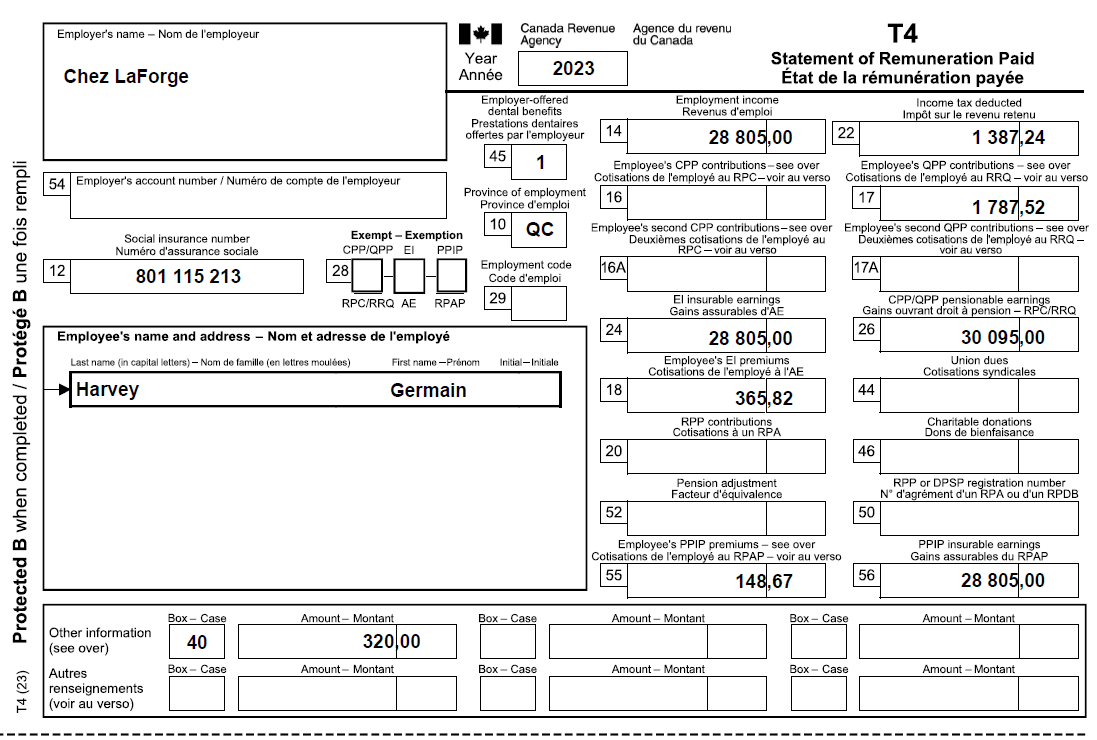
\includegraphics[width=.96\textwidth]{exercice/2.6/Q1/a-T4.png}
		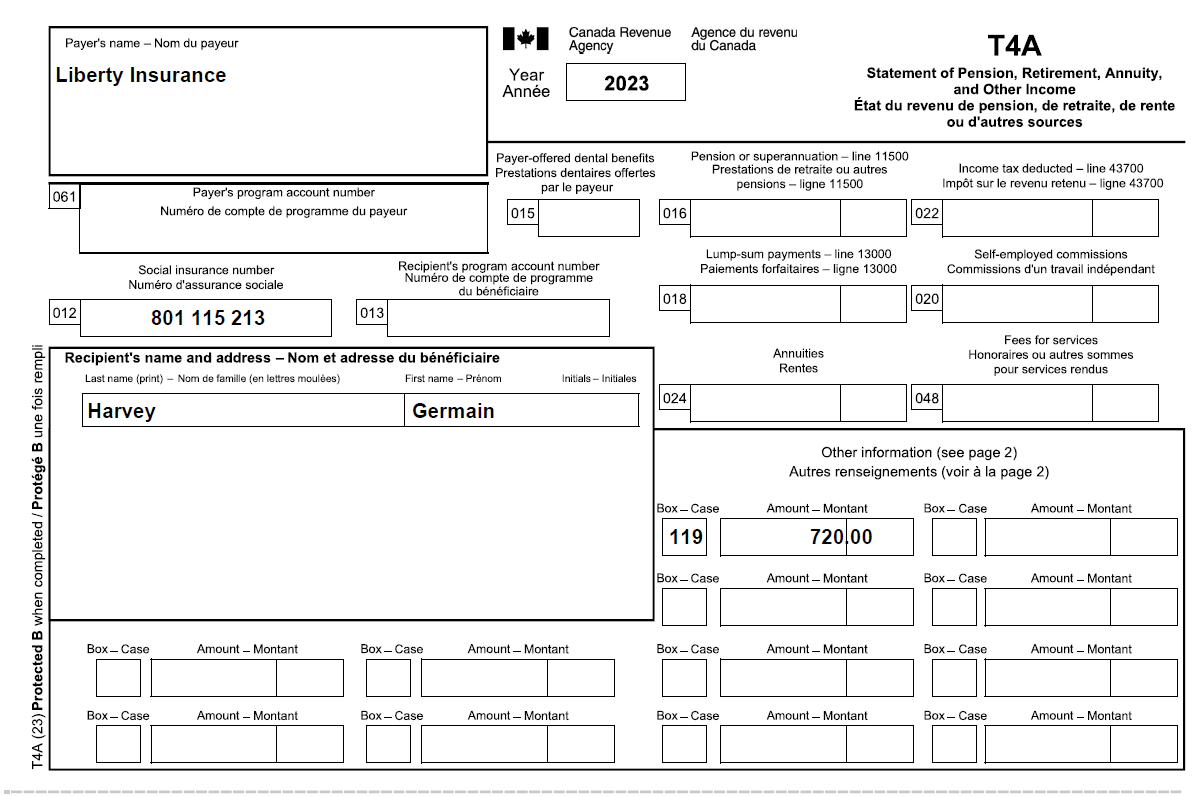
\includegraphics[width=.96\textwidth]{exercice/2.6/Q1/a-T4A.png}
	\end{center}
	
	\noindent
	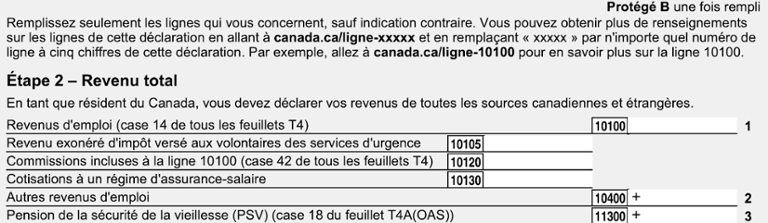
\includegraphics[width=\textwidth]{exercice/2.6/Q1/a-T1.png}
\end{sousQuestion}
\noindent
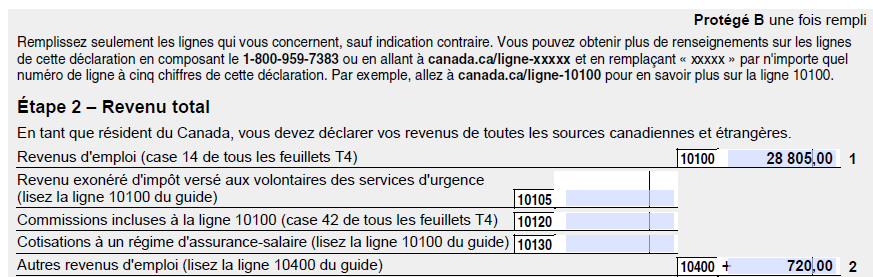
\includegraphics[width=\textwidth]{exercice/2.6/Q1/a-reponse.png}

\begin{sousQuestion}
	Germain Harvey a également reçu les feuillets Relevés 1 et 22. Effectuez la correction de son revenu d'emploi à l'aide de la grille de calcul 105. Inscrivez les montants aux cases et lignes de 94 à 105 qui doivent être remplies sur la TP-1
	\begin{center}
		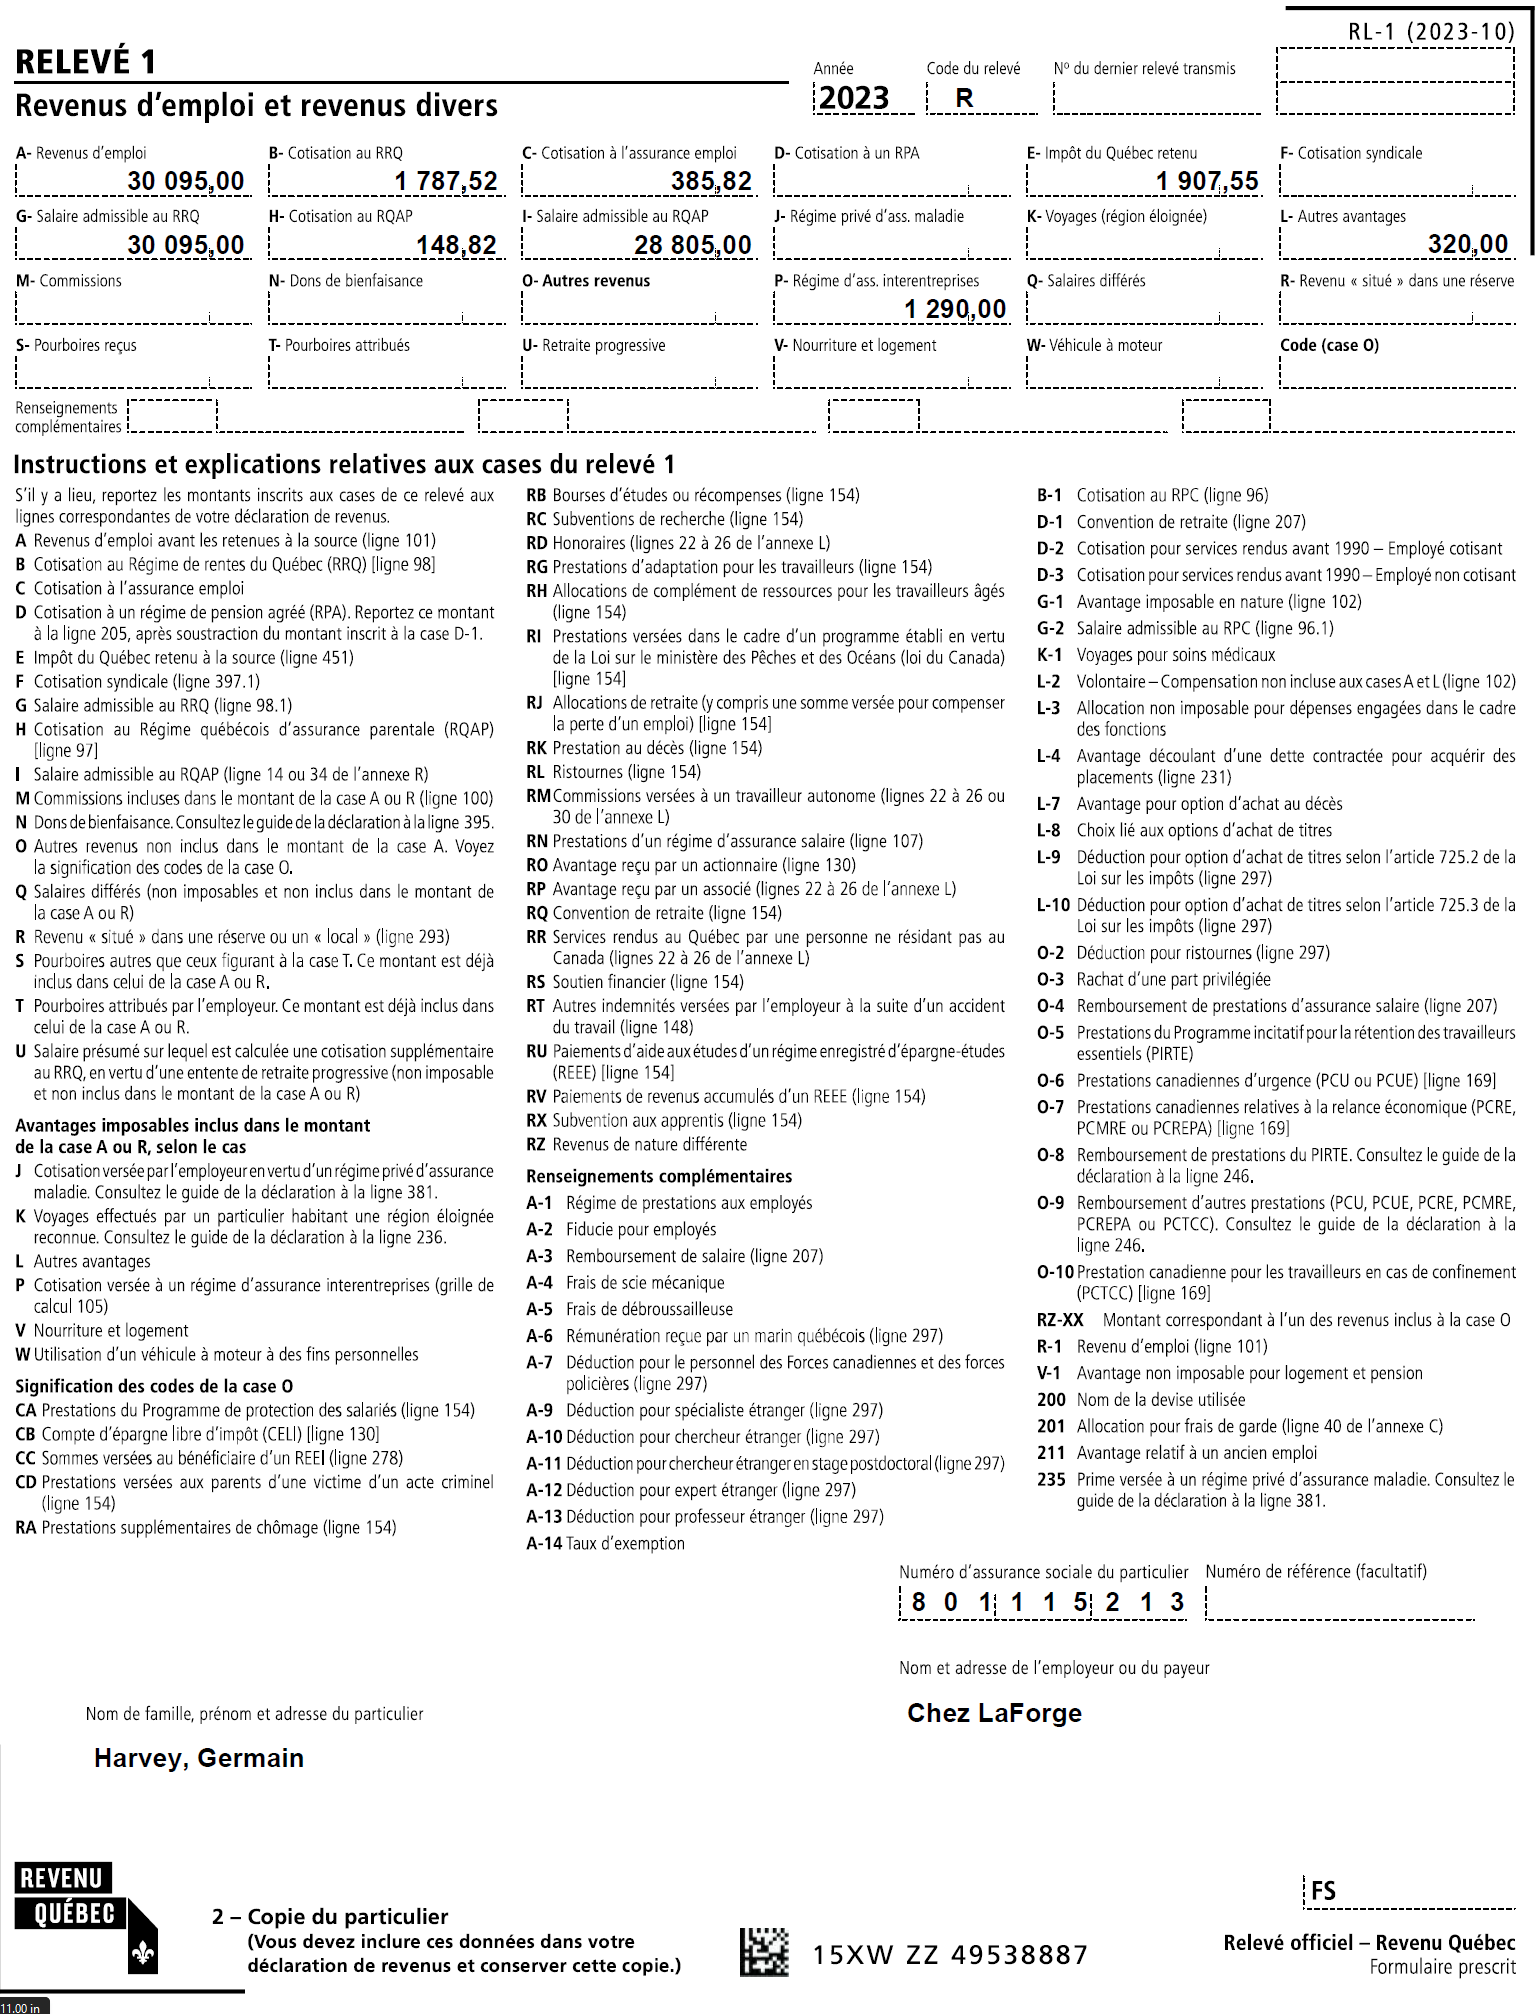
\includegraphics[width=.96\textwidth]{exercice/2.6/Q1/b-RL1.png}
		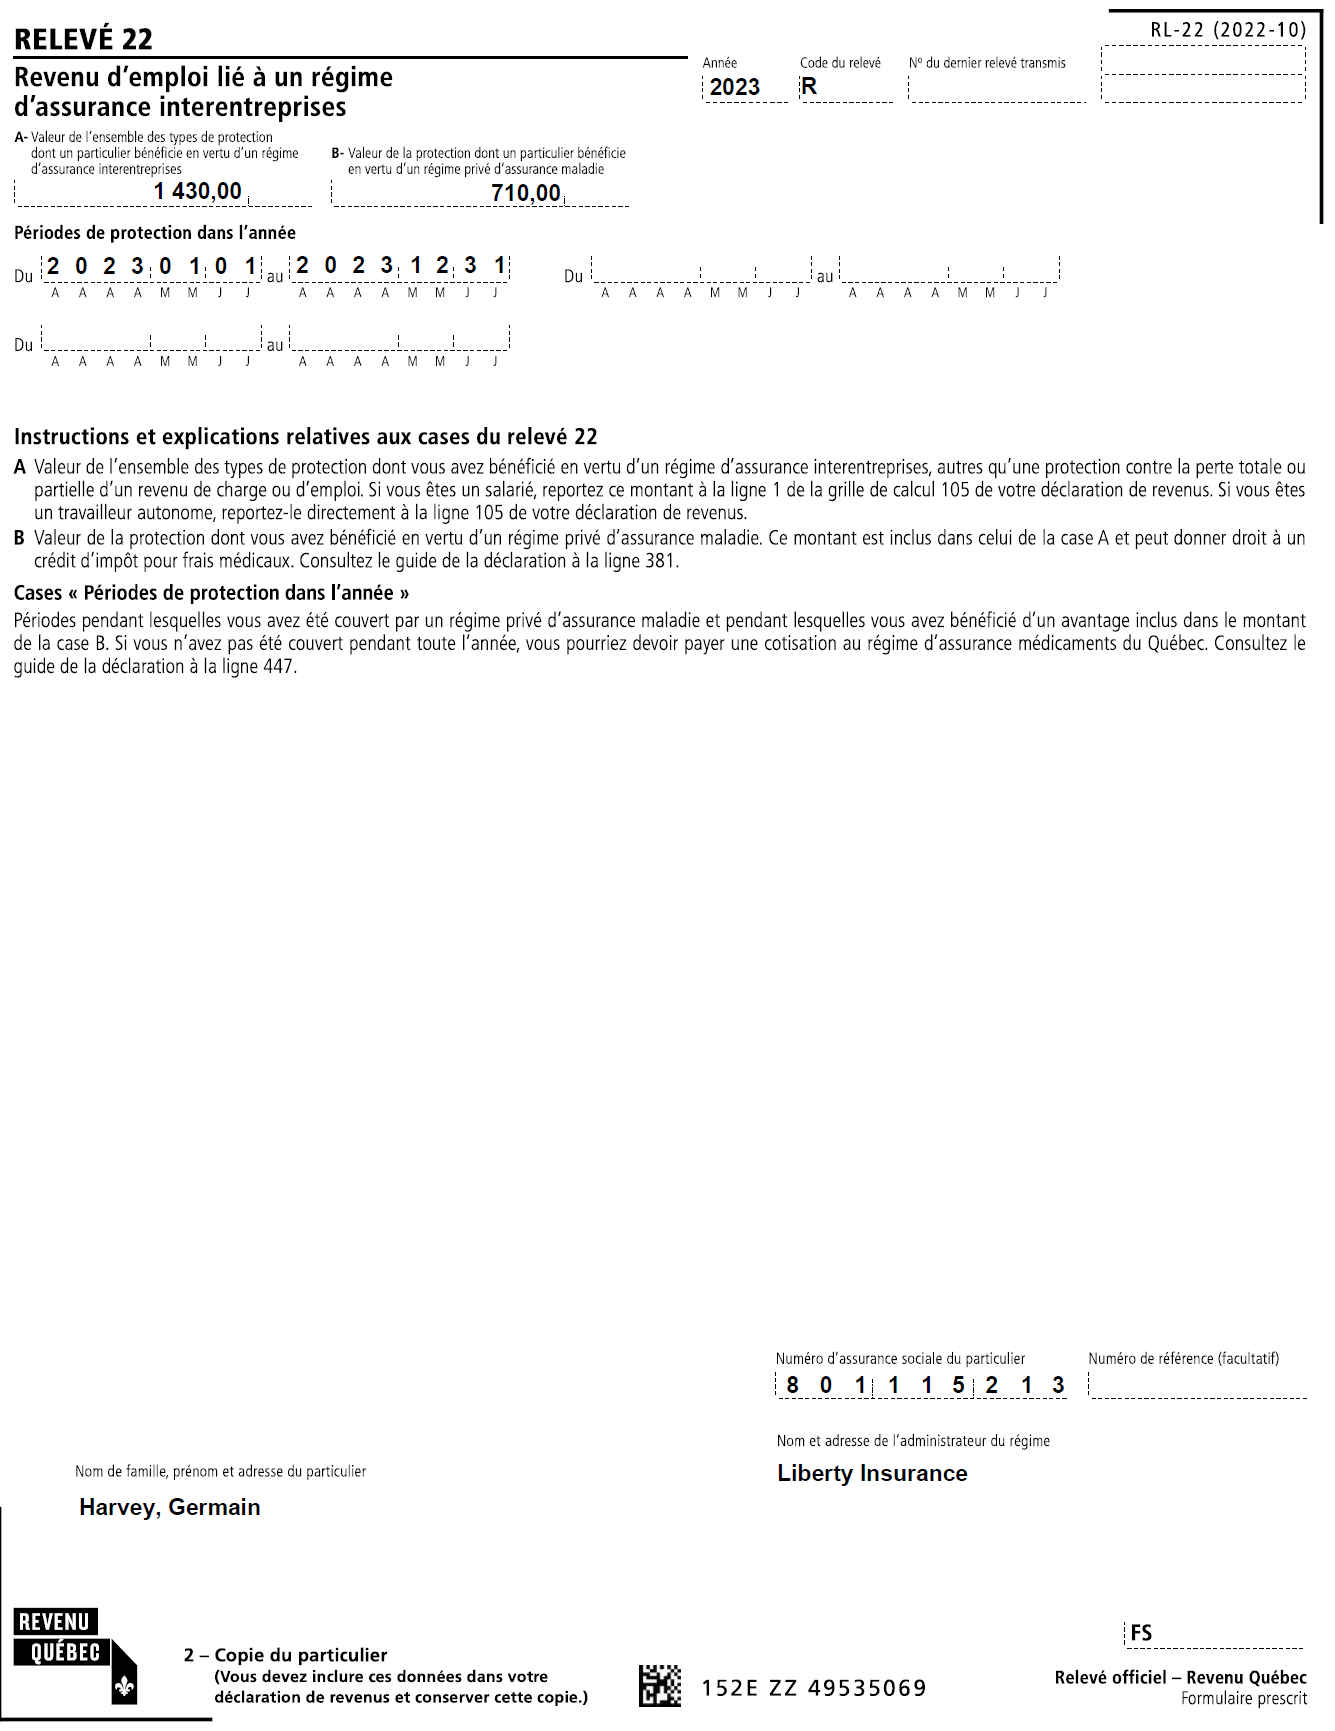
\includegraphics[width=.96\textwidth]{exercice/2.6/Q1/b-RL22.png}
	\end{center}
	
	\noindent
	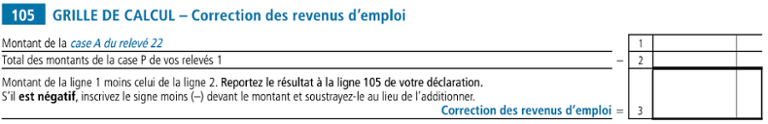
\includegraphics[width=\textwidth]{exercice/2.6/Q1/b-105.png}
	
	\noindent
	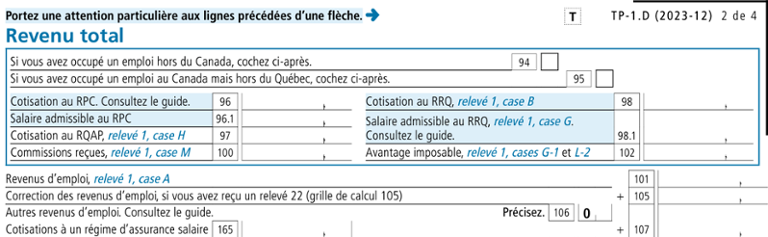
\includegraphics[width=\textwidth]{exercice/2.6/Q1/b-TP1.png}
\end{sousQuestion}
\noindent
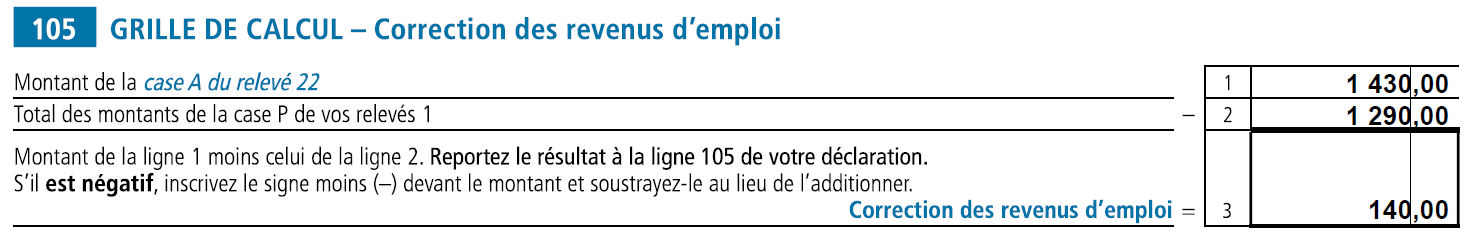
\includegraphics[width=\textwidth]{exercice/2.6/Q1/b-105-reponse.png}

\noindent
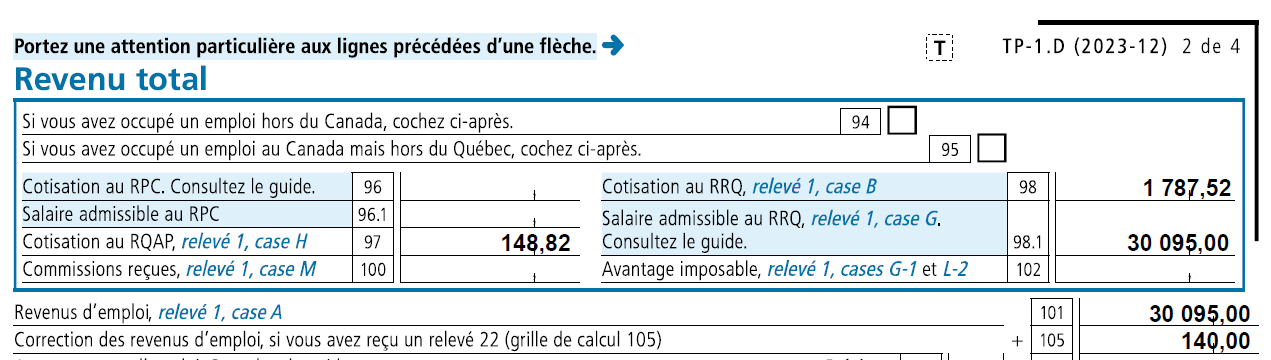
\includegraphics[width=\textwidth]{exercice/2.6/Q1/b-TP1-reponse.png}

\begin{question}
	Charlotte Landry habite au 1275 rue Giguère, Québec, QC, G1P 1Z6 toute l’année. Son NAS est le 805 101 813 et sa date de naissance est le 5 février 1981. Elle est mariée à Gerald Landry, dont le NAS est le 805 101 821 et la date de naissance est le 15 juillet 1982, et son revenu total en 2023 était de \numprint{22480} \$. Charlotte et Gerald ne sont pas des travailleurs autonomes. Les Landrys n’ont pas d’enfants.

L’adresse courriel de Charlotte est clandry@videotron.ca et elle consent à recevoir de la correspondance en français par voie électronique uniquement.

Complétez les pages 1 des feuillets T1 et TP-1 de Charlotte Landry.
	
	\begin{center}
		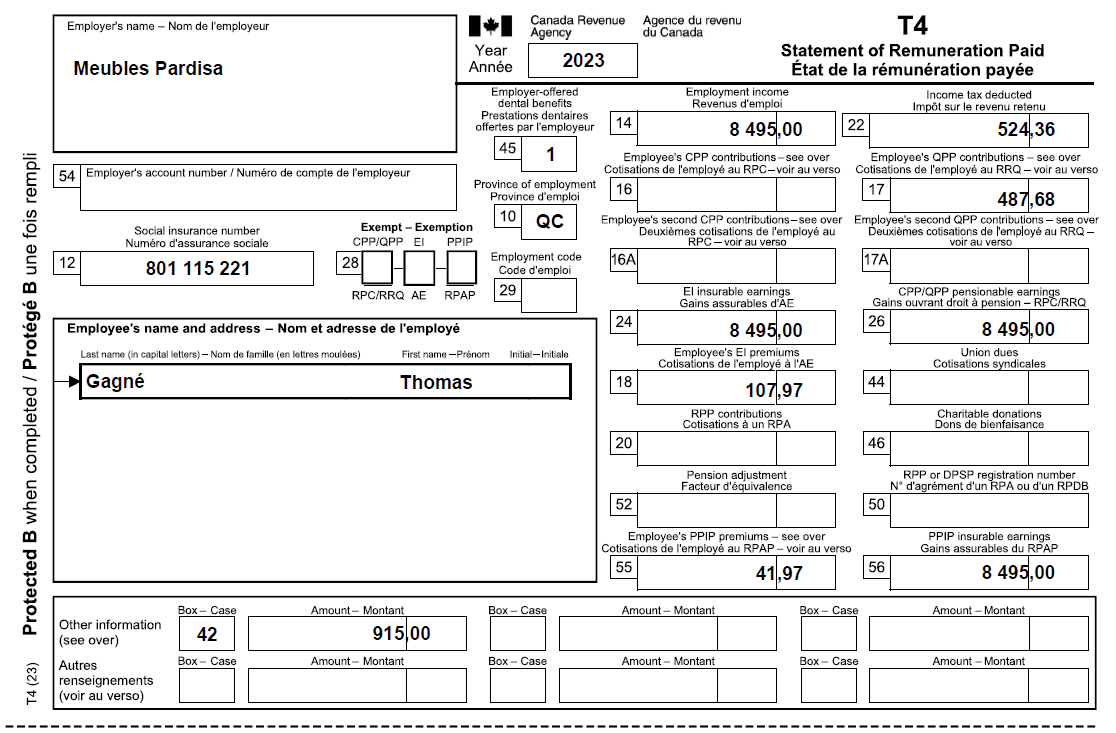
\includegraphics[width=.97\textwidth]{exercice/2.6/Q2/T4-1.png}
		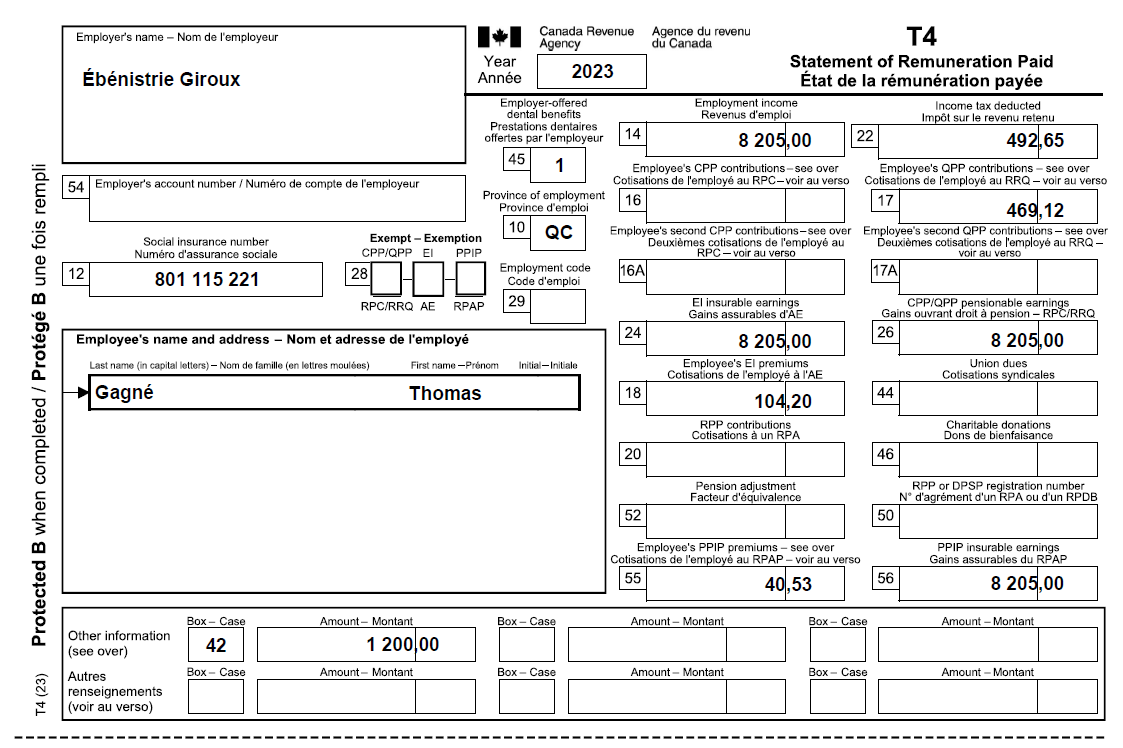
\includegraphics[width=.97\textwidth]{exercice/2.6/Q2/T4-2.png}
	\end{center}
\end{question}
\[ \text{Ligne 10100} = 8495 + 8205 = 16700\]
\[ \text{Ligne 10120} = 915 + 1200 = 2115\]

\begin{question}
	Certains revenus d'emploi sont reportés aux lignes 10100 de la T1 et 101 de la TP-1, tandis que d'autres sont reportés aux lignes 10400 de la T1 et 107 de la TP-1. 
	
	Si on vous a versé un revenu d'emploi, comment pouvez-vous savoir à quelle ligne vous devez le déclarer?
\end{question}
Si le revenu d'emploi est indiqué aux cases 14 du T4 et A du relevé 1, il doit être reporté aux lignes 10100 de la T1 et 101 la TP-1.

Règle générale, tous les autres revenus liés à l'emploi, qui ne figurent pas sur des feuillets, sont reportés à la ligne 10400 de la T1 et à la ligne 107, code \og 05\fg{} à la case 106, de la TP-1.

Certaines exceptions existent.
D'autres sources de revenus peuvent s'inscrire aux lignes 13000 de la T1 et 154 de la TP-1.

Si vous n'avez pas en main les endos des feuillets d'impôts, consulter alors les guides de déclarations de revenus pour en savoir plus long.

\begin{question}
	Alain a gagné un revenu d'emploi de \numprint{10300}~\$, indiqué aux cases 14 de son T4 et A de son relevé 1. Durant l'année d'imposition, il a également reçu \numprint{2350}~\$ de pourboires qui ne sont pas indiqués nulle part sur ses feuillets.
\end{question}
\setcounter{sousQuestion}{0}
\begin{sousQuestion}
	D'après Alain, il doit déclarer seulement les revenus indiqués sur des feuillets. Puisqu'il n'a aucun feuillet indiquant le montant de ses pourboires, il est convaincu qu'il n'est pas tenu de les déclarer. 
	
	Est-ce qu'il a raison? Expliquez votre réponse.
\end{sousQuestion}
Non. Alain a tort.

La loi exige que le contribuable déclare ses revenus de toutes les sources, peu importe qu'ils soient inscrits sur des feuillets ou pas, sauf pour les montants mentionnés dans le chapitre 1 qui sont spécifiquement exonérés d'impôt et exclus du revenu.

Les pourboires qui ne figurent pas sur des feuillets doivent être déclarés aux lignes 10400 de la T1 et 107, code \og 01\fg{} à la case 106, de la TP-1.

\begin{sousQuestion}
	Auxquelles lignes de la T1 et de la TP-1, les informations ci-dessus doivent-elles être déclarées. Incluez le code correspondant sur la TP-1, s'il y a lieu.
\end{sousQuestion}

\numprint{10300}~\$: T1.10100 et TP-1.101

\numprint{2350}~\$: T1.10400 et TP-1.107 + TP-1.106 = 01

\begin{question}
	Auxquelles lignes des déclarations T1 et TP-1 doivent être reportés les revenus suivants? 
	Incluez le code correspondant sur la TP-1, s'il y a lieu.
	\begin{itemize}
		\item Pourboires reçus (pas sur T4 ni RL-1)
		\item Revenus de gardiennage (2 jours par mois)
		\item Travail temporaire (850 \$)
	\end{itemize}
\end{question}
\begin{itemize}
	\item Pourboires: T1.10400, TP-1.107, TP-1.106 = 01
	\item Gardiennage d'enfants: T1.10400, TP-1.107, TP-1.106 = 05
	\item Travail temporaire: T1.10400, TP-1.107, TP-1.106 = 05
\end{itemize}



\section{Régimes d'assurance de sécurité du revenu en cas de maladie ou de perte d'emploi}
\begin{intro}
	Il existe différents types de régimes de maladie, d'accident, d'invalidité et de maternité qui fournissent des prestations aux employés en raison de la perte de revenus lorsqu'ils sont malades, blessés, invalides, enceintes ou licenciés.
	
	Il s'agit de régimes privés, qui ne relèvent ni du Régime des rentes du Québec ni du régime fédéral d'assurance-emploi. 
	
	Les revenus ou les prestations de ces régimes peuvent être entièrement imposables, partiellement imposables ou exonérés d'impôt.
\end{intro}


\subsection{Prestation d'assurance salaire ou prestation d'assurance collective contre la maladie ou les accidents}
\begin{enumerate}
	\item L'employeur a payé toutes les cotisations
	\begin{enumerate}
		\item Si l'employeur finance le régime, exerce un contrôle et détermine les critères d'admissibilité, alors les prestations seront assujetties à des retenues à la source (cotisations RRQ, RQAP, assurance emploi et impôts).
		
		Il est déclaré à la ligne 10100 de la T1 et à la ligne 101 de la TP-1.
		\item Si l'employeur finance le régime, mais que celui-ci est contrôlé par un administrateur externe, l'administrateur émet alors un feuillet T4A (case 107) et un Relevé 1 (case O, code RN  dans la case Code (case O) ). Ce revenu n'est pas assujetti aux déductions pour le RRQ, l'AE ou le RQAP.
		
		Le montant total reçu est imposable et doit être déclaré aux lignes 10400 de la T1 et 107, code 02 à la case 106 de la TP-1.
	\end{enumerate}
	\item L'employé a payé toutes les cotisations, aucun feuillet ne sera émis, car aucun des avantages reçus n'est imposable. Le montant reçu n'a pas à être inscrit sur les déclarations de l'employé.
	\item Si l'employeur et l'employé ont tous deux versé des primes au régime, les feuillets de renseignements émis sont similaires à ceux décrits dans l'option 1, en fonction de la personne qui exerce le contrôle sur le plan.
	\begin{enumerate}
		\item Si l'employeur exerce un contrôle sur le régime, le revenu est inclus dans la case 14 du T4 et dans la case A du Relevé-1
		
		Toutefois, l'employé peut soustraire de la ligne 10100 de la T1 et de la ligne 101 de la TP-1 tout ou partie des primes inutilisées qu'il a versées au régime. Parallèlement, ce montant de réduction doit être inscrit à la ligne 10130 de la déclaration T1.
		\item Si le régime est contrôlé par un administrateur externe, celui-ci émet un feuillet T4A et un Relevé 1 (case O, code RN  dans la case Code (case O)).
		
		Dans ce cas, l'employé peut soustraire la totalité ou une partie de ses primes inutilisées du montant inscrit à la case 107 du T4A et inscrire le montant réduit à la ligne 10400 de la T1. De même, le montant de la case O du Relevé 1 est réduit en conséquence et reporté à la ligne 107, code \og 02\fg{} de la case 106 du TP-1. Notez que dans cette situation, il n'y a pas de ligne équivalente à la ligne 10130 cependant, la ligne 165 est utilisée sur le TP-1 pour inscrire les primes utilisées en tant que réduction.
	\end{enumerate}
\end{enumerate}

\subsubsection{Régime de prestations supplémentaires de chômage}
Les avantages imposables de ce régime enregistré figurent sur un T4A à la case 152. Au Québec, ils sont inscrits à la case O du Relevé1 et le code RA se trouve à la case Code (case O) du Relevé1. Le montant doit être déclaré aux lignes 10400 de la T1 et 154, le code 03  à la case 153 de la TP-1.

Si un régime de prestations supplémentaires de chômage n'est pas inscrit au Programme de prestations supplémentaires de chômage (PSC), les montants versés sont inclus dans les cases 14 du T4 et A du Relevé 1. Ils doivent ensuite être déclarés à la ligne 10100 de la T1 et à la ligne 101 de la TP-1 des déclarations de revenus en tant que revenus d'emploi.

\subsubsection{Régime de participation des employés aux bénéfices}
Dans la déclaration fédérale, ces montants reçus sont indiqués à la case 35 Autres revenus d'emploi du feuillet T4PS. Ils doivent être déclarés à la ligne 10400 de la déclaration T1.

Au Québec, on regarde si le revenu est assujetti ou non à une cotisation au RRQ. Ceci est déterminé par les cases Renseignements complémentaires du Relevé 25 comme suit:

Inscrivez à la ligne 101 de la déclaration TP-1, si le montant figure également à la case D-1 du Relevé 25. Ce montant fait l'objet d'une cotisation au RRQ.
Inscrivez à la ligne 107, code 03 à la case 106 de la TP-1 si le montant figure également à la case D-2 du Relevé 25. Ce montant n'est pas assujetti à une cotisation au RRQ.

\begin{note}
	Ces régimes peuvent inclure des dividendes, des gains en capital, et des revenus de source étrangère.
\end{note}

\subsubsection{Paiements provenant du programme de protection des salariés}
Dans la déclaration fédérale, le montant figure à la case 132 du T4A. Au Québec, il figure à la case O du Relevé1, avec le code CA dans la case  Code (case O). Il doit être déclaré aux lignes 10400 de la T1 et 154, code 12 à la case 153 de la TP-1.



\section{Subventions et redevances}
\begin{intro}
	Les subventions permettant de mener des recherches, les subventions en reconnaissance d'une réalisation et certaines redevances sont considérées comme d'autres revenus d'emploi.
\end{intro}


\subsection{Subventions de recherche}
Lorsque l'employeur verse la subvention, toute portion qui représente un revenu est déclarée sur un T4 et un Relevé 1.

Sinon, la subvention est déclarée à la case 104 du T4A et à la case O du Relevé 1. Comme la case O est utilisée pour de nombreux types de revenus, une information supplémentaire est fournie dans la case Code (case O) pour indiquer le type de revenu reçu. Pour les subventions de recherche, le code est RC. 

Le contribuable qui a reçu une subvention de recherche peut déduire les dépenses payées ou encourues pour la réalisation de son projet:
\begin{itemize}
	\item Frais de déplacement (y compris les repas et l'hébergement) pour les voyages de recherche
	\item Frais de laboratoire
	\item Achat d'équipement/de fournitures
	\item Salaire versé à un assistant
\end{itemize}

Les dépenses suivantes ne sont pas déductibles:
\begin{itemize}
	\item Les dépenses personnelles et de subsistance, autres que les frais de déménagement
	\item Les dépenses pour lesquelles le contribuable a reçu un remboursement, à moins que le remboursement ne soit inclus dans la subvention
	\item Les coûts déductibles déjà pris en compte dans le calcul du revenu
\end{itemize}

\rqg{30 \S j}


\subsection{Subvention incitative aux apprentis (SIA)}
Déclaré à la case 130 du T4A. Inscrit à la ligne 13000 de la T1. Déclaré dans la case O du Relevé 1 en utilisant le code RX. Inscrit à la ligne 154 de la TP-1 en utilisant le code 03.


\subsection{Subvention à l'achèvement de la formation d'apprenti (SAFA)}
Déclaré à la case 130 du T4A. Inscrit à la ligne 13000 de la T1. Déclaré dans la case O du Relevé 1 en utilisant le code RX. Inscrit à la ligne 154 de la TP-1 en utilisant le code 03.

\href{https://www.red-seal.ca/fra/w.2lc.4m.2.shtml}{Programme Sceau rouge}


\subsection{Redevances provenant d'une œuvre ou d'une invention}
Ces redevances sont inscrites à la case 17 du T5, État des revenus de placements, et à la case H du Relevé 3, Revenus de placements.

Au niveau fédéral, il existe différents traitements: 
\begin{itemize}
	\item Si elles sont reçues pour un travail ou une invention du contribuable, les redevances doivent être déclarées à la ligne 10400 de la T1, c'est-à-dire en tant qu'autres revenus d'emploi.
	\item Sinon, elles doivent être déclarées à la ligne 12100, qui est classée comme Intérêts et autres revenus d'investissement.
\end{itemize}

Au Québec, les deux doivent être déclarés à la ligne 130 de la TP-1 en tant qu'intérêts et autres revenus d'investissement.



\section{Revenu total}
En supposant que le contribuable n'a aucun autre revenu, on inscrit le total des lignes 10100, 10400 et 13000 à la ligne 15000 de la T1.

Au Québec, c'est à la ligne 199 qu'on doit inscrire le total des lignes 101, 105, 107 et 154.



\section{Exercice 2-7}
\setcounter{question}{0}
\begin{question}
	Roger a été en arrêt de travail pour cause de maladie pendant une période de quatre mois.
	
	Son T4A et son Relevé 1 indiquent qu'il a reçu \numprint{1600}~\$ en prestations d'un régime d'assurance-salaire. Il a versé des cotisations annuelles de \numprint{200}~\$ au régime au cours des cinq dernières années. Son employeur a également cotisé au régime au cours de chacune de ces années, mais il n'exerce pas de contrôle. 
	
	Dans l'espace ci-dessous, calculez le montant et indiquez sur quelles lignes ce montant doit être inscrit sur les déclarations T1 et TP1 de Roger, en supposant qu'il s'agit de la première année où il a reçu des prestations du régime.
\end{question}
Le calcul doit être effectué comme suit:

\begin{itemize}
	\item Montant reçu (T4A et Relevé 1): \numprint{1600}~\$
	\item Moins: total des cotisations de l'employé versées au régime (5 x 200~\$): \numprint{1000}~\$ 
	\item Montant à déclarer à la ligne 10400 de la T1 et à la ligne 107 de la TP-1, en utilisant le code 02 à la case 106: 600~\$
\end{itemize}

Les primes soustraites de la prestation doivent être inscrites à la ligne 165 du formulaire TP-1.

\begin{question}
	Gilles Fortin est professeur à l'Université de Montréal. Au cours de l'année d'imposition, il a reçu une subvention de recherche de \numprint{38000}~\$ de l'université, pour laquelle il a reçu un T4A et un
	Relevé 1.
	
	Il a payé un assistant \numprint{10000}~\$ pour effectuer une partie de la recherche.
	Si le Dr Fortin n'a pas d'autres dépenses applicables, quel montant de la subvention de recherche doit-il déclarer dans sa déclaration, et sur quelles lignes?
\end{question}
Il doit déclarer le montant net de la subvention, c'est-à-dire la subvention moins les dépenses admissibles. Il doit donc inscrire \numprint{28000}~\$ (\numprint{38000}~\$ $-$ \numprint{10000}~\$) à la ligne 10400 de la T1 et à la ligne 154 de la TP-1, avec le code 03 à la case 153.



\section{Sommaire du chapitre 2}
\begin{itemize}
	\item La section d'identification de la Déclaration de revenus et de prestations et de la Déclaration de revenus servent à identifier le contribuable et à fournir des informations personnelles qui ont une incidence sur le calcul de l'impôt.
	\item Les questions d'Élections Canada permettent à l'ARC de fournir des informations personnelles sélectionnées pour mettre à jour le Registre national des électeurs.
	\item La question relative aux biens étrangers vise à encourager le respect de l'obligation de déclarer les revenus provenant de biens étrangers déterminés.
	\item L'usage de certaines cases des principaux feuillets d'impôts, soit le T4 et le Relevé 1.
	\item Les autres revenus tels que redevances, subventions de recherche, prestations supplémentaires de chômage, etc.
	\item La demande du Crédit d'impôt pour solidarité au Québec.
	\item La différence entre un revenu d'emploi d'un salarié et celui d'un travailleur autonome.
	\item Un aperçu des différents feuillets d'impôt tels le T4A, Relevé 22.
	\item La présence de grilles de calcul pour effectuer des opérations mathématiques dont le résultat s'inscrit directement sur la déclaration, notamment la grille 105 sur la correction d'emploi.
	\item Les revenus sans feuillets de renseignements. 
	\item Les prestations d'assurance-emploi, dont les situations sont diverses.
\end{itemize}% Revenus et dépenses d'emploi
\chapter{Déductions et crédits d'emploi}
\section{Introduction et objectifs}
\subsection{Introduction}
Déductions et crédits qui s'appliquent au revenu d'emploi. On retrouve les déductions dans deux parties des T1 et TP-1: le calcul du revenu net et le calcul du  revenu imposable. De plus, nous étudierons certains crédits d'impôt non remboursables reliés à l'emploi qui peuvent être réclamés à l'étape~5 de la T1, ainsi qu'à la page 3 de la TP-1.


\subsection{Objectifs}
\begin{itemize}
	\item Expliquer ce qu'on entend par déduction pour travailleur et comment la réclamer;
	\item Réclamer la déduction pour un régime de pension agréé;
	\item Réclamer la déduction fédérale et le crédit d'impôt non remboursable du Québec relativement aux cotisations syndicales, professionnelles et autres cotisations semblables;
	\item Réclamer les dépenses d'emploi liées au travail à domicile en raison de la COVID-19;
	\item Expliquer comment le contribuable qui déménage pour occuper un emploi dans un nouveau lieu de travail peut réclamer des frais de déménagement;
	\item Réclamer la déduction pour remboursement de salaires ou de prestations d'assurance salaire;
	\item Réclamer la déduction pour le personnel des Forces canadiennes et des forces policières;
	\item Réclamer la déduction pour options d'achat de titres pour les employés;
	\item Réclamer la déduction pour ristourne reçue d'une coopérative;
	\item Réclamer la déduction pour revenu d'emploi gagné sur un navire;
	\item Calculer la cotisation que doit verser un employé au Régime de rentes du Québec (RRQ) et déterminer les cotisations versées en trop;
	\item Réclamer une déduction pour la cotisation bonifiée au RRQ sur un revenu d'emploi; 
	\item Calculer la cotisation que doit payer un employé au Régime québécois d'assurance parentale et déterminer les cotisations versées en trop;
	\item Calculer la cotisation que doit verser un employé à l'assurance-emploi et déterminer les cotisations versées en trop;
	\item Réclamer le montant canadien pour emploi;
	\item Réclamer le crédit d'impôt non remboursable pour pompiers volontaires ou volontaires participant à des activités de recherche et de sauvetage;
	\item Appliquer les règles régissant qui doit déclarer un revenu rétroactif de la Prestation universelle pour la garde d'enfants (PUGE) fédérale; 
	\item Réclamer le crédit d'impôt non remboursable pour les nouveaux diplômés travaillant dans une région ressource éloignée.
\end{itemize}


\subsection{Sujets du chapitre 3}
\begin{itemize}
	\item Déductions
	\item Déductions du revenu d'emploi
	\item Revenu net et imposable
	\item RRQ, RQAP et AE
	\item Crédits non remboursables pour revenu d'emploi
\end{itemize}



\section{Distinction entre déductions et crédits d'impôt}
\begin{intro}
	La première partie de ce chapitre concerne les déductions les plus communes qui sont reliées à l'emploi. L'application de ces déductions conduit au calcul du revenu net.
	
	La deuxième partie de ce chapitre concerne les déductions plus spécifiques qui sont aussi reliées à l'emploi. Celles-ci ne concernent que quelques contribuables. L'application de ces déductions fiscales spécifiques, conduit au calcul du revenu imposable.
	
	Enfin, la troisième partie de ce chapitre concerne les crédits d'impôt non remboursables qui sont reliés à l'emploi. Pour cette partie, nous verrons ceux pour le fédéral en particulier.
	
	Il est important de comprendre les différences entre les déductions et les deux types de crédits (remboursables et non remboursables) et comment ils sont utilisés dans le calcul de l'impôt sur le revenu.
\end{intro}
\begin{note}
	Les trousses d'impôt comprennent des guides qui fournissent des explications pour remplir chaque déclaration de revenus. Dans la transition vers le monde numérique, le guide fédéral a constaté une réduction des explications ligne par ligne. Si vous ne trouvez pas d'explication dans le guide, utilisez le champ de recherche sur le site Web de l'ARC et entrez le numéro de ligne.
	
	Cliquez sur le bouton ci-dessous pour afficher une liste complète de chaque ligne dans les étapes 3 à 6.
	
	\cat\href{https://www.canada.ca/fr/agence-revenu/services/impot/particuliers/sujets/tout-votre-declaration-revenus/declaration-revenus/remplir-declaration-revenus/deductions-credits-depenses/toutes-deductions-tous-credits-toutes-depenses.html}{Toutes les déductions, tous les crédits et toutes les dépenses}
\end{note}


\subsection{Déduction}
Une déduction réduit le revenu assujetti à l'impôt et, par conséquent, réduit en fin de compte l'impôt qu'une personne doit payer.

Il existe deux séries de déductions. Le premier ensemble réduit le revenu total dans le calcul du revenu net. Il se trouve à l'étape~3 - Revenu net de la T1 et à la section \og Revenu net \fg{} de la TP-1. 

Le deuxième ensemble de déductions réduit le revenu net dans le calcul du revenu imposable. Il se trouve à l'étape~4 - Revenu imposable de la T1 et à la partie \og Revenu imposable \fg{} de la TP-1.


\subsection{Crédits d'impôt non remboursables}
En ce qui concerne les crédits d'impôt non remboursables, ils servent à réduire l'impôt à payer plutôt que le revenu. 

Les crédits d'impôt ont la même valeur pour tous puisqu'ils sont accordés à un taux fixe pour tous les contribuables, peu importe leur revenu et leur taux marginal d'imposition. 

Les crédits d'impôt non remboursables sont déterminés pour la déclaration fédérale dans la partie des crédits d'impôt non remboursables à la section 5 de la T1, puis convertis au taux de 15~\%. D'autres crédits d'impôt non remboursables ont des taux différents, qui seront calculés plus tard, notamment dans la Partie C - Impôt fédéral net de l'étape~5 de la T1.

Au Québec, les crédits non remboursables peuvent être réclamés dans deux parties, les crédits d'impôt non remboursables et les revenus et cotisations à la page 3 du TP-1. Pour de nombreux crédits, le taux est de 14~\%, cependant il existe une fourchette de taux plus large que le fédéral variant entre 8~\% et
30~\% selon les crédits.

Si la valeur totale des crédits non remboursables est égale ou supérieure à l'impôt à payer, le contribuable ne tire aucun avantage du surplus. C'est pourquoi ils sont appelés non remboursables.

Au Québec, cependant, nous verrons dans un chapitre ultérieur comment un conjoint ayant un excédent de crédits non remboursables peut les transférer à sa conjointe si elle est en mesure d'utiliser l'excédent. 


\subsection{Crédits d'impôt remboursables}
Les crédits remboursables sont également utilisés pour réduire l'impôt à payer plutôt que le revenu. 

Toutefois, si un surplus est créé lorsque ces crédits sont appliqués à l'impôt à payer, ce surplus est retourné au contribuable sous forme de remboursement. 

Ceux-ci sont réclamés à l'étape~6 - \og Remboursement ou solde dû \fg{} de la T1 et \og Remboursement ou solde à payer \fg{} de la TP-1. 

Il existe deux types de crédits remboursables: 
\begin{itemize}
	\item Le premier type est des crédits pour des montants qu'un contribuable a déjà payés ou payés en trop. Le plus souvent, ces montants étaient déduits à la source; 
	\item Le deuxième type englobe les crédits d'impôt accordés par les gouvernements pour des programmes de redistribution des revenus ou de promotion de certains objectifs et politiques sociales.
\end{itemize}



\section{Calcul du revenu net}
\begin{intro}
	Le revenu net est déterminé en appliquant les déductions admissibles au montant du Revenu total. 
	
	Dans cette partie, vous découvrirez les déductions les plus courantes liées à l'emploi.
\end{intro}
Après avoir déterminé son revenu total, un contribuable doit identifier toutes les déductions auxquelles il est admissible.

Dans cette 1ère partie de chapitre, nous étudions les déductions qui sont reliées à un revenu d'emploi. Elles comprennent, entre autres:
\begin{itemize}
	\item La déduction pour travailleur, au Québec seulement;
	\item La déduction pour un régime de pension agréé;
	\item Les cotisations annuelles syndicales et professionnelles (sujet spécial);
	\item Déduction pour la cotisation bonifiée au RRQ sur un revenu d'emploi; 
	\item Les frais de déménagement.
\end{itemize}

Au fédéral, on déduit le remboursement des prestations de programmes sociaux à la ligne~23500.

Le revenu net est utilisé pour déterminer l'admissibilité du contribuable à certains crédits d'impôt et prestations sociales.

\begin{note}
	Sur les des déclarations fédérale et du Québec, le contribuable additionne toutes les déductions auxquelles il a droit, puis soustrait simplement le résultat du revenu total pour obtenir le revenu net.
	
	Étant donné que les déductions sur la déclaration fédérale et celle du Québec ne sont pas toujours les mêmes, il est tout à fait normal que les montants du revenu net soient différents.
\end{note}



\section{Déduction pour travailleurs}
\begin{intro}
	Le gouvernement du Québec offre à tous les contribuables ayant un revenu d'emploi une compensation financière afin d'assumer les petites dépenses quotidiennes reliées à l'emploi.
\end{intro}

Au Québec, sur la TP-1, le contribuable ayant un revenu d'emploi peut bénéficier d'une déduction pour travailleur correspondant à 6~\% du revenu de travail admissible, jusqu'à concurrence de \numprint{1315}~\$ pour l'année d'imposition 2023. 

Cette déduction se calcule sur la grille de calcul 201. Elle est réclamée à la ligne~201, réduisant ainsi le revenu net.

Les revenus de travail donnant droit à la déduction pour travailleurs comprennent:
\begin{itemize}
	\item Revenus d'emploi des lignes~101, 107 et si positif, ligne~105;
	\item Le montant net des subventions de recherche;
	\item Prestations du Programme de protection des salariés (sera discuté au chapitre 7);
	\item Montants reçus dans le cadre d'un projet d'incitation au travail.
\end{itemize}
\begin{note}
	Le revenu d'emploi composé uniquement d'avantages imposables obtenus en raison d'un emploi antérieur, ne constitue pas un revenu admissible aux fins de cette déduction. Le montant inscrit à la case~211 du relevé~1 doit être soustrait du montant inscrit à la ligne~101.
\end{note}
Sur la déclaration T1, l'équivalent de cette déduction est le Montant canadien pour emploi, qui est un crédit non remboursable.
\begin{note}
	Lorsque les revenus d'emploi sont supérieurs à \numprint{21916,67}~\$, la déduction maximum est de \numprint{1315}~\$.
\end{note}



\section{Régime de pension agréé (RPA)}
\begin{intro}
	Un \acrfull{rpa} est un régime de pension enregistré auprès de l'ARC conformément à la Loi de l'impôt sur le revenu. Le régime est mis en place par un employeur pour fournir un revenu de pension à ses employés au moment de leur retraite
\end{intro}
Les cotisations qui peuvent être versées à un RPA comprennent les cotisations pour services courants et celles pour services passés:
\begin{itemize}
	\item Service courant en 2023
	\item Service antérieur de 1990 à 2022
	\item Service antérieur pour 1989 et les années précédentes.
	\item 
\end{itemize}


\subsection{Déduction pour cotisations pour services courants}
Le montant retenu par l'employeur est indiqué aux cases~20 du feuillet T4 et D du relevé~1. Il peut également figurer sur un reçu émis par le syndicat du travailleur.

Une déduction peut être réclamée aux lignes~20700 de la déclaration T1 et 205 de la TP1.

Si un montant paraît à la case~52 du feuillet T4 et qu'aucun montant n'est inscrit aux cases~20 du T4 et D du relevé~1, cela signifie que l'employeur a versé toutes les cotisations au régime pour le bénéfice de l'employé.


\subsection{Cotisations pour services passés entre 1990 et 2022}
Au fédéral, les cotisations pour services passés rendus entre 1990 et 2021 sont généralement inscrites à la case~20 du T4. Lorsque la relation employeur-employé n'existe plus, les cotisations versées sont inscrites à la case~032 du feuillet T4A par l'administrateur du régime.

Au Québec,le montant de la cotisation pour services passés rendus après 1989 est indiqué à la case~D du relevé~1.

Les cotisations pour services passés rendus après 1989 sont entièrement déductibles seulement dans l'année où elles sont versées. Cela signifie que les cotisations pour services passés versées en 2022 doivent être déduites de la déclaration de revenus de 2022. Il n'existe aucun mécanisme permettant de demander la déduction pour les années suivantes.

Tout comme les cotisations pour services courants, elles sont réclamées aux lignes~20700 de la T1 et 205 de la TP1.

La déduction réclamée au Québec ne peut pas excéder celle demandée au fédéral.


\subsection{Cotisations pour services passés rendus avant 1989}
Les cotisations pour services passés rendus avant 1990 sont incluses à la case~20 du T4 et à la case~D du relevé~1. Elles sont également inscrites à la case~74 ou 75 du T4 et à la case complémentaire D-2 ou D-3 du relevé~1.

S'il n'y a aucune inscription aux cases~74 et 75 du T4 ou aux cases~D-2 et D-3 du relevé~1, alors le montant des cases~20 et D est entièrement déductible puisqu'il comprend uniquement des cotisations pour services courants ou pour services passés rendus après 1989.



\section{Exercice 1}
\setcounter{question}{0}
\begin{question}
	Quelle est la fonction des déductions?
\end{question}
Les déductions sont utilisées pour réduire le revenu.

Il existe deux séries de déductions. Le premier ensemble est utilisé pour réduire le revenu total afin de calculer le revenu net. Le second ensemble est utilisé pour réduire le revenu net afin de calculer le revenu imposable.

\begin{question}
	Quelle est la fonction des crédits d'impôt non remboursables?
\end{question}
Les crédits d'impôt non remboursables sont utilisés pour réduire l'impôt à payer.

\begin{question}
	Qu'est-ce qui différencie le traitement fiscal de la \og Déduction pour travailleur \fg{} de celui du \og Montant canadien pour emploi \fg{}? 
\end{question}
Au Québec, la déduction pour travailleurs est une déduction visant à réduire le revenu net du contribuable.

Le montant canadien pour emploi est un crédit d'impôt non remboursable permettant au contribuable de réduire son impôt à payer, lequel est établi à même son revenu imposable.

\begin{question}
	Durant l'année d'imposition 2023, en plus de sa cotisation pour son RPA de 460~\$ retenue sur son salaire, Barbara a également versé une cotisation de \numprint{6000}~\$ à son RPA pour des services passés rendus de 1994 à 1996.
\end{question}
\setcounter{sousQuestion}{0}
\begin{sousQuestion}
	Indiquez le montant qui sera inscrit aux cases~20 du T4 et D du relevé~1 émis par son employeur?
\end{sousQuestion}
\numprint{6460}~\$ (460~\$ + \numprint{6000}~\$)
\begin{sousQuestion}
	Est-ce que sa cotisation de \numprint{6000}~\$ pour services passés est entièrement déductible en 2023?  Quel montant peut-elle réclamer aux lignes~20700 de la T1 et 205 de la TP-1?
\end{sousQuestion}
Oui, ses cotisations pour services rendus après 1989 sont entièrement déductibles en 2024. Barbara peut réclamer \numprint{6400}~\$ (460~\$ + \numprint{6000}~\$) à la ligne~20700 de la T1 et à la ligne~205 de la TP-1.
\begin{sousQuestion}
	Au lieu de la déduire en 2023, Barbara peut-elle choisir de reporter sa cotisation de \numprint{6000}~\$ et réclamer la déduction dans une année subséquente?
\end{sousQuestion}
Non, si elle ne les réclame pas en 2023, elle ne pourra pas les réclamer dans une année subséquente.

Notez que les cotisations pour services passés antérieurs à 1990 sont assujetties à des règles différentes qui ne sont pas abordées dans ce cours.



\section{Régimes volontaires d'épargne-retraite (RVER) du Québec}
\begin{intro}
	Le but premier d'un régime volontaire d'épargne-retraite (RVER) est de donner accès à des régimes de retraite aux contribuables travailleurs autonomes et aux employés dont l'entreprise n'offre pas actuellement de régime de retraite enregistré.
\end{intro}
Les employeurs dont l'effectif dépasse un certain niveau sont tenus d'offrir la participation à un RVER s'ils n'offrent pas de régime de retraite enregistré ou de régime de retenues sur le salaire REER ou CELI.

Le contribuable établit sa propre cotisation au régime et l'employeur n'est pas tenu d'y participer. Toutefois l'employeur peut cotiser au RVER de son employé pourvu que celui-ci y participe également.

Contrairement aux régimes de retraite traditionnels, les RVER sont administrés par les institutions financières plutôt que par les employeurs, ce qui permet aux petites entreprises d'y participer sans exiger beaucoup de paperasse.

Le régime de pension agréé collectif (RPAC) est la contrepartie fédérale offerte aux provinces et territoires autres que le Québec.


\subsection{Traitement fiscal des cotisations à un RVER}
Les cotisations d'un employé à un RVER sont déductibles, mais pas sur la même ligne que le RPA. 

Toute contribution de l'employeur n'est pas imposable, mais elle diminue le montant que les contribuables peuvent cotiser à leur REER.

\qct\href{https://www.rrq.gouv.qc.ca/fr/retraite/rver/Pages/rver.aspx}{Le régime volontaire d'épargne-retraite (RVER)}

\cat\href{https://www.canada.ca/fr/agence-revenu/services/formulaires-publications/publications/t4040/reer-autres-regimes-enregistres-retraite.html}{REER et autres régimes enregistrés pour la retraite}, chapitre 8 - RPAC.



\section{Cotisations syndicales et professionnelles}
\begin{intro}
	Les contribuables qui paient des cotisations syndicales ou professionnelles peuvent bénéficier d'une déduction fédérale et d'un crédit d'impôt non remboursable au Québec pour les sommes qu'ils ont versées, pourvu que ces sommes se rapportent à leur emploi.
\end{intro}
\begin{note}
	Une caractéristique importante concernant la cotisation à un syndicat, à un ordre professionnel et à un comité paritaire:
	\begin{itemize}
		\item Une déduction est réclamée au fédéral;
		\item Un crédit d'impôt non remboursable est réclamé au Québec.
	\end{itemize}
\end{note}


\subsection{Cotisations admissibles}
Au fédéral et au Québec, les cotisations admissibles à la déduction et au crédit d'impôt comprennent notamment:
\begin{itemize}
	\item La cotisation annuelle versée à des associations professionnelles et syndicales. Les frais d'admission à un ordre professionnel ne sont pas déductibles, par exemple, les frais d'admission au Barreau, payés par un nouvel avocat;
	\item La cotisation versée à un office de professions, si le paiement est exigé par une loi provinciale ou territoriale;
	\item La cotisation obligatoire, incluant la prime d'une assurance responsabilité professionnelle, que le contribuable a versée pour lui permettre de conserver son statut professionnel reconnu par la loi; 
	\item La cotisation obligatoire effectuée à un comité paritaire ou consultatif (ou à un organisme semblable) ou à la Commission de la Construction du Québec (CCQ), comme l'exige la loi provinciale.
\end{itemize}

\subsubsection{Au Québec seulement}
Au Québec, les cotisations syndicales et professionnelles qui peuvent être réclamées comprennent également:
\begin{itemize}
	\item La cotisation à l'Association professionnelle des chauffeurs de taxi du Québec, pour permettre au contribuable de maintenir son permis de chauffeur de taxi;
	\item La cotisation annuelle à une association de salariés reconnue par le ministre du Revenu, ayant pour objets principaux l'étude, la sauvegarde et le développement des intérêts économiques de ses membres.
\end{itemize}

Si, pour un emploi donné, le contribuable réclame la cotisation à une association de salariés reconnue, il ne peut pas demander, pour cet emploi, le montant des cotisations effectuées à un syndicat, à un comité paritaire ou consultatif ou à un groupe semblable, à la Commission de la construction du Québec ou à l'Association professionnelle des chauffeurs de taxi du Québec.


\subsection{Traitement fiscal}
\subsubsection{case~44 du T4 et case~F du RL-1}
Les cotisations syndicales payées par retenue sur le salaire sont indiquées à la case~44 du T4 et à la case~F du relevé~1. 

Pour la déclaration fédérale, les montants de la case~44 ou du reçu peuvent être entièrement déduits à la ligne~21200 de la T1. 

Au Québec, les montants (case~F ou reçus) sont réclamés à titre de crédit d'impôt non remboursable à la ligne~397.1 du TP-1 au taux de 10~\% à la ligne~397.

\subsection{Assurance responsabilité professionnelle}
Au fédéral, ces primes peuvent être réclamées à la ligne~21200 de la T1. 

Cependant sur la TP-1, ces cotisations ne sont pas réclamées comme un crédit non remboursable, mais comme une dépense d'emploi à la ligne~207 de la TP-1, en utilisant le code 08 à la case~206.

\subsection{Remboursement de la TPS et de la TVQ}
Règle générale, la cotisation payée à une association professionnelle (excluant l'assurance responsabilité professionnelle) comprend la TPS et la TVQ. Si le contribuable veut réclamer le remboursement des taxes payées sur sa cotisation, il doit:

\begin{itemize}
	\item Au fédéral:
	\begin{itemize}
		\item Laisser le plein montant de la cotisation à la ligne~21200 de la T1;
		\item Remplir le formulaire suivant: GST 370 - Demande de remboursement de la TPS/TVH à l'intention des salariés et des associés;
		\item Demander le remboursement de la TPS à la ligne~45700 de la T1; 
		\item Le montant des deux taxes remboursées devient un montant imposable pour la prochaine année d'imposition. Le montant sera donc inscrit à la ligne~10400 de la T1.
	\end{itemize}
	\item Au Québec:
	\begin{itemize}
		\item Le montant inscrit à la ligne~397.1 doit exclure le montant payé pour la TPS et la TVQ;
		\item Remplir le formulaire suivant: VD-358 - Remboursement de la TVQ pour un salarié ou un membre d'une société de personnes; 
		\item Demander le remboursement de la TVQ à la ligne~459 de la TP-1.
		\item Le montant remboursé de la TVQ deviendra un montant imposable dans la prochaine année d'imposition, mais uniquement sur la déclaration fédérale. Le montant doit donc être inscrit à la ligne~10400 de la T1 de cette année.
	\end{itemize}
\end{itemize}

\cat\href{https://www.canada.ca/content/dam/cra-arc/formspubs/pbg/gst370/gst370-22f.pdf}{Demande de remboursement de la TPS/TVH à l'intention des salariés et des associés}

\qct\href{https://www.revenuquebec.ca/fr/services-en-ligne/formulaires-et-publications/details-courant/vd-358/}{Remboursement de la TVQ pour un salarié ou un membre d'une société de personnes}

Exemple: Cotisation professionnelle
\begin{itemize}
	\item T1
	\begin{description}
		\item[ligne~21200] Cotisation annuelle + TPS + TVQ + Assurance responsabilité + Contribution Office des professions du Québec
	\end{description}
	\item TP-1
	\begin{description}
		\item[ligne~397.1] Cotisation annuelle + Contribution Office des professions du Québec
		\item[ligne~397] 10~\% de la ligne~397.1
		\item[ligne~207]  Assurance responsabilité + code 08 à la case~206
	\end{description}
\end{itemize}



\section{Dépenses d'emploi}
\begin{intro}
	Les employés qui répondent à certains critères stricts peuvent déduire à la ligne~22900 les dépenses déterminées engagées pour gagner un revenu d'emploi. Un règlement général s'applique à tous les employés et aux employés des vendeurs à commission. Des règles spéciales s'appliquent aux employés de professions spécifiques telles que le transport, la foresterie, la musique, l'art, les métiers, les apprentis mécaniciens et le ministère religieux.
\end{intro}

En vertu du règlement général, les employés ne peuvent déduire les dépenses d'emploi admissibles que s'ils remplissent toutes les conditions suivantes:
\begin{itemize}
	\item Leur contrat de travail les oblige à payer les frais;
	\item Un avantage non imposable n'a pas été et ne sera pas reçu pour les dépenses; 
	\item Ils ont le formulaire T2200 - Déclaration des conditions de travail qui a été signé et certifié par l'employeur.
\end{itemize}

Les dépenses qui peuvent être déductibles comprennent le coût des fournitures, les frais de déplacement, les frais d'automobile et certaines dépenses liées à l'entretien d'un bureau ou d'un espace de travail à domicile.

Même si certains employés peuvent déduire les dépenses d'emploi, la grande majorité ne le sont pas. Seuls les particuliers qui remplissent les conditions particulières énoncées dans la Loi de l'impôt sur le revenu peuvent déduire les dépenses d'emploi. Pour tous les autres, la seule compensation disponible dans le cadre du régime d'impôt sur le revenu est le montant canadien pour emploi, un crédit non remboursable.


\subsection{Remboursement du revenu d'emploi}
À l'occasion, les contribuables peuvent être tenus de rembourser certains types de revenus d'emploi qu'ils ont inclus dans leur revenu dans une déclaration de l'année en cours ou de l'année précédente. Par exemple, un employé peut avoir à rembourser les prestations d'un régime d'assurance-salaire à la suite d'une décision subséquente de la Commission des accidents du travail. Dans de tels cas, le montant du remboursement peut être déduit à la ligne~22900 de la déclaration de revenus dans l'année du remboursement.

\arcg{21}



\section{Exercice 2}
\setcounter{question}{0}
\begin{question}
	Pierre Tremblay est rédacteur technique pour la compagnie Microsoft. Il a reçu un T4 et un relevé~1 indiquant qu'il a payé 105~\$ de cotisations syndicales. Il a également un reçu officiel indiquant qu'il a versé un montant de 70~\$ à la Société des auteurs au cours de l'année. Il n'y a eu aucune TPS ni TVQ sur les cotisations.
\end{question}

\setcounter{sousQuestion}{0}
\begin{sousQuestion}
	Est-ce que Pierre peut réclamer les sommes payées au titre des cotisations syndicales et professionnelles sur ses T1 et TP-1? Expliquez votre réponse.
\end{sousQuestion}
Oui, Pierre peut réclamer le montant payé à titre de cotisations syndicales et professionnelles, car elles sont liées à son revenu d'emploi.

\begin{sousQuestion}
	Quel montant peut-il déduire au titre des cotisations syndicales, professionnelles? 
\end{sousQuestion}
Pierre peut déduire 175~\$ (105~\$ + 70~\$) sur sa déclaration fédérale seulement. Dans la déclaration du Québec, il peut demander un crédit non remboursable (et non une déduction).

\begin{sousQuestion}
	Auxquelles lignes des T1 et TP-1 peut-il réclamer les cotisations payées?
\end{sousQuestion}



\section{Remboursement de salaires ou de prestations d'assurance salaire}
\begin{intro}
	Les contribuables sont parfois obligés de rembourser une partie de leur salaire ou de leurs indemnités de remplacement de salaire. Par conséquent, ils peuvent demander une déduction.
\end{intro}

À l'occasion, il arrive qu'un contribuable doive rembourser certains revenus d'emploi qui sont déclarés dans l'année courante ou dans une année antérieure. 

Par exemple, un employé peut devoir rembourser ses prestations d'assurance salaire lorsqu'il s'est vu accorder une indemnité pour accidents du travail par la Commission des normes, de l'équité, de santé et de la sécurité au travail (CNESST).

Dans de telles situations, le montant sera déclaré dans la case~77 du T4 et dans la case~A-3 ou à la case~O-4 du RL-1.

Des déductions peuvent être réclamées à la ligne~22900 de la T1 et à la ligne~207 de la TP-1 avec le code 10 dans la case~206.

La déduction sur la déclaration de revenus doit avoir lieu dans l'année où le contribuable a remboursé le montant, même si le montant reçu en trop a été encaissé dans les années antérieures.



\section{Revenu net}
Les déductions de vos déclarations fédérales et québécoises peuvent ne pas toujours concorder, ce qui entraîne des montants de revenu net différents.



\section{Calcul du revenu imposable}
\begin{intro}
	Déductions plus spécifiques qui sont aussi reliées à l'emploi. Celles-ci ne concernent que quelques contribuables dans des situations particulières.
\end{intro}

Le revenu imposable peut être réduit par d'autres déductions plus spécifiques:
\begin{itemize}
	\item Pour le personnel des Forces canadiennes et des forces policières;
	\item Pour les options d'achat de titres;
	\item Pour les ristournes reçues d'une coopérative; 
	\item Pour un revenu d'emploi gagné sur un navire.
\end{itemize}



\section{Déductions spécifiques}
\subsection{Personnel des Forces armées et policières}
La déduction est indiquée à la case~43 du T4 et peut être réclamée à la ligne~24400 de la T1.

La déduction est indiquée à la case~A-7 du relevé~1 et peut être réclamée à la ligne~297, code \og 23 \fg{} de la case~296 de la TP-1.

Le montant de la case~A-7 équivaut à la rémunération gagnée pendant le service à l'étranger, moins les cotisations à un RPA versé pendant cette période.


\subsection{Options d'achat de titres}
Un contribuable peut recevoir de son employeur une option d'achat de titres qui est une action du capital-actions de la société qui l'emploie. Le prix d'achat est déterminé d'avance. L'option devra être exercée dans un délai fixé.

Règle générale, l'employé a un certain temps pour exercer son option. Pendant ce temps, la valeur marchande des actions ou des unités peut fluctuer à la baisse ou à la hausse. Dans l'année où le contribuable exerce son option, si le prix de l'action ou de l'unité est moins élevé que sa valeur marchande au moment de l'exercice de l'option, la différence devient un avantage imposable pour l'employer. Heureusement, l'employé peut réclamer une \og Déduction pour options d'achat de titres \fg{}.

Dans la déclaration fédérale, l'avantage imposable est inclus à la case~14 du T4 du contribuable et inscrit dans la section \og Autres renseignements \fg{} où il est identifié par la case~38. Le montant de la déduction est inscrit à la case~39 ou 41 du même T4. Elle correspond à 50~\% de l'avantage imposable et est réclamée à la ligne~24900 de la T1.

Au Québec, l'avantage imposable est inscrit aux cases~A et L du relevé~1. La déduction (25~\% de l'avantage imposable) est inscrite aux cases~L-9 ou L-10 du relevé~1. La somme des entrées de toutes les cases~L-9 et L-10 est réclamée à la ligne~297, code \og 02 \fg{} à la case~296, du TP-1.

Si le contribuable reçoit des options sur titres d'un emploi à l'extérieur du Québec, c'est-à-dire qu'aucun relevé~1 n'est reçu, une déduction de 25~\% du montant de la case~38 du T4 peut encore être réclamée à la ligne~297, code \og 02 \fg{} à la case~296, du TP-1. Une copie du T4 doit être soumise avec la déclaration.


\subsection{Ristourne reçue d'une coopérative}
Les ristournes versées à un membre d'une coopérative admissible sous forme de parts privilégiées sont inscrites à la case~030 du T4A et à la case~O, code \og RL \fg{} à la case~\og Code (case~O) \fg{} du relevé~1. Le montant doit être déclaré à la ligne~13000 de la T1 et à la ligne~154, code \og 03 \fg{} à la case~153, de la TP-1.

Au Québec seulement, le contribuable peut réclamer une \og Déduction pour ristournes \fg{}. Le montant inscrit à la case~O-2 du relevé~1 peut être réclamé à la ligne~297, code \og 22 \fg{} de la case~296 du TP-1.


\subsection{Revenu d'emploi gagné sur un navire}
Au Québec seulement, un marin qui résidait au Québec en 2022 et qui possède une attestation du ministère des Transports du Québec peut bénéficier d'une déduction égale à 75~\% de la rémunération brute qu'un armateur admissible lui a versée dans l'année, pour une période où il a travaillé sur un navire affecté au transport international de marchandises. Il n'y a pas de déduction fédérale.

Si le propriétaire du navire a obtenu une attestation du Ministère des transports du Québec pour cet employé, le propriétaire doit inscrire le montant donnant droit à la déduction à la case~A-6 du relevé~1. Le contribuable peut demander la déduction à la ligne~297, code \og 08 \fg{} à la case~296, de la TP-1.


\subsection{Résumé des déductions spécifiques}
Voir la table \ref{table:resumeDesDeductionsSpecifiques}.
\begin{table}
	\centering
	\begin{tabular}{|l|c|c|c|c|c|}
		\hline
		                  &  \textbf{T4}  &  \textbf{T1}   & \textbf{RL-1} & \multicolumn{2}{c|}{\textbf{TP-1}} \\ \cline{5-6}
		                  & \textbf{Case} & \textbf{Ligne} & \textbf{Case} & \textbf{Ligne} &   \textbf{Code}   \\ \hline
		Personnel des     &      43       &     24400      &      A-7      &      297       &        23         \\
		Forces armées     &               &                &               &                &     case~296      \\ \hline
		Options d'achat   &      39       &     24900      &      L-9      &      297       &        02         \\
		de titres         &      41       &                &     L-10      &                &     case~296      \\ \hline
		Ristourne reçue   &               &                &      O-2      &      297       &        22         \\
		d'une coopérative &               &                &               &                &     case~296      \\ \hline
		Marin             &               &                &      A-6      &      297       &        08         \\
		                  &               &                &               &                &     case~296      \\ \hline
	\end{tabular}
	\caption{Résumé des déductions spécifiques}
	\label{table:resumeDesDeductionsSpecifiques}
\end{table}

\rqg[s]{47-49}



\section{Revenu imposable}
Le revenu imposable du fédéral est différent de celui du Québec. Déductions qui peuvent être la cause de la différence:

\begin{itemize}
	\item La déduction de la cotisation syndicale ou professionnelle - au Fédéral seulement;
	\item La \og Déduction pour travailleur \fg{} - au Québec seulement;
	\item Options d'achat de titres (50~\% pour le fédéral et 25~\% pour le Québec); 
	\item Déduction pour revenu d'emploi gagné sur un navire - au Québec seulement.
\end{itemize}



\section{Exercice 3}
\setcounter{question}{0}
\begin{question}
	En janvier 2023, Mathieu Caron a obtenu une option d'achat de titres de la société qui l'emploie, ce qui lui a permis de faire l'acquisition de 250 actions au coût total de \numprint{2000}~\$. Au moment d'acheter les titres, leur juste valeur marchande était de 20~\$ par action. 
	
	Un avantage imposable de \numprint{3000}~\$ (250 x 12~\$) apparaît donc aux cases~38 et L de ses T4 et relevé~1 respectivement. 
	
	L'entreprise de son employeur n'est pas une PME poursuivant des activités innovantes. 
\end{question}
\setcounter{sousQuestion}{0}
\begin{sousQuestion}
	À quelles lignes de ses T1 et TP-1 Mathieu doit-il reporter l'avantage imposable?
\end{sousQuestion}
L'avantage imposable à la case~38 du T4 et à la case~L du relevé~1 est déjà inclus à la case~14 du T4 et à la case~A du relevé~1.

Les montants des cases~14 et A doivent être déclarés respectivement à la ligne~10100 de sa T1 et à la ligne~101 de sa déclaration TP-1.

\begin{sousQuestion}
	Quel est le pourcentage de l'avantage imposable que Mathieu peut réclamer comme déduction pour options d'achat de titres, au fédéral et au Québec?
\end{sousQuestion}
Au fédéral, Mathieu peut demander une déduction égale à 50~\% de l'avantage imposable qu'il a reçu.

Au Québec, il peut réclamer une déduction correspondant à 25~\% de l'avantage imposable qu'il a reçu.

\begin{sousQuestion}
	De quelle façon le montant de la déduction pour options d'achat de titres sera-t-il identifié sur ses feuillets de renseignements, au fédéral et au Québec?
\end{sousQuestion}
Au fédéral, le montant doit être inscrit à la case~39 ou 41 du T4. Au Québec, la déduction doit être inscrite soit à la case~L-9, soit à la case~L-10 du relevé~1, selon le type d'options. 

\begin{sousQuestion}
	À quelle ligne de ses déclarations T1 et TP-1 peut-il réclamer une déduction pour options d'achat de titres?
\end{sousQuestion}
Au fédéral, à la ligne~24900 de sa T1.

Au Québec, il peut demander une déduction à la ligne~297 de sa TP1, en utilisant le code 02 à la case~296.



\section{Impôt à payer sur le revenu imposable}
\begin{intro}
	Sur la déclaration T1 à l'étape~5, nous calculons l'impôt fédéral sur le revenu imposable suivi de la demande de tout crédit non remboursable applicable. Sur la déclaration TP-1, nous réclamons la plupart des crédits non remboursables avant de calculer l'impôt sur le revenu imposable. 
\end{intro}


\subsection{Grille de calcul de l'impôt}
La grille d'impôt du fédéral comporte cinq colonnes qu'on appelle \og Tranches d'imposition ».

\begin{note}
	Les taux d'imposition s'appliquent par tranche de revenu. De cette manière, un contribuable qui a un revenu très élevé n'aura pas à payer le taux le plus élevé sur tout son revenu. Il utilisera les taux applicables pour chaque tranche de revenu.
\end{note}



\section{Calcul des crédits d'impôt non remboursables}
\begin{intro}
	Crédits d'impôt non remboursables qui sont reliés à l'emploi.
\end{intro} 
\begin{itemize}
	\item Unique à la T1:
	\begin{itemize}
		\item Les cotisations de l'employé au Régime de rentes du Québec (RRQ);
		\item L'assurance-emploi (AE);
		\item Le Régime québécois d'assurance parentale (RQAP); 
		\item Le montant canadien pour emploi.
	\end{itemize}
	\item Unique à la TP-1:
	\begin{itemize}
		\item La cotisation syndicale, professionnelle ou autre;
		\item Crédit d'impôt pour la prolongation de carrière; 
		\item Le crédit d'impôt pour nouveau diplômé travaillant dans une région ressource éloignée.
	\end{itemize}
	\item Commun aux deux:
	\begin{itemize}
		\item Montant pour les pompiers volontaires et pour les volontaires en recherche et sauvetage.
	\end{itemize}
\end{itemize}

Sur la TP-1, Revenu Québec considère que le montant personnel de base tient compte des cotisations du contribuable au RRQ, à l'AE et au RQAP. Par conséquent, il n'y a pas de crédits distincts à réclamer.



\section{Régime de rentes du Québec (RRQ)}
\begin{intro}
	Ce sujet est d'une grande importance pour les contribuables du Québec. Avec des cotisations financières obligatoires dès l'âge de 18 ans par le biais de retenues sur les revenus d'emploi, le \acrfull{rrq} fait partie des actions préparatoires à la retraite.
\end{intro}

Le \acrfull{rpc} est la contrepartie fédérale offerte aux provinces et territoires autres que le Québec. 

Le Régime de rentes du Québec (RRQ) est obligatoire pour le contribuable dont le revenu annuel dépasse \numprint{3500}~\$.

Les cotisations aux régimes sont déterminées par la province d'emploi.
\begin{itemize}
	\item Si un contribuable réside et travaille au Québec, il doit cotiser au RRQ.
	\item Si un contribuable réside au Québec, mais travaille dans une autre province, il doit cotiser au RPC. Le formulaire fédéral RC381 est utilisé pour calculer la cotisation requise au lieu de l'annexe 8.
	\item Si un contribuable réside à l'extérieur du Québec, mais travaille au Québec, il doit cotiser au RRQ. Le même formulaire RC381 est utilisé pour calculer la cotisation requise au RRQ au lieu de l'annexe 8.
\end{itemize}


\subsection{Quand l'employeur doit-il retenir des cotisations au RRQ?}
\begin{note}
	Les gains admissibles, les gains assurables, le salaire admissible, le salaire assurable et la rémunération assurable ont tous la même signification. Ils représentent les revenus admissibles au calcul de la cotisation du RRQ.
	
	
	L'acronyme \acrshort{mga} veut dire \og Maximum de gains assurables ». Ce terme sera utilisé de temps à autre. C'est un lien direct avec le paragraphe précédent.
\end{note}

L'employeur doit retenir les cotisations du RRQ sur le salaire admissible qui donne droit à une pension pour le contribuable si celui-ci répond aux conditions suivantes:
\begin{itemize}
	\item Il est âgé de 18 ans et plus;
	\item Il occupe un emploi donnant droit à une pension;
	\item Il n'est pas considéré comme invalide selon le RRQ;
	\item Le contribuable doit toujours cotiser au RRQ s'il travaille, peu importe, son âge et même s'il reçoit des prestations de rente de retraite.
\end{itemize}

\subsection{Calcul de la cotisation au RRQ}
En 2023:
\begin{description}
	\item[Cotisation régulière] 5,40~\%
	\item[Cotisation supplémentaire] 1,00~\%
\end{description}

La cotisation de base que doit payer un contribuable au RRQ donne droit à un crédit d'impôt non remboursable qui peut être réclamé à la ligne~30800 de la T1. Il n'y a pas de crédit équivalent au Québec, car le montant personnel de base qui est réclamé à la ligne~350 de la TP-1 tient compte de la cotisation qui est versée au RRQ.

La cotisation supplémentaire donne droit à une déduction. Cette déduction peut être réclamée à la ligne~22215 de la T1 et à la ligne~248, avec le code \og 01 \fg{} à la case~248.1, de la TP-1.

\qct\href{https://www.rrq.gouv.qc.ca/fr/programmes/regime_rentes/Pages/regime_rentes.aspx}{Le Régime de rentes du Québec}


\subsection{Feuillets - T4 / RL-1}
\subsubsection{Salaire admissible au RRQ}
L'employeur doit inscrire le salaire admissible à la case~26 du T4 et à la case~G  du relevé~1. Le montant de la case~G du relevé~1 doit être reporté à la ligne~98.1 de la déclaration TP-1.

Si le montant de la case~26 du T4 est différent de celui de la case~G du relevé~1, le contribuable doit utiliser le montant de la case~G du relevé~1.

Si le salaire admissible a été exempté du RRQ pour toute l'année d'imposition, l'employeur doit inscrire un \og X \fg{} à la case~28 du T4 et inscrire \og 0,00~\$ \fg{} aux cases~26 du feuillet T4 et G du relevé~1.

\begin{note}
	Si l'employeur du Québec envoie un de ses employés travailler dans une autre province, ce dernier devra cotiser au RPC. L'employeur devra donc émettre un T4 avec le montant de la cotisation au RPC à la case~16. Il devra aussi émettre un relevé~1 avec le montant de la cotisation au RPC à la case~G-2 (case complémentaire).
\end{note}

\begin{note}
	Si le contribuable a deux emplois ou plus, les salaires admissibles donnant droit à une pension doivent être additionnés, mais la somme ne peut pas dépasser le maximum du salaire admissible établi par le RRQ.
\end{note}

\subsubsection{Cotisations au RRQ}
L'employeur, qui a retenu des cotisations au RRQ pour le contribuable, doit les inscrire à la case~17 du T4 et à la case~B du relevé~1. Le montant de la case~B du relevé~1 doit être reporté à la ligne~98 de la TP-1.

\subsubsection{Traitement fiscal des cotisations au RRQ}
Seule la cotisation de base est déclarée comme crédit non remboursable dans la T1, tandis que la cotisation supplémentaire est réclamée comme déduction sur les T1 et TP-1.

Le montant de la case~17 du T4 et la case~B du relevé~1 incluent la cotisation de base et la cotisation supplémentaire. Il est nécessaire de déterminer les montants séparément. L'annexe 8 est utilisée pour déterminer les deux cotisations ou la grille de calcul 248 est utilisée pour déterminer les deux cotisations.

Une fois que le fractionnement des cotisations a été déterminé, la cotisation de base doit être inscrite à la ligne~30800 à titre de crédit non remboursable et la cotisation supplémentaire (bonifiée) est inscrite à titre de déduction à la ligne~22215 de la déclaration T1 .

Sur la TP-1, seule la cotisation supplémentaire (bonifiée) est inscrite comme déduction à la ligne~248 avec le code \og 01 \fg{} à la case~248.1.


\subsection{Rémunération assujettie aux cotisations du RRQ}
En général, les rémunérations assujetties aux cotisations du RRQ comprennent:
\begin{itemize}
	\item Les salaires, traitements, primes, commissions ou autres rémunérations;
	\item La plupart des allocations et des avantages imposables en espèces ou autres qu'en espèces;
	\item Les honoraires liés à l'emploi ou à la charge; 
	\item Les pourboires et gratifications reçus pour services rendus.
\end{itemize}

Aux fins du RRQ, elles correspondent au total des montants qui figurent aux cases~A, Q, R et U du relevé~1. 

La case~R est utilisée si l'employeur a fait le choix irrévocable de participer au RRQ pour l'ensemble de ses employés indiens dont le travail est exclu du RRQ en raison de l'exemption d'impôt des Indiens pour le travail effectué sur une réserve. 

La case~U représente le salaire présumé avoir été versé en vertu d'une entente de retraite progressive.

Notez les points suivants:
\begin{itemize}
	\item Si le salaire admissible d'un contribuable est identique au montant de la case~A du relevé~1, le même montant sera inscrit dans la case~G. Ce montant devra également être inscrit à la case~26 du T4. Le montant de la case~G peut être différent de celui de la case~14 du T4. Cette situation peut se produire lorsqu'il y a un avantage imposable au Québec, mais non au fédéral, ou lorsqu'un avantage imposable indiqué sur le relevé~1 est supérieur à celui inscrit sur le T4;
	\item Si un employeur a versé des salaires différés à un dépositaire ou à un fiduciaire pour le compte de son employé, il doit en inscrire le total à la case~Q du relevé~1. Dans une telle situation, le montant inscrit à la case~G du relevé~1 correspond au total des cases~A et Q. Un montant égal à celui de la case~G est alors inscrit à la case~26 du T4;
	\item Lorsque l'employeur est présumé avoir versé un salaire en vertu d'une entente de retraite progressive pour laquelle un visa de Retraite Québec a été délivré, il doit en inscrire le montant à la case~U du relevé~1. De plus, il doit tenir compte de ce montant pour établir le montant des cotisations au RRQ. Par conséquent, le montant de la case~G peuvent correspondre au total des montants apparaissant aux cases~A et U du relevé~1. Un montant égal à celui de la case~G est alors inscrit à la case~26 du T4; 
	\item Si le salaire admissible est exonéré des cotisations au RRQ, le salaire et les avantages admissibles au RRQ peuvent être différents du montant de la case~A du relevé~1 ou de la case~14 du T4. Par conséquent, le montant inscrit à la case~G du relevé~1 et celui figurant à la case~26 du T4 devrait indiquer le salaire admissible réel.
\end{itemize}

\subsubsection{Gains exonérés}
Les gains suivants sont exonérés de cotisations au RRQ:
\begin{itemize}
	\item Le salaire versé à un employé pour un travail exclu du RRQ; 
	\item La valeur du logement fourni pendant l'année à un membre du clergé ou d'un ordre religieux, si une \og Déduction pour la résidence d'un membre du clergé \fg{} est réclamée;
	\item Le salaire versé à un employé avant et pendant le mois où il atteint 18 ans; 
	\item Le salaire versé à un employé au cours de la période où il reçoit une pension d'invalidité du RRQ.
\end{itemize}
\begin{note}
	Si tous les revenus de l'employé pour toute la période d'emploi au cours de l'année d'imposition sont exclus du RRQ, il n'y a aucune cotisation au RRQ versée. Dans ce cas, l'employeur n'inscrit aucun montant à la case~B du relevé~1, mais il doit indiquer 0,00~\$ à la case~G. Sur le T4, l'employeur n'inscrit aucun montant à la case~17, mais il doit inscrire 0,00~\$ à la case~26 du T4 et un \og X \fg{} à la case~28.
\end{note}

\subsubsection{Avantage imposable sur lequel aucune cotisation au RRQ n'a été retenue}
Le revenu d'emploi déclaré à la ligne~101 de la TP-1 peut inclure des avantages imposables sur lesquels aucune cotisation au RRQ n'a été retenue. Il peut s'agir notamment d'un \og Avantage imposable en nature », d'un \og Avantage relatif à un ancien emploi \fg{} ou d'une \og Compensation non incluse aux cases~A et L ».

Un \textbf{avantage imposable en nature} est un avantage consenti à un employé sans versement d'une somme d'argent ou chèque. Cet avantage représente un salaire admissible au RRQ pour l'employé et sa valeur doit être inscrite à la case~G-1 \og Avantage imposable en nature \fg{} du relevé~1. Le contribuable doit reporter le montant de la case~G-1 à la ligne~102 de la TP-1.

\textbf{L'avantage relatif à un ancien emploi}, tel que les primes versées par l'employeur à un régime privé d'assurance maladie au bénéfice d'un employé retraité, constitue un revenu d'emploi qui est inscrit à la case~A du relevé~1. Si le montant de la case~A est composé uniquement de la valeur d'un avantage que le particulier reçoit ou dont il a bénéficié dans l'année d'imposition en raison d'un ancien emploi, l'émetteur doit inscrire \og 211 \fg{} dans une case vierge du relevé~1, suivie du montant de la case~A. Aucune cotisation au RRQ n'a été retenue sur ce revenu.

Le montant de la case~211 du relevé~1 doit être inscrit à la ligne~102 du TP-1. Le contribuable peut choisir de verser des cotisations facultatives au RRQ. Le montant de la case~211 permet d'identifier les revenus qui ne donnent pas droit au contribuable à certaines déductions et crédits d'impôt.

\subsection{Calcul proportionnel}
Le salaire admissible au RRQ et l'exemption de base doivent être calculés au prorata si le contribuable est éligible au RRQ seulement pour une partie de l'année. 

Le calcul proportionnel obtenu a pour effet de diminuer le montant du salaire admissible qui doit être cotisé et, par conséquent, le montant de la cotisation requise.

Un calcul proportionnel doit être effectué si, en 2023, le contribuable:
\begin{itemize}
	\item A atteint 18 ans avant le mois de décembre. On utilise alors le nombre de mois dans l'année qui suivent le mois où il a atteint l'âge de 18 ans; 
	\item A commencé à recevoir des prestations d'invalidité du RRQ. On utilise alors le nombre de mois durant lesquels il n'a pas reçu de rente d'invalidité; 
	\item A cessé de recevoir des prestations d'invalidité du RRQ. On utilise alors le nombre de mois durant lesquels il n'a pas reçu de rente d'invalidité; 
	\item Est décédé avant le mois de décembre. On utilise le nombre de mois dans l'année jusqu'au mois du décès, y compris ce mois.
\end{itemize}

\begin{note}
	Le nombre de mois dans l'année où les prestations d'invalidité ont été reçues est indiqué à la case~21 du T4A(P) qui est le feuillet d'impôt sur lequel les sommes versées au contribuable sont déclarées.
\end{note}

\subsection{Cotisations payées en trop au RRQ}
Un contribuable peut se retrouver dans une situation dans laquelle il a versé trop de cotisations au RRQ. Cette situation peut survenir lorsqu'un contribuable possède plus d'un emploi.

\begin{note}
	\begin{enumerate}
		\item Si le trop-payé au RRQ n'est pas réclamé, un redressement ne peut être effectué que dans les quatre ans suivant l'année de la déclaration de revenus. Cette situation peut survenir lorsqu'un contribuable n'a pas produit sa déclaration.
		\item 	Il est possible d'avoir payé en trop au RRQ, même si le total des cotisations est inférieur au maximum.
	\end{enumerate}
\end{note}

\subsubsection{Si les sommes versées excèdent le maximum requis}
Si un contribuable n'a versé que des cotisations au RRQ et que le montant inscrit à la ligne~98 de la TP-1 dépasse la cotisation maximale de \numprint{4038,40}~\$, inscrivez le trop-payé à la ligne~452 de la TP-1.

\subsubsection{Trop-payé même si le montant maximum n'est pas dépassé}
Avec l'introduction de la cotisation additionnelle, le contribuable est tenu d'utiliser l'annexe 8 pour calculer la cotisation de base et la cotisation additionnelle.

En remplissant l'annexe 8, tout paiement en trop ou en moins sera identifié dans le résultat obtenu à la ligne~14 de l'annexe 8.

Si un contribuable a payé en trop le RRQ, le résultat du calcul à la ligne~14 de l'annexe 8 sera positif (voir Illustration 3-7) et devra être inscrit à la ligne~452 du
TP-1.

Le montant inscrit à la ligne~452 de la TP-1 est un crédit d'impôt remboursable. Le trop-payé, s'il excède la cotisation requise, est donc remboursable.

S'il y a eu un trop-payé en cotisations RRQ, il faudra modifier les montants qui sont inscrits aux lignes~22215 de la T1 et 248 de la TP-1. Il faudra aussi modifier le montant qui est inscrit à la ligne~30800 de la T1 au fédéral.

\begin{note}
	Il est important de s'assurer que les inscriptions suivantes ont été faites:
	\begin{itemize}
		\item À la ligne~98 de la TP-1: le total des cotisations au RRQ;
		\item À la ligne~98.1 de la TP-1: le total des salaires admissibles au RRQ.
	\end{itemize}
\end{note}


\subsection{Cotisations insuffisantes}
Le contribuable doit inscrire le montant des cotisations, tel qu'il est indiqué sur son ou ses relevés 1, à la ligne~98 de sa TP-1, et le total des gains admissibles à la ligne~98.1 de sa TP-1. 

Selon l'annexe 8, le montant que l'on doit inscrire à la ligne~30800 de la T1 est le montant de la ligne~7 de la Partie 2 de l'annexe 8, alors que le montant qu'on doit inscrire à la ligne~22215 de la T1 et à la ligne~248 de la TP-1 est celui de la ligne~10 de la Partie 2 de l'annexe 8.

Si, par inadvertance, le contribuable n'avait pas assez cotisé au RRQ, il n'est pas dans l'obligation de cotiser ce qui manque. Toutefois, s'il veut corriger l'erreur, il peut choisir de le faire en remplissant la Partie 4 de l'annexe 8.

\begin{note}
	Le montant cotisé au RRQ augmente vos prestations lorsque vient le temps de la retraite.
\end{note}



\section{Régime de l'assurance-emploi}
\subsection{Prestation spéciale d'AE}
Les travailleurs autonomes ne sont pas tenus de payer des cotisations à l'assurance-emploi, mais peuvent choisir de cotiser à un régime offrant des prestations spéciales.


\subsection{Cotisation maximale}
\begin{note}
	Le terme \acrfull{mga} est parfois utilisé pour décrire le revenu admissible dans le calcul des cotisations d'un contribuable.
\end{note}
Toutes les personnes employées, quel que soit leur âge, doivent payer des cotisations à l'assurance-emploi à partir de leur revenu d'emploi dès qu'elles commencent à gagner leur salaire, c'est-à-dire qu'il n'y a pas d'exemption de base ni de critère de limite d'âge. Par conséquent, aucun calcul au prorata.


\subsection{Retenues à la source}
L'employeur doit retenir les cotisations sur la paie de son employé. Il doit aussi inscrire les détails concernant les cotisations à la case~18 du T4 et à la case~C du relevé~1.

L'employeur doit remplir la case~24 du T4 (pas d'équivalent sur le relevé~1), en y inscrivant le montant total du salaire assurable de l'employé sur lequel il a retenu les cotisations à l'AE, jusqu'au maximum du MGA (\numprint{61500}~\$ en 2023). 

L'employeur doit inscrire \og 0,00~\$ \fg{} à la case~24 si l'employé n'a pas de salaire assurable et ajouter également un \og X \fg{} à la case~28 du T4.

Le montant de la case~24 du T4 n'est pas toujours le même que le montant de la case~14 du T4, car certains avantages imposables ne constituent pas des salaires assurables selon le programme d'assurance-emploi.


\subsection{Calcul de la cotisation}
Le montant de la cotisation requise correspond à la rémunération assurable multipliée par le taux établi de l'année d'imposition. Le taux établi par l'AE pour 2023 est de 1,27~\%.

\begin{note}
	Le taux de cotisation est plus bas au Québec que les autres provinces et territoires. 
	
	Les prestations d'assurance parentale hors Québec sont assumées par l'AE tandis qu'au Québec, elles sont assumées par le RQAP (sujet discuté plus loin dans ce chapitre).
\end{note}


\subsection{Traitement fiscal}
La cotisation versée à l'assurance-emploi doit être inscrite à la ligne~31200 de la T1.

Il n'y a pas de crédit équivalent au Québec, car le montant personnel de base qui est réclamé à la ligne~350 de la TP-1 tient compte de la cotisation qui est versée à l'AE.


\subsection{Trop-payé en cotisation d'assurance-emploi}
Si le total des primes payées excède la prime annuelle maximale, le contribuable peut réclamer l'excédent payé comme paiement en trop à la ligne~45000 de la T1.

Cette réclamation fournira un crédit d'impôt remboursable uniquement du gouvernement fédéral dans le cadre de l'administration du programme d'assurance-emploi.

Le trop-payé en cotisation à l'AE est calculé sur l'annexe 10 à la Partie C.

\begin{note}
	Si le trop-payé des cotisations AE n'est pas réclamé, un redressement peut être effectué jusque dans les trois dernières années excluant l'année de la déclaration de revenus. Cette situation peut survenir lorsque le contribuable n'a pas produit sa déclaration.
\end{note}


\subsection{Employé à faible revenu}
Un contribuable dont la rémunération assurable ne dépasse pas \numprint{2000}~\$ peut se faire rembourser les cotisations qu'il a payées. Il doit alors inscrire le montant des cotisations à la ligne~45000 de sa T1. Il n'y a aucune inscription à la ligne~31200 de sa T1 et aucune inscription à faire sur sa TP-1.



\section{Régime québécois d'assurance parentale}
\begin{intro}
	Ce programme offre des prestations aux employés qui prennent un congé de maternité, de paternité, d'adoption ou parental.
\end{intro}
Le \acrfull{rqap} remplace les prestations de maternité et les prestations parentales administrées antérieurement dans le cadre du programme fédéral d'assurance-emploi. 

Les prestations versées sont entièrement imposables. Le gouvernement fédéral utilise l'expression \acrfull{rpap} pour ce programme.

Au Québec, le RQAP assure aux travailleurs le versement d'une prestation imposable de maternité, de paternité, d'adoption ou d'un congé parental au cours duquel ils cessent d'être rémunérés.

Le RQAP est financé par les cotisations versées à Revenu Québec. Cette prime s'applique aux employeurs, aux employés et aux travailleurs autonomes. Du côté fédéral, le salarié peut réclamer un crédit d'impôt non remboursable pour les primes qu'il a payées. Au Québec, aucun crédit n'est accordé puisque le montant personnel de base est considéré comme incluant les différentes cotisations aux programmes sociaux (RRQ, AE et RQAP).


\subsection{Cotisations à payer}
Un contribuable (quel que soit son âge) doit payer des cotisations au Régime québécois d'assurance parentale (RQAP) sur ses revenus d'emploi, dès le premier dollar qu'il gagne. Aucun calcul au prorata n'est nécessaire.


\subsection{Retenues à la source}
L'employeur doit inscrire les détails concernant les cotisations à la case~55 du T4 et à la case~H du relevé~1. Le montant de la case~H du relevé~1 doit être reporté à la ligne~97 de la
TP-1.

L'employeur doit remplir la case~56 du T4 et la case~I du relevé~1, en y inscrivant le montant total du salaire assurable de l'employé sur lequel il a retenu les cotisations du RQAP. 

Il doit inscrire \og 0,00~\$ \fg{} s'il n'y a pas de rémunération assurable. Le montant de la case~56 n'est pas toujours le même que celui de la case~14 du T4, de même que la case~I n'est pas toujours la même que la case~A du relevé~1. Certains avantages imposables ne constituent pas une rémunération assurable aux fins du RQAP.

Il arrive à l'occasion que la case~56 du feuillet T4 soit laissée vide. Bien que l'employeur doit remplir cette case, vous pouvez utiliser le montant de la case~I du relevé~1 pour produire vos déclarations.


\subsection{Calcul de la cotisation}
Le montant de la cotisation requise correspond à la rémunération assurable multipliée par le taux établi de l'année d'imposition. Le taux établi par le RQAP pour 2023 demeure inchangé à 0,494~\%. 


\subsection{Traitement fiscal}
La cotisation versée au RQAP doit être inscrite à la ligne~31205 de la T1.

Il n'y a pas de crédit équivalent au Québec, car le montant personnel de base qui est réclamé à la ligne~350 de la TP-1 tient compte de la cotisation qui est versée au RQAP.

En tant que résidents du Québec, les contribuables doivent payer des cotisations au RQAP. Toutefois, le contribuable doit utiliser l'annexe 10 s'il travaille à l'extérieur du Québec ou à titre de travailleur autonome, pour la déclaration fédérale et la partie A ou B de l'annexe R pour le Québec pour déterminer sa cotisation au RQAP à payer.

\subsubsection{Trop-payé en cotisation RQAP}
Un trop-payé en cotisation au RQAP peut être demandé à la ligne~457 de la TP-1. 

Cette réclamation donnera un crédit d'impôt remboursable uniquement de Revenu Québec dans le cadre de l'administration du programme RQAP.

\begin{note}
	Si le trop-payé des cotisations au RQAP n'est pas réclamé, un redressement peut être effectué jusque dans les quatre dernières années excluant l'année de la déclaration de revenus. Cette situation peut survenir lorsque le contribuable n'a pas produit sa déclaration.
\end{note}


\subsection{Employés ayant un revenu de travail inférieur à \numprint{2000}~\$}

Le contribuable, dont les revenus admissibles au RQAP sont inférieurs à \numprint{2000}~\$, n'a aucune cotisation à payer au RQAP. Il peut réclamer le remboursement des cotisations qui ont été retenues sur son salaire, en inscrivant à la ligne~457 de sa TP-1, le montant qu'il a déjà inscrit à la ligne~97. Aucun montant ne doit être inscrit à la ligne~31205 de la T1.



\section{Contribuables du Québec travaillant dans une autre province ou un autre territoire}
\begin{note}
	Si un contribuable québécois travaille à l'extérieur du Québec, son employeur ne retiendra aucune cotisation au RQAP, mais il est tenu de payer une cotisation au RQAP.
\end{note}

Un contribuable qui réside et travaille au Québec doit verser des cotisations au RQAP. Ces cotisations sont déduites de sa rémunération. 

Si le même contribuable travaille à l'extérieur du Québec, aucune cotisation au RQAP ne sera retenue sur sa rémunération. Cependant, la cotisation retenue pour l'AE sera supérieure à la cotisation qu'ils paieraient au Québec. Cela s'explique par le fait que les cotisations provinciales d'assurance parentale sont incluses dans la cotisation d'assurance-emploi payable, de sorte que le taux de cotisation est plus élevé.

Puisque le contribuable réside au Québec, il doit payer sa part de cotisations au RQAP. 

Toutefois, en tant que résidents du Québec, le taux de cotisation applicable à leur rémunération assurable est inférieur et par conséquent, ils auront payé en trop au programme d'assurance-emploi.

Au lieu que le contribuable réclame un trop-payé à l'AE et paie séparément la cotisation requise au RQAP, il existe un mécanisme pour utiliser tout ou une partie du trop-payé à l'AE comme une partie ou la totalité de la cotisation au RQAP à payer.

L'annexe 10 (Parties B et C) et l'annexe R (Partie B) doivent être remplies.

Dans la pratique, l'ARC rembourse tout trop-payé à l'AE moins les cotisations que le contribuable est tenu de verser au RQAP. Ensuite, l'ARC transfère la cotisation du RQAP à Revenu Québec. Si le transfert de prime est insuffisant pour couvrir la prime requise au RQAP du contribuable, ce dernier devra payer le montant impayé à la ligne~439 de sa déclaration TP-1.



\section{Montant canadien pour emploi}
\begin{intro}
	Le montant canadien pour l'emploi est un crédit d'impôt non remboursable inscrit à la ligne~31260 à l'étape~5 de la partie B de la déclaration de revenus, qui peut réduire l'impôt fédéral d'un contribuable au taux de 15 %.
\end{intro}

Les employés peuvent demander le montant canadien pour emploi, selon le montant le moins élevé, à la ligne~31260:

\begin{itemize}
	\item \numprint{1368}~\$;
	\item Le total des revenus d'emploi déclarés aux lignes~10100 et 10400.
\end{itemize}

\begin{note}
	Le montant inscrit à la ligne~31260 correspond au montant du crédit d'impôt non remboursable.
	
	Le montant canadien pour emploi est calculé à 15~\%. Par conséquent, si un contribuable doit de l'impôt fédéral, le montant canadien pour emploi réduit l'impôt fédéral à payer jusqu'à un maximum de 205,20~\$.
\end{note}



\section{Volontaires dans les services d'urgence}
Afin d'encourager le recrutement, les pompiers volontaires et les volontaires en recherche et sauvetage ont droit à un crédit d'impôt non remboursable de \numprint{3000}~\$ au fédéral et de \numprint{5000}~\$ au Québec


\subsection{Admissibilité}
Pompier volontaire ou volontaire en recherche et sauvetage qui exécute au moins 200 heures.


\subsection{Services de pompier volontaire et de volontaire en recherche et sauvetage admissibles}
Un service de pompier volontaire et de volontaire en recherche et sauvetage admissible consiste principalement à:
\begin{itemize}
	\item Intervenir et être disponible en cas d'incendie ou en cas de situation d'urgence, de recherche et sauvetage;
	\item Assister à des réunions tenues par les services d'incendie ou par l'organisme de recherche et sauvetage;
	\item Suivre la formation requise liée à la prévention ou l'extinction des incendies ou aux services de recherche et sauvetage.
\end{itemize}


\subsection{Compensation financière non imposable}
Comme mentionné dans le chapitre 2, le pompier volontaire et le volontaire en recherche et sauvetage peuvent recevoir une compensation financière comme participant à des services d'urgence. La première tranche de 1 000 $ (1 315 $ au Québec) de cette compensation est exonérée d'impôt.

Au fédéral, elle est inscrite à la case~87 du feuillet T4. 

Au Québec, l'employeur a inscrit \og L-2 \fg{} dans une case vierge du relevé~1, suivi du montant.


\subsection{Traitement fiscal}
Le contribuable ne peut pas réclamer à la fois la partie exonérée d'impôt de la compensation et le crédit d'impôt pour les pompiers volontaires ou pour volontaire en recherche et sauvetage. 

S'il veut renoncer à l'exonération d'impôt et demander le crédit, le montant inscrit à la case~87 du T4 doit être ajouté au montant de la case~14. Au Québec, le montant relatif à la case~\og L-2 \fg{} du relevé~1 doit être ajouté au montant de la case~A.

Au fédéral, le Montant pour les pompiers volontaires (MPV) ou le Montant pour les volontaires en recherche et sauvetage (MVRS) peuvent être respectivement réclamés à ligne~31220 ou à la ligne~31240 de la T1. 

Au Québec, le crédit d'impôt est réclamé à la ligne~390 \og Crédit d'impôt pour pompiers volontaires ou pour volontaires en recherche et sauvetage \fg{} de la TP-1. De plus, un code doit être entré à la case~390.1 pour indiquer le type de service bénévole fourni. Si les deux services bénévoles ont été fournis, le contribuable peut entrer l'un ou l'autre code suivants:
\begin{itemize}
	\item 01 - Pompier volontaire; 
	\item 02 - Volontaire participant à des opérations de recherche et de sauvetage.
\end{itemize}

Au fédéral, le crédit d'impôt accordé est de 450~\$ (\numprint{3000}~\$ x 15~\%).

Au Québec, le crédit d'impôt accordé est de 700~\$ (\numprint{5000}~\$ x 14~\%).

\arcg{11}
\rqg[s]{21 et 56, 57}



\section{Exercice 4}
\setcounter{question}{0}
\begin{question}
	Qui doit cotiser au RRQ?
\end{question}
Tous les salariés résident du Québec de 18 ans et plus doivent cotiser au RRQ, ainsi que leurs employeurs. Il en va de même pour les travailleurs autonomes résidant au Québec.

\begin{question}
	Identifiez quatre types de gains exonérés du RRQ.
\end{question}
Les revenus suivants sont exonérés du RRQ:
\begin{itemize}
	\item Le salaire versé à un employé pour un travail exclu du RRQ;
	\item L'allocation reçu la résidence d'un membre du clergé ou d'un ordre religieux si la déduction pour résidence d'un membre du clergé a été ou peut être réclamée;
	\item Le salaire versé à un employé qui reçoit des prestations d'invalidité du RRQ; 
	\item Salaire versé à un employé durant le mois de son 18e anniversaire et les mois précédents.
	\item 
\end{itemize}

\begin{question}
	Quels sont les deux montants qui doivent être calculés proportionnellement lorsque la période de cotisation au RRQ d'un contribuable est plus courte que l'année entière?
\end{question}
Maximum des gains ouvrant droit à pension et exemption de base.

\begin{question}
	En vertu du RRQ, dans quelles circonstances doit-on effectuer un calcul proportionnel de ce montant? 
\end{question}
En vertu du RRQ, vous devez faire un prorata si le particulier:
\begin{itemize}
	\item A atteind 18 ans avant le mois de décembre de l'année d'imposition;
	\item A commencé à recevoir des prestations d'invalidité du RRQ au cours de l'année;
	\item A cessé de recevoir des prestations d'invalidité du RRQ au cours de l'année; 
	\item Si le contribuable bénéficiaire des prestations est décédé au cours de l'année.
\end{itemize}

\begin{question}
	Mariette, âgée de 38 ans, a reçu un relevé~1 indiquant \numprint{33000}~\S à la case~A et \numprint{1886,48}~\$ à la case~B. Un montant de \numprint{32650}~\$ figure à la case~G.
\end{question}
\setcounter{sousQuestion}{0}
\begin{sousQuestion}
	Quel est le montant de la cotisation requise au RRQ de Mariette? Démontrez vos calculs.
\end{sousQuestion}
Mariette doit cotiser \numprint{1865,60}~\$, calculé comme suit:
\[ (\numprint{32650} – \numprint{3 500}) \times 6,4~\% \]

\begin{sousQuestion}
	Son employeur a-t-il retenu la cotisation requise du sur la paie de Mariette? Sinon, expliquez ce que peut faire Mariette à ce sujet.
\end{sousQuestion}
Son employeur a retenu \numprint{1886,48}~\$, plus que le montant requis de \numprint{1865,60}~\$. Mariette peut réclamer le trop-payé de 20,88~\$ à la ligne~452 de sa TP-1.

\begin{sousQuestion}
	Effectuez les entrées appropriées aux lignes de la T1 et de la TP-1 de Mariette, indiquées ci-dessous.
	\begin{itemize}
		\item TP-1: ligne~98            
		\item TP-1: ligne~98.1         
		\item TP-1: ligne~248          
		\item TP-1: ligne~452          
		\item T1: ligne~30800        
		\item T1: ligne~22215
	\end{itemize}
\end{sousQuestion}
\begin{itemize}
	\item TP-1:
	\begin{description}
		\item[ligne~98] \numprint{1886,48}~\$
		\item[ligne~98.1] \numprint{32650,00}~\$
		\item[ligne~248] \numprint{291,50}~\$ \medspace \( ((\numprint{32650}~\$ - \numprint{3500}~\$) \times 1~\%) \)
		\item[ligne~452] \numprint{20,88}~\$
	\end{description}
	\item T1:
	\begin{description}
		\item[ligne~30800] \numprint{1574,10}~\$ \medspace \( (\numprint{29150}~\$ \times 5,4~\%) \)
		\item[ligne~22215] \numprint{291,50}~\$ \medspace \( (\numprint{29150}~\$ \times 1~\%) \)
	\end{description}	
\end{itemize}

\begin{question}
	Mark Phillips a reçu deux T4 affichant les renseignements suivants:
	
	\begin{center}
		\begin{tabular}{|c|c|c|}
			\hline
			   \textbf{case~14}    &   \textbf{case~18}   &    \textbf{case~24}    \\ \hline
			\numprint{32500,00}~\$ & \numprint{416,00}~\$ & \numprint{32500,00}~\$ \\ \hline
			\numprint{30100,00}~\$ & \numprint{388,80}~\$ & \numprint{30100,00}~\$ \\ \hline
		\end{tabular}
	\end{center}
\end{question}
\setcounter{sousQuestion}{0}
\begin{sousQuestion}
	Calculez la cotisation requise à l'AE et vérifiez s'il y a un trop-payé. Servez-vous de la Partie C de l'annexe 10.
\end{sousQuestion}
Cotisations combinées à l'AE \( = \numprint{416,00}~\$ + \numprint{388,80}~\$ = \numprint{804,80}~\$ \)

Prime maximale = 781,05~\$

Paiement en trop = 23,75~\$

\begin{sousQuestion}
	Effectuez les entrées appropriées aux lignes~31200 et 45000 de la déclaration T1 de de Mark.
\end{sousQuestion}
ligne~31200 de la T1: 781,05~\$

ligne~45000 de la T1: 23,75~\$

\begin{question}
	John Durham réside au Québec et a travaillé en Ontario. Il a reçu deux feuillets T4 de son employeur affichant les renseignements suivants:
	
	\begin{center}
		\begin{tabular}{|c|c|c|c|}
			\hline
			   \textbf{case~14}    &   \textbf{case~18}   &    \textbf{case~24}    & \textbf{case~55} \\ \hline
			\numprint{30350,00}~\$ & \numprint{475,58}~\$ & \numprint{30100,00}~\$ &     En blanc     \\ \hline
			\numprint{23000,00}~\$ & \numprint{363,40}~\$ & \numprint{23000,00}~\$ &     En blanc     \\ \hline
		\end{tabular}
	\end{center}
\end{question}
\setcounter{sousQuestion}{0}
\begin{sousQuestion}
	Est-ce que John peut réclamer son paiement en trop de l'assurance emploi à la ligne~45000 de son T1? Expliquez votre réponse.
\end{sousQuestion}
John a payé un total de 838,98~\$ en cotisations d'assurance-emploi. En tant que résident du Québec, la prime maximale à payer est de 674,37~\$. Par conséquent, le trop-payé perçu est de 164,61~\$.

Cependant, il doit aussi payer une prime au RQAP de 0,494~\% sur ses \numprint{53100}~\$ soit 262,31~\$.

Le trop-payé à l'AE deviendra simplement un paiement partiel sur sa cotisation au RQAP.

\begin{sousQuestion}
	Afin de calculer le trop-payé en cotisation à AE et de déterminer la cotisation RQAP, de quelles annexes doit-il se servir? Quelles parties doit-il compléter?
\end{sousQuestion}
Tout d'abord, Jean doit remplir la partie B de l'annexe 10 pour déterminer la cotisation requise au RQAP à la ligne~31210.

Deuxièmement, il doit remplir la partie C de l'annexe 10 pour établir la cotisation à l'AE requise pour le Québec et inscrire ce montant à la ligne~31200. Le paiement en trop sera inscrit à la ligne~45000.

Le montant de la ligne~31210 est ensuite soustrait du montant de la ligne~45000.

Si le résultat est positif, le trop-payé à l'AE est suffisamment important pour couvrir la cotisation requise au RQAP. Le montant requis est transféré à RQ et le solde sera remboursé à Jean à titre de trop-payé à l'AE.

Si le résultat est négatif, le trop-payé à l'AE est insuffisant pour couvrir la cotisation requise au RQAP. Tout le trop-payé à l'AE est alors transféré au RQ. Jean doit payer un montant supplémentaire sur sa TP-1 pour compléter son exigence de cotisation au RQAP.

Sur sa TP-1, Jean doit remplir la partie B de l'annexe R pour calculer le montant supplémentaire qu'il doit encore verser au RQAP. Ce montant doit être inscrit à la ligne~439 de la TP-1.

\begin{question}
	Robert Deschamps est admissible au montant pour pompier volontaire. Il a reçu les feuillets de renseignements : figures \ref{fig:chap3Exercice4T4} et \ref{fig:chap3Exercice4RL1}.
	\begin{figure}
		\centering
		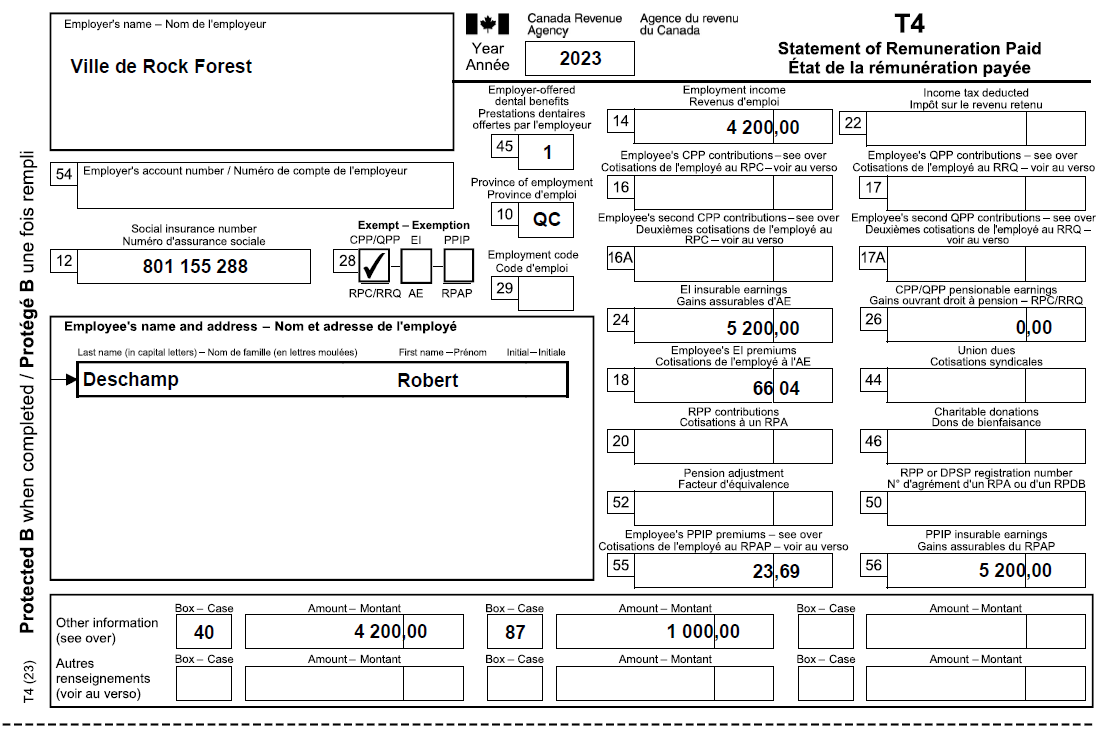
\includegraphics[width=.9\textwidth]{exercice/3-4/Q8/T4.png}
		\caption{Exercice 4, T4}
		\label{fig:chap3Exercice4T4}
	\end{figure}
	\begin{figure}
		\centering
		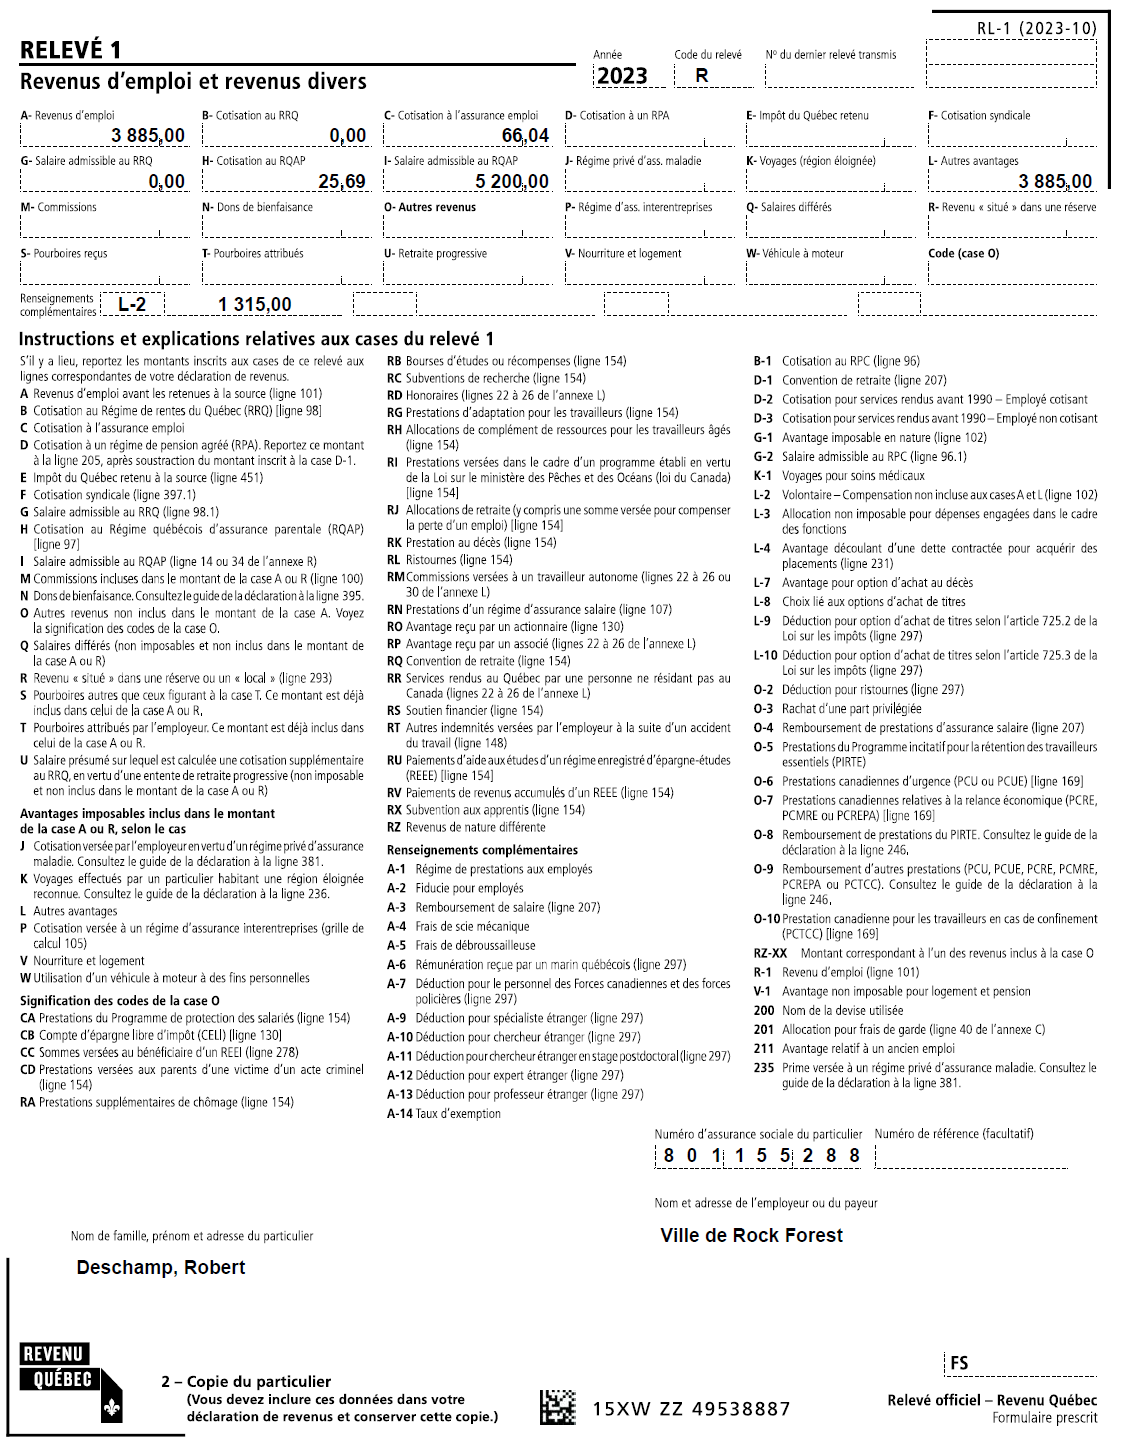
\includegraphics[width=.9\textwidth]{exercice/3-4/Q8/RL1.png}
		\caption{Exercice 4, RL-1}
		\label{fig:chap3Exercice4RL1}
	\end{figure}
	
	Si Robert décide de réclamer le montant pour pompier volontaire, quel montant doit-il inscrire aux lignes 10100 de sa T1 et 101 de sa
	TP-1? Expliquez votre réponse.
\end{question}
Robert doit inscrire \numprint{5200}~\$ à la ligne 10100 de sa T1 et à la ligne 101 de sa TP-1. Un contribuable ne peut bénéficier à la fois de l'exonération d'impôt et du crédit d'impôt pour pompiers volontaires. S'il désire renoncer à l'exemption d'impôt au profit du crédit d'impôt, le montant inscrit à la case 87 du T4 doit être ajouté au montant de la case 14. Au Québec, le montant de la case L-2 du relevé 1 doit être ajouté au montant de la case A.



\section{Prestation universelle pour la garde d'enfants (PUGE)}
\begin{intro}
	Bien que ce programme ne soit plus offert depuis 2016, les dispositions du programme sont toujours valables pour les paiements rétroactifs.
\end{intro}
La \acrfull{puge} était un soutien financier direct, versée par le gouvernement fédéral.


\subsection{Traitement fiscal}
Le total des montants de la PUGE versés durant l'année est inscrit à la case~10 du feuillet RC62. 

Au fédéral, il doit être inscrit à la ligne~11700 de la déclaration T1 de l'époux ou conjoint de fait qui a le revenu net le moins élevé, peu importe celui qui a reçu les versements et le RC62. 

De plus, on doit en reporter le montant dans la partie \og Renseignements sur votre époux ou conjoint de fait », à la page 1 de la déclaration T1 de l'époux ou conjoint de fait ayant le revenu le plus élevé.

Au Québec, le total des versements reçus doit être inscrit à la ligne~278 de la déclaration TP-1 du conjoint au 31 décembre 2023 qui a le revenu net le moins élevé.

Au fédéral comme au Québec, si le revenu net du contribuable et celui de son époux ou conjoint de fait sont égaux, c'est celui qui a reçu les versements qui doit déclarer les montants reçus.

\subsubsection{Famille monoparentale}
Au fédéral, les chefs de famille monoparentale peuvent choisir d'inclure tous les montants de la PUGE qu'ils ont reçus dans le revenu de la personne à charge admissible pour laquelle ils ont demandé le montant.

S'ils font un tel choix, le montant de la case~10 du RC62 entre alors dans le revenu net de la personne pour laquelle ils demandent un montant pour une personne à charge admissible. 

Si cette personne produit une déclaration de revenus, elle doit déclarer le montant à la ligne~11700 de sa déclaration fédérale. Par ailleurs, les chefs de famille monoparentale doivent inscrire le même montant à la ligne~11701 de leur déclaration fédérale, au lieu de la ligne~11700.


\subsection{Remboursement de la prestation universelle pour la garde d'enfants}
Il est possible qu'un contribuable ou son époux ou conjoint de fait ait remboursé en 2023 un revenu de la PUGE qu'il a déclaré dans une année passée. Si c'est le cas, le montant figure à la case~12 du feuillet RC62. Cette personne peut réclamer une déduction correspondant au montant de la case~12 du feuillet RC62, à la ligne~21300 de la déclaration T1 de 2023.

Son époux ou conjoint de fait doit inscrire le montant du remboursement dans la partie \og Renseignements sur votre époux ou conjoint de fait », page 1 de la T1. 

Au Québec, la déduction peut être réclamée à la ligne~297, avec le code \og 24 \fg{} à la case~296, de la TP-1. Aucune autre inscription ne doit être faite sur cette déclaration.



\section{Crédit d'impôt pour nouveau diplômé travaillant dans une région ressource éloignée du Québec}
Le crédit est calculé sur le formulaire TP-776.1.ND Crédit d'impôt pour nouveau diplômé travaillant dans une région ressource éloignée et est réclamé à la ligne~392 de la TP-1.

\qct\href{https://www.revenuquebec.ca/fr/services-en-ligne/formulaires-et-publications/details-courant/tp-776-1-nd/}{Crédit d'impôt pour nouveau diplômé travaillant dans une région ressource éloignée }

Le montant cumulatif de ce crédit d'impôt non remboursable est de \numprint{10000}~\$ pour les nouveaux diplômés titulaires d'un diplôme de niveau postsecondaire (collégial ou universitaire) qui ont commencé à occuper un emploi dans les 24 mois suivants la date à laquelle ils ont complété leur formation ou obtenu leur diplôme.

\begin{note}
	les diplômes d'études professionnels, les attestations de formation professionnelle et les attestations de spécialisation professionnelle décernés par le Ministère de l'Éducation, du Loisir et du Sport ne font pas partie des diplômes reconnus. L'obtention d'un tel diplôme permet encore l'admissibilité au crédit d'impôt cumulatif de \numprint{8000}~\$.
\end{note}



\section{Crédits d'impôt non remboursables}
La partie des crédits d'impôt relatifs à l'emploi n'est qu'une introduction aux nombreux crédits d'impôt à venir.



\section{Frais de déménagement}
Le contribuable qui déménage pour occuper un emploi dans un nouveau lieu peut réclamer des frais de déménagement aux lignes~21900 de la T1 et 228 de la TP-1.


\subsection{Comment faire la réclamation}
Le contribuable doit utiliser les formulaires T1-M au fédéral et TP-348 au Québec.

Il n'est pas nécessaire d'avoir trouvé un emploi au moment du déménagement. Toutefois, la réclamation du contribuable peut être refusée lorsque le but principal du déménagement n'était pas de se trouver un emploi ou qu'il a pris beaucoup de temps avant de s'en trouver un.

Si les deux conjoints déménagent pour occuper de nouveaux emplois ou créer de nouvelles entreprises, les frais de déménagement peuvent être partagés entre eux.

Si un employeur mute un employé à un nouvel endroit et paie une partie ou la totalité des frais de déménagement, ces mêmes frais ne peuvent être déduits par l'employé. Seuls les frais de déménagement admissibles en sus de ceux payés ou payables par l'employeur ou pour lesquels le contribuable n'est pas remboursé sont déductibles.

Un contribuable n'est pas considéré comme ayant changé son lieu de résidence s'il déménage pour une période temporaire et continue de conserver sa résidence pour que sa famille y demeure pendant qu'il est parti.


\subsection{Condition relative à la distance}
La nouvelle résidence doit permettre au particulier de se rapprocher d'au moins 40 kilomètres du nouveau lieu de travail, comparativement à la distance entre l'ancienne résidence et le nouveau lieu de travail.


\subsection{Frais admissibles}
\begin{itemize}[label=\twemoji{check mark button}]
	\item Les frais de transport des effets personnels, y compris l'emballage, le déplacement, l'entreposage et les assurances;
	\item Les frais de déplacement vers la nouvelle résidence pour le contribuable et sa famille, y compris les frais de voyage, de repas et de logement pendant le trajet;
	\item Les frais de subsistance (repas et logement) pour le contribuable et les membres de sa famille pour séjourner à proximité de l'ancienne et/ou de la nouvelle résidence (période maximale de 15 jours);
	\item Les frais de résiliation du bail à l'ancienne résidence, à l'exclusion de tout loyer payé pendant qu'il y demeurait;
	\item Les frais accessoires consécutifs au déménagement, y compris le coût de la révision des documents juridiques pour tenir compte du changement d'adresse, le coût du remplacement des permis de conduire et des certificats d'immatriculation des véhicules non commerciaux (sauf les assurances) et les frais de branchement et de débranchement exigés par les services publics;
	\item Les frais d'entretien de l'ancienne résidence si elle est demeurée vacante et que des efforts ont été faits en vue de la vendre, y compris les intérêts hypothécaires, impôts fonciers, primes d'assurance, chauffage, électricité et les services publics, jusqu'à l'occurrence de \numprint{5000}~\$;
	\item Les frais relatifs à la vente de l'ancienne résidence, y compris la pénalité pour l'acquittement d'une hypothèque avant l'échéance, la commission versée à l'agent immobilier, les honoraires payés au notaire ou à l'avocat, les frais de publicité, les frais d'arpentage, etc.; 
	\item Les frais relatifs à l'acquisition de la nouvelle résidence, seulement si l'ancienne résidence a été vendue suite au déménagement (frais juridiques, droits de mutation (taxe municipale de bienvenue), enregistrement du droit de propriété au Bureau de la publicité des droits). Si c'est une première maison, ces frais ne sont pas admissibles.
\end{itemize}


\subsection{Frais de déménagement non déductibles}
\begin{itemize}[label=\twemoji{cross mark}]
	\item Les frais de transport engagés avant le déménagement pour la recherche d'un emploi, d'une résidence au nouvel endroit ou pour tout autre motif;
	\item Le coût des travaux effectués pour faciliter la vente de l'ancienne résidence et les pertes subies lors de la vente;
	\item La valeur des articles que les déménageurs refusent de prendre (plantes, aliments surgelés, munitions, peinture, carburant, huile, produits de nettoyage);
	\item Les frais qui ont été payés pour nettoyer ou réparer une résidence louée afin de respecter les exigences du propriétaire ou pour remplacer des biens à usage personnel (remise, bois de chauffage, rideaux, moquettes);
	\item Le coût de l'acheminement du courrier à la nouvelle adresse;
	\item Le coût des transformateurs et adaptateurs pour les appareils électroménagers;
	\item Les frais d'inspection de véhicules et le test d'émission; 
	\item Les frais de vente de l'ancienne résidence, si le contribuable en a retardé la mise en vente pour des raisons d'investissement ou de meilleures conditions de vente.
\end{itemize}


\subsection{Calcul des frais de déplacement et des frais de repas lors de l'hébergement temporaire}
Le contribuable a le choix entre deux méthodes (simplifiée ou détaillée) pour calculer les dépenses pouvant être réclamées pour les frais de repas et les frais de déplacement de l'ancienne résidence à la nouvelle résidence. Revenu Québec utilise les mêmes taux pour la méthode simplifiée que l'ARC.

\subsubsection{Calcul des frais de repas}

\paragraph{Méthode simplifiée}
Le contribuable qui choisit la méthode simplifiée peut réclamer un montant fixe de 23~\$ par repas, par personne, jusqu'à un maximum de 69~\$ par jour sans avoir à produire de reçus. 

La méthode simplifiée peut être utilisée pour les repas consommés pendant le trajet vers le nouveau lieu de résidence et pendant la période maximale de 15 jours pour le séjour dans un logement temporaire. 

Le contribuable doit être en mesure de fournir des pièces justificatives pour établir la durée de location du logement.

\paragraph{Méthode détaillée}
Selon cette méthode, un contribuable peut réclamer les frais de repas qu'il a payés, en fonction de ses reçus (à coût raisonnable), qu'il doit conserver.

\subsubsection{Calcul des frais de kilométrage}
Le contribuable qui utilise sa voiture personnelle peut choisir la méthode simplifiée ou la méthode détaillée pour calculer les frais de véhicule.

\begin{note}
	Le contribuable n'a aucune obligation de choisir la même méthode pour le calcul des frais de repas et de kilométrage. Il est tout à fait possible de choisir une méthode pour réclamer les frais de repas et l'autre méthode pour les frais de kilométrage.
\end{note}

\paragraph{Méthode simplifiée}
Le contribuable peut réclamer les dépenses relatives à son véhicule en utilisant un taux par kilomètre parcouru. Pour le Québec, le taux de 2023 est de 0,575~\$ par kilomètre parcouru.

Le taux en question varie selon la province ou le territoire d'où provient le déménagement. Par conséquent, les déménagements à l'intérieur du Québec seraient à un taux de 0,575~\$ par kilomètre, tandis qu'un déménagement en provenance de l'Ontario serait à un taux de 0,59~\$ par kilomètre.

Bien que le contribuable qui utilise la méthode simplifiée ne soit pas obligé de conserver des reçus, il doit toutefois conserver un registre du kilométrage parcouru relativement au déménagement.

\paragraph{Méthode détaillée}
Le contribuable peut utiliser cette méthode pour réclamer les frais de fonctionnement et les frais de propriété d'une automobile utilisée à des fins de déménagement (pourcentage d'utilisation du véhicule à des fins du déménagement). Il doit tenir un registre du kilométrage parcouru et conserver tous ses reçus.

Les frais de fonctionnement incluent l'essence, l'huile, les pneus, l'immatriculation, les primes d'assurance, l'entretien et les réparations du véhicule. Les frais de propriété du véhicule comprennent les taxes, les intérêts sur emprunt pour financer son achat et l'amortissement. 

\subsection{Limite du revenu admissible net}
Les frais de déménagement peuvent être déduits seulement du revenu net gagné au nouveau lieu de travail. 

Pour déterminer le revenu net admissible au nouveau travail, le contribuable doit d'abord calculer le total des revenus gagnés au nouveau lieu de travail comme suit:
\begin{itemize}
	\item Le montant inscrit sur le feuillet T4 relié au nouveau lieu de travail et déclaré à la ligne~10100. La même condition s'applique pour le relevé~1 et le montant est déclaré à la ligne~101 de la TP-1; plus
	\item Le revenu d'emploi gagné sur le feuillet T4A et déclaré à la ligne~10400. La même condition s'applique pour le relevé~1 et le montant est déclaré à la ligne~107 de la TP-1; plus
	\item Le revenu net d'entreprise si travailleur autonome; plus
	\item Les prestations du Programme de protection des salariés.
\end{itemize}

Par la suite, le contribuable doit réduire le total de ces montants en utilisant les déductions admissibles suivantes qu'il réclame:
\begin{itemize}
	\item Au Québec seulement, la déduction pour travailleur (ligne~201);
	\item La cotisation versée à un RPA reliée au nouvel emploi aux cases~20 du T4 et D du relevé~1 (lignes~20700 de la T1 et 205 de la TP-1);
	\item Au fédéral, la cotisation syndicale, professionnelle ou semblable reliée au nouvel emploi (ligne~21200 de la T1);
	\item Tous les autres frais admissibles reliés au nouveau lieu de travail, habituellement inscrits aux lignes~22215, 22900, 23100 et 23200 de la T1 et aux lignes~207, 236, 248 et 250 de la TP-1.
\end{itemize}

\begin{note}
	Les déductions pour les travailleurs (ligne~201) et les cotisations bonifiées au RPC/RRQ (lignes~22215 et ligne~248) sont calculées en fonction du revenu gagné total, provenant à la fois de l'emploi à l'ancien et au nouvel emplacement. 
	
	Par conséquent, un prorata de ces montants doit être calculé. 
	
	Utilisez la valeur du revenu gagné au nouvel emplacement / le revenu gagné total.
\end{note}

Par ailleurs, le calcul du revenu net au nouveau lieu de travail n'est pas nécessaire si le revenu brut à cet endroit est substantiellement plus élevé que les frais de déménagement. Dans une telle situation, il suffit d'entrer le  montant des revenus d'emplois des lignes~10100 et 10400 de la T1 et ceux des lignes~101 et 107 de la TP-1, plus les prestations du Programme de protection des salariés aux lignes~10400 de la T1 et 154 de la TP-1, sur les déclarations appropriées.


\subsection{Réclamation des frais de déménagement}
Au fédéral, le contribuable doit utiliser le formulaire T1-M afin de calculer et réclamer la déduction pour frais de déménagement à la ligne~21900 de la T1. Il doit le conserver, ainsi que les reçus et les autres pièces justificatives, afin de pouvoir les fournir à l'ARC sur demande.

Au Québec, le contribuable doit compléter le formulaire TP-348 et réclamer la déduction à la ligne~228 de la TP-1. Il doit joindre le formulaire à sa déclaration provinciale. Il doit conserver les reçus relatifs aux frais qu'il réclame pour pouvoir les fournir sur demande.


\subsection{Report des frais de déménagement inutilisés d'une année précédente}
Il arrive que le revenu net gagné au nouveau lieu de travail soit inférieur au frais de déménagement. Cette situation peut se produire lorsque le contribuable déménage vers la fin de l'année. En raison de la limite du revenu net au nouveau lieu de travail, il ne pourra pas réclamer tous ses frais dans l'année du déménagement. Ces frais inutilisés peuvent alors être reportés et utilisés pour réduire son revenu gagné au même lieu de travail l'année suivante.

Au fédéral, lorsqu'il peut réclamer les frais inutilisés d'une année précédente, le contribuable ne doit pas compléter un autre formulaire T1-M. Il doit plutôt indiquer, à la ligne~21900 de la T1, le montant du report. 

Au Québec, le contribuable doit inscrire l'année du déménagement à la gauche de la case~Indiquant l'année d'imposition (vis-à-vis la partie 1 \og Renseignements sur l'identité »). Compléter la partie 1. Inscrire le montant reporté de l'année précédente à la ligne~18 et remplir les lignes~19 à 24.


\subsection{Déménagements multiples}
Si le contribuable a reporté des dépenses puis déménage à nouveau pour trouver un autre emploi, les dépenses non utilisées du premier déménagement sont perdues; elles ne peuvent pas être réutilisées. Pour le deuxième déménagement, le contribuable peut utiliser seulement les dépenses du deuxième déménagement sur le revenu du deuxième emploi.

\cat\href{https://www.canada.ca/fr/agence-revenu/services/formulaires-publications/formulaires/t1-m.html}{T1-M Déduction pour frais de déménagement}

\qct\href{https://www.revenuquebec.ca/fr/services-en-ligne/formulaires-et-publications/details-courant/tp-348/}{Frais de déménagement}



\section{Exercice 5}
\setcounter{question}{0}
\begin{question}
	Thomas vivait à 50 km de son nouvel emploi. Juste avant de commencé son nouvel emploi, il a déménagé dans une nouvelle résidence située à 12 km de son nouveau lieu de travail.
	
	Peut-il déduire ses frais de déménagement? Expliquez votre réponse.
\end{question}
Non. Alors qu'il habitait auparavant à 50 kilomètres de son nouveau lieu de travail, la proximité entre sa nouvelle résidence et son lieu de travail réduit la distance à 12 kilomètres. Il n'a déménagé que de 38 kilomètres de son ancienne résidence (moins des 40 kilomètres requis) pour se rapprocher de son nouveau lieu de travail.

\begin{question}
	Simon est sans emploi depuis deux mois. Il a appris qu'il y avait des opportunités d'emploi dans une autre province située à 800 km de chez lui. Il a donc décidé de déménager dans cette province et de tenter sa chance.
	
	Peut-il réclamer ses frais de déménagement? Expliquez votre réponse.
\end{question}
Oui. Selon les lignes directrices administratives de l'ARC, il n'est pas nécessaire qu'un contribuable ait un emploi avant le déménagement. Il est seulement nécessaire que le déménagement soit lié à l'emploi.

Si Simon ne trouve pas d'emploi avant la fin de l'année d'imposition suivant le déménagement, il ne pourra pas demander de déduction pour cette année d'imposition, mais il pourra reporter le montant.

Toutefois, la demande de Simon peut être rejetée si l'objectif principal du déménagement n'était pas de trouver un emploi ou s'il met trop de temps à trouver un emploi après avoir déménagé.

\begin{question}
	Renée peut réclamer des frais de déménagement dans l'année. Son revenu net de son nouvel emploi s'élève à \numprint{3800}~\$ et ses frais de déménagement admissibles sont de \numprint{4200}~\$. 
\end{question}
\setcounter{sousQuestion}{0}
\begin{sousQuestion}
	Quel montant peut-elle réclamer aux lignes~21900 de la T1 et 228 de la TP-1?
\end{sousQuestion}
Un maximum de \numprint{3800}~\$. Il convient de tenir compte de toute déduction appliquée avant le calcul du revenu net.
\begin{sousQuestion}
	Que peut-elle faire avec l'excédent?
\end{sousQuestion}
Les 400~\$ restants peuvent être reportés à l'année suivante et déduits du revenu net au nouveau lieu de travail.

\begin{question}
	En supposant que toutes les autres conditions sont remplies, indiquez pour chacune des dépenses de déménagement suivantes celles qui sont:
	\begin{enumerate}[label=\Alph*.]
		\item Déductibles au complet;
		\item Déductibles à certaines conditions;
		\item Non déductibles.
	\end{enumerate}
\end{question}
\setcounter{sousQuestion}{0}
\begin{sousQuestion}
	Perte sur la vente d'une résidence.
\end{sousQuestion}
C. Non déductible.

\begin{sousQuestion}
	Emballage et autres coûts relatifs au déménagement.
\end{sousQuestion}
A. Déductibles au complet.

\begin{sousQuestion}
	Déplacements avant le déménagement pour la recherche d'un emploi ainsi que d'une résidence.
\end{sousQuestion}
C.  Non déductibles.

\begin{sousQuestion}
	Résiliation du bail pour location de l'ancienne résidence.
\end{sousQuestion}
A.  Déductibles au complet

\begin{sousQuestion}
	Repas et hébergement pendant le trajet vers la nouvelle résidence.
\end{sousQuestion}
A.  Déductibles au complet

\begin{sousQuestion}
	Frais juridiques relatifs à l'achat de la nouvelle résidence, incluant les taxes de mutation immobilière. 
\end{sousQuestion}
B.  Déductibles à certaines conditions. Notez que ces frais sont admissibles seulement si l'ancienne résidence a été vendue suite au déménagement. En d'autres mots, si le contribuable était locataire avant le déménagement, ces frais ne sont pas admissibles.

\begin{sousQuestion}
	Réparations nécessaires afin de rendre l'ancienne résidence plus attrayante en vue de la vente.
\end{sousQuestion}
C.  Non déductibles.

\begin{sousQuestion}
	Frais relatifs à la vente de l'ancienne résidence.
\end{sousQuestion}
A.  Déductibles au complet

\begin{sousQuestion}
	Frais de branchement des services publics à la nouvelle résidence.
\end{sousQuestion}
A.  Déductibles au complet

\begin{sousQuestion}
	Repas et logement temporaire situé à proximité de l'ancienne ou de la nouvelle résidence.
\end{sousQuestion}
B.  Déductibles à certaines conditions. Ces frais sont admissibles pour une période maximale de 15 jours.

\begin{sousQuestion}
	Frais d'entretien de l'ancienne résidence après le déménagement.
\end{sousQuestion}
B.  Déductibles à certaines conditions. Les frais suivants sont admissibles jusqu'à concurrence de \numprint{5000}~\$ seulement si l'ancienne résidence est demeurée vacante et que des efforts ont été faits en vue de la  vendre: intérêts hypothécaires, impôts fonciers, primes d'assurance, chauffage, électricité et les services publics relativement à l'ancienne résidence.

\begin{sousQuestion}
	Perte de salaire due au déménagement.
\end{sousQuestion}
C.  Non déductibles

\begin{question}
	Le 28 octobre 2023, Paul Grégoire, NAS 800 000 986, a quitté l'appartement qu'il occupait à Montréal  pour déménager à Québec. Il a quitté son emploi de Montréal pour occuper un emploi à Québec où il a commencé à travailler le 2 novembre. Il réside maintenant à 3 km de son nouveau lieu de travail, tandis que son ancienne résidence est à 250 km de son nouveau lieu de travail, cf. table~\ref{table:chap3Exercice5Adresses}
	\begin{table}
		\centering
		\begin{tabular}{|l|l|}
			\hline
			\multicolumn{2}{|c|}{\textbf{Ancienne adresse de Paul Grégoire}} \\ \hline
			Numéro et rue                  & 5502 rue St-Denis               \\ \hline
			Ville, province et code postal & Montréal, QC, H2Y 3V9           \\ \hline
			\multicolumn{2}{|c|}{\textbf{Ancien emploi}}                     \\ \hline
			Nom de la société              & St-Laurent Électronique         \\ \hline
			Numéro et rue                  & 2500 rue Papineau               \\ \hline
			Ville, province et code postal & Montréal, QC, H1S 2X7           \\ \hline
			\multicolumn{2}{|c|}{\textbf{Nouvelle adresse de Paul Grégoire}} \\ \hline
			Numéro et rue                  & 120 rue St-Cyrille Est          \\ \hline
			Ville, province et code postal & Québec, QC, G2L 3L4             \\ \hline
			\multicolumn{2}{|c|}{\textbf{Nouvel emploi}}                     \\ \hline
			Nom de la société              & Transports Québec               \\ \hline
			Numéro et rue                  & 15800 boulevard Henri-Bourassa  \\ \hline
			Ville, province et code postal & Québec, QC, G2G 3L4             \\ \hline
		\end{tabular}
		\caption{Exercice 5, ancienne et nouvelle adresse}
		\label{table:chap3Exercice5Adresses}
	\end{table}
	
	Paul a loué les services d'un déménageur et a fait le voyage en auto avec son épouse et leurs trois enfants. Avant de s'installer dans son logement, la famille a hébergé dans une auberge, cf. table~\ref{table:chap3Exercice5FraisDemenagement}
	\begin{table}
		\centering
		\begin{tabular}{|l|r|}
			\hline
			\multicolumn{2}{|c|}{\textbf{Frais de déménagement}} \\ \hline
			Compagnie de déménagement      &  Déménagements Côté \\ \hline
			Coût du déménagement           &  \numprint{1225}~\$ \\ \hline
			\multicolumn{2}{|c|}{\textbf{Durant le trajet}}      \\ \hline
			Frais du voyage de 250 km      &              125~\$ \\ \hline
			Frais de repas pour la famille &               57~\$ \\ \hline
			\multicolumn{2}{|c|}{\textbf{À l'arrivée}}           \\ \hline
			13 nuits à l'Auberge Neptune   &      92~\$ par nuit \\ \hline
			13 jours de repas              &  \numprint{2215}~\$ \\ \hline
		\end{tabular}
		\caption{Exercice 5, frais de déménagement}
		\label{table:chap3Exercice5FraisDemenagement}
	\end{table}
	
	Infos supplémentaires:
	\begin{itemize}
		\item 	Durant l'année d'imposition, les dépenses d'automobile de Paul se sont élevées à \numprint{9000}~\$ et il a parcouru un total de \numprint{20000}~kilomètres.
		\item 	Paul a payé 350~\$ pour résilier le bail de son logement de Montréal.
	\end{itemize}
	
	Voici les T4 et le RL-1 de chaque emploi de Paul Grégoire: table~\ref{table:chap3Exercice5T4RL1}.
	\begin{table}
		\centering
		\begin{tabular}{|c|r|c|r|}
			\hline
			\multicolumn{4}{|c|}{\cellcolor{lightgray}St-Laurent Électronique - Ancien emploi} \\ \hline
			\multicolumn{2}{|c|}{\textbf{T4}}      &  \multicolumn{2}{c|}{\textbf{relevé~1}}   \\ \hline
			\textbf{Case} &       \textbf{Montant} & \textbf{Case} &          \textbf{Montant} \\ \hline
			     14       & \numprint{39600,00}~\$ &       A       &    \numprint{39600,00}~\$ \\ \hline
			     17       &  \numprint{2310,40}~\$ &       B       &     \numprint{2310,40}~\$ \\ \hline
			     18       &              502,92~\$ &       C       &                 502,92~\$ \\ \hline
			     44       &              200,00~\$ &       F       &                 200,00~\$ \\ \hline
			     55       &              195,62~\$ &       G       &                 195,62~\$ \\ \hline\hline
			\multicolumn{4}{|c|}{\cellcolor{lightgray}Transports Québec - Nouvel emploi}       \\ \hline
			\multicolumn{2}{|c|}{\textbf{T4}}      &  \multicolumn{2}{c|}{\textbf{relevé~1}}   \\ \hline
			\textbf{Case} &       \textbf{Montant} & \textbf{Case} &          \textbf{Montant} \\ \hline
			     14       &  \numprint{9370,00}~\$ &       A       &     \numprint{9370,00}~\$ \\ \hline
			     17       &              375,68~\$ &       B       &                 375,68~\$ \\ \hline
			     18       &              119,00~\$ &       C       &                 119,00~\$ \\ \hline
			     18       &              880,00~\$ &       C       &                 880,00~\$ \\ \hline
			     44       &               40,00~\$ &       F       &                  40,00~\$ \\ \hline
			     55       &               46,29~\$ &       G       &                  46,29~\$ \\ \hline
		\end{tabular}
		\caption{Exercice 5, T4 et RL-1}
		\label{table:chap3Exercice5T4RL1}
	\end{table}
	
	Le montant de la déduction pour la cotisation bonifiée au RRQ du nouvel emploi de Paul est de 87,00~\$, calculé comme suit:
	\begin{enumerate}
		\item Calculer le prorata de l'exemption:
		\[ \frac{\numprint{9370}~\$}{\numprint{9370}~\$ + \numprint{39600}~\$} \times \numprint{3500}~\$ = 669,70~\$ \]
		\item 	Calculer la déduction:
		\[ (\numprint{9370,00}~\$ - 669,70~\$) \times 1,00~\% = 87,00~\$ \]
	\end{enumerate}
	
	Transport Québec n'a remboursé aucun frais de déménagement.
	
	Préparez les réclamations fédérale et provinciale relatives aux frais de déménagement de Paul à l'aide des formulaires \href{https://www.canada.ca/fr/agence-revenu/services/formulaires-publications/formulaires/t1-m.html}{T1-M} (pages 4, 5 et 6) et \href{https://www.revenuquebec.ca/fr/services-en-ligne/formulaires-et-publications/details-courant/tp-348/}{TP-348} (pages 1 et 2).
\end{question}

Choix de la méthode simplifiée ou de la méthode détaillée pour réclamer les frais de repas et les dépenses d'automobile: table~\ref{table:chap3Exercice5MethodeSimplifieeDetaillee}
\begin{table}
	\centering
	\begin{tabular}{|c|r|r|}
		\hline
		&
		Méthode simplifiée &
		Méthode détaillée \\
		\hline
		
		Repas durant &
		\( 23~\$ \times 5 \times 1 \times 1~\text{jour} = 115,00~\$ \) &
		57,00~\$ \\
		
		le trajet &
		&
		\\
		\hline
		
		Repas à l'arrivée &
		\( 23~\$ \times 5 \times 3 \times 13~\text{jours} = \numprint{4485,00}~\$ \) &
		\numprint{2215,00}~\$ \\
		\hline
		
		Automobile &
		\( 250~\text{km} \times 57,5~\text{cents} = 143,75~\$ \) &
		\( \numprint{9000}~\$ \times \frac{250~\text{km}}{\numprint{20000}~\text{km}} = 112,50~\$ \) \\
		\hline
	\end{tabular}
	\caption{Exercice 5, méthode simplifiée et détaillée}
	\label{table:chap3Exercice5MethodeSimplifieeDetaillee}
\end{table}

Il est donc plus avantageux pour Paul d'utiliser la méthode simplifiée pour les frais de repas et pour les dépenses d'automobile.

Pour déterminer le revenu net du nouvel emploi, il faut calculer les points suivants:
\begin{itemize}
	\item \textbf{Au fédéral:}
	\begin{itemize}
		\item Revenu brut de la case 14 = \numprint{9370}~\$;  moins
		\item RPA de la case 20 = 880~\$;  moins
		\item Cotisation syndicale de la case~44 = 40~\$;  moins
		\item Cotisation bonifiée du RRQ de 87~\$. 
		\item \textbf{Résultat:} \[ \numprint{9370}~\$~–~880~\$~–~40~\$~-~87~\$ = \numprint{8 363}~\$ \]
	\end{itemize}
	\item \textbf{Au Québec:}
	\begin{itemize}
		\item Revenu brut de la case~A = \numprint{9370}~\$;  moins
		\item Déduction pour travailleur de 251,61~\$\footnote{Il faut établir au prorata la déduction pour travailleur de la ligne~201 de la TP1. Par conséquent, multiplier le montant de \numprint{1315}~\$ au prorata des cases~A, soit \[ \frac{\numprint{9370}~\$}{\numprint{9370}~\$ + \numprint{39600}~\$} \]};  moins                                                                                                                               
		\item RPA de la case 20 = 880~\$;  moins
		\item Déduction pour cotisation au RRQ de 87~\$. 
		\item \textbf{Résultat:} \[ \numprint{9370}~\$~–~251,61~\$~-~880~\$~-~87~\$ = \numprint{8151,39}~\$ \]
	\end{itemize}
\end{itemize}

T1-M : figures~\ref{fig:chap3Exercice5T1M4} à \ref{fig:chap3Exercice5T1M6}.
\begin{figure}
	\centering
	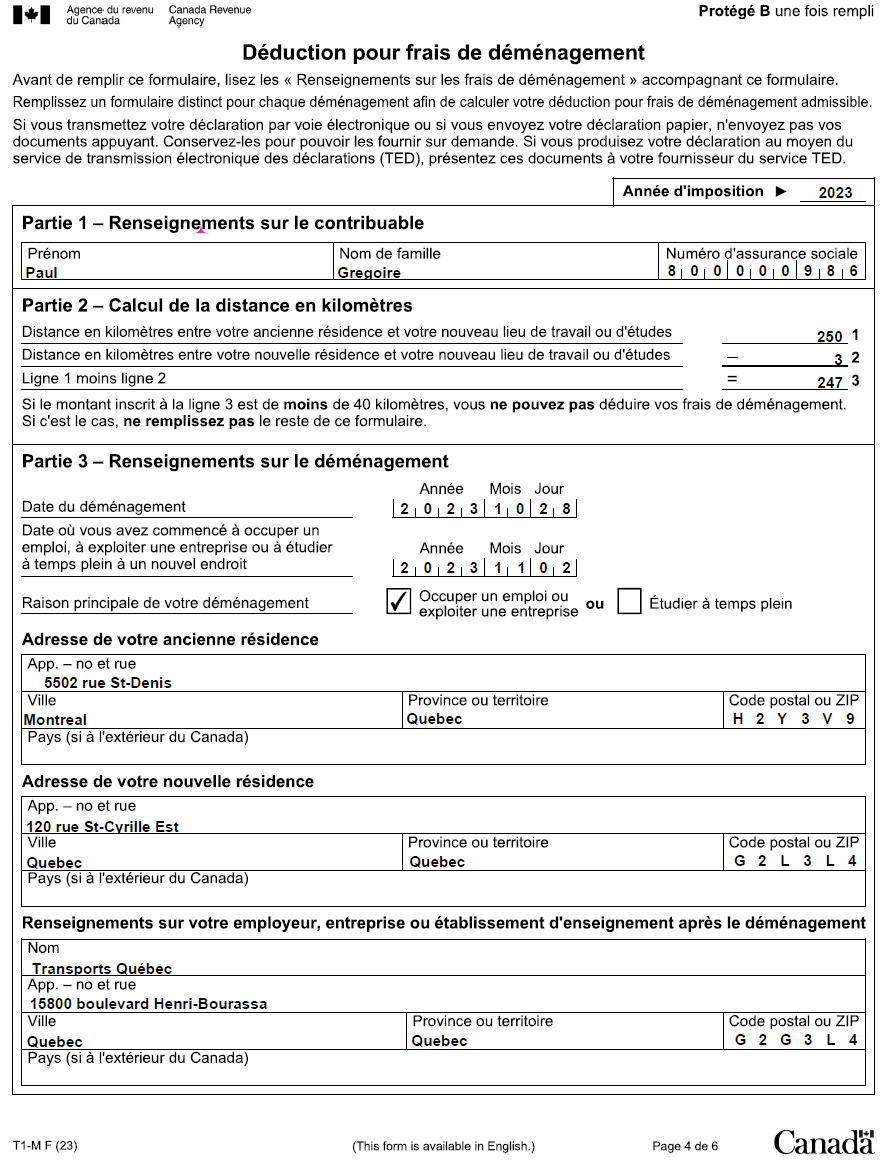
\includegraphics[width=.9\textwidth]{exercice/3-5/Q5/T1-M-p4.png}
	\caption{Exercice 5, T1-M, page 4}
	\label{fig:chap3Exercice5T1M4}
\end{figure}
\begin{figure}
	\centering
	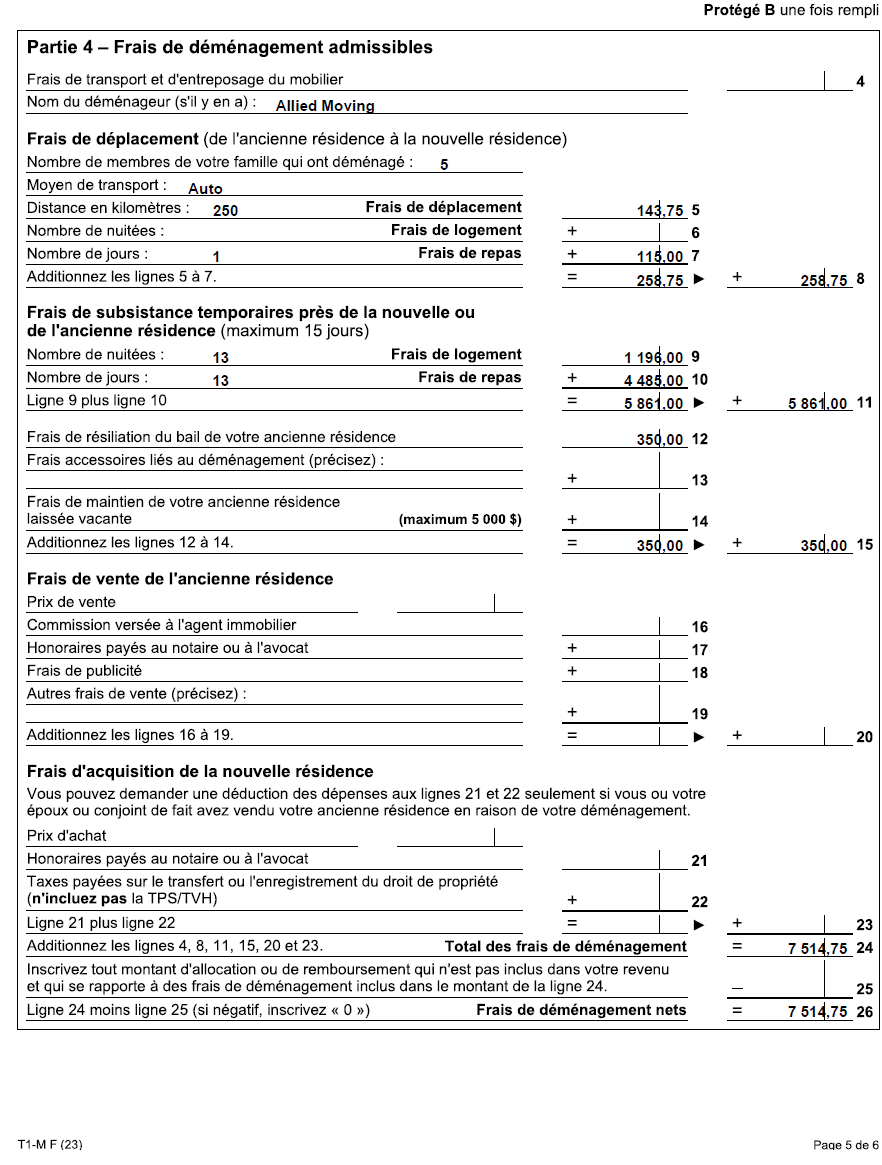
\includegraphics[width=.9\textwidth]{exercice/3-5/Q5/T1-M-p5.png}
	\caption{Exercice 5, T1-M, page 5}
	\label{fig:chap3Exercice5T1M5}
\end{figure}
\begin{figure}
	\centering
	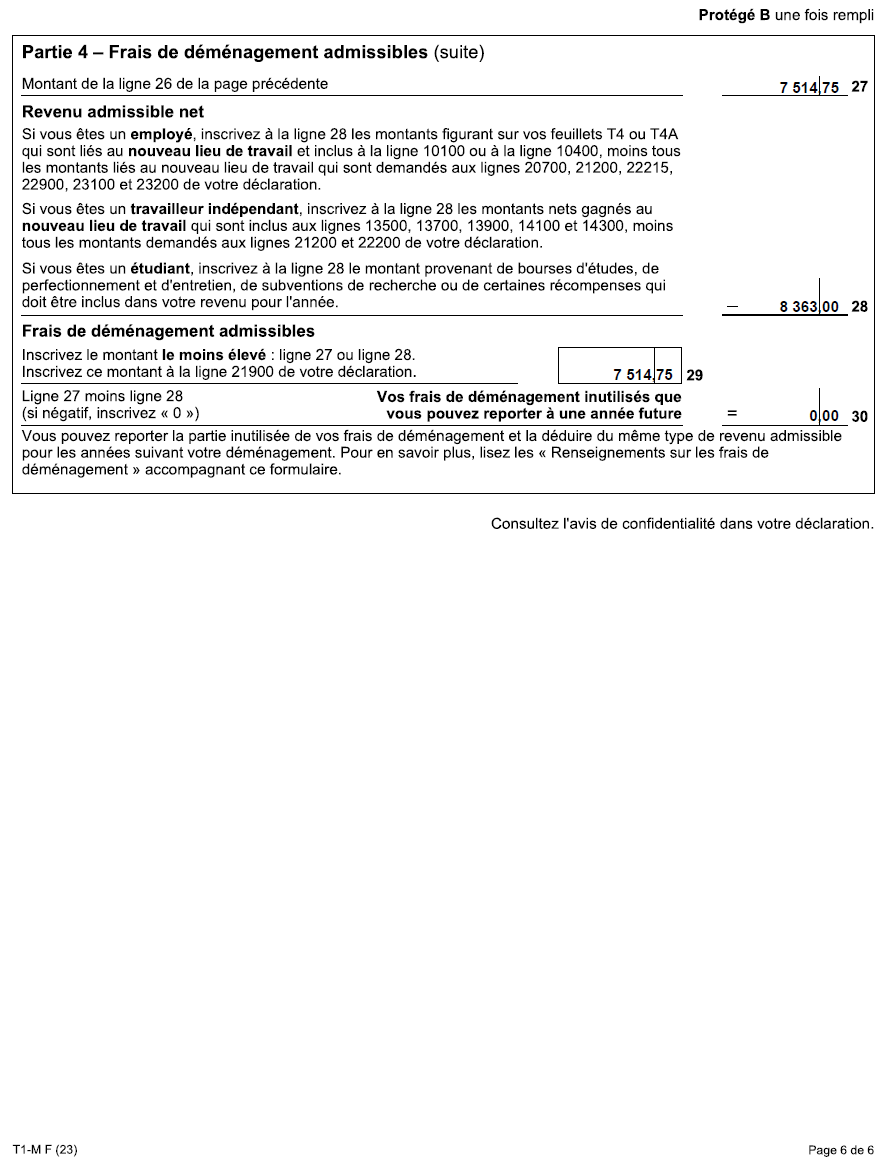
\includegraphics[width=.9\textwidth]{exercice/3-5/Q5/T1-M-p6.png}
	\caption{Exercice 5, T1-M, page 6}
	\label{fig:chap3Exercice5T1M6}
\end{figure}

TP-348: figures \ref{fig:chap3Exercice5TP3481} et \ref{fig:chap3Exercice5TP3482}.
\begin{figure}
	\centering
	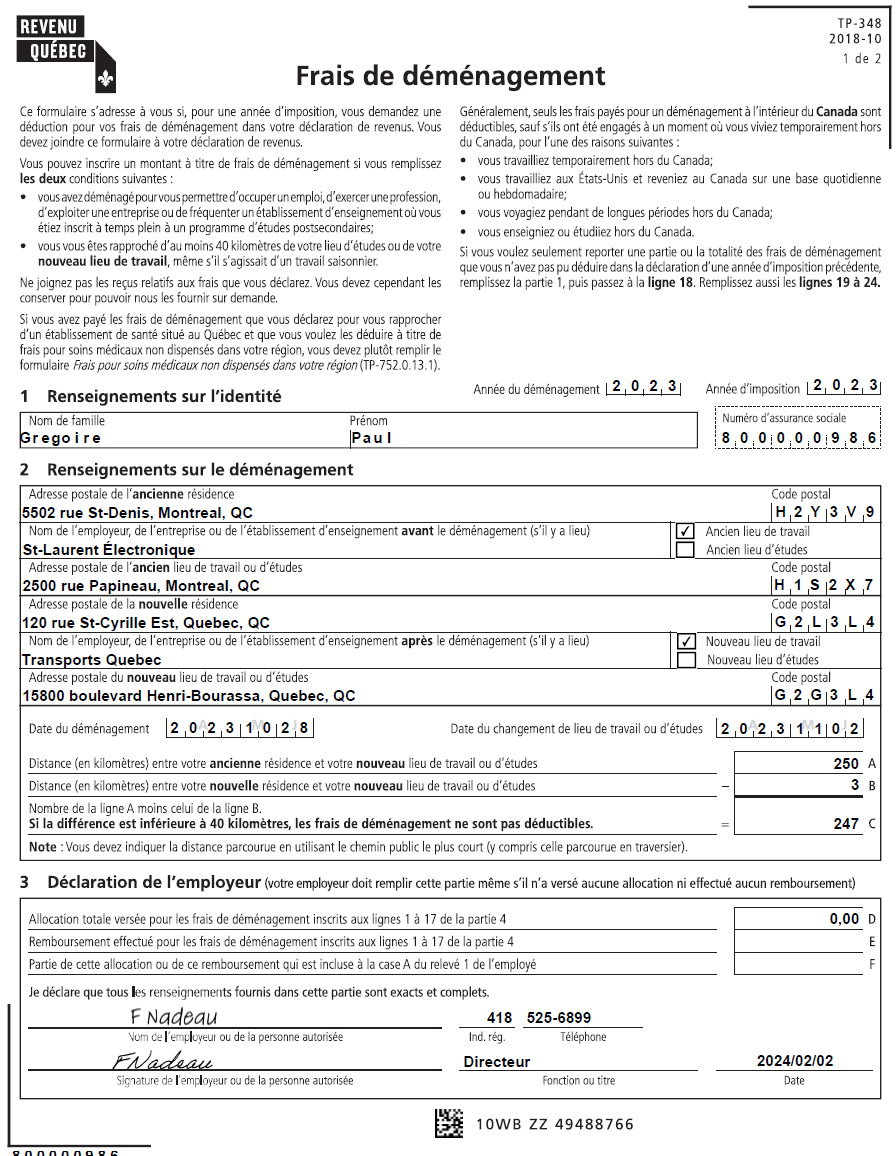
\includegraphics[width=.9\textwidth]{exercice/3-5/Q5/TP-348-p1.png}
	\caption{Exercice 5, TP-348, page 1}
	\label{fig:chap3Exercice5TP3481}
\end{figure}
\begin{figure}
	\centering
	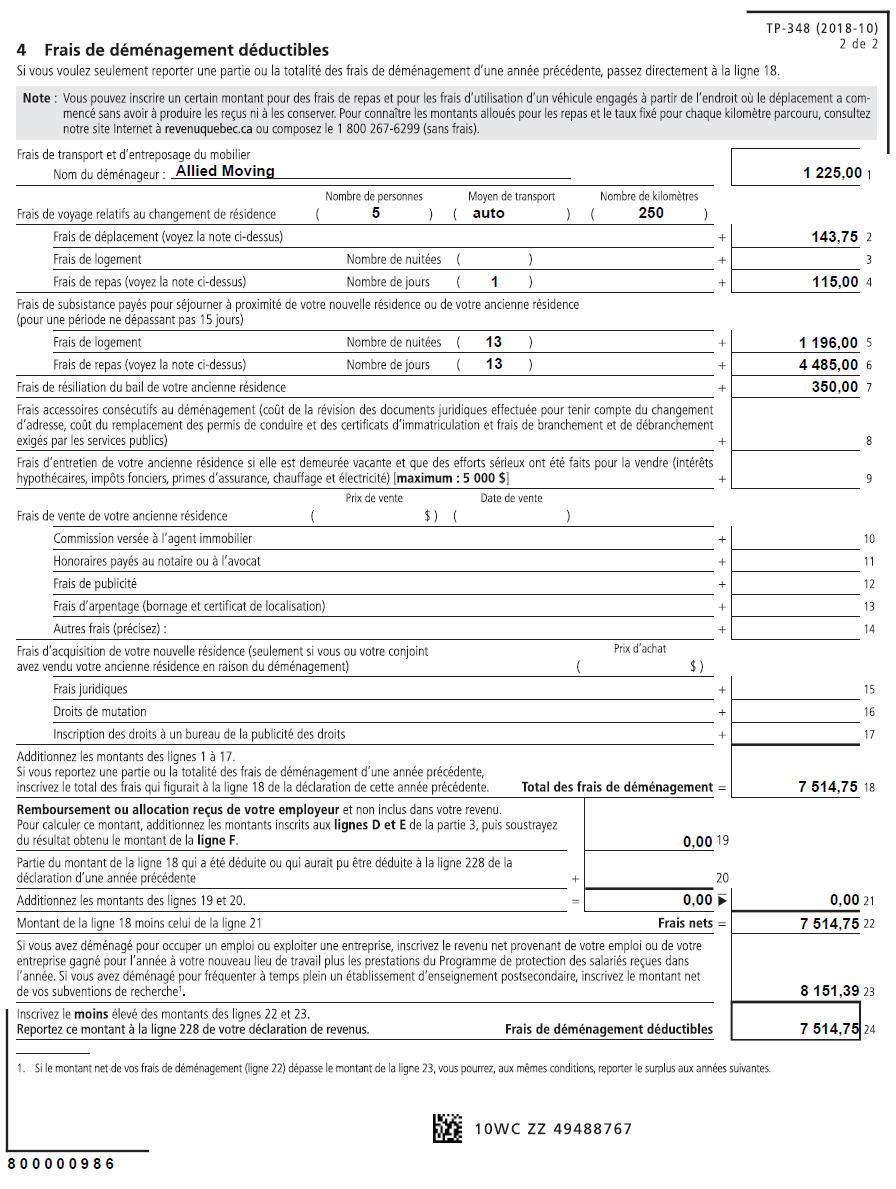
\includegraphics[width=.9\textwidth]{exercice/3-5/Q5/TP-348-p2.png}
	\caption{Exercice 5, TP-348, page 2}
	\label{fig:chap3Exercice5TP3482}
\end{figure}



\section{Sommaire du chapitre 3}
\begin{itemize}
	\item La distinction entre une déduction et un crédit d'impôt.
	\item La \og Déduction pour travailleur \fg{} au Québec seulement.
	\item Les régimes de retraite des gouvernements - RPA et RVÉR.
	\item La complexité du calcul des cotisations syndicales et professionnelles.
	\item L'admissibilité des frais de déménagement.
	\item Le remboursement de salaire et de prestation.
	\item L'impact des déductions spécifiques sur le revenu net.
	\item Un petit aperçu des déductions spécifiques.
	\item L'impact des déductions spécifiques sur le revenu imposable.
	\item Montant de l'impôt à payer.
	\item L'utilisation des crédits d'impôt principalement au fédéral.
	\item Les cotisations aux programmes sociaux (RRQ, AE et RQAP).
	\item Le \og Montant canadien pou emploi \fg{} au fédéral seulement.
	\item Les crédits d'impôt prévus pour les volontaires des services d'urgence.
	\item Les crédits d'impôt pour les nouveaux diplômés travaillant dans les régions ressources éloignées du Québec.
\end{itemize}



\section{Problème de révision du chapitre 3}
\subsection{Renseignements personnels du couple}
Voir la table \ref{table:chapitre3ProblemeRenseignementsPersonnelsCouple}.
\begin{table}
	\centering
	\begin{tabular}{|l|c|c|}
		\hline
		\rowcolor{LightGreen} \textbf{Description} & \textbf{Contribuable 1} & \textbf{Contribuable 2}  \\ \hline
		Nom                                        &    Donna St-Laurent     &     Ginette Bernard      \\ \hline
		NAS                                        &       801 115 296       &       801 115 304        \\ \hline
		Date de naissance                          &      10 avril 1991      &       24 mars 1991       \\ \hline
		Statut civil                               &       \multicolumn{2}{c|}{Conjoints de fait}       \\ \hline
		Sexe                                       &            F            &            F             \\ \hline
		Province de résidence                      &           QC            &            QC            \\ \hline
		Langue                                     &            F            &            F             \\ \hline
		Téléphone                                  &        \multicolumn{2}{c|}{(514) 737-2899}         \\ \hline
		Adresse courriel                           & \multicolumn{2}{c|}{donna.st-laurent@videotron.ca} \\ \hline
		Consentement à l'envoi de communications   &           Oui           &           Oui            \\
		par voie électronique uniquement           &                         &                          \\ \hline
		Régime d'assurance médicaments             &          RAMQ           &           RAMQ           \\ \hline
		Adresse                                    &    \multicolumn{2}{c|}{1896 avenue Des Chênes,}    \\
		                                           &           \multicolumn{2}{c|}{appt 505,}           \\
		                                           &     \multicolumn{2}{c|}{Montréal, QC, H2L 4J8}     \\ \hline
		Citoyenneté canadienne                     &           Oui           &           Oui            \\ \hline
		Élections Canada                           &           Oui           &           Oui            \\ \hline
		Biens étrangers                            &           Non           &           Non            \\ \hline
		Revenu                                     &           Oui           &           Non            \\ \hline
	\end{tabular}
	\caption{Problème, renseignements personnels du couple}
	\label{table:chapitre3ProblemeRenseignementsPersonnelsCouple}
\end{table}



\subsection{Feuillets}
Figures \ref{fig:chap3ProblemeT4} et \ref{fig:chap3ProblemeRL1}.
\begin{figure}
	\centering
	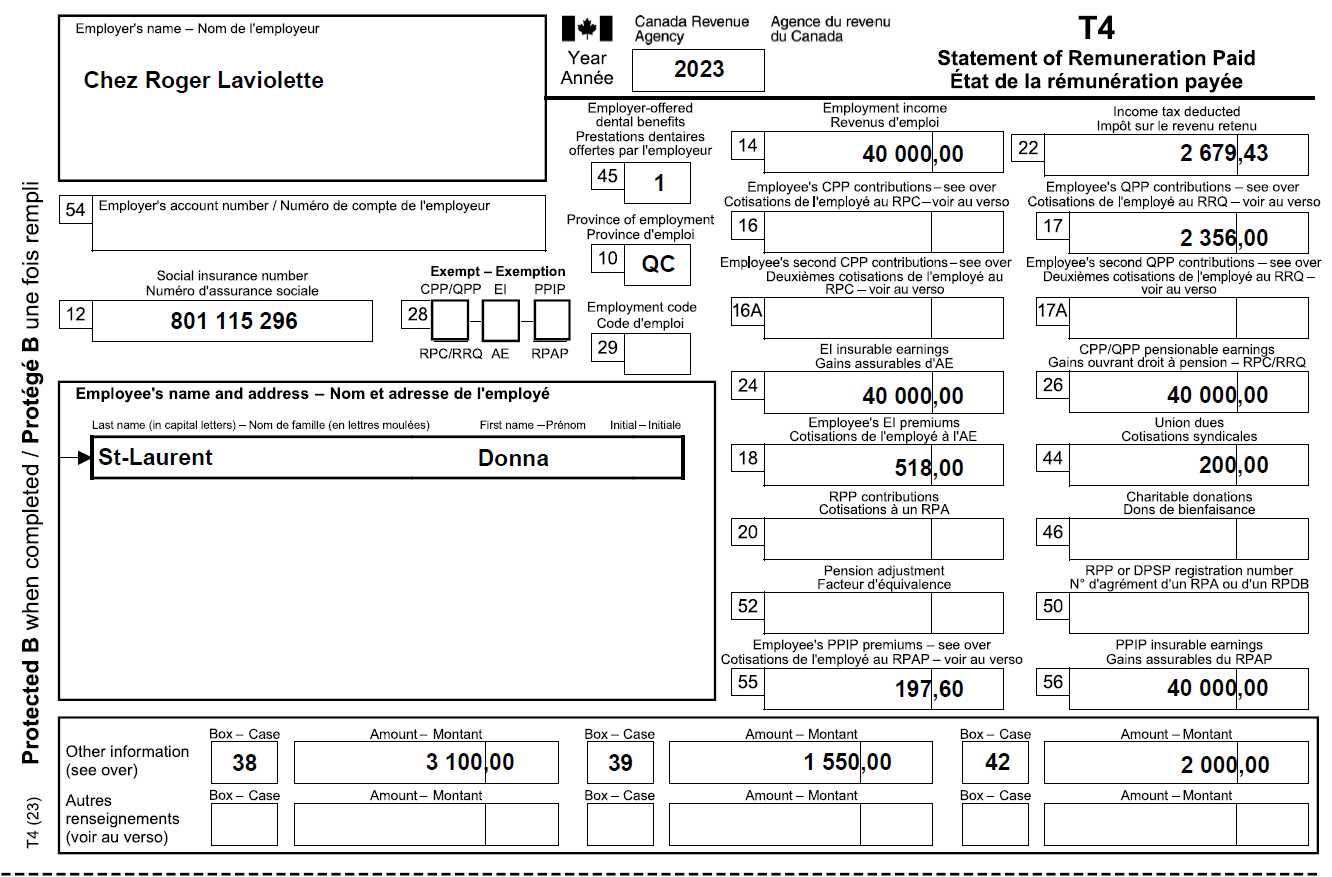
\includegraphics[width=.9\textwidth]{probleme/chapitre-3/T4.png}
	\caption{Problème, T4}
	\label{fig:chap3ProblemeT4}
\end{figure}
\begin{figure}
	\centering
	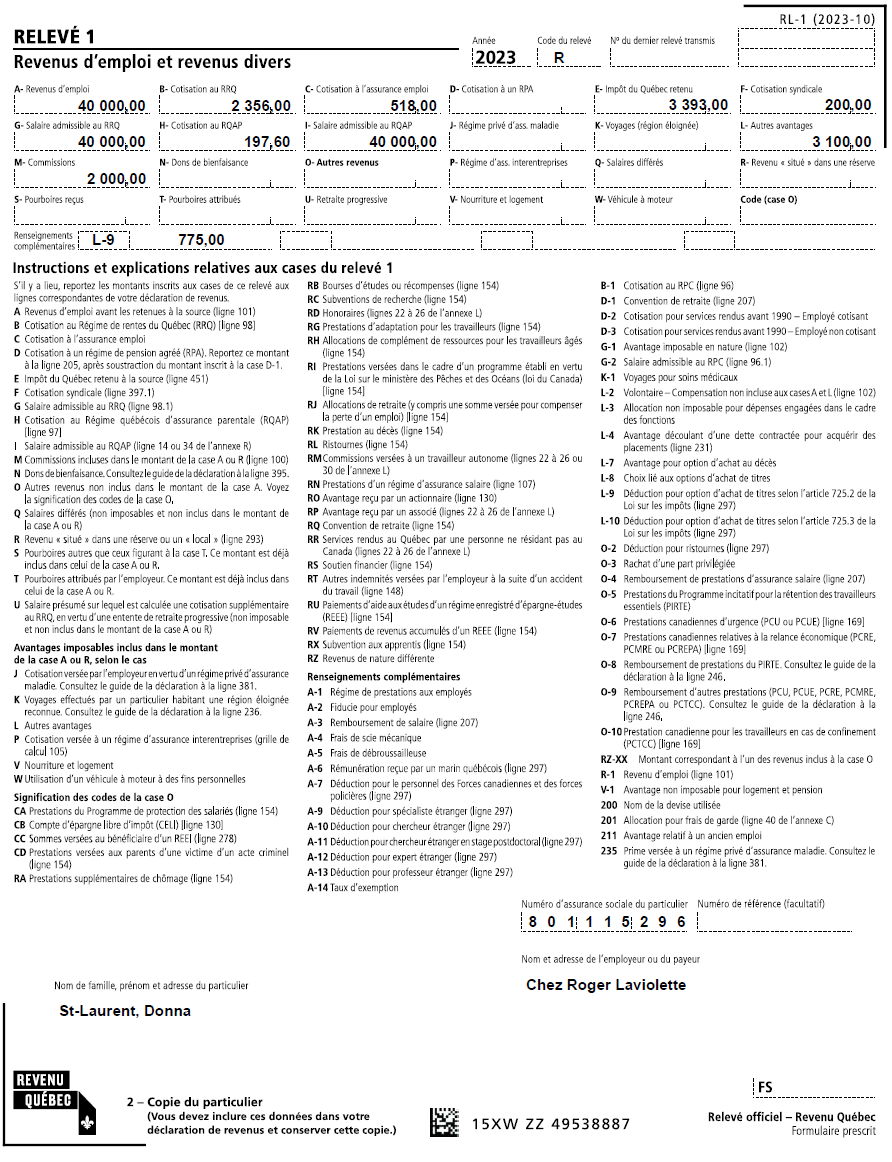
\includegraphics[width=.9\textwidth]{probleme/chapitre-3/RL1.png}
	\caption{Problème, RL-1}
	\label{fig:chap3ProblemeRL1}
\end{figure}



\subsection{Questions}
Complétez les étapes~2 à 4 de la \href{https://www.canada.ca/fr/agence-revenu/services/formulaires-publications/trousses-impot-toutes-annees-imposition/trousse-generale-impot-prestations/quebec/5005-r.html}{5005-R F} et pages~2 et 3 jusqu'à la ligne~299 de la \href{https://www.revenuquebec.ca/documents/fr/formulaires/tp/2023-12/TP-1.D%282023-12%29.pdf}{TP-1}.

\setcounter{question}{0}
\begin{question}
	À l'aide des renseignements figurant sur les feuillets d'impôt, calculez le trop-perçu au titre du RRQ, s'il y a lieu.
\end{question}
TP1, ligne 452 = Annexe 8, ligne 14 = 20,00

Gains ouvrant droit à pension RRQ (T4 case 26) = \numprint{40000,00} ou RL-1 case G qui a priorité

Cotisations de l’employé au RRQ (T4 case 17) = \numprint{2356,00}

Cotisations requises = (\numprint{40000,00} - \numprint{3500,00}) $\times$ 6,4 \% = \numprint{2336,00}, code 01 ligne 248 de la TP-1.

\begin{question}
	Effectuez les entrées appropriées aux lignes suivantes de la T1 et TP-1 de Donna.
	\begin{itemize}
		\item TP-1: lignes 98, 98.1 et 452 
		\item T1: lignes 30800 et 22215
	\end{itemize}
\end{question}
\begin{itemize}
	\item TP-1
	\begin{description}
		\item[Ligne 98] \numprint{2356,00} (Cotisation au RRQ, relevé 1, case B )
		\item[Ligne 98.1] \numprint{40000,00} (Salaire admissible au RRQ, relevé 1, case G)
		\item[Ligne 452] 20,00 (Cotisation payée en trop au RRQ)
	\end{description}
	\item T1
	\begin{description}
		\item[Ligne 30800] \numprint{1971,00} (Cotisations de base RRQ, Annexe 8, (\numprint{40000,00} -  \numprint{3500,00}) $\times$ 5,4~\%)
		\item[Ligne 22215] 365,00 (Déduction pour les cotisations bonifiées au RRQ, Annexe 8, (\numprint{40000,00} -  \numprint{3500,00}) $\times$ 1 \%)
	\end{description}
\end{itemize}

\begin{question}
	Calculez le paiement en trop à l'AE, le cas échéant, à l'aide de l'annexe 10.
\end{question}
Ligne 18 = \numprint{40000,00} (T4 case 24)

Ligne 20 = 508,00 = Ligne 22

Ligne 21 =  518,00 (T4 case 18)

Ligne 23 = 518,00 - 508,00 = 10,00

\begin{question}
	Quelles inscriptions devez-vous faire sur les déclarations fédérale et provinciale de Donna à l'égard de ses cotisations à l'AE?
\end{question}
31200 - Crédit d'impôt non remboursable : 40 000 (case 24) * 1,27 \% = 508,00

45000 - Paiement en trop d'AE : 10,00

Rien au provincial, c'est inclus dans le montant de base de la TP-1.

\begin{question}
	Calculez le paiement en trop au RQAP, le cas échéant.
\end{question}
Hors Québec, les prestations d'assurance parentale sont assumées par l'AE.

Au Québec, elles sont assumées par le RQAP.

Cotisation RQAP dû = \numprint{40000,00} (case I du RL-1) $\times$ 0,494 \% = 197,60

Cotisation RQAP payée = case H = 197,60 ; pas de paiement en trop

\begin{question}
	Effectuez les entrées appropriées aux lignes suivantes de la T1 et TP-1 de Donna.
	\begin{itemize}
		\item TP-1: lignes 97 et 457
		\item T1: ligne 31205
	\end{itemize}
\end{question}
\begin{itemize}
	\item TP-1
	\begin{description}
		\item[Ligne 97] 197,60 (Cotisation au RQAP, relevé 1, case H)
		\item[Ligne 457] 0,00 (Cotisation payée en trop au RQAP)
	\end{description}
	\item T1
	\begin{description}
		\item[Ligne 31205] 3197,60 (Cotisations au RPAP, T4, case 55)
	\end{description}
\end{itemize}

\begin{question}
	Ginette n'a eu aucun revenu durant l'année. Est-ce qu'elle doit produire une déclaration de revenus? Expliquez votre réponse.
\end{question}
Oui, T1, crédit pour la TPS (T1), crédit d'impôt pour solidarité + transfert crédits d'impôt non remboursable (TP-1)



\section{Autotest \no 1}
\setcounter{question}{0}
\begin{question}
	La grille d'imposition fédérale contient 5 tranches d'imposition. Combien y-a-t-il de tranches sur la grille d'imposition du Québec?
	\begin{enumerate}[label=\Alph*.]
		\item 3
		\item 4
		\item 5
		\item 6
	\end{enumerate}
\end{question}
4

\begin{question}
	Le contribuable a hérité de la somme de \numprint{2000}~\$ de ses parents. Son seul autre le revenu est de \numprint{40000}~\$ de revenu d'emploi. Quel taux d'imposition devra-t-il payer sur sa déclaration fédérale pour cet héritage ?
	\begin{enumerate}[label=\Alph*.]
		\item 0 \% - pas imposable
		\item 15 \%
		\item 20,5 \%
		\item 26 \%
	\end{enumerate}
\end{question}
0 \%

\begin{question}
	Que veut dire le \og revenu total \fg{}?
	\begin{enumerate}[label=\Alph*.]
		\item Tous les revenus moins (-)  toutes les déductions
		\item La somme de tous les revenus avant les déductions
		\item La somme de toutes les déductions avant les impôts
		\item Le revenu total est le revenu imposable moins (-) le revenu net
	\end{enumerate}
\end{question}
La somme de tous les revenus avant les déductions

\begin{question}
	Un contribuable a un revenu d'emploi de \numprint{21000}~\$. Quelle serait la déduction pour le travailleur à la ligne 201 de la TP-1?
	\begin{enumerate}[label=\Alph*.]
		\item 630~\$
		\item \numprint{1050}~\$
		\item \numprint{1260}~\$
		\item \numprint{1315}~\$
	\end{enumerate}
\end{question}
\numprint{1260}~\$

\begin{question}
	Un contribuable a payé une cotisation syndicale de 549~\$, indiquée à la case 44 de son T4. À quelle ligne de la T1, la cotisation syndicale doit être inscrite?
	\begin{enumerate}[label=\Alph*.]
		\item 23200
		\item 22200
		\item 22100
		\item 21200
	\end{enumerate}
\end{question}
21200
% Déductions et crédits d'emploi
\chapter{Montants personnels}
\section{Introduction et objectifs}
\subsection{Introduction}
Ce chapitre traite des montants personnels que le contribuable peut réclamer pour lui-même et les personnes qui sont à sa charge, y compris son époux ou conjoint de fait. Nous discuterons d'abord les crédits au fédéral, puis les crédits du Québec. 

Nous aborderons la réclamation des montants personnels lorsqu'il n'y a pas eu de changement dans la situation familiale au cours de l'année d'imposition.


\subsection{Objectifs}
\begin{itemize}[label=\twemoji{check mark button}]
	\item Expliquer ce que signifie une \og personne à charge \fg{};
	\item Déterminer quels sont les montants personnels qu'un contribuable peut demander pour lui-même, au fédéral et au Québec, et les réclamer sur les déclarations T1 et TP-1;
	\item Au fédéral, appliquer les règles régissant les demandes des montants suivants:
	\item Montant pour époux ou conjoint de fait;
	\begin{itemize}
		\item Montant canadien pour aidants naturels, pour époux ou conjoint de fait, ou pour une personne à charge admissible âgée de 18~ans ou plus;
		\item Montant pour une personne à charge admissible;
		\item Montant canadien pour aidants naturels pour autres personnes à charge âgées de 18~ans ou plus ayant une déficience;
		\item Montant canadien pour aidants naturels pour enfants âgés de moins de 18~ans ayant une déficience.
	\end{itemize}
	\item Au fédéral, expliquer en quoi consiste le crédit pour la TPS et comment en faire la demande et établir le montant;
	\item Au fédéral, expliquer en quoi consiste l'Allocation canadienne pour enfants (ACE) et la Prestation pour enfants handicapés (PEH), déterminer qui y est admissible et en faire la demande;
	\item Expliquer le crédit d'impôt pour solidarité accordé par le Québec
	\item Au Québec, expliquer en quoi consiste le paiement pour l'allocation famille, déterminer qui y est admissible et en faire la demande;
	\item Au Québec, appliquer les règles régissant les montants suivants:
	\begin{itemize}
		\item Le montant pour une personne vivant seule;
		\item Le montant pour enfant mineur aux études postsecondaires;
		\item Le montant transféré par un enfant majeur aux études postsecondaires;
		\item Le montant pour autres personnes à charge.
	\end{itemize}
\end{itemize}


\subsection{Sujets du chapitre}
\begin{itemize}
	\item Montants personnel au fédéral
	\item TPS et crédit de solidarité
	\item Montants personnels au Québec
	\item Programme allocation pour enfants
	\item Personnes à charge
\end{itemize}



\section{Crédits d'impôt non remboursables pour la famille}
\begin{intro}
	Dans le chapitre précédent, nous avions abordé les crédits d'impôt reliés à l'emploi. Maintenant c'est au tour des crédits d'impôt personnels. 
\end{intro}
Les crédits d'impôt non remboursables ont pour but de dédommager le contribuable pour les frais engagés afin de subvenir à ses besoins essentiels et à ceux des personnes dont il a la charge.



\section{Personnes à charge}
\begin{intro}
	Prendre soin d'une personne à charge amène son lot de responsabilités. Pour un support financier, vous pouvez compter sur l'aide gouvernementale pour vous accorder des crédits d'impôt.
	
	Plusieurs crédits d'impôt sont disponibles en fonction de la structure et de la situation de votre famille.
\end{intro}

\index{Personne à charge} 
Une \og personne à charge \fg{} est une personne qui compte sur le contribuable pour subvenir à ses besoins.

Aux fins de l'impôt, une personne à charge doit habituellement être liée au contribuable par les liens du sang, du mariage ou de l'adoption. 

Selon le montant personnel demandé, la personne à charge peut être l'une des personnes suivantes:
\begin{itemize}
	\item L'époux ou le conjoint de fait du contribuable;
	\item L'enfant ou le petit-enfant du contribuable ou de son époux ou conjoint de fait;
	\item La mère, le père, la grand-mère, le grand-père, la sœur, le frère du contribuable ou de son époux ou conjoint de fait; ou
	\item La tante, l'oncle, la nièce ou le neveu du contribuable ou de son époux ou conjoint de fait.
\end{itemize}

\begin{note}
	Dans de rares cas, l'interprétation de la notion de personne à charge peut différer entre l'ARC et RQ. 
	
	En cas de divergence d'opinions, il existe des moyens légaux de contestation.
\end{note}


\subsection{Subvenir aux besoins de la personne à charge}
Pour réclamer un montant à l'égard de la personne à charge, le contribuable doit avoir subvenu à ses besoins à un moment quelconque durant l'année d'imposition. 

Subvenir aux besoins signifie pourvoir à l'éducation, à la nourriture, à l'habillement, au logement, aux soins médicaux et aux autres besoins de la personne à charge.


\subsection{Revenu net de la personne à charge}
Pour la plupart des montants personnels (sauf une exception), le montant qui peut être réclamé par le contribuable à l'égard d'une personne à charge est réduit par le revenu net de cette dernière.

Dans la majorité des cas, lors du calcul d'un montant personnel, il faut tenir compte du revenu net de la personne à charge pour toute l'année, même si l'entretien n'a eu lieu qu'à un moment de l'année. 

La seule exception à cette règle est le montant pour époux ou conjoint de fait qui est réclamé dans l'année de séparation.

L'utilisation du revenu net dans le calcul d'un montant personnel se fait seulement après avoir déterminé qu'il s'agit effectivement d'une personne à charge.


\subsection{Définition des termes \og enfant \fg{} et \og parent \fg{}}
Les termes \og enfant \fg{} et \og parent \fg{} sont souvent utilisés pour désigner une personne à charge. La Loi de l'impôt sur le revenu définit \og enfant \fg{} de façon très élargie. La définition élargie du terme \og enfant \fg{} inclut:
\index{Enfant}
\begin{itemize}
	\item Un enfant naturel ou adoptif du contribuable. Un nouveau-né est considéré comme une personne à charge d'un particulier. Aucun montant ne peut être réclamé dans le cas d'un fœtus ou d'un enfant mort-né;
	\item Un enfant de l'époux ou conjoint de fait du contribuable;
	\item Une personne à charge qui n'est ni l'enfant naturel ni l'enfant adoptif du contribuable, mais qui est à la charge et sous le contrôle de ce dernier ou était sous sa garde et sous son contrôle avant qu'elle atteigne 19~ans. Ceci ne comprend pas un enfant en foyer nourricier pour lequel le contribuable reçoit des allocations spéciales d'une agence responsable de la garde d'enfants.
\end{itemize}

\index{Parent}
La définition élargie du terme \og parent \fg{} comprend toute personne reliée, soit le père, la mère, un fils, une fille, un frère, une sœur, un enfant adoptif, un petit-fils ou une petite-fille, un arrière-petit-fils ou une arrière-petite-fille, un grand-père ou une grand-mère. Elle couvre le même type de parenté \og non officielle \fg{} qui satisfait aux conditions d'admissibilité. La définition de parent ne comprend pas les oncles, les tantes, les neveux, ni les nièces, sauf si ces derniers entrent dans la définition élargie du mot \og enfant \fg{}, comme discuté précédemment.



\section{Montants personnels – Fédéral}
\begin{intro}
	Les montants personnels sont des crédits d'impôt non remboursables que le contribuable peut réclamer pour lui-même et pour les personnes qui sont à sa charge. L'objectif de ces crédits d'impôt est de compenser les frais de subsistance de base engagés par le contribuable pour lui-même et pour les personnes à sa charge.
\end{intro}

Dans ce chapitre, nous discuterons des six montants personnels fédéraux suivants:

\begin{enumerate}
	\item Le montant personnel de base (réclamé à la ligne~30000);
	\item Le montant pour époux ou conjoint de fait (réclamé à la ligne~30300);
	\item Le montant pour une personne à charge admissible (réclamé à la ligne~30400);
	\item Le montant canadien pour aidant naturel pour époux ou conjoint de fait, ou pour une personne à charge admissible âgée de 18~ans ou plus (réclamé à la ligne~30425);
	\item Le montant canadien pour aidant naturel pour autres personnes à charge âgées de 18~ans ou plus ayant une déficience (réclamé à la ligne~30450);
	\item Le montant canadien pour aidant naturel pour enfants âgés de moins de 18~ans ayant une déficience (réclamé à la ligne~30500).
\end{enumerate}

Chaque année, les montants personnels sont indexés, de même que le seuil du revenu servant à les établir. Cette indexation s'effectue en fonction de l'indice moyen des prix à la consommation au Canada au cours d'une période de douze mois. Pour 2023, le facteur d'indexation fédéral était de 6,3~\%.



\section{Exercice 1}
\setcounter{question}{0}
\begin{question}
	Qu'est-ce qu'une personne à charge aux fins de l'impôt?
\end{question}
Aux fins de l'impôt, une \og personne à charge \fg{} est une personne qui est liée au contribuable par les liens du sang, de l'adoption ou du mariage, et dont elle dépend pour ses besoins essentiels.

\begin{question}
	Pour réclamer un montant pour une personne à charge, est-ce que le contribuable doit subvenir aux besoins de cette personne pendant toute l'année?
\end{question}
Non.

Il ne suffit qu'un moment dans l'année pour que les besoins de cette personne à charge soient pourvus pour que le contribuable puisse réclamer le crédit d'impôt. Il n'est pas essentiel que ce soit pour toute l'année.

\begin{question}
	Nommez cinq montants personnels qui peuvent être réclamés sur la déclaration T1 et indiquez à quelle ligne ils peuvent l'être. Utilisez l'étape 5, partie B de la T1 pour vous aider.
\end{question}
\begin{enumerate}
	\item Le montant personnel de base, à la ligne~30000; 
	\item Le montant pour époux ou conjoint de fait, à la ligne~30300; 
	\item Le montant pour une personne à charge admissible, à la ligne~30400;
	\item Le montant canadien pour aidants naturels pour époux ou conjoint de fait, ou pour une personne à charge admissible âgée de 18~ans ou plus, à la ligne~30425;
	\item Le montant canadien pour aidants naturels pour autres personnes à charge âgées de 18~ans ou plus ayant une déficience, à la ligne~30450;
	\item Le montant canadien pour aidants naturels pour enfants âgés de moins de 18~ans ayant une déficience, à la ligne~30500.
\end{enumerate}



\section{Montant personnel de base et Montant pour époux ou conjoint de fait}
\begin{intro}
	Chaque contribuable peut demander un montant personnel de base. Si le contribuable a un époux ou un conjoint de fait dont le revenu net est inférieur au montant personnel de base, il peut alors demander un montant pour son époux ou conjoint de fait. 
	
	Si la personne à charge pour laquelle un montant personnel est demandé souffre d'une déficience mentale ou physique, le \acrfull{ccan} est un crédit d'impôt non remboursable qui peut être disponible.
\end{intro}


\subsection{Montant personnel de base (ligne~30000)}
Pour 2023, le montant personnel de base est calculé en fonction du revenu net du contribuable comme suit:
\begin{itemize}
	\item Si le revenu net du contribuable est inférieur ou égal à \numprint{165430}~\$, le montant est de \numprint{15000}~\$;
	\item Si le revenu net du contribuable est supérieur ou égal à \numprint{235675}~\$, le montant est de \numprint{13520}~\$;
	\item Si le revenu net du contribuable se situe entre \numprint{165430}~\$ et \numprint{235675}~\$, le montant de \numprint{15000}~\$ est réduit proportionnellement. La grille de calcul de la ligne~30000 doit être utilisée pour calculer le montant de base réel.
\end{itemize}

\begin{note}
	Pour les besoins de compréhension des sujets suivants, aucune discussion sur un changement d'état civil n'aura lieu. Ce sujet sera discuté dans un autre chapitre.
\end{note}


\subsection{Montant canadien pour aidant naturel}
Dans le cadre de la discussion des montants personnels suivants, le montant demandé par le contribuable peut être majoré de \numprint{2499}~\$ (en 2023), si la personne à charge pour laquelle le montant est demandé a une déficience mentale ou physique. 

Ce montant fixe est le Montant canadien pour aidant naturel. La déficience doit être attestée par écrit par un professionnel de la santé. 

Ce montant est soit demandé en plus du montant personnel, soit déjà inclus dans le montant du crédit. 

Les crédits suivants exigent que le contribuable demande le Montant canadien pour aidants naturels comme un ajout.
\begin{itemize}
	\item Le montant pour époux ou conjoint de fait (ligne~30300);
	\item Le montant pour une personne à charge admissible (ligne~30400).
\end{itemize}

Les crédits suivants, qui sont des crédits autonomes destinés spécifiquement aux personnes à charge souffrant d'une infirmité, intègrent déjà le montant canadien pour aidants naturels:
\begin{itemize}
	\item Le Montant canadien pour aidant naturel pour l'époux ou le conjoint de fait, ou pour votre personne à charge admissible âgée de 18~ans ou plus (ligne~30425);
	\item Le Montant canadien pour aidant naturel pour les autres personnes à charge âgées de 18~ans ou plus ayant une déficience (ligne~30450);
	\item Le Montant canadien pour aidant naturel pour les enfants infirmes de moins de 18~ans (ligne~30500).
\end{itemize}

À l'exception du Montant canadien pour aidant naturel pour les enfants déficients de moins de 18~ans (ligne~30500), nous verrons que l'annexe~5 est utilisée pour calculer le montant à demander pour chaque crédit.

Si le contribuable a plus d'une personne à charge souffrant d'une déficience mentale ou physique, le montant supplémentaire \numprint{2499}~\$ peut être demandé pour chaque personne à charge. 

Toutefois, si plus d'un des montants ci-dessus peut être demandé pour la même personne à charge, le Montant canadien pour aidant naturel ne peut être demandé qu'une seule fois pour chaque personne à charge.

\subsubsection{Degré de déficience mentale ou physique}
Le degré de déficience mentale ou physique nécessaire pour le montant canadien pour aidant naturel diffère pour les enfants de moins de 18~ans et pour les personnes à charge de 18~ans ou plus:
\begin{itemize}
	\item Dans le cas d'un enfant de moins de 18~ans qui souffre d'une infirmité mentale ou physique, cette déficience doit être prolongée et être d'une période indéterminée. L'enfant doit dépendre plus des autres pour ses besoins et soins personnels, comparativement aux enfants du même âge;
	\item Dans le cas d'une personne à charge de 18~ans ou plus, cette personne doit dépendre du contribuable en raison d'une déficience mentale ou physique.
\end{itemize}

\subsubsection{Signification de déficience}
La \textbf{Loi de l'impôt sur le revenu} ne donne pas de définition du mot \og déficience \fg{}. Par conséquent, on doit lui donner sa signification générale.  L'ARC affirme que dans le cas d'une personne qui souffre d'une déficience mentale ou physique, cette déficience doit l'empêcher d'être entièrement autonome. La dépendance de la personne à charge doit provenir uniquement du fait qu'elle souffre de cette déficience. À cet effet, une incapacité temporaire n'est donc pas considérée comme une déficience physique ou mentale.

Si une personne à charge a droit au montant pour personnes handicapées et que le formulaire T2201, Crédit d'impôt pour personnes handicapées, figure dans les dossiers de l'ARC, il faut donc supposer qu'elle aura également droit au montant canadien pour aidants naturels. 

Lorsque la déficience de la personne à charge n'est pas assez grave pour donner droit au crédit d'impôt pour personnes handicapées, mais qu'elle pourrait donner droit au montant canadien pour aidants naturels, le contribuable doit avoir une déclaration signée d'un médecin attestant de la nature et de la durée de la déficience. Il n'est pas nécessaire de joindre ce document à la déclaration T1. Toutefois, le contribuable doit être en mesure de le présenter sur demande.


\subsection{Montant pour époux ou conjoint de fait (ligne~30300)}
Les contribuables peuvent demander un montant pour leur époux ou conjoint de fait si, à un moment donné de l'année, ils ont subvenu aux besoins de leur époux ou conjoint de fait.

Seul l'un des époux ou conjoints de fait peut demander ce montant pour l'autre.

\subsubsection{Définition de \og époux \fg{} et \og conjoint de fait \fg{}}
\index{Époux}
\index{Conjoint de fait}
Pour l'ARC, un \og époux \fg{} est la personne avec laquelle le contribuable est légalement marié.

Un \og conjoint de fait \fg{} désigne une personne, de même sexe ou de sexe opposé, qui n'est pas l'époux du contribuable, qui vit avec lui dans une relation conjugale et qui remplit l'une des conditions suivantes:
\begin{itemize}
	\item Cette personne vit avec le contribuable dans cette relation depuis au moins 12 mois consécutifs. La période de 12 mois comprend toute période de séparation de moins de 90~jours;
	\item Cette personne est le parent de l'enfant du contribuable par sa naissance ou son adoption; ou
	\item Cette personne a la garde, la surveillance et la charge entière de l'enfant du contribuable (ou en avait la garde et la surveillance juste avant que l'enfant atteigne l'âge de 19~ans).
\end{itemize}

\begin{rappel}
	Le revenu net de l'époux ou conjoint de fait est le montant que le contribuable doit inscrire dans la partie \og Renseignements sur votre époux ou conjoint de fait \fg{} de la page 1 de la T1.
\end{rappel}

Le montant pour époux ou conjoint de fait est calculé comme suit sur la grille de calcul de la ligne~30300 de l'annexe~5:
\begin{itemize}
	\item Le montant personnel de base du contribuable; plus
	\item Le Montant canadien pour aidant naturel (si admissible); moins
	\item Le revenu net de l'époux ou conjoint de fait.
\end{itemize}


\section{Montants pour personne à charge admissible et pour personne à charge ayant une déficience}
\begin{intro}
	La demande de montants personnels pour les personnes à charge autres que le conjoint ou le conjoint de fait requiert davantage de conditions à remplir.
\end{intro}


\subsection{Montant pour une personne à charge admissible (ligne~30400)}
Le montant pour une personne à charge admissible a pour but d'alléger le fardeau des contribuables célibataires, divorcés, séparés ou veufs qui ont au moins une personne à leur charge. 

Toutefois, si le contribuable a plus d'une personne à charge admissible, cette demande ne peut être faite qu'à l'égard d'une seule de ces personnes à charge.

Pour réclamer le montant pour une personne à charge admissible, plusieurs caractéristiques doivent être prises en compte:
\begin{itemize}
	\item État civil du contribuable;
	\item Niveau de soutien fourni;
	\item Lien de la personne à charge avec le contribuable;
	\item Résidence de la personne à charge;
	\item Âge de la personne à charge;
	\item Invalidité;
	\item Si la personne à charge a été déclarée comme personne à charge par un autre contribuable.
\end{itemize}

\begin{note}
	Ce sujet particulier peut être difficile à comprendre.
	
	Les conditions d'admissibilité au montant pour une personne à charge admissible sont présentées dans la figure \ref{fig:MontantPourUnePersonneAChargeAdmissible}. Utilisez ce tableau pour identifier les critères d'admissibilité du montant pour personne à charge admissible.
\end{note}

\begin{figure}
	\centering
	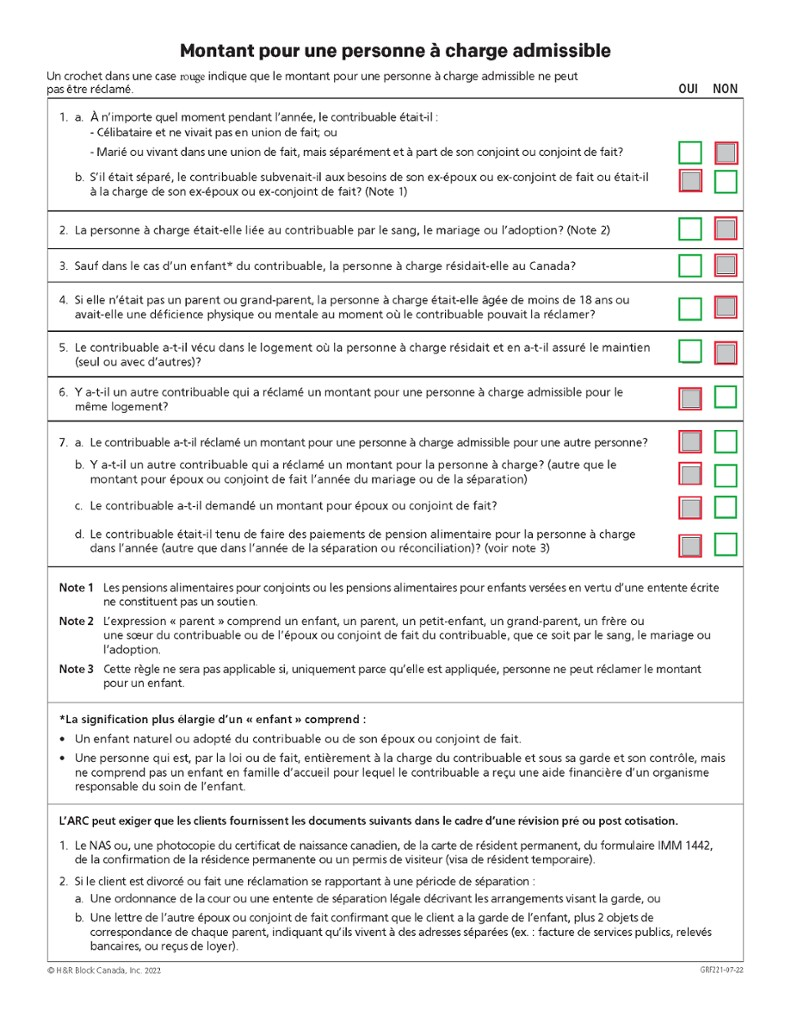
\includegraphics[width=.95\textwidth]{Montant-pour-une-personne-a-charge-admissible.jpg}
	\caption{Montant pour une personne à charge admissible}
	\label{fig:MontantPourUnePersonneAChargeAdmissible}
\end{figure}

\subsubsection{État civil}
Pour avoir droit à ce montant, le contribuable ne devait pas avoir d'époux ou de conjoint de fait lorsqu'il subvenait aux besoins de la personne à charge.

\subsubsection{Garde partagée}
Dans le cas d'une garde partagée, le contribuable et l'autre parent de l'enfant doivent décider ensemble qui demandera le montant pour la personne à charge admissible concernant l'enfant, sinon aucun d'entre eux n'y aura droit.

Le montant pour une personne à charge admissible ne peut pas être partagé, d'où l'importance de prendre une décision concernant le parent qui réclamera ce crédit.

Les parents séparés qui font partie d'un nouveau couple ne peuvent pas demander le montant pour une personne à charge admissible.

\subsubsection{Soutien}
Pour réclamer le montant pour personne à charge admissible, le contribuable doit pourvoir à l'éducation, la nourriture, l'habillement, au logement et à tous les autres besoins de la personne à charge admissible.

\subsubsection{Relations parentales}
\begin{rappel}
	Une personne à charge admissible n'est pas nécessairement un enfant.
\end{rappel}

Le montant pour personne à charge admissible peut être réclamé seulement à l'égard d'une des personnes suivantes:

L'enfant ou le parent du contribuable ou de son époux ou conjoint de fait;
\begin{itemize}
	\item Un descendant ou un ascendant en ligne directe du contribuable ou de son époux ou conjoint de fait (petit-enfant, arrière-petit-enfant, grand-parent ou arrière-grand-parent);
	\item L'époux ou conjoint de fait d'un descendant ou un ascendant en ligne directe du contribuable ou de son époux ou conjoint de fait;
	\item Le frère ou la sœur du contribuable ou ceux de son époux ou conjoint de fait;
	\item L'époux ou le conjoint de fait du frère ou de la sœur du contribuable, l'époux ou le conjoint de fait du frère ou de la sœur de son époux ou conjoint de fait.
\end{itemize}

Même si les oncles, les tantes, les neveux et les nièces ne font pas partie de la liste ci-dessus, le contribuable peut réclamer le montant pour une personne à charge admissible pour ces personnes, si elles répondent à la définition élargie du terme \og enfant \fg{} ou du terme \og parent \fg{}, comme nous l'avons discuté précédemment.

\subsubsection{Résidence}
La personne à charge doit résider au Canada, sauf si cette personne est l'enfant du contribuable et qu'elle a vécu avec ce dernier. Un enfant qui ne réside pas avec le contribuable en raison de ses études est considéré comme vivant normalement avec ce dernier.

Les visiteurs ne peuvent pas être réclamés.

\subsubsection{Âge}
Un contribuable peut réclamer un montant pour une personne à charge admissible si cette dernière respectait une des conditions ci-dessous:
\begin{itemize}
	\item Avait moins de 18~ans à un moment de l'année;
	\begin{itemize}
		\item Si, dans l'année d'imposition, la personne à charge a eu 18~ans le 2 janvier, elle est admissible même si elle avait moins de 18~ans pour une seule journée.
	\end{itemize}
	\item Avait 18~ans ou plus et avait une déficience mentale ou physique; ou
	\item Est un parent ou grand-parent.
\end{itemize}

Un contribuable célibataire dont le parent ou le grand-parent est à sa charge peut donc réclamer le montant pour une personne à charge admissible sans tenir compte de l'âge ni de la déficience. 

Par contre, un contribuable dont l'enfant, le petit-enfant, le frère ou la sœur est à sa charge ne peut pas réclamer le montant pour une personne à charge admissible à l'égard de cette personne, sauf si cette dernière est âgée de moins de 18~ans ou souffre d'une déficience mentale ou physique.

\paragraph{Illustration}
Jacques est célibataire. Il subvient aux soins et à l'éducation de son neveu Sébastien qui est âgé de 16~ans. Jacques peut réclamer le montant pour une personne à charge admissible à l'égard de Sébastien, parce que ce dernier est considéré être l'enfant de Jacques, selon la définition du terme \og enfant \fg{}.

Si Jacques a la garde et la surveillance de Sébastien jusqu'à ce que ce dernier atteigne 19~ans, Sébastien continuera d'être considéré comme l'enfant de Jacques, même s'il n'est plus sous sa garde et sa surveillance. S'il satisfait aux autres conditions, Jacques pourra continuer à réclamer ce montant pour Sébastien.

\subsubsection{Maintien du domicile}
Le contribuable doit avoir maintenu le logement dans lequel lui et la personne à charge résident. Le logement doit être un établissement domestique autonome au sens de la loi, c'est-à-dire une maison, un appartement ou un autre logement de ce genre où une personne mange et dort habituellement. Une chambre dans une maison de pension ou une chambre d'hôtel ne constitue pas un établissement domestique autonome.

Un contribuable peut réclamer un montant pour une personne à charge admissible à l'égard d'une personne qui ne vit pas avec lui à cause de ses études, à condition que cette personne revienne habiter avec lui quand elle n'est pas à l'école.

\subsubsection{Une seule demande par logement}
Si le contribuable a maintenu le logement avec quelqu'un d'autre, une seule personne dans la maisonnée peut faire la demande du montant pour une personne à charge admissible. Le montant ne peut pas être partagé.

\paragraph{Illustration}
Deux sœurs divorcées vivent dans le même logement. Elles ont un enfant chacune. Les enfants sont âgés de 15~ans. Il n'y a qu'une seule des deux sœurs qui peut réclamer le montant pour une personne à charge admissible à l'égard de son propre enfant. Le même montant ne peut être accordé deux fois dans la maisonnée.

Cependant, elles peuvent décider d'alterner annuellement la réclamation du montant pour personne à charge admissible.

\subsubsection{Autres particularités}
Lorsque l'on analyse la possibilité de réclamer le montant pour une personne à charge admissible, il faut également tenir compte des restrictions
suivantes:
\begin{itemize}
	\item Le contribuable ne peut pas réclamer le montant pour époux ou conjoint de fait et le montant pour une personne à charge admissible. Même si le couple a un enfant mineur, il ne peut pas réclamer le montant pour personne à charge admissible;
	\item Même si plusieurs personnes sont à sa charge, le contribuable ne peut réclamer qu'un seul montant pour une personne à charge admissible. Il doit donc choisir la personne qui lui permettra de faire la réclamation la plus avantageuse;
	\item Un contribuable ne peut pas réclamer le montant pour une personne à charge admissible à l'égard d'une personne qu'un autre contribuable réclame à titre de montant pour époux ou conjoint de fait, si cette personne a été mariée ou avait un conjoint de fait pendant toute l'année et qu'elle n'était pas séparée à cause de la rupture de son union;
	\item Un contribuable ne peut pas réclamer le montant pour une personne à charge admissible à l'égard d'un enfant pour lequel il est tenu de verser une pension alimentaire.
\end{itemize}

\subsubsection{Traitement fiscal}
La partie \og ligne~30400 \fg{} de l'annexe~5, présentée à l'illustration 4-5, permet de calculer le montant pour une personne à charge admissible. Le montant obtenu est reporté à la ligne~30400 de la T1. Procédez comme suit:

\begin{itemize}
	\item Inscrivez la date du changement de l'état civil s'il y a lieu.
	\item Entrez les informations de la personne à charge admissible. Si la personne à charge est mineure, il se peut qu'il n'y ait pas de NAS. Dans ce cas, laissez le champ libre. 
	\item La plupart du temps, l'adresse de la personne à charge est la même que celle du contribuable, puisque la personne à charge doit vivre avec le contribuable pendant la période pour laquelle il réclame le montant. Cependant, si la personne à charge a déménagé depuis, l'adresse sera différente.
	\item Répondez à la question si la personne à charge a une déficience.
	\item Calculez la réclamation, qui doit être égale au montant personnel de base du contribuable plus le montant canadien pour aidant naturel (si la réponse à la question sur la déficience est positive) moins le revenu net de la personne à charge.
	\begin{note}
		Si la personne à charge est un enfant infirme de moins de 18~ans, le Montant canadien pour aidant naturel ne doit pas être demandé à la ligne~30400. Il doit être demandé séparément à la ligne~30500. Nous discuterons cette réclamation plus loin dans ce chapitre.
	\end{note}
	\item Reportez le montant à la ligne~30400 de la T1.
\end{itemize}


\subsection{Montant canadien pour aidant naturel pour un époux ou conjoint de fait, ou pour une personne à charge admissible âgée de 18~ans ou plus (ligne~30425)}
Ce crédit supplémentaire ne peut être demandé que si le contribuable a demandé le montant pour époux ou conjoint de fait ou le montant pour une personne à charge admissible (pour une personne à charge âgée de 18~ans ou plus) \textbf{et} qui a une déficience physique ou mentale qui rend la personne admissible au Montant canadien pour aidant naturel. 

Ce crédit ne doit être demandé que si ces personnes ont un revenu net compris entre \numprint{8020}~\$ et \numprint{26782}~\$. 

Pour demander le crédit, le contribuable doit d'abord remplir soit la ligne~30300 de l'annexe~5, s'il demande le crédit pour un conjoint, soit la ligne~30400 de l'annexe~5, s'il demande le crédit pour une personne à charge admissible. Le Montant canadien pour aidant naturel doit être demandé avec chacun de ces montants.

\begin{rappel}
	N'oubliez pas qu'un contribuable ayant un époux ou un conjoint de fait pendant toute l'année ne peut pas présenter de demande pour une personne à charge admissible.
\end{rappel}

Le contribuable remplit ensuite l'annexe~5 ligne~30425 en soustrayant d'abord le revenu net de la personne à charge (ligne~23600 de sa déclaration) de \numprint{26782}~\$. La différence qui en résulte est plafonnée à\numprint{7999}~\$. Le contribuable soustrait ensuite du résultat le montant qu'il a demandé à la ligne~30300 ou à la ligne~30400 et demande le solde à la ligne~30425.

\subsubsection{Montant canadien pour aidant naturel pour autres personnes à charge âgées de 18~ans ou plus ayant une déficience (ligne~30450)}
Un contribuable peut réclamer le montant canadien pour aidant naturel pour autres personnes à charge âgées de 18~ans ou plus ayant une déficience pour chacune des personnes qui répond à toutes les conditions suivantes:
\begin{itemize}
	\item Cette personne est un de ses parents, grands-parents, frères, sœurs, oncles, tantes, neveux, nièces, y compris ceux de son époux ou conjoint de fait, selon la définition élargie d'un \og enfant \fg{} ou d'un \og parent \fg{};
	\item Elle est âgée de 18~ans ou plus à la fin de l'année (née en 2005 ou avant);
	\item Elle est à la charge du contribuable ou à charge partagée avec d'autres personnes;
	\item Elle a une déficience des fonctions mentales ou physiques;
	\item Elle a résidé au Canada à un moment de l'année.
\end{itemize}

\begin{note}
	Le contribuable ne peut pas demander ce montant pour une personne qui lui rendait visite seulement.
\end{note}

\index{Parent}
Le mot \og parent \fg{} désigne une personne dont le contribuable était entièrement à la charge et qui avait le contribuable sous sa garde et sa surveillance lorsque ce dernier avait moins de 19~ans. 

\index{Enfant}
Le mot \og enfant \fg{} désigne toute personne qui est devenue entièrement à la charge du contribuable, même si elle est plus âgée que lui.

\subsubsection{Autres particularités}
Les autres caractéristiques du Montant canadien pour aidant naturel pour autres personnes à charge âgées de 18~ans ou plus ayant une déficience sont les suivantes:
\begin{itemize}
	\item Le montant canadien pour aidant naturel pour autres personnes à charge âgées de 18~ans ou plus ayant une déficience peut être partagé avec une autre personne qui a subvenu aux besoins de la personne à charge. Par conséquent, deux contribuables peuvent faire une demande pour la même personne à charge. Il faut toutefois que le total des montants combinés ne dépasse pas le maximum admissible pour cette personne à charge.
	\item Si un contribuable réclame le \og montant pour une personne à charge admissible \fg{} (ligne~30400) à l'égard d'une personne à charge, il ne peut pas réclamer un montant canadien pour aidants naturels pour autres personnes à charge âgées de 18~ans ou plus ayant une déficience (ligne~30450) pour cette même personne à charge.
\end{itemize}

Il y a des situations où un contribuable a la possibilité de réclamer plusieurs montants et qu'il doive faire un choix. Il doit alors étudier les faits afin de déterminer quelle combinaison est la plus avantageuse.

\paragraph{Illustration}
Bernard vit seul avec ses deux filles: Sylvie, âgée de 19~ans, et Martine, âgée de 17~ans, qui sont entièrement à sa charge. Sylvie a une déficience physique, justifiée par une lettre d'un médecin. Les deux sœurs n'ont eu aucun revenu.

Quel montant Bernard peut-il réclamer pour ses filles? Quelles sont ses options?

Si Bernard choisit de demander le montant pour une personne à charge admissible pour Martine parce qu'elle a moins de 18~ans, il ne peut pas demander le montant pour une personne à charge admissible pour Sylvie (N.B. Elle a plus de 18~ans, mais elle est handicapée).
Si Bernard choisit de demander le montant pour une personne à charge admissible pour Sylvie, il ne peut pas demander le montant pour une personne à charge admissible pour Martine.
Si Bernard choisit de demander le montant canadien pour aidant naturel pour d'autres personnes à charge âgées de 18~ans ou plus ayant une déficience pour Sylvie, il ne peut pas demander le montant pour la personne à charge admissible pour Sylvie. Cependant, il peut demander le montant pour la personne à charge admissible pour Martine.

Pour l'aider à prendre sa décision, Bernard doit calculer le montant qu'il peut réclamer pour chaque option.

En supposant que le montant personnel de base de Bernard est de \numprint{15000}~\$, les résultats pour chaque option ci-dessus sont les suivants:

\begin{enumerate}
	\item \numprint{14398}~\$;
	\item \numprint{16748}~\$;
	\item \numprint{7525}~\$ + \numprint{14398}~\$ =  \numprint{21923}~\$
\end{enumerate}

Après réflexion, c'est plus avantageux pour Bernard de choisir l'option 3 et de réclamer le montant pour personne à charge admissible pour Martine et le montant canadien pour aidant naturel pour autres personnes à charge âgées de 18~ans ou plus ayant une déficience pour Sylvie.

\subsubsection{Montant canadien pour aidant naturel pour enfants âgés de moins de 18~ans ayant une déficience (ligne~30500)}
Le contribuable peut demander un montant canadien pour aidant naturel de
\numprint{2499}~\$ pour chacun de ses enfants ou ceux de son époux ou conjoint de fait qui remplit toutes les conditions suivantes:
\begin{itemize}
	\item L'enfant a moins de 18~ans à la fin de l'année;
	\item L'enfant a résidé habituellement avec ses \textbf{deux} parents tout au long de l'année;
	\item Il a une déficience des fonctions mentales ou physiques
\end{itemize}.

Il n'y a pas de limite du revenu net pour le contribuable ou les enfants.
Rappel.

\begin{rappel}
	Pour les enfants de moins de 18~ans, la déficience doit être prolongée et indéfinie. Cela signifie qu'ils ont besoin de beaucoup plus d'assistance pour leurs besoins personnels et leurs soins que les enfants du même âge.
\end{rappel}

Le contribuable doit inscrire le nombre d'enfants de moins de 18~ans admissibles au montant canadien pour aidants naturels à la ligne~30499 de la T1 et inscrire la réclamation totale à la ligne~30500.

\subsubsection{Autres particularités}
Les autres caractéristiques du Montant canadien pour aidant naturel pour les enfants handicapés de moins de 18~ans sont les suivantes:
\begin{itemize}
	\item Le contribuable peut demander le montant même s'il ne peut pas demander le montant pour une personne à charge admissible, parce que le revenu net de l'enfant est élevé ou parce qu'il demande déjà le montant pour une personne à charge admissible pour un autre enfant;
	\item Un contribuable peut demander le montant canadien pour aidant naturel même s'il habite un logement avec une autre personne;
	\item Un contribuable peut transférer à son époux ou conjoint de fait une partie ou la totalité du montant pour enfants dont il n'a pas besoin pour réduire ses impôts à payer à zéro. À l'inverse, il peut demander une partie ou la totalité du montant que son époux ou conjoint de fait n'utilise pas. La partie inutilisée qui peut être transférée est calculée sur l'annexe~2.
\end{itemize}


\subsection{annexe~2}
L'annexe~2 est utilisée pour transférer certains crédits non remboursables entre époux ou conjoints de fait si tout ou partie de ces crédits ne sont pas nécessaires pour réduire à zéro l'impôt à payer par le contribuable.

Le premier cas d'utilisation de l'annexe~2 concerne le Montant canadien pour les aidants naturels d'enfants handicapés de moins de 18~ans.

Les autres cas sont: 
\begin{itemize}
	\item Montant pour personne handicapée: discuté au chapitre 9;
	\item Montant en raison de l'âge: discuté au chapitre 10;
	\item Montant pour revenu de pension: discuté au chapitre 10;
	\item Montant pour frais de scolarité: discuté au chapitre 12.
\end{itemize}

\begin{note}
	Au Québec, le montant pour un aidant naturel est un crédit d'impôt remboursable et est étudié dans un autre chapitre.
\end{note}

\cat\href{https://www.canada.ca/fr/agence-revenu/services/impot/particuliers/sujets/tout-votre-declaration-revenus/declaration-revenus/remplir-declaration-revenus/deductions-credits-depenses/montant-aidants-naturels.html}{Crédit canadien pour aidant naturel}



\section{Exercice 2}
\setcounter{question}{0}
\begin{question}
	Bogdan et Alena ont deux enfants: Jaroslav, né le 16 août 2010 (13~ans) et Danica, née le 2 février 2013 (10~ans). Le revenu net de Bogdan est de \numprint{28500}~\$ et celui d'Alena de \numprint{9598}~\$. Alena et Danica souffrent toutes deux d'un handicap physique attesté par leur médecin.
	
	Quels montants personnels Bogdan peut-il demander? Remplissez les lignes appropriées de l'\href{https://www.canada.ca/fr/agence-revenu/services/formulaires-publications/trousses-impot-toutes-annees-imposition/trousse-generale-impot-prestations/5000-s5.html}{annexe~5} et les lignes~30000 à 30500 de l'étape 5 de la partie B de la déclaration \href{https://www.canada.ca/fr/agence-revenu/services/formulaires-publications/trousses-impot-toutes-annees-imposition/trousse-generale-impot-prestations/quebec/5005-r.html}{T1}.
\end{question}
annexe~5, ligne~30300: figure \ref{fig:chap4Exercice2Q130300}
\begin{figure}
	\centering
	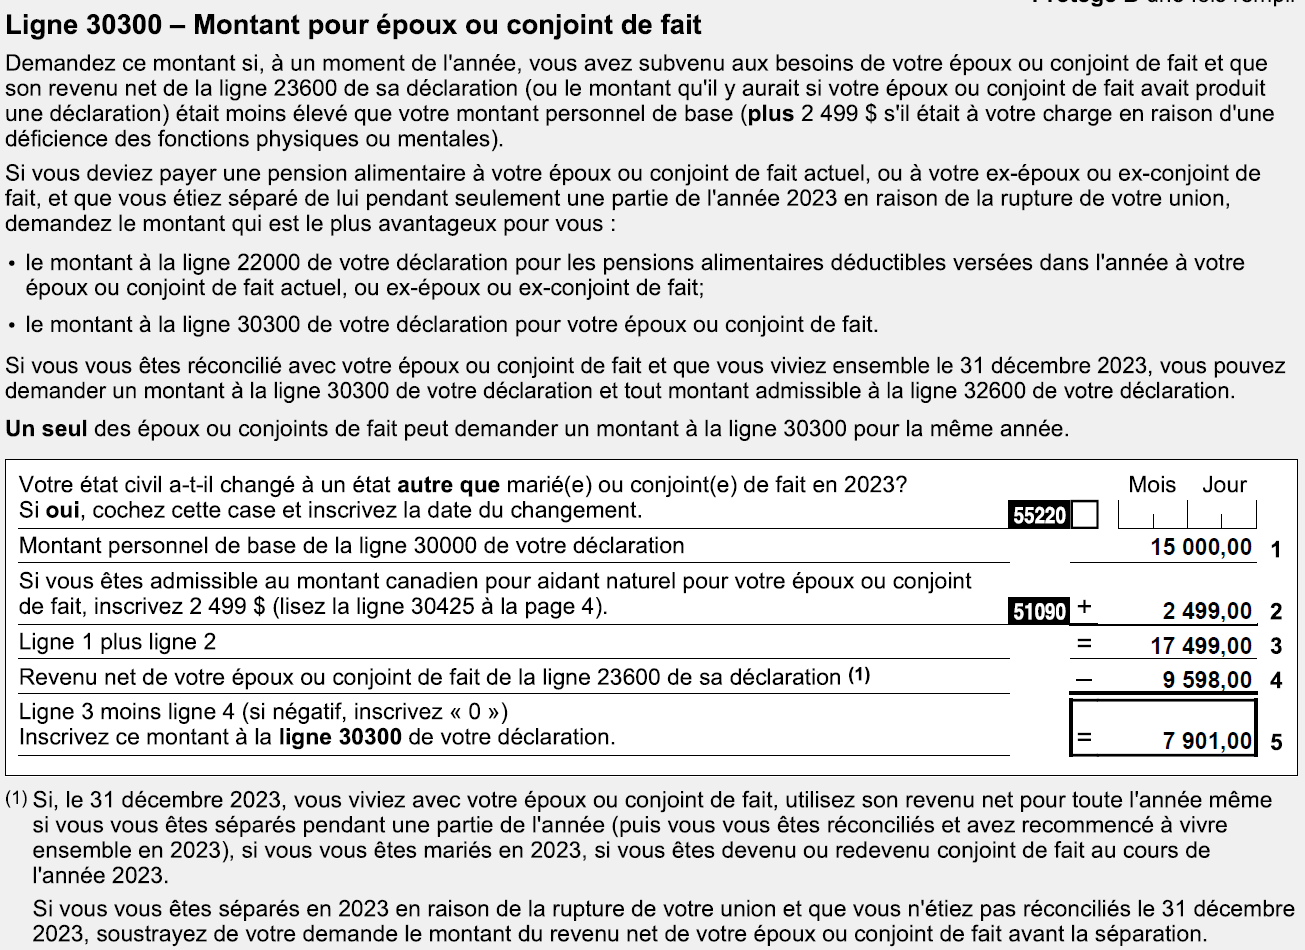
\includegraphics[width=.9\textwidth]{exercice/4-2/Q1/30300.png}
	\caption[]{Exercice 2, annexe~5, ligne~30300}
	\label{fig:chap4Exercice2Q130300}
\end{figure}

annexe~5, ligne~30425: figure \ref{fig:chap4Exercice2Q130425}
\begin{figure}
	\centering
	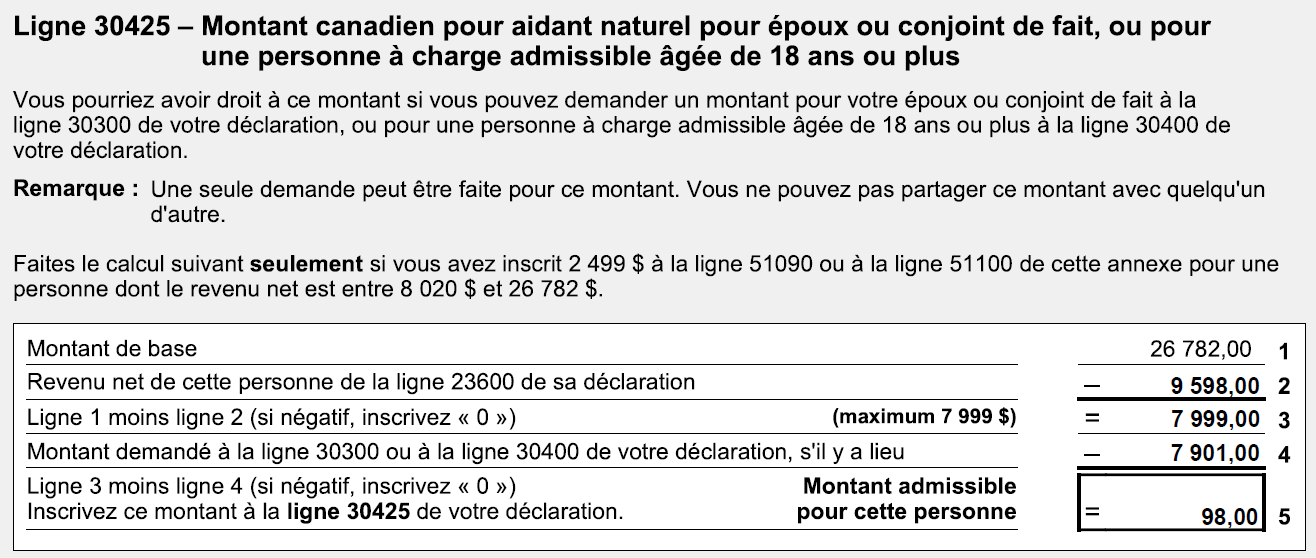
\includegraphics[width=.9\textwidth]{exercice/4-2/Q1/30425.png}
	\caption[]{Exercice 2, annexe~5, ligne~30425}
	\label{fig:chap4Exercice2Q130425}
\end{figure}

Partie B de l'étape 5 de la 5005-R F, page 5: figure \ref{fig:chap4Exercice2Q1T1B}:
\begin{description}
	\item[Ligne~30000] Montant personnel de base de Bogdan.
	\item[Ligne~30300] Montant pour époux ou conjoint de fait, y compris le montant canadien de base pour aidants naturels.
	\item[Ligne~30425] Montant canadien pour aidants naturels pour époux ou conjoint de fait.
	\item[Ligne~30500] Montant canadien pour aidants naturels pour enfants  agés de moins de 18~ans ayant une déficience pour la fille de Bogdan, Danica.
\end{description}
\begin{figure}
	\centering
	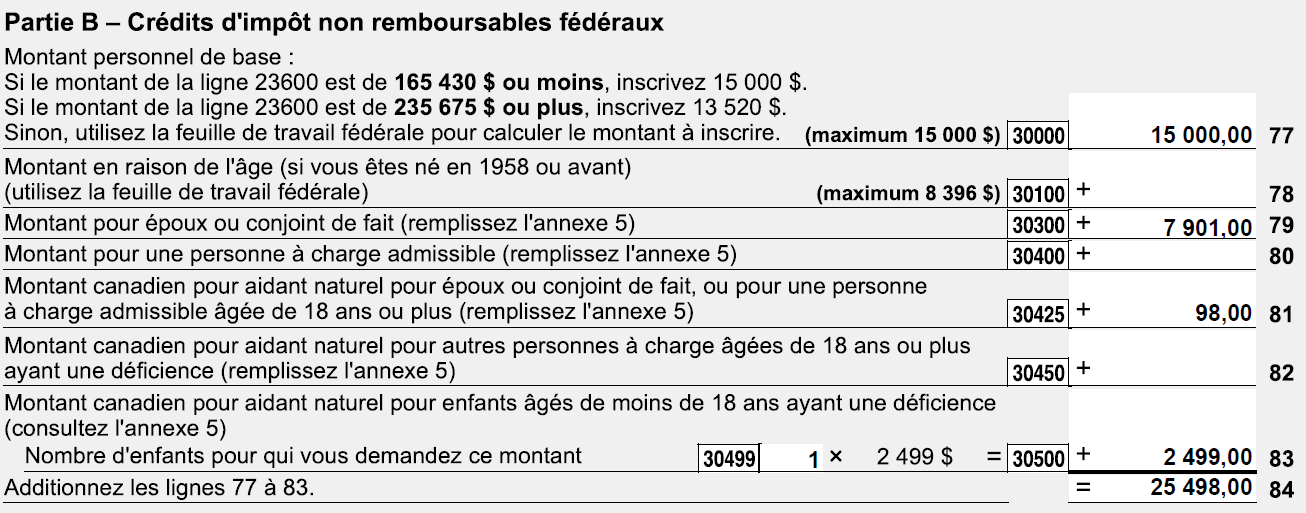
\includegraphics[width=.9\textwidth]{exercice/4-2/Q1/T1PartieB.png}
	\caption[]{Exercice 2, T1, partie~B}
	\label{fig:chap4Exercice2Q1T1B}
\end{figure}

\begin{question}
	Elaine et Suzie subviennent toutes deux aux besoins de leur sœur Janet, âgée de 15~ans. Les trois sœurs vivent dans le même logement. 
	
	Elaine et Suzie peuvent-elles toutes deux demander un montant pour personne à charge admissible pour Janet? Peuvent-elles partager ce montant? Expliquez votre réponse.
\end{question}
Non. Un seul montant pour une personne à charge éligible peut être demandé par personne à charge et par logement. Elaine et Suzie ne peuvent pas se partager le montant. Elles doivent décider laquelle d'entre elles demandera le montant.

\begin{question}
	Sophie est célibataire. Elle a la garde légale de son neveu de trois ans, dont elle subvient aux besoins comme si c'était son enfant. 
	
	Est-ce que Sophie peut réclamer le montant pour une personne à charge admissible à l'égard de son neveu, même si ce dernier n'est pas légalement son enfant adoptif?
\end{question}
Oui. Il n'est pas nécessaire que l'enfant soit adopté légalement pour être considéré comme l'enfant d'un contribuable.

\begin{question}
	Durant toute l'année, John a vécu avec sa mère. Elle est veuve et son revenu net est de \numprint{5809}~\$, au fédéral.
\end{question}
\setcounter{sousQuestion}{0}
\begin{sousQuestion}
	Sous quelles conditions John peut-il réclamer le montant pour une personne à charge admissible à l'égard de sa mère?
\end{sousQuestion}
John peut réclamer le montant pour une personne à charge admissible à l'égard de sa mère seulement s'il n'a pas vécu avec une conjointe (épouse ou de fait) une partie de l'année. Toutefois, il ne doit pas avoir de conjointe (épouse ou de fait) au 31~décembre de l'année d'imposition.

Si John est séparé au 31~décembre de l'année d'imposition, son ex-conjointe ne peut pas être à sa charge. Il ne peut pas non plus être à la charge de son ex-conjointe.

Sa mère ne peut être considérée comme une personne à charge par aucun autre contribuable. Personne d'autre dans le logement ne peut demander un montant pour une personne à charge admissible.

\begin{sousQuestion}
	Si John peut réclamer le montant pour une personne à charge admissible à l'égard de sa mère, quel montant peut-il réclamer sur son annexe~5 et qui sera reporté à la ligne~30400 de sa T1?
\end{sousQuestion}
Le montant personnel de base que John peut réclamer selon son revenu net moins le revenu net de sa mère.

\begin{question}
	Leslie a vécu jusqu'au jour de son 18e anniversaire, qui a eu lieu en septembre 2023, chez son père qui est veuf. Elle s'est ensuite mariée avec Robert en octobre et vit avec celui-ci depuis ce temps.
	
	Le père de Leslie veut réclamer le montant pour personne à charge admissible pour sa fille. Robert veut réclamer le montant pour époux ou conjoint de fait pour son épouse.
	
	Lequel des deux, entre le père de Leslie et Robert, a préséance pour réclamer un montant concernant Leslie? Les deux peuvent-ils réclamer un montant? Expliquez votre réponse.
\end{question}
Les deux peuvent réclamer le montant auquel ils ont droit.

Il n'est pas nécessaire d'avoir la charge d'une personne toute l'année pour réclamer le crédit.

Dans les deux cas, le revenu net de Leslie affectera le montant réclamé.

\begin{question}
	Daniel Duval est divorcé depuis deux ans. Il a la garde de ses deux enfants: Simon, avec le NAS 801-115-353 est né le 16 août 2006 (17~ans) et Alicia, avec le NAS 801-115-361 est née le 2 février 2009 (14~ans).
	
	Le revenu net de Simon est de \numprint{2850}~\$ et celui de Alicia, de 300~\$. Le crédit d'impôt \og Montant personnel de base \fg{} de Daniel est \numprint{15000}~\$.
	
	Daniel et les enfants vivent au 92 rue Barlow, Québec, QC, G1C 3L5.
	
	En supposant que Daniel puisse demander le montant pour une personne à charge admissible, préparez la partie ligne~30400 de l'\href{https://www.canada.ca/fr/agence-revenu/services/formulaires-publications/trousses-impot-toutes-annees-imposition/trousse-generale-impot-prestations/5000-s5.html}{annexe~5} en choisissant l'enfant qui fournira la demande la plus avantageuse.
\end{question}
Il est plus avantageux pour Daniel de réclamer l'enfant qui a le revenu net le moins élevé (Alicia).

Il peut ainsi réclamer \numprint{14700}~\$ (\numprint{15000}~\$ – 300~\$).

La ligne~\og 30400 \fg{} de l'annexe~5 de Daniel: figure~\ref{fig:chap4Exercice2Q6}.
\begin{figure}
	\centering
	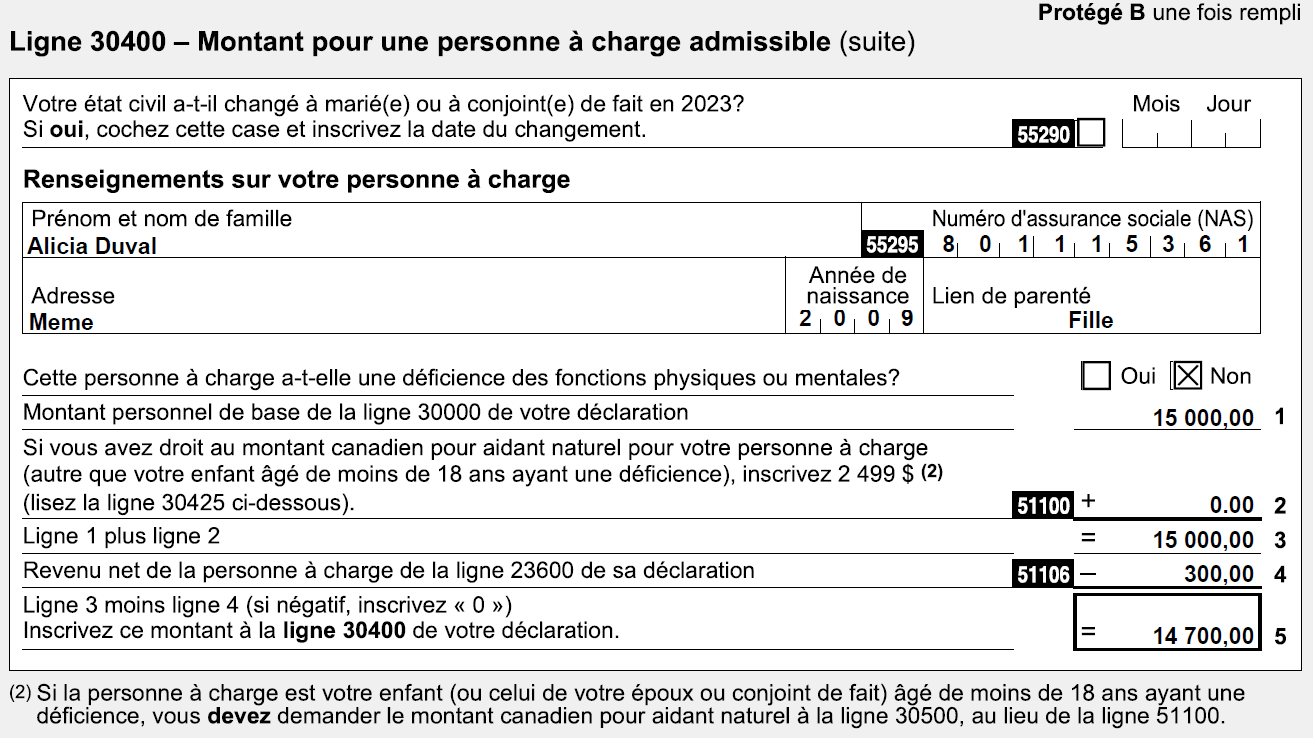
\includegraphics[width=.9\textwidth]{exercice/4-2/Q6/30400.png}
	\caption[]{Exercice 2, Q6, annexe~5, ligne~30400}
	\label{fig:chap4Exercice2Q6}
\end{figure}

\begin{question}
	Supposons que Alicia, de la question \og Q6 \fg{}, souffre d'une déficience mentale attestée par son médecin. Elle étudie dans une école spécialisée pour déficients intellectuels.
	
	Complétez l'\href{https://www.canada.ca/fr/agence-revenu/services/formulaires-publications/trousses-impot-toutes-annees-imposition/trousse-generale-impot-prestations/5000-s5.html}{annexe~5} et les lignes correspondantes de la \href{https://www.canada.ca/fr/agence-revenu/services/formulaires-publications/trousses-impot-toutes-annees-imposition/trousse-generale-impot-prestations/quebec/5005-r.html}{T1} (Partie B de l'étape 5) de Daniel de la façon la plus avantageuse. 
	
	Utilisez les renseignements relatifs, à la question Q6.
\end{question}
Si Alicia est handicapée, Daniel peut demander le montant canadien pour aidants naturels. Il devrait demander le montant canadien pour aidants naturels pour enfants de moins de 18~ans ayant une déficience à la ligne~30500 et non à la ligne~30400, car Alicia est mineure.

Ainsi, la grille de calcul pour la ligne~30400 sera la même qu'à la question 6, sauf que Daniel devra répondre \og Oui\fg{} à la question \og Cette personne à charge a-t-elle une déficience des fonctions mentales ou physiques?\fg{}

Section \og ligne~30400 - Montant pour une personne à charge admissible \fg{},5005-R F, page 4: figure~\ref{fig:chap4Exercice2Q7S5}.
\begin{figure}
	\centering
	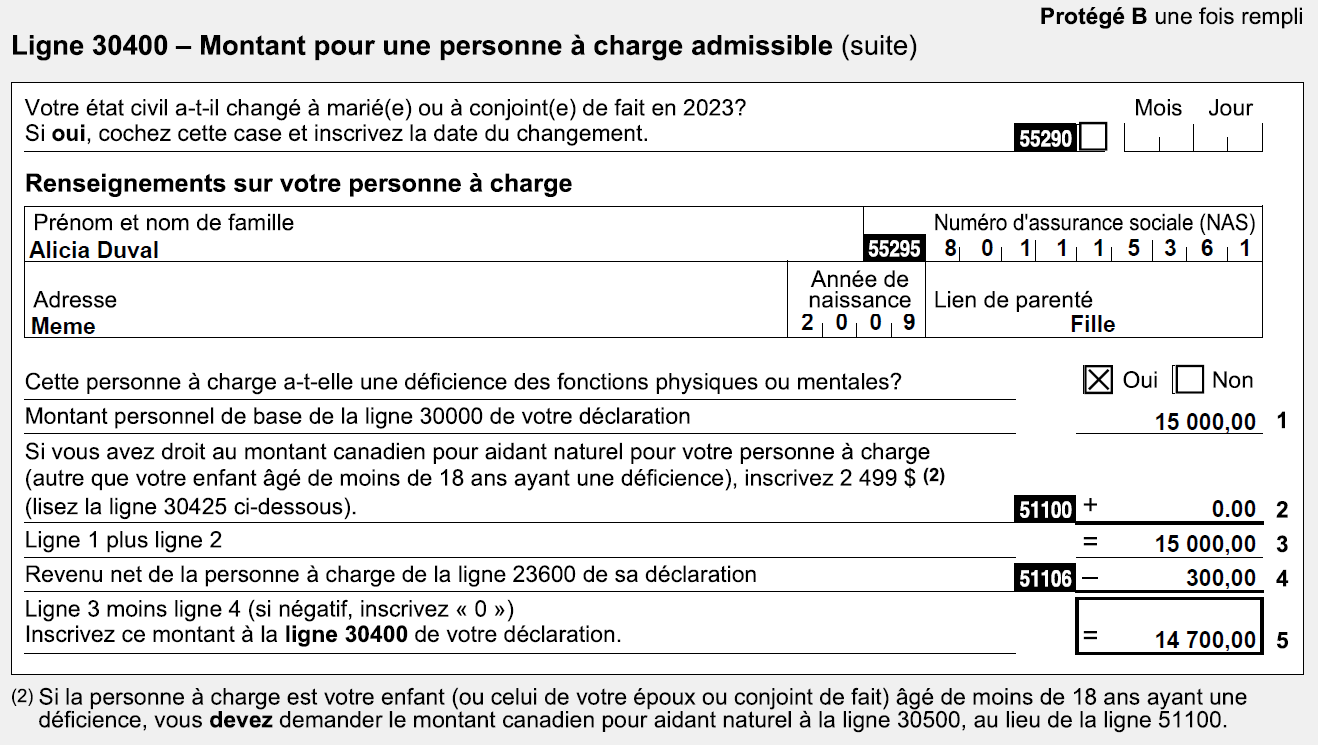
\includegraphics[width=.9\textwidth]{exercice/4-2/Q7/30400.png}
	\caption[]{Exercice 2, Q7, annexe~5, ligne~30400}
	\label{fig:chap4Exercice2Q7S5}
\end{figure}

Daniel demande le montant pour personne à charge admissible pour Alicia. Cependant, le Montant canadien pour aidant naturel n'est pas réclamé à la ligne~30400, mais à la ligne~30500: figure~\ref{fig:chap4Exercice2Q7T1}.
\begin{figure}
	\centering
	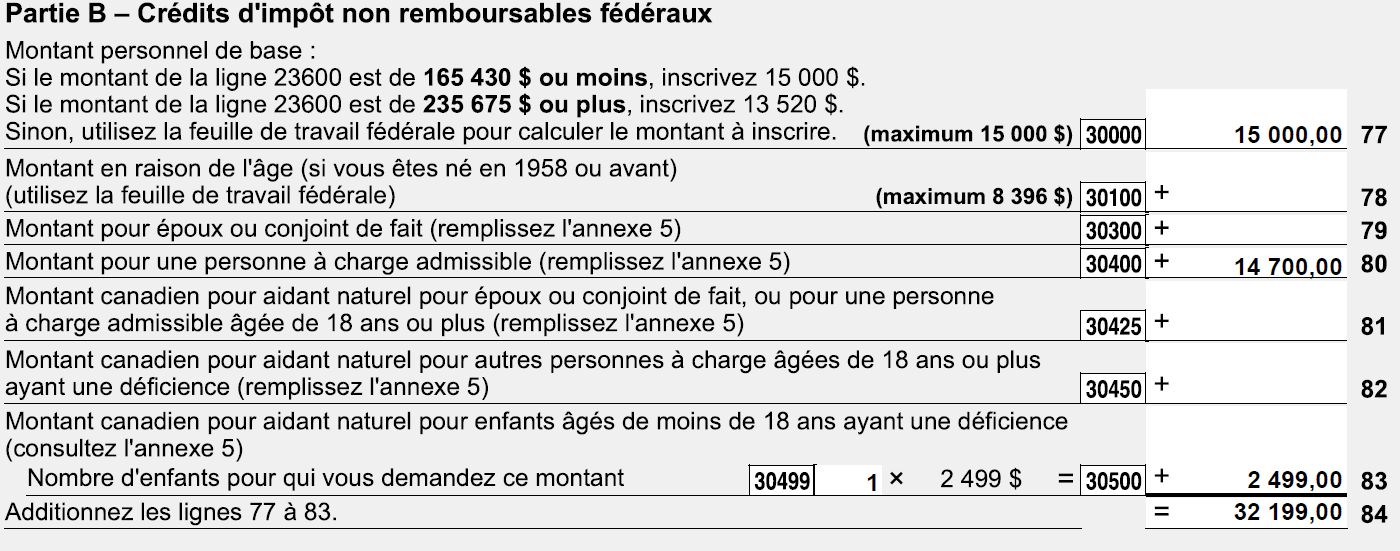
\includegraphics[width=.9\textwidth]{exercice/4-2/Q7/T1.png}
	\caption[]{Exercice 2, Q7, T1}
	\label{fig:chap4Exercice2Q7T1}
\end{figure}

\begin{question}
	Durant toute l'année, Paolo a vécu avec sa mère âgée de 55~ans, qui est sans revenu. Elle a une bonne santé. Paolo subvient aux besoins de sa mère.
\end{question}
\setcounter{sousQuestion}{0}
\begin{sousQuestion}
	Quel montant personnel Paolo, qui est célibataire, peut-il demander pour sa mère sur sa déclaration fédérale?
\end{sousQuestion}
Paolo peut demander le montant pour une personne à charge admissible.

Il doit utiliser la ligne~30400 de l'annexe~5 pour calculer le montant qu'il peut demander.

\begin{sousQuestion}
	Si Paolo a été marié durant toute l'année, quel montant personnel pourrait-il réclamer pour sa mère?
\end{sousQuestion}
Aucun.

Cependant, si sa mère avait souffert d'une déficience physique ou mentale, Poalo aurait pu réclamer le montant canadien pour aidant naturel pour autres personnes à charge âgées de 18~ans ou plus ayant une déficience à la ligne~30450 .

\begin{question}
	Jean et Marguerite sont mariés. Ils subviennent tous les deux aux besoins du frère de Jean, Tommy, âgé de 20~ans, qui souffre d'une déficience mentale. 
	
	Tommy a un revenu net de \numprint{15000}~\$ en 2023 et il vit seul. Jean et Marguerite peuvent réclamer le montant canadien pour aidant naturel pour autres personnes à charge âgées de 18~ans ou plus ayant une déficience. Ils veulent diviser le montant admissible entre eux. 
	
	Quel est le montant que Jean et Marguerite peuvent chacun réclamer? Expliquez vos calculs.
\end{question}
Jean et Marguerite peuvent réclamer chacun \numprint{3999,50}~\$ (\numprint{7999}~\$ $\times$ 50~\%).

\begin{question}
	Nathalie Angers et son conjoint de fait, Bruce Watson, subviennent aux besoins du père de Nathalie, Grégoire Angers, qui est confiné au lit dans un Centre d'hébergement et de soins de longue durée situé au 38, rue Sauvé, Alma, QC. Grégoire a un revenu net de \numprint{6422}~\$. Il est né le 1er juillet 1959 (64~ans). Personne d'autre n'a réclamé un montant personnel à l'égard de Grégoire.
	
	Quel montant personnel Natalie ou Bruce peuvent-ils demander à l'égard de Grégoire?
\end{question}
Comme Natalie et Bruce soutiennent Grégoire pendant qu'il est dans un Centre d'hébergement et de soins de longue durée, ils peuvent demander le montant canadien pour aidant naturel pour d'autres personnes à charge âgées de 18~ans ou plus et ayant une déficience.

\begin{question}
	André et Jocelyne Malouin pourvoient aux besoins de la mère de André, Mariette, qui vit avec eux. Mariette est née le 13 juin 1951 (72~ans) et a un revenu net de \numprint{18961}~\$. Elle a une déficience physique, attestée par son médecin.
\end{question}
\setcounter{sousQuestion}{0}
\begin{sousQuestion}
	Calculez le Montant canadien pour aidant naturel pour autres personnes à charge âgées de 18~ans ou plus ayant une déficience, que le couple peut réclamer. Utilisez la partie \og ligne~30450 \fg{} de l'\href{https://www.canada.ca/fr/agence-revenu/services/formulaires-publications/trousses-impot-toutes-annees-imposition/trousse-generale-impot-prestations/5000-s5.html}{annexe~5}.
\end{sousQuestion}
Notez que la ligne~51120 doit être remplie dans la grille de calcul. Dans cet exemple, une seule personne à charge est déclarée.

ligne~30450:
figure~\ref{fig:chap4Exercice2Q11}.
\begin{figure}
	\centering
	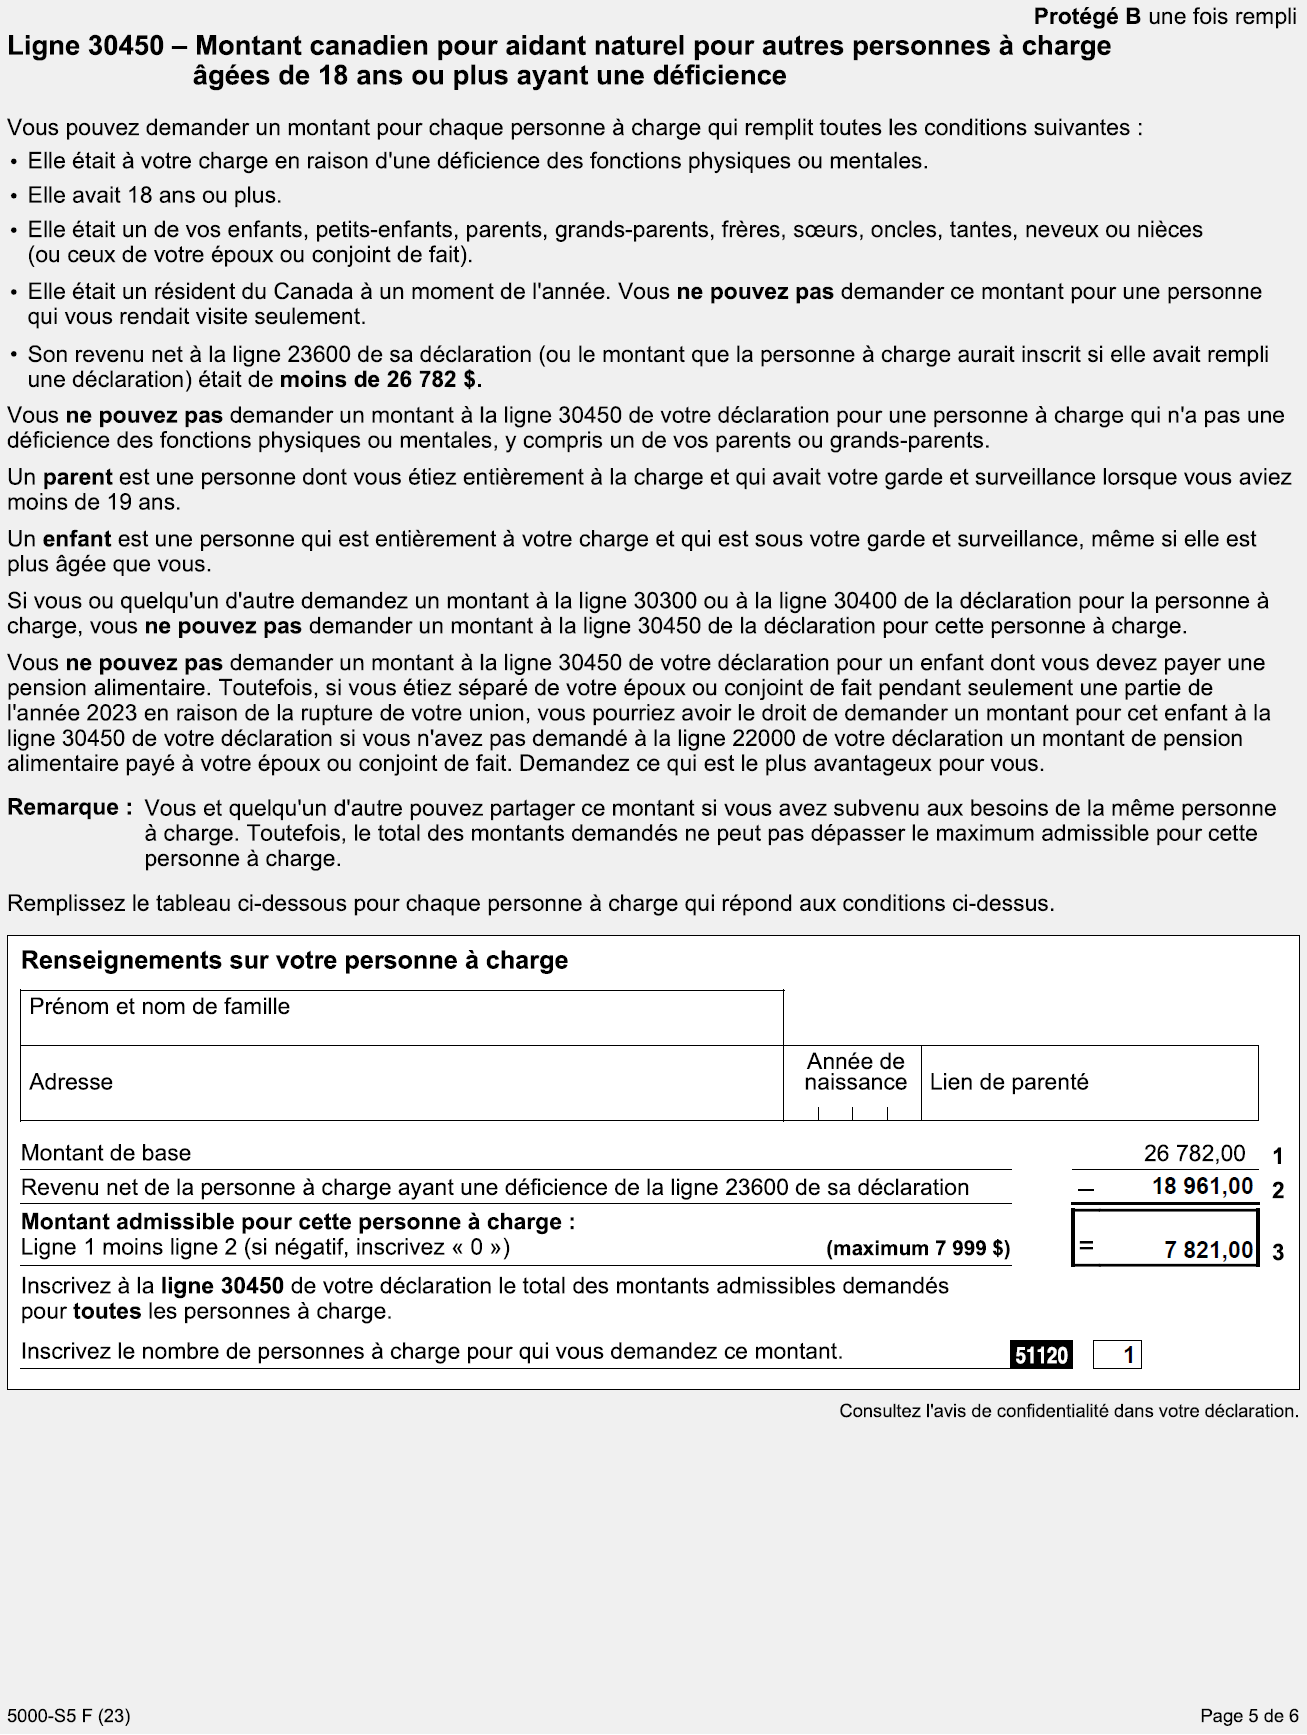
\includegraphics[width=.9\textwidth]{exercice/4-2/Q11/30450.png}
	\caption[]{Exercice 2, annexe~5, ligne~30450}
	\label{fig:chap4Exercice2Q11}
\end{figure}

\begin{sousQuestion}
	Qui peut réclamer ce montant?
\end{sousQuestion}
André ou Jocelyne peuvent réclamer le montant total du crédit ou se le partager, tant et aussi longtemps que les montants partagés n'excèdent pas \numprint{7821}~\$.



\section{Crédit pour la TPS/TVH}
\begin{intro}
	Le crédit pour la taxe sur les produits et services (TPS) est un montant non imposable (fédéral ou Québec). Il aide les particuliers et les familles à revenu faible ou modeste pour compenser la taxe sur les produits et services/taxe de vente harmonisée (TPS/TVH) qu'ils paient.
\end{intro}

Dans la discussion qui suit, l'acronyme TPS signifie TPS/TVH.

Le crédit de TPS est payé en quatre versements égaux, c'est-à-dire le premier versement en juillet, les autres versements étant effectués sur une base trimestrielle en octobre, janvier et avril.


\subsection{Admissibilité}
Pour être admissible au crédit pour la TPS, le contribuable doit être résident du Canada au début du mois où le paiement est fait et il doit répondre à l'une des conditions suivantes:
\begin{itemize}
	\item Avoir 19~ans ou plus;
	\item Avoir (ou avoir eu) un époux ou un conjoint de fait; ou
	\item Être (ou avoir été) le parent d'un enfant avec qui il habite (ou habitait).
\end{itemize}

Selon ces critères d'admissibilité, un contribuable de moins de 19~ans peut donc demander le crédit s'il a un époux ou conjoint de fait, ou s'il est le père ou la mère d'un enfant avec qui il habite (ou habitait).

Un contribuable ne peut pas recevoir le crédit pour la TPS si, au début du mois où un paiement est fait:
\begin{itemize}
	\item Il n'est pas un résident du Canada aux fins de l'impôt sur le revenu;
	\item Il est détenu dans une prison ou dans un établissement semblable pour une période d'au moins 90~jours consécutifs;
	\item Il n'est aucun impôt à payer au Canada, car il est soit un agent ou un fonctionnaire d'un gouvernement étranger (par exemple, un diplomate), soit un membre de sa famille ou l'un de ses employés;
	\item Le bénéficiaire est décédé.
\end{itemize}

De plus, il ne peut pas recevoir le crédit pour un époux, un conjoint de fait ou un enfant qui se trouve dans l'une des situations ci-dessus au début du mois où l'ARC effectue un versement.

\subsubsection{Personne qui aura 19~ans avant avril 2025}
Un contribuable est admissible à recevoir le crédit pour la TPS à compter du premier versement suivant le mois de son 19e anniversaire. 

Cela signifie que toute personne qui atteint 19~ans avant le 1er avril 2025 pourra se qualifier pour au moins un versement s'il remplit les autres conditions d'admissibilité. 

Pour recevoir le crédit, ils doivent commencer à envisager de produire leur déclaration fédérale de 2023 à l'âge de 17~ans.


\subsection{Demande du crédit pour la TPS}
C'est l'Agence de revenu du Canada (ARC) qui détermine automatiquement l'admissibilité du contribuable suite à la production de sa T1.

Un contribuable seul, s'il est éligible, recevra son propre crédit de TPS.

Si un contribuable est marié ou a un conjoint de fait, un seul conjoint recevra le crédit au nom des deux. Celui qui recevra le paiement dépendra de la déclaration qui sera cotisée en premier, mais cela ne peut pas être garanti.

Les nouveaux arrivants au Canada doivent produire le formulaire \href{https://www.canada.ca/fr/agence-revenu/services/formulaires-publications/formulaires/rc151.html}{RC151}.

\begin{note}
	Vous remarquerez que le formulaire RC151 fait référence au paiement de l'Incitatif à agir pour le climat. Pour l'instant, le Québec ne participe pas à cette prestation fédérale.
\end{note}


\subsection{Calcul du crédit pour la TPS}
Le calcul du crédit pour la TPS ne figure nulle part sur la T1 ni dans le Guide d'impôt et de prestations fédéral. 

Le calcul du crédit pour la TPS se fait par le gouvernement fédéral et non pas par le contribuable.

\subsubsection{Année de base et année de prestations}
L'année de base est l'année de la déclaration de revenus et de prestations à partir de laquelle les renseignements sont tirés pour calculer les versements du crédit pour la TPS. L'année de base est l'année civile qui précède le début de l'année de prestations.

L'année de prestations est la période de 12 mois pendant laquelle le crédit pour la TPS est versé. Cette période suit l'année de base, débutant le 1er juillet et se terminant le 30 juin de l'année suivante. 

Par exemple, la production de la T1 de 2023 sert à établir les paiements devant être versés en juillet et octobre 2024 ainsi que ceux de janvier et avril 2025.


\subsection{Changement dans la situation familiale}
Le crédit pour la TPS peut être rajusté par l'ARC s'il y a eu un changement dans la situation familiale qui altère le calcul du montant du crédit. Le rajustement paraîtra sur le paiement du trimestre suivant. Les changements de situation familiale qui peuvent donner suite à un rajustement comprennent:
\begin{itemize}
	\item Un changement dans l'état civil;
	\item Un changement dans le nombre d'enfants;
	\item Le contribuable, son conjoint ou un enfant admissible décède;
	\item Le contribuable, son conjoint ou un enfant admissible cesse de résider au Canada.
\end{itemize}

Dans le cas d'un changement d'état civil, le contribuable doit informer l'ARC en remplissant le formulaire \href{https://www.canada.ca/fr/agence-revenu/services/formulaires-publications/formulaires/rc65.html}{RC65 -- Changement d'état civil}, ou en écrivant une lettre.

\begin{note}
	Si l'ARC n'est pas informé du changement d'état civil avant le trimestre suivant, il est possible que le contribuable qui s'est marié ou a débuté une union de fait ait à rembourser le paiement qu'il a reçu après le changement. 
\end{note}

\cat
Guide RC4210 \href{https://www.canada.ca/fr/agence-revenu/services/formulaires-publications/publications/rc4210.html}{Crédit pour la TPS/TVH} (13~pages)

\subsection{Remboursement pour l'épicerie}
Pour aider à faire face à la hausse des coûts d'épicerie, un remboursement unique sur l'épicerie a été émis le 5 juillet 2023, en même temps que le paiement trimestriel du crédit pour la TPS/TVH de juillet 2023.

Pour obtenir le remboursement pour l'épicerie, il faut produire une déclaration de revenus de 2021, même s'il n'avait aucun revenu à déclarer pour cette année.

\cat \href{https://www.canada.ca/fr/agence-revenu/services/prestations-enfants-familles/credit-taxe-produits-services-taxe-vente-harmonisee-tps-tvh/credit-tps-tvh-feuilles-calcul.html}{Crédit pour la TPS/TVH: feuilles de calcul}



\section{Allocation canadienne pour enfants (ACE)}
\begin{intro}
	L'\acrfull{ace} est un programme géré par l'Agence du revenu du Canada (ARC). Il s'agit d'une prestation non imposable versée aux familles à faibles et moyens revenus ayant des enfants.
\end{intro}

Les montants versés dans le cadre de l'ACE varient en fonction:
\begin{enumerate}
	\item Du nombre d'enfants 
	\item De l'âge des enfants 
	\item Du revenu net familial (célibataire ou en couple).
\end{enumerate}

Étant donné que le montant de l'Allocation canadienne pour enfants est basé sur le revenu, les contribuables doivent produire des déclarations de revenus pour la recevoir. Si une personne est mariée ou vit en union de fait, les deux conjoints doivent produire des déclarations.

\begin{note}
	L'ARC retiendra ou retardera les paiements de l'ACE si l'un des parents ou les deux ont omis ou retardé de produire leur déclaration de revenus T1.
\end{note}

Les prestations versées ne sont pas imposables. Elles ne doivent pas être incluses dans les revenus, tant au fédéral qu'au Québec.


\subsection{Admissibilité}
Pour recevoir l'ACE à l'égard d'un enfant, le contribuable doit satisfaire à toutes les conditions suivantes:
\begin{enumerate}
	\item Habite avec un enfant de moins de 18~ans;
	\item être le principal responsable des soins et de l'éducation de l'enfant. Cette personne est responsable pour des chose telles que:
	\begin{enumerate}
		\item supervise les activités et répondre aux besoins de l'enfant au quotidien;
		\item veille à ce que l'enfant reçoive les soins médicaux nécessaires;
		\item trouve quelqu'un pour s'occuper de l'enfant lorsque requis.
		\item Lorsqu'un parent féminin vit avec l'enfant
		\begin{enumerate}
			\item Lorsque deux individus mariés ou conjoint de fait résident au même domicile que l'enfant, le parent féminin est présumée être le principal responsable des soins et de l'éducation de tous les enfant du ménage. Celle-ci devrait être celle qui fait la demande d'ACE. La présomption en faveur du parent féminin est une exigence législative et un seul versement par ménage peut être émis en vertu de la Loi sur l'impôt sur le revenu. Peu importe quel parent reçoit l'ACE, le montant sera le même.
			\item Toutefois, si l'autre parent est le principal responsable, il devrait faire une demande et y joindre une lettre signée du parent féminin qui indique qu'il est le principal responsable des soins et de l'éducation de tous les enfants du ménage.
			\item Si l'enfant réside avec des parents du même sexe, un seul des parents doit présenter une demande pour tous les enfants habitant la même maison.
		\end{enumerate}
	\end{enumerate}
	\item Ils doivent être résidents du Canada aux fins de l'impôt
	\begin{enumerate}
		\item Il doit s'agir de l'un des éléments suivants:
		\begin{enumerate}
			\item Être citoyen canadien;
			\item Selon la Loi sur l'immigration et la protection des réfugiés:
			\begin{enumerate}
				\item être citoyen canadien;
				\item un résident permanent;
				\item une personne protégée;
				\item un résident temporaire qui a habité au Canada pendant les 18 mois qui précèdent la demande et qui possède un permis valide au 19e mois autre qu'un permis avec la mention \og ne confère pas de statut \fg{} ou \og ne confère pas le statut de résident temporaire \fg{}
				\item une personne qui est inscrite ou qui a le droit d'être inscrite en vertu de la Loi sur les Indiens
			\end{enumerate}
		\end{enumerate}
	\end{enumerate}
\end{enumerate}

Au Québec, les mères peuvent demander l'ACE et toutes autres prestations provinciales connexes au moment de la naissance, en indiquant sur le formulaire d'enregistrement de naissance qu'elles consentent à ce que le bureau de l'état civil provincial partage les renseignements avec l'ARC.


\subsection{Enfant admissible}
Un enfant est admissible à l'Allocation canadienne pour enfants si toutes les conditions suivantes sont satisfaites:
\begin{itemize}
	\item Il est âgé de moins de 18~ans au début du mois du versement de la prestation;
	\item Personne n'a demandé un montant pour époux ou conjoint de fait à son égard durant l'année de base;
	\item Aucune allocation spéciale n'a été versée au nom de l'enfant en vertu de La Loi sur les allocations spéciales pour enfants.
\end{itemize}

\begin{note}
	Un enfant admissible ne comprend pas un enfant qui vit dans une famille d'accueil ni un enfant qui n'est pas sous la garde des parents. Les parents doivent vivre avec l'enfant pour pouvoir recevoir l'ACE.
\end{note}

Si un enfant de moins de 18~ans est marié et que le couple demeure chez les parents de l'enfant, ce dernier (l'enfant) est admissible à l'ACE si son époux ne réclame pas le montant pour époux ou conjoint de fait à son égard. Il est possible de recevoir l'ACE pour un enfant à l'égard duquel on réclame un montant pour une personne à charge admissible.


\subsection{Calcul de l'allocation canadienne pour enfants}
Le calcul de l'ACE se fait par le gouvernement fédéral et non pas par le contribuable.

\subsubsection{Revenu net, rajusté de la famille}
Le calcul du montant de l'ACE tient compte du revenu familial net
rajusté, soit:
\begin{itemize}
	\item Le revenu net du contribuable et celui de son époux ou conjoint de fait, inscrit à la ligne~23600 de leur T1; plus
	\item Le remboursement de la prestation universelle pour la garde d'enfants, ligne~21300 de la T1 du contribuable ou de celle de son époux ou conjoint de fait; plus
	\item Le remboursement des revenus d'un régime enregistré d'épargne-invalidité, ligne~23200 de la T1 du contribuable ou de celle de son époux ou conjoint de fait; moins
	\item La prestation universelle pour la garde d'enfants, qui est déclarée à la ligne~11700 de la déclaration T1 du contribuable ou de celle de son époux ou conjoint de fait; moins
	\item Le revenu d'un régime enregistré d'épargne-invalidité déclaré à la ligne~12500 de la déclaration T1 du contribuable ou de celle de son époux ou conjoint de fait.
\end{itemize}

\subsubsection{Année de base et année de l'allocation}
Tout comme le crédit pour la TPS, le montant que les contribuables recevront à partir de juillet 2024 à juin 2025 est calculé en tenant compte de l'année de base de 2023. 

\begin{rappel}
	L'année de base est l'année de la déclaration de revenus fédérale. C'est donc l'année civile qui précède le début de l'année de prestations. L'année de prestations débute le 1er juillet de l'année qui suit l'année de base et se termine le 30 juin de la deuxième année suivant l'année de base
\end{rappel}.

\subsubsection{Calcul de l'allocation}
\cat\href{https://www.canada.ca/fr/agence-revenu/services/prestations-enfants-familles/calculateur-prestations-enfants-familles.html}{Calculateur de prestations pour enfants et familles}


\subsection{Prestation pour enfants handicapés (PEH)}
En plus de la prestation de base, le contribuable peut demander la \acrfull{peh} pour aider sa famille à subvenir aux besoins d'un ou des enfants admissible(s) au montant pour déficience mentale ou physique grave et prolongée.

Le contribuable peut demander la PEH s'il a un enfant âgé de moins de 18~ans qui a droit au montant pour personnes handicapées. 

\cat
Livret T4114 \href{https://www.canada.ca/fr/agence-revenu/services/formulaires-publications/publications/t4114.html}{Allocation canadienne pour enfants et les programmes provinciaux et territoriaux connexes} (15 pages)



\section{Crédits d'impôt non remboursables au fédéral}
\begin{intro}
	Les crédits d'impôt non remboursables ont pour but d'accorder aux contribuables un allègement fiscal pour le coût de la vie pour eux-mêmes et les personnes à leur charge. Ils réduisent le montant de l'impôt fédéral à payer jusqu'à concurrence du montant de l'impôt dû.
\end{intro}

Le résultat obtenu sur la ligne~100, peut être utilisé dans le calcul d'un crédit sur une autre ligne.

Le taux de 15~\% est appliqué. 


Si le total des crédits non remboursables est plus élevé que l'impôt à payer, la différence n'est pas remboursée, d'où le nom de crédits d'impôt \textbf{non remboursables}.



\section{Exercice 3}
\setcounter{question}{0}
\begin{question}
	Qui a droit au crédit pour la TPS/TVH?
\end{question}
Une des conditions suivantes doit être respectée:
\begin{itemize}
	\item Un résident du Canada âgé de 19~ans ou plus;
	\item Un contribuable canadien qui a un époux ou un conjoint de fait; ou
	\item Un contribuable canadien qui est parent d'un enfant avec lequel il habite (habitait).
\end{itemize}

\begin{question}
	Dans le cas d'un couple marié ou de conjoints de fait, qui doit demander le crédit pour la TPS/TVH lorsqu'il produit sa déclaration T1?
\end{question}
Dans un couple, un ou l'autre des conjoints peut recevoir le crédit pour la famille. Même si le couple n'a pas à déposer une demande pour le crédit TPS, les deux doivent produire leur T1.

Bien que la notion qui court, indiquant que la première déclaration transmise à l'ARC donne au contribuable de meilleures chances d'obtenir le crédit, il n'y a aucune garantie de succès dans cette pensée.

Selon l'ARC, \og La cotisation comprend des procédures internes qui ne reposent pas sur la séquence de production. Bien que les situations soient fréquentes où l'ordre de cotisation s'alignera avec l'ordre de production initiale, l'application de ces procédures est telle que l'ordre de cotisation ne peut être basée avec certitude sur l'ordre de production. \fg{}

\begin{question}
	Johanne a eu 19~ans le 22 avril 2024. Elle est célibataire.
	
	Que doit-elle faire pour recevoir pour la première fois le crédit pour la TPS?
\end{question}
Si Johanne a eu 19~ans le 22 avril 2024, cette date la rendrait éligible à recevoir la TPS dès juillet 2024. Par contre, pour réclamer la TPS dès juillet 2024, il faut qu'elle ait produit sa déclaration 2023.

Même si elle n'avait que 18~ans le 31~décembre~2023, il fallait produire la T1 pour, lorsqu'elle aurait 19~ans en avril, qu'elle soit en droit de recevoir le crédit TPS.

Autre situation (un peu plus compliqué).

Si Johanne avait eu 19~ans en février 2024, quel serait votre raisonnement pour qu'elle reçoive son crédit TPS en avril 2024?

Réponse. Elle aurait produit sa déclaration de 2022 même si elle n'avait que 17~ans. En effet, en produisant sa T1 de 2022, le premier versement aurait été dû en juillet 2023 pour se terminer en juin 2024. Or, elle a eu 19~ans seulement en février 2024, elle aurait donc pu réclamer le crédit de la TPS/TVH du mois d'avril 2024.

\begin{question}
	Catherine Spencer, avec le NAS 801 115 379, a eu 17~ans le 20~décembre~2023. Elle demeure avec sa fille Céleste, qui est née le 2 mai 2023. Catherine réclame un montant pour une personne à charge admissible à l'égard de sa fille. Elle ne vivait pas avec le père de son enfant à la fin de l'année. Le revenu net de Catherine est de \numprint{26700}~\$.
	
	A-t-elle droit au crédit pour la TPS/TVH? Expliquez votre réponse.
\end{question}
Bien qu'elle soit âgée de moins de 19~ans, Catherine Spencer est admissible au crédit pour la TPS, parce qu'elle est le parent d'un enfant.

Comme sa fille est né en mai 2023, elle est admissible au premier versement de la TPS à compter de Juillet 2023. Si elle n'a pas produit de déclaration de revenus pour 2022, elle devrait le faire pour recevoir les paiements rétroactifs à partir de juillet 2023.

Vous devez produire vos déclarations d'impôts afin de recevoir le crédit de taxes (TPS) et l'allocations pour enfants canadienne. 

\begin{question}
	Élizabeth est âgée de 16~ans. Elle est la mère d'un enfant de 5 mois. Élizabeth et son enfant demeurent chez Barbara, la mère de Élizabeth. Ils sont à la charge de Barbara, qui a réclamé le montant pour une personne à charge admissible à l'égard de l'enfant de Élizabeth sur sa T1.
\end{question}
\setcounter{sousQuestion}{0}
\begin{sousQuestion}
	Est-ce que Élizabeth peut recevoir le crédit pour la TPS pour elle-même et son enfant? Expliquez votre réponse.
\end{sousQuestion}
Oui. Élizabeth est le parent d'un enfant et ce dernier est un enfant admissible. Elle doit produire une déclaration de revenus.

\begin{sousQuestion}
	Est-ce que Barbara peut recevoir le crédit pour la TPS pour Élisabeth? Expliquez votre réponse.
\end{sousQuestion}
Non. Élizabeth n'est plus un enfant admissible pour Barbara, car Élisabeth est elle-même le parent d'un enfant admissible et a droit de recevoir son propre crédit pour la TPS/TVH.

\begin{question}
	David et Martin sont mariés et ont trois enfants âgés respectivement de 6, 12 et 17~ans. Aux fins de l'allocation canadienne pour enfants:
\end{question}
\setcounter{sousQuestion}{0}
\begin{sousQuestion}
	Doivent-ils informer l'ARC lorsque l'enfant de 6~ans atteindra sa 7e année et lorsque celui âgé de 17~ans aura 18~ans?
\end{sousQuestion}
Non. Ces rajustements sont faits automatiquement, basés sur la date de naissance de l'enfant.

\begin{sousQuestion}
	Doivent-ils informer l'ARC si l'enfant de 17~ans quitte la maison?
\end{sousQuestion}
Oui. L'ARC ne pourra pas savoir à quel moment un enfant n'est plus admissible, parce qu'il ne vit plus avec ses parents. Donc, c'est aux parents ou à l'enfant d'aviser l'ARC.



\section{Allocation famille -- Québec}
\begin{intro}
	Le paiement de soutien aux enfants est une aide financière versée par Retraite Québec à toutes les familles qui ont des enfants à charge de moins de 18~ans qui résident avec elles.
\end{intro}

À la naissance d'un enfant, son inscription au programme \og Soutien pour enfants \fg{} est faite par le directeur de l'état civil du Québec. Ce dernier avise Retraite Québec de la naissance de l'enfant. Le paiement de l'allocation famille est fait à une seule personne par famille. Les conjoints peuvent toutefois décider qui recevra le paiement pour l'ensemble des enfants. 


\subsection{Supplément pour enfant handicapé}
Il n'est pas réduit en fonction du revenu de la famille de l'enfant et il n'est pas imposable.

\subsubsection{Supplément pour enfant handicapé nécessitant des soins exceptionnels (SEHNSE)}
Le \acrfull{sehnse} est une prestation supplémentaire pour un enfant pour les parents qui reçoivent déjà l'allocation famille et le supplément pour enfants handicapés. Il est structuré en deux paliers selon que l'enfant souffre d'handicaps graves et multiples ou nécessite des soins médicaux complexes à domicile.


\subsection{Supplément pour l'achat de fournitures scolaires}
Le supplément pour l'achat de fournitures scolaires s'adresse aux parents qui ont un enfant âgé de 4 à 16~ans au 30 septembre et qui sont admissibles à l'allocation famille.


\subsection{Versement des paiements pour l'allocation famille}
Quel que soit son revenu familial, une famille est assurée de recevoir le paiement de l'allocation famille. Même si le montant varie selon le revenu familial, il y a un montant maximum, mais aussi un montant minimum.

Comme pour l'ACE et la TPS, il est important de signaler tout changement de situation familiale à Retraite Québec ou la personne pourrait être responsable d'un remboursement des sommes versées après le changement.



\section{Crédit d'impôt pour solidarité}
\begin{intro}
	Le crédit d'impôt pour la solidarité est un crédit remboursable après impôt qui offre une aide accrue aux personnes et aux familles à faible revenu et qui vise à alléger les coûts associés à la TVQ et au logement. Il reconnaît également que les habitants des villages nordiques doivent supporter un coût de la vie plus élevée qu'ailleurs.
	
	Le crédit est réduit à zéro si le revenu familial dépasse le revenu familial maximum qui est calculé en fonction de la situation familiale du contribuable, c'est-à-dire s'il a un conjoint ou non et s'il a des enfants mineurs à charge.
\end{intro}

\qct\href{https://www.revenuquebec.ca/fr/citoyens/credits-dimpot/credit-dimpot-pour-solidarite/calcul-du-credit-dimpot-pour-solidarite/}{Calcul du crédit d'impôt pour solidarité}


\subsection{Admissibilité au crédit d'impôt pour solidarité}
Pour être admissible au \acrfull{cis}, le contribuable doit se conformer à toutes conditions suivantes:
\begin{itemize}
	\item Le contribuable est âgé de 18~ans et plus à la fin de l'année d'imposition;
	\item Le contribuable est âgé de moins de 18~ans, mais il est dans l'une des situations suivantes:
	\begin{itemize}
		\item il a un conjoint;
		\item il est le parent d'un enfant qui réside avec lui;
		\item il est un mineur émancipé reconnu par une autorité compétente.
	\end{itemize}
	\item Le contribuable réside au Québec;
	\item Le contribuable ou sa conjointe (épouse ou de fait):
	\begin{itemize}
		\item a la citoyenneté canadienne;
		\item selon la Loi sur l'immigration et la protection des réfugiés:
		\begin{itemize}
			\item est un \og résident permanent \fg{};
			\item est une \og personne protégée \fg{};
			\item est un \og résident temporaire \fg{} qui a habité au Canada pendant les 18 derniers mois.
		\end{itemize}
	\end{itemize}
\end{itemize}

\begin{note}
	Même s'ils sont éligibles, les contribuables doivent s'être inscrits au dépôt direct pour recevoir les paiements du CIS. Revenu Québec n'émet pas de chèques pour le paiement du CIS.
\end{note}

\begin{note}
	Le statut du contribuable au 31~décembre détermine le montant du CIS pour l'année de prestation suivante. Les changements ultérieurs ne seront pas pris en compte avant le 31~décembre suivant.
\end{note}


\subsection{Inéligibilité}
Les contribuables qui remplissent les conditions susmentionnées peuvent être inadmissibles s'ils ont été:
\begin{itemize}[label=\twemoji{cross mark}]
	\item Emprisonné au 31~décembre de l'année d'imposition ou, au cours de l'année d'imposition, emprisonné pour une durée cumulée de plus de 183~jours 
	\item Bénéficiaire de l'Allocation famille au 31~décembre de l'année d'imposition;
	\item Demandeur d'asile au 31~décembre de l'année d'imposition. 
\end{itemize}


\subsection{Demander le Crédit d'impôt pour solidarité}
Une seule demande de crédit d'impôt pour solidarité peut être faite par famille.

Si un enfant adulte, c'est-à-dire âgé de plus de 18~ans, vit toujours avec ses parents, il peut demander son propre CIS.

Chaque demande est effectuée en remplissant et en soumettant l'annexe~D avec la TP-1.

Ce crédit comporte trois composantes principales. Si le contribuable a droit au crédit, mais qu'il ne remplit pas l'annexe~D et ne la joint pas à son formulaire TP-1 comme recommandé, il ne recevra qu'une seule composante: le montant de base de la composante TVQ.

\subsubsection{Prestataire de l'assistance sociale}
Les prestataire du Programme d'aide sociale, du Programme de solidarité sociale ou du Programme objectif emploi, pour le mois de décembre de l'année d'imposition continueront de recevoir leur crédit d'impôt pour la solidarité, c'est-à-dire le montant de base de la composante TVQ, même s'ils n'ont pas produit leur déclaration TP-1 au plus tard le 1\ier{} septembre de l'année d'imposition suivante.


\subsection{Les composantes du crédit d'impôt pour solidarité}
Le crédit d'impôt pour solidarité est constitué de trois composantes:
\begin{itemize}
	\item La \acrshort{tvq};
	\item Le logement (un appartement ou une propriété);
	\item La situation géographique (village nordique).
\end{itemize}


\subsubsection{La composante TVQ}
Pour cette composante, le contribuable n'a pas à remplir l'annexe~D que nous verrons ci-dessous. Toutefois, il faut préciser que si le préparateur de déclaration de revenus ne remplit pas l'annexe~D, aucune estimation des versements ne sera calculée pour le client.

Les montants versés pour la composante TVQ:
\begin{itemize}
	\item Montant pour le contribuable (346~\$);
	\item Montant pour le conjoint du contribuable (346~\$);
	\item Montant pour personne vivant seule\footnote{Doit habiter un lieu où l'on peut préparer des repas.} (164~\$).
\end{itemize}

Le revenu familial de base est \numprint{41150,00}~\$.
Une réduction de 3~\% est appliquée sur l'excédent du revenu familial.


\subsubsection{La composante du logement}
La composante du logement consiste en une aide financière pour le contribuable au revenu modeste afin de compenser pour le paiement de son domicile.

Pour cette composante, le contribuable doit: 
\begin{itemize}
	\item Remplir l'annexe~D;
	\item Si le contribuable possède un appartement, il doit obtenir le relevé~31 que le propriétaire doit lui remettre avant le 28 février;
	\item Si le contribuable est propriétaire d'un logement admissible, le numéro matricule du lieu de résidence, ou la désignation cadastrale qui figure sur le compte de taxes municipales (ou sur celui du conjoint).
\end{itemize}

\paragraph{Le relevé~31}
\index{Relevé~31}
Le relevé~31 est une preuve de résidence. On y voit le numéro du logement, le nombre de contribuables signataires du bail ainsi que l'adresse complète du lieu où le contribuable habite. 

Le nom du propriétaire est également inscrit sur le document. Le propriétaire doit remettre une copie du relevé~31 à chaque locataire signataire du bail et inscrire le nom du dit contribuable sur son propre relevé.

\paragraph{Logements non admissibles pour la composante du logement}
Le contribuable qui habite dans l'un des endroits suivants n'est pas admissible à la composante du logement:
\begin{itemize}[label=\twemoji{cross mark}]
	\item Un logement situé dans une habitation à loyer modique (HLM);
	\item Un logement situé dans un centre hospitalier, un centre d'hébergement et de soins de longue durée (CHSLD) ou un centre de réadaptation régi par la Loi sur les services de santé et les services sociaux;
	\item Un logement pour lequel un organisme public a versé une somme pour le loyer;
	\item Un logement situé dans un immeuble ou un local d'habitation où sont offerts les services d'une ressource intermédiaire ou d'une ressource de type familial;
	\item Une chambre située dans la résidence principale du locateur, lorsque deux chambres au maximum y sont louées ou offertes en location, sauf si la chambre possède une sortie distincte donnant sur l'extérieur ou des installations sanitaires indépendantes de celles utilisées par le locateur; ou
	\item Une chambre située dans un établissement hôtelier ou dans une maison de chambres, qui est louée ou sous-louée moins de 60~jours consécutifs.
\end{itemize}

\paragraph{Montants versés pour la composante du logement}
\begin{itemize}
	\item Montant pour le contribuable habitant seul: 711~\$ 	
	\item Montant pour le contribuable habitant avec sa conjointe: 863~\$
	\item Montant à répartir entre les autres copropriétaires ou colocataires: 863~\$
	\item Montant pour chaque enfant qui y habite sans garde partagée: 151~\$
	\item Montant pour chaque enfant qui y habite avec garde partagée: 151~\$ à 50~\%
\end{itemize}

IMPORTANT: Le contribuable qui réclame la composante du logement doit posséder soit un relevé~31, soit son compte de taxes. Si le contribuable locataire n'a pas accès à son relevé~31, il est recommandé d'inscrire à la case~32 ou 44, selon le cas, une série de zéros (0). Revenu Québec pourrait cependant demander une copie du bail.

Le revenu familial de base est \numprint{41150}~\$. Une réduction de 6~\% est appliquée sur l'excédent du revenu familial.


\subsubsection{La composante du village nordique}
La composante du village nordique consiste en une aide financière pour le contribuable au revenu modeste afin de compenser pour le coût de la vie qui est plus élevé qu'ailleurs au Québec. Il y a 14 villages nordiques qui sont des territoires identifiés comme une municipalité.

Les montants versés pour la composante du village nordique
\begin{itemize}
	\item Montant pour chaque adulte: \numprint{2033}~\$ 	
	\item Montant pour chaque enfant qui y habite sans garde partagée: 439~\$
	\item Montant pour chaque enfant qui y habite avec garde partagée: 439~\$ à 50~\%
\end{itemize}

IMPORTANT:
\begin{itemize}
	\item Le contribuable qui réclame la composante du village nordique doit posséder un relevé~31. 
	\item Pour le contribuable propriétaire, il n'y a pas de compte de taxes. L'organisme ayant compétence sur ce territoire, où aucun compte de taxes municipales n'est établi, doit remettre un relevé~31 à chaque personne qui est propriétaire d'un lieu de résidence situé sur ce territoire. 
	\item Si le contribuable locataire n'a pas accès à son relevé~31, il est recommandé de contacter l'organisme en question.
\end{itemize}

Le revenu familial de base est \numprint{41150}~\$. Une réduction de 6~\% est appliquée sur l'excédent du revenu familial.

Un village nordique est un territoire constitué en municipalité conformément à la \textbf{Loi sur les villages nordiques et l'Administration régionale Kativik}, tel qu'Akulivik, Aupaluk, Inukjuak, Ivujivik, Kangiqsualujjuaq, Kangiqsujuaq, Kangirsuk, Kuujjuaq, Kuujjuarapik, Puvirnituq, Quaqtaq, Salluit, Tasiujaq, Umiujaq.


\subsubsection{Conjoint d'un particulier hébergé en centre d'accueil}
Lorsqu'un des conjoints d'un couple est hébergé en centre d'accueil (dans un CHSLD par exemple), les deux conjoints peuvent néanmoins être admissibles au crédit pour solidarité, chacun de leurs côtés. Dans une telle situation, la réclamation du crédit se fait de la façon suivante:
\begin{itemize}
	\item Le conjoint vivant dans la maison familiale remplit sa propre annexe~D en indiquant qu'il ne vit pas avec l'autre conjoint. Le contribuable a droit à la composante de la TVQ pour lui-même et à une composante habitation, car il habite dans la résidence familiale.
	\item S'il est la seule personne qui satisfait au critère d'admissibilité au CIS dans son logement, il recevra le montant additionnel de la TVQ pour personne vivant seule. Cependant, le contribuable doit tenir compte du revenu total des deux conjoints.
	\item Pour le conjoint en CHSLD, il doit remplit sa propre annexe~D en indiquant qu'il n'habite pas avec son conjoint. Il n'a droit qu'à la composante de la TVQ puisque le contribuable habite un CHSLD, qui n'est pas un logement admissible pour réclamer la composante habitation. 
\end{itemize}


\subsection{Annexe~D}
\href{https://www.revenuquebec.ca/documents/fr/formulaires/tp/2023-12/TP-1.D.D%282023-12%29.pdf}{annexe~D -– Crédit d'impôt pour solidarité Ce lien ouvrira un nouvel onglet}

\subsubsection{Vivre seul: case~12}
Revenu Québec demande de confirmer si le contribuable vit réellement seul. Dans cette définition, \og vivre seul \fg{} signifie que le contribuable ne partage pas son logement avec d'autres adultes ou personnes, à l'exception des enfants de moins de 18~ans vivant avec lui.

Il existe d'autres crédits les personnes vivant seules dont la définition diffère de celle applicable au CIS.

\subsubsection{Conjoint aux fins du Crédit d'impôt pour solidarité}
Aux fins du crédit d'impôt pour la solidarité, un \og conjoint \fg{} est une personne avec laquelle le contribuable est marié, avec laquelle il vit en union civile ou qui est son conjoint de fait, et qui ne vit pas séparée du contribuable au 31~décembre de l'année d'imposition.

Une personne est considérée comme vivant séparée d'un individu si elle est séparée en raison d'une rupture de la relation et si la séparation a duré au moins 90~jours. Le conjoint doit résider au Québec.


\subsection{Versement du Crédit d'impôt pour solidarité}
Le contribuable n'a aucun calcul à effectuer, car le montant du crédit est déterminé par Revenu Québec. De plus, le contribuable n'a pas à déclarer le nombre d'enfants admissibles, puisque cette information est fournie à Revenu Québec par Retraite Québec.
\begin{itemize}
	\item 800~\$ ou plus: mensuelle 
	\item 241~\$ à 799~\$: trimestrielle (juillet, octobre, janvier et avril)
	\item 240~\$ ou moins: annuelle (une fois en juillet)
\end{itemize}

La période du début des versements est six mois après l'année d'imposition, c.-à-d. au début du mois de juillet prochain.

Si le contribuable est en couple, une seule personne demande le crédit pour les deux.

\subsubsection{Particularités}
\begin{itemize}
	\item Le contribuable n'a pas à déclarer le nombre d'enfants admissibles sur l'annexe~D. Cette information est fournie à Revenu Québec par Retraite Québec.
	\item Un \og propriétaire \fg{} est une personne inscrite à ce titre au bureau de la publicité des droits. 
	\item Pour remplir et transmettre le relevé~31, les propriétaires d'immeubles locatifs peuvent utiliser: Soit le service en ligne, soit un logiciel autorisé par Revenu Québec pour la production de relevés~31.
	\item La mention de \og locataire ou sous-locataire \fg{} fait référence à une personne qui a conclu un bail de location ou de sous-location et qui est responsable du paiement du loyer.
	\item Le contribuable qui a été détenu en prison pour une période de plus de 183~jours n'est pas admissible au CIS.
	\item Le contribuable n'est pas admissible au CIS, si une personne reçoit pour le contribuable, la prestation de l'allocation famille versée par Retraite Québec.
	\item L'admissibilité au crédit d'impôt de solidarité n'est pas une garantie pour une réclamation de ce crédit. Revenu Québec se basera sur votre revenu familial afin de déterminer si vous être éligible au CIS.
\end{itemize}

\subsubsection{Demande du crédit pour une année précédente}
Pour recevoir le crédit d'impôt pour solidarité pour une période de versement, le contribuable doit faire une demande du crédit dans les 4~ans suivant le 31~décembre de l'année d'imposition visée par la demande.

Le contribuable doit remplir les formulaires \textbf{TP-1.R -- Demande de redressement d'une déclaration de revenus} ainsi que \textbf{l'annexe~D}. Cette dernière doit être celle de l'année d'imposition réclamée.

Si aucune déclaration n'a été produite pour l'année d'imposition, le formulaire TP-1 et l'annexe~D pour cette année d'imposition doivent être remplis et produits.

Le crédit d'impôt pour solidarité devrait être versé en un montant forfaitaire.


\subsection{Changement de la situation familiale}
Le crédit d'impôt pour solidarité est calculé selon la situation du particulier au 31~décembre de l'année d'imposition. Il n'est plus nécessaire pour le contribuable d'aviser Revenu Québec d'un changement de sa situation qui survient en cours de l'année, sauf dans les situations suivantes:
\begin{itemize}
	\item Le particulier ou son conjoint décède;
	\item Le particulier est détenu dans une prison ou un établissement semblable;
	\item Le particulier n'est plus un résident du Québec.
\end{itemize}

\begin{note}
	C'est important de toujours rappeler aux contribuables que la production de leur déclaration leur permet de bénéficier de toutes les aides financières auxquelles ils ont droit.
\end{note}



\section{Exercice 4}
\setcounter{question}{0}
\begin{question}
	Au Québec, pour quels enfants le paiement pour l'allocation famille est-il versé?
\end{question}
Le paiement pour l'allocation famille est versé pour les enfants à charge âgés de moins de 18~ans.

\begin{question}
	Les versements de l'allocation famille comprennent un montant de base et des suppléments. Pour qui les suppléments sont-ils versés?
\end{question}
Les suppléments sont versés aux familles monoparentales.
Pour la famille monoparentale ayant un enfant handicapé, un autre supplément est accordé.

\begin{question}
	Un contribuable veut réclamer le crédit pour solidarité. 
	
	Quelles sont les conditions qui lui permettraient de le demander?
\end{question}
Un contribuable peut demander sur sa TP-1, le crédit d'impôt pour la solidarité si, au 31~décembre de l'année d'imposition:
\begin{itemize}
	\item Il réside au Québec. Il doit être:
	\begin{itemize}
		\item Un citoyen canadien,
		\item Un résident permanent (ou une personne protégée)
		\item Un résident temporaire (ou un titulaire d'un permis de séjour temporaire) ayant résidé au Canada pendant les 18 derniers mois;
	\end{itemize}
	\item Il est âgé d'au moins 18~ans, sauf s'il
	\begin{itemize}
		\item a un conjoint;
		\item est le père ou la mère d'un enfant qui réside avec lui; ou
		\item est reconnu comme mineur émancipé.
	\end{itemize} 
\end{itemize}

Il doit être absolument inscrit au dépôt direct pour recevoir ce crédit.

\begin{question}
	Quelles sont les composantes qui entrent dans le calcul du crédit pour solidarité?
\end{question}
Trois composantes:
\begin{enumerate}
	\item La composante relative à la TVQ;
	\item La composante relative au logement;
	\item La composante relative aux particuliers habitant sur le territoire d'un village nordique.
\end{enumerate}


\begin{question}
	Jean-Pierre, âgé de 25~ans, veut réclamer le crédit d'impôt de solidarité sur sa déclaration de revenus 2023. Il a épousé Julie le 1er janvier 2024 et a déménagé de la maison familiale pour aller vivre dans un appartement avec Julie le 18 janvier 2024. 
	
	Comment remplit-il l'annexe~D?
\end{question}
Jean-Pierre doit tenir compte de sa situation familiale au 31~décembre~2023.
Bien qu'au moment de remplir sa déclaration de revenus, il était marié et vivait dans un appartement, le 31~décembre~2023, il était encore célibataire et vivait dans la maison familiale. Il n'était ni locataire, ni propriétaire. 

\begin{question}
	Lili habite seule depuis plusieurs années dans un appartement situé à Montréal. Vers la fin du mois de février 2024, son propriétaire lui a remis un relevé~31.
	
	Que doit-elle faire avec le relevé~31?
\end{question}
Lili doit inscrire les informations des cases~A et B du relevé~31 aux 32 et 33 de la partie A de son annexe~D.

La case~A du relevé~31 correspond au numéro de logement et la case~B au nombre de locataires.

\begin{question}
	Paul et Andrée sont mariés et vivent dans le même logement. Ils ont un fils de 22~ans qui travaille et une fille de 15~ans qui est aux études. Les deux enfants vivent avec leurs parents.
	
	Dans ce logement, qui peut demander le crédit pour solidarité et pourquoi?
\end{question}
Étant donné que Paul et Andrée sont mariés, un seul d'entre eux peut demander le crédit pour le couple ainsi que pour leur fille de 15~ans. 

Leur fils de 22~ans doit faire sa propre demande en remplissant l'annexe~D car il a plus de 18~ans.

\begin{question}
	Lucie et Frédéric sont mariés depuis 50~ans. En 2023, la santé de Lucie s'est détériorée au point qu'elle ne pouvait plus rester à la maison avec son mari et elle a dû être transférée dans un CHSLD en septembre. 
	
	Comment les demandes de crédit d'impôt pour solidarité doivent-elles être présentées dans leurs déclarations de revenus 2023?
\end{question}
Bien que Lucie et Frédéric soient mariés, ils ne vivent plus ensemble car Lucie vit maintenant dans un CHSLD. Lucie peut demander son propre crédit, mais uniquement pour la composante TVQ. Frédéric peut demander son propre crédit pour la TVQ plus la composante logement. Il doit indiquer \og Non\fg{} à la case~12 de l'annexe~D car il n'a pas vécu seul toute l'année.

Dans les années à venir, s'ils vivent encore séparés pour des raisons de santé, Frédéric pourra indiquer \og Oui\fg{} à la case~12 de l'annexe~D.



\section{Montants personnels au Québec}
\begin{intro}
	Plus tôt dans le chapitre, nous avons discuté de plusieurs montants personnels fédéraux que les contribuables peuvent réclamer en fonction de leur situation familiale. Dans cette partie, nous poursuivons la discussion sur les montants personnels que les contribuables peuvent demander sur leur déclaration TP-1.
\end{intro}
Tous les montants personnels offerts au Québec à l'égard des personnes à la charge d'un contribuable ont un point commun. Le montant maximum qui peut être réclamé est réduit par le revenu net de la personne à charge.

Au Québec, le \og revenu net \fg{} d'une personne à charge correspond au:
\begin{itemize}
	\item Montant inscrit à la ligne~275 de sa TP-1; plus
	\item La déduction pour particulier habitant une région éloignée reconnue, demandée à la ligne~236 de sa TP-1; moins
	\item Les bourses d'études ou toute aide financière semblable incluses à la ligne~154, avec le code \og 01 \fg{} à la case~153, de sa TP-1.
\end{itemize}

Si le résultat des montants calculés ci-dessus excède le montant maximal qui peut être réclamé pour cette personne, le contribuable ne peut demander aucun montant personnel à la partie Crédits d'impôt non remboursable de la TP-1.

Si une personne à charge ne produit pas de TP-1, on doit additionner les revenus qu'elle aurait déclarés, soustraire les déductions auxquelles elle aurait eu droit, afin d'obtenir le montant qu'elle aurait inscrit aux lignes~236 et 275 de sa TP-1, moins le montant qu'elle aurait inscrit à la ligne~154, avec le code \og 01 \fg{} à la case~153.


\subsection{Montant personnel de base (ligne~350)}
Pour l'année 2023, le contribuable a droit, à la ligne~350 de sa TP-1, à un montant personnel de base de \numprint{17183}~\$. 

Comme mentionné au chapitre 3, ce montant tient compte des cotisations versées, par le contribuable seulement, au RRQ, à l'AE et au RQAP, ainsi que des cotisations au Fonds des services de santé (FSS) du Québec. Aucun crédit supplémentaire n'est accordé pour ces cotisations. 


\subsection{Montant accordé à une personne vivant seule (ligne~361)}
Un contribuable peut réclamer un montant pour personne vivant seule s'il a occupé et tenu une habitation dans laquelle il vivait durant toute l'année d'imposition:
\begin{itemize}
	\item Seul.
	\begin{itemize}
		\item À aucun moment en 2023, il n'a partagé son habitation avec une autre personne (par exemple, un colocataire, sa mère, son père, sa sœur, son frère, son oncle ou sa tante);
	\end{itemize}
	\item Uniquement avec une ou des personnes:
	\begin{itemize}
		\item qui avaient moins de 18~ans; ou
		\item qui avaient 18~ans ou plus poursuivant à temps plein des études secondaires à la formation professionnelle ou des études postsecondaires pour lesquelles il a reçu un relevé~8 sur lequel il y a un montant à la case~A. 
		\item un enfant de 18~ans ou plus peut être un enfant, petit-enfant ou arrière-petit-enfant.
	\end{itemize}
\end{itemize}

\begin{note}
	La question des enfants inscrits dans l'enseignement post-secondaire sera abordée plus loin dans cette partie.
\end{note}

Une habitation est une maison, un appartement ou tout autre logement de ce genre qui est pourvu d'une salle de bain et d'un endroit où l'on peut préparer les repas, et dans lequel une personne mange et dort. Une chambre dans une pension ou dans un hôtel n'est pas une habitation.

Le contribuable qui réclame le montant accordé à une personne vivant seule doit conserver tout document pouvant justifier sa demande (notamment, les factures de taxes scolaires ou municipales, le bail, le contrat d'assurance habitation, les factures de téléphone et d'électricité), car \acrfull{rq} pourrait lui demander de lui fournir certains renseignements.

\subsubsection{Traitement fiscal}
Le montant pour une personne vivant seule est déterminé en remplissant les parties A et B de l'\href{https://www.revenuquebec.ca/documents/fr/formulaires/tp/2023-12/TP-1.D.B%282023-12%29.pdf}{annexe~B}.

\subsection{Montant additionnel pour personne vivant seule (ligne~361) (famille monoparentale)}
Il est réclamé à la ligne~21 de l'annexe~B

Un contribuable ne peut demander ce montant supplémentaire que s'il a droit au montant pour une personne vivant seule et si les deux conditions suivantes sont remplies:
\begin{itemize}
	\item À un moment donné en 2023, ils ont vécu avec un enfant adulte qui peut transférer le montant pour un enfant de 18~ans ou plus inscrit à des études postsecondaires (ligne~367) au contribuable ou qui aurait pu transférer ce montant, mais n'a pas pu le faire en raison d'un revenu élevé;
	\begin{note}
		Nous étudierons ce sujet du montant pour un enfant de 18~ans ou plus inscrit dans des études postsecondaires dans la partie suivante.
	\end{note}
	\item Pour le mois de décembre, il n'avait pas droit de recevoir une prestation d'allocation famille versée par Retraite Québec, pour aucun enfant.
\end{itemize}

En d'autres mots, le contribuable qui a plusieurs enfants majeurs aux études postsecondaires à temps plein peut réclamer ce crédit, pourvu qu'il n'ait pas d'enfant mineur.

Dès qu'il y a un enfant de moins de 18~ans à la fin de l'année, le contribuable perd le droit de réclamer le montant additionnel.

\subsubsection{Réduction du montant additionnel pour personne vivant seule}
Si le contribuable a eu droit en 2023 à un paiement pour l'allocation famille versée par Retraite Québec pour un enfant poursuivant des études postsecondaires qui a eu 18~ans durant l'année, il doit réduire le montant additionnel pour personne vivant seule qu'il désire réclamer. Pour connaître ce montant, il peut utiliser la grille de calcul créée par Revenu Québec.

\rqg{51}

\subsection{Montant pour enfant de moins de 18~ans aux études postsecondaires}
Un contribuable peut demander le montant pour un enfant de moins de 18~ans inscrit dans des études postsecondaires ou une formation professionnelle, à condition qu'il subvienne aux besoins de son enfant et que l'enfant ait reçu un relevé~8 de l'établissement d'enseignement postsecondaire ou professionnel qu'il fréquente. 

Un enfant mineur aux études postsecondaires est un enfant né après le 31~décembre 2005. Il peut s'agir de:
\begin{itemize}
	\item L'enfant du contribuable ou celui de son conjoint;
	\item Une personne dont le contribuable ou son conjoint avait la garde et exerçait la surveillance (de droit ou de fait);
	\item Le conjoint de l'enfant du contribuable; ou
	\item Le conjoint de l'enfant du conjoint du contribuable.
\end{itemize}

Le contribuable qui réclame le montant pour enfant mineur aux études postsecondaires doit conserver le relevé~8 délivré par l'établissement d'enseignement que son enfant fréquentait en 2023 pour pouvoir le fournir sur demande. 

\begin{note}
	L'enfant ne peut pas réclamer le montant de la case~A du relevé~8.
\end{note}

\subsubsection{relevé~8}
En vertu de la \textbf{Loi sur les impôts du Québec}, seul un établissement d'enseignement peut délivrer un relevé~8.

Si l'établissement d'enseignement est situé à l'extérieur du Québec, le contribuable doit se procurer le relevé~8 à un bureau de Revenu Québec, le faire remplir par le registraire de l'établissement où son enfant étudie.

\subsubsection{Comment réclamer le montant}
Le montant pour enfant mineur aux études postsecondaires est établi à la partie A de l'annexe~A de l'un des parents et il est réclamé à la ligne~367 de la TP-1 de ce même parent.

Pour calculer le montant pouvant être réclamé, le contribuable doit utiliser un montant des revenus de l'enfant. Ce revenu est tiré de la TP-1 de l'enfant et comprend:
\begin{itemize}
	\item Le montant de la ligne~275 de sa TP-1; \textbf{plus}
	\item La \og Déduction pour particulier habitant une région éloignée reconnue \fg{} demandée à la ligne~236 de sa TP-1; \textbf{moins}
	\item Les bourses d'études, les bourses de perfectionnement, les récompenses couronnant une œuvre qu'il a déclarées à la ligne~154, avec le code \og 01 \fg{} à la case~153, de sa TP-1.
\end{itemize}

\subsubsection{Enfant mineur avec conjoint}
Un contribuable ne peut pas réclamer un montant pour enfant mineur aux études postsecondaires pour un enfant qui avait un conjoint au 31~décembre~2023, si le conjoint réclame un montant pour des crédits transférés d'un conjoint à l'autre à la ligne~431 de sa TP-1.

\subsubsection{Fractionnement du montant pour enfant mineur aux études postsecondaires}
Si une autre personne a aussi subvenu aux besoins de l'enfant mineur, cette autre personne et le contribuable peuvent répartir entre eux le montant de la ligne~21 de l'annexe~A demandé pour cet enfant. Le montant de la ligne~21 doit alors être multiplié par le pourcentage convenu avec l'autre personne, jusqu'à concurrence de 100~\% du montant.

\rqg{52}

\subsection{Montant transféré par un enfant de 18~ans et plus inscrit aux études postsecondaires}
Si l'enfant, c'est-à-dire l'étudiant, a 18~ans ou plus, l'étudiant est un adulte. Par conséquent, c'est l'étudiant qui doit décider de transférer ou non ce montant et à qui.

En outre, l'étudiant calcule le crédit à transférer dans sa propre TP-1 avant de transmettre l'information au \og parent \fg{} de son choix.

De nombreux parents d'étudiants continuent à préparer ou à faire préparer les déclarations de revenus de leurs enfants étudiants. Si vous préparez la déclaration d'un étudiant adulte, vous devez toujours consulter l'étudiant au sujet de cette décision.

Un enfant né avant le 1er janvier 2006 peut transférer à ses parents un montant à titre de contribution parentale reconnue si les deux conditions suivantes sont remplies:
\begin{itemize}
	\item Il poursuivait à temps plein des études secondaires à la formation professionnelle ou des études postsecondaires;
	\item Ils ont effectué au moins un trimestre qui a débuté en 2023 et pour lequel ils ont reçu un relevé~8 indiquant un montant dans la case~A.
\end{itemize}

Pour être le parent de l'étudiant, un contribuable doit répondre à l'un des critères ci-dessous:
\begin{itemize}
	\item Ils sont les parents biologiques de l'étudiant;
	\item Le conjoint de la mère ou du père biologique de l'étudiant;
	\item Les parents du conjoint de l'étudiant;
	\item Personne qui avait la garde et a subvenu aux besoins de l'étudiant avant ses 19~ans.
\end{itemize}

L'étudiant doit d'abord remplir l'annexe~S dans sa propre TP-1.

\begin{note}
	Si un étudiant reçoit un relevé~8 dont la case~A est vide, c'est-à-dire 0,00~\$, il ne peut pas effectuer de transfert.
\end{note}

\begin{note}
	Les montants transférés peuvent être répartis dans n'importe quelle proportion.
	
	Les montants combinés transférés à chaque personne ne peuvent pas dépasser le montant calculé à la ligne~16 de l'\href{https://www.revenuquebec.ca/documents/fr/formulaires/tp/2023-12/TP-1.D.S%282023-12%29.pdf}{annexe~S}.
\end{note}

\subsubsection{Traitement fiscal}
Voici comment procéder pour réclamer le montant transféré d'un enfant majeur aux études postsecondaires:
\begin{itemize}
	\item L'enfant majeur doit obligatoirement produire une TP-1;
	\item L'enfant majeur doit remplir la partie A de l'annexe~S pour calculer le montant qu'ils peuvent transférer à leurs parents,
	\item Il doit désigner dans la partie B de l'annexe~S les personnes à qui ils transfèrent un montant et le montant pour chacune d'elles.
	\item Seul l'enfant majeur doit joindre l'annexe~S à sa TP-1. Il doit conserver son relevé~8 pour pouvoir le produire sur demande.
\end{itemize}

Le parent que l'étudiant a désigné comme bénéficiaire d'un montant doit:
\begin{itemize}
	\item Dois remplir la partie B de l'annexe~A et déclarer à la ligne~28 de cette annexe le montant inscrit à la ligne~20 de l'annexe~S de l'enfant.
	\item Dois joindre l'annexe~A à sa déclaration TP-1. Il est préférable que les parents conservent une copie de l'annexe~S de leur enfant afin d'avoir une preuve à portée de main en cas de transfert à leur nom.
\end{itemize}

\subsubsection{Réduction du montant transféré par un enfant majeur aux études postsecondaires}
Si l'enfant a atteint l'âge de 18~ans au cours de l'année d'imposition, le calcul de ce crédit nécessite un rajustement.

En effet, car du mois de janvier jusqu'au mois de son anniversaire, un paiement de l'allocation famille a été versé pour cet enfant. Par conséquent, le montant transféré au parent de l'enfant doit être réduit, en tenant compte du nombre de mois dans l'année où il était âgé de 17~ans, incluant le mois de son anniversaire de naissance.

La grille de calcul relative à cette réduction est jointe à l'annexe~S et elle réduit proportionnellement le montant de base déterminé par Revenu Québec (\numprint{5564}~\$).

Le montant de la réduction est égal à 463,67~\$ (soit un douzième du montant de base de \numprint{5564}~\$) multiplié par le nombre de mois de l'année où l'enfant avait 17~ans, y compris le mois de son anniversaire. Le montant de cette réduction est ensuite reporté à la ligne~8 de l'annexe~S.


\subsection{Montant pour autres personnes à charge majeures}
Un contribuable peut demander un montant pour les autres personnes à charge pour chaque personne qui vit avec lui et est à sa charge au cours de l'année d'imposition. Le montant de base pour 2023 est de \numprint{5154}~\$.

Cette personne doit être née avant le 1er janvier 2006 (c'est-à-dire avoir 18~ans ou plus) et lui être liée par le sang, le mariage ou l'adoption.

Dans le contexte du \og Montant pour autres personnes à charge majeures \fg{}, l'expression \og Autre personne à charge du contribuable \fg{} désigne:
\begin{itemize}
	\item Les frères et sœurs, parents, grands-parents, neveux, nièces, oncles et tantes du contribuable ou de son conjoint, ou ceux de son conjoint;
	\item Un enfant qui n'était pas un étudiant à temps plein poursuivant une formation professionnelle au niveau secondaire ou des études postsecondaires au cours de l'année d'imposition;
	\item Un enfant qui était étudiant à temps plein poursuivant une formation professionnelle au niveau secondaire ou des études postsecondaires au cours de l'année d'imposition, mais qui ont choisi de ne pas transférer le montant pour un enfant inscrit à des études postsecondaires.
\end{itemize}

Un contribuable ne peut pas réclamer le montant pour autres personnes à charge pour:
\begin{itemize}
	\item Son conjoint;
	\item Un enfant qui, en 2023, transfère un montant pour enfants majeurs aux études postsecondaires (ligne~20 de l'annexe~S);
	\item Une personne dont le conjoint déduit, à la ligne~431 de sa TP-1, un montant pour des crédits transférés d'un conjoint à l'autre (sujet étudié dans un autre chapitre).
\end{itemize}

Le montant pour autres personnes à charge est calculé à la partie C de l'annexe~A et est réclamé à la ligne~367 de la TP-1. 

Le montant de base de \numprint{5154}~\$ est réduit en fonction du revenu de la personne à charge et en outre, si cette dernière a atteint l'âge de 18~ans au cours de l'année d'imposition.

\subsubsection{Revenu de la personne à charge}
Le contribuable doit tenir compte du revenu de l'autre personne à charge dans le calcul du montant qu'il peut réclamer pour elle.
\begin{itemize}
	\item Le revenu de l'autre personne à charge pour l'année correspond à son revenu net (ligne~275 de sa TP-1); \textbf{plus}
	\item La \og Déduction pour particulier habitant une région éloignée reconnue \fg{} (ligne~236); \textbf{moins}
	\item Les bourses d'études, les bourses de perfectionnement, les récompenses couronnant une œuvre qu'il a reçues (reportées à la ligne~154, avec le code \og 01 \fg{} à la case~153, de la TP-1).
\end{itemize}

\subsubsection{Réduction du montant pour une autre personne à charge}
Si le contribuable réclame un montant pour une personne à charge qui a eu 18~ans au cours de l'année, il doit calculer proportionnellement le montant de base. Pour le faire, Revenu Québec a mis une grille de calcul à la disposition du contribuable, dans le guide Déclaration de revenus.

\rqg{53}

\subsubsection{Fractionnement du montant pour autres personnes à charge}
Si une autre personne a aussi subvenu aux besoins d'une personne à la charge du contribuable, cette autre personne et le contribuable peuvent avoir à répartir entre eux le montant de la ligne~54 de l'annexe~A demandé pour cet enfant. 

Le montant de la ligne~54 doit alors être multiplié par le pourcentage convenu avec l'autre personne, jusqu'à concurrence de 100~\% du montant. L'autre personne doit inscrire son NAS à la partie supérieure droite de la partie C de l'annexe~A. 

\subsection{Montant pour conjoint - Crédit transféré d'un conjoint à l'autre}
Au Québec, il existe un mécanisme permettant de transférer les crédits d'impôt non remboursables inutilisés d'un conjoint à l'autre. Cela permet aux couples de maximiser l'utilisation de leurs crédits d'impôt. Si l'un des conjoints n'a pas besoin de tous ses crédits non remboursables pour ramener son impôt provincial à zéro, les crédits excédentaires peuvent être transférés à l'autre conjoint pour réduire son impôt.

\subsection{Montant pour aidant naturel}
Au Québec, les contribuables peuvent demander un crédit d'impôt remboursable pour les aidants naturels à la ligne~462 du TP-1 pour les personnes à charge ayant une déficience grave.



\section{Exercice 5}
\setcounter{question}{0}
\begin{question}
	Carole Beaulieu est née le 3 mai 2006 (17~ans). Elle a reçu un relevé~8 indiquant un montant de \numprint{3537}~\$ à la case~A. Elle n'a eu aucun revenu durant l'année. 
	
	Ce feuillet affecte-il sa déclaration de revenus du Québec? Expliquez votre réponse.
\end{question}
Ces feuillets n'affectent pas sa déclaration de revenus personnelle. Elle doit plutôt les remettre à la personne qui a subvenu à ses besoins durant l'année d'imposition courante. Cette personne peut ainsi réclamer un montant pour enfant mineur aux études postsecondaires, en complétant la partie A de l'annexe~A.

\begin{question}
	Marcel Grégoire vit seul avec son fils Samuel qui né le 8 mars 2006 (17~ans), et dont il subvient aux besoins. Le NAS de Samuel est le 801-115-387. Marcel reçoit le paiement pour l'allocation famille à l'égard de son fils. Samuel étudie au CEGEP de Gaspé, Québec. On lui a remis un relevé~8 indiquant un montant de \numprint{3537}~\$ à la case~A. Le revenu net inscrit à la ligne~275 de la TP-1 de Samuel est de \numprint{2480}~\$, lequel comprend \numprint{ 2000}~\$ de bourse d'études.
\end{question}
\setcounter{sousQuestion}{0}
\begin{sousQuestion}
	Est-ce que Marcel peut réclamer un montant personnel à l'égard de son fils? Si oui, lequel et à quelle ligne de sa déclaration TP-1?
\end{sousQuestion}
Oui. Il peut demander le montant pour enfant mineur aux études postsecondaires à la ligne~367 de sa TP-1.

\begin{sousQuestion}
	Quelle partie de l'annexe~A doit-il utiliser pour réclamer le montant?
\end{sousQuestion}
Il doit compléter la partie A, qui est le \og Montant pour enfant mineur aux études postsecondaires \fg{} de l'annexe~A.

\begin{sousQuestion}
	Remplissez la partie A de l'\href{https://www.revenuquebec.ca/documents/fr/formulaires/tp/2023-12/TP-1.D.A%282023-12%29.pdf}{annexe~A} de Marcel.
\end{sousQuestion}

Correction: Figure~\ref{fig:chap4Exercice5Q2AnnexeA}.
\begin{figure}
	\centering
	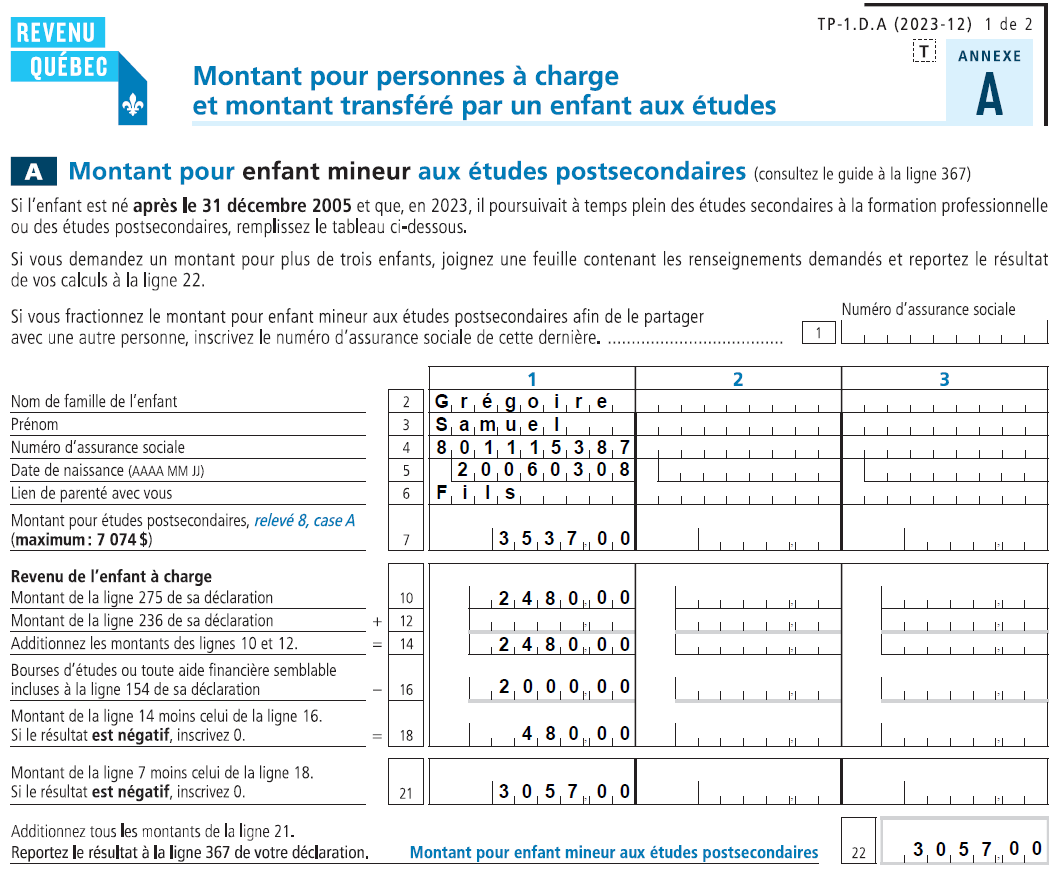
\includegraphics[width=.9\textwidth]{exercice/4-5/Q2/Annexe-A.png}
	\caption[]{Exercice 5, Q2, annexe~A}
	\label{fig:chap4Exercice5Q2AnnexeA}
\end{figure}


\begin{question}
	Michel Soucy est divorcé. Il est propriétaire de sa résidence. Pendant toute l'année, il vivait seul avec sa fille Penelope Soucy, NAS 800 001 216, née le 10 août 2003 (20~ans). Elle a un montant de \numprint{1500}~\$ à la ligne~299 de sa TP1. La case~A de son relevé~8 indique \numprint{7074}~\$. Pour 2023, elle a reçu 305,00~\$ de crédit d'impôt pour solidarité.
\end{question}
\setcounter{sousQuestion}{0}
\begin{sousQuestion}
	Penelope désire transférer à son père le montant pour enfant majeur aux études postsecondaires. Complétez l'\href{https://www.revenuquebec.ca/documents/fr/formulaires/tp/2023-12/TP-1.D.S%282023-12%29.pdf}{annexe~S} de Penelope présentée ci-dessous.
\end{sousQuestion}

Correction: Figure~\ref{fig:chap4Exercice5Q2AnnexeS}.
\begin{figure}
	\centering
	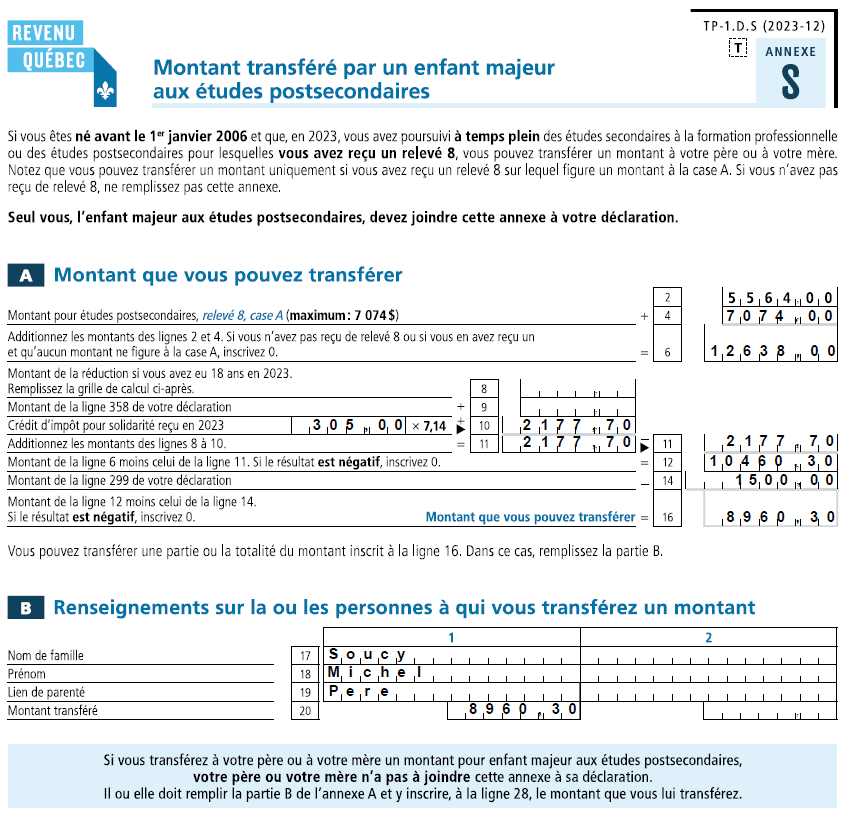
\includegraphics[width=.9\textwidth]{exercice/4-5/Q2/Annexe-S.png}
	\caption[]{Exercice 5, Q2, annexe~S}
	\label{fig:chap4Exercice5Q2AnnexeS}
\end{figure}

\begin{sousQuestion}
	Que doit faire Michel avec le montant que Penelope lui a transféré?
\end{sousQuestion}
Michel doit le reporter aux lignes~28 et 29 de la partie B de son annexe~A.

\begin{sousQuestion}
	Quels sont les documents que Penelope doit joindre à sa TP-1?
\end{sousQuestion}
Elle doit joindre l'annexe~S complétée à sa TP-1. Penelope doit conserver le relevé~8 qu'elle a reçu.

\begin{sousQuestion}
	Est-ce que Michel doit joindre à sa TP-1 l'annexe~S complétée de Penelope et le relevé~8 que Penelope a reçu?
\end{sousQuestion}
Non. Toutefois, il doit joindre l'annexe~A avec la partie B complétée à sa TP-1. Il n'a pas besoin du relevé~8  ni l'annexe~S mais il peut tout de même s'en garder une copie.

\begin{sousQuestion}
	Est-ce que Michel peut réclamer le montant pour personne vivant seule? Expliquez votre réponse.
\end{sousQuestion}
Oui, Michel peut réclamer le montant pour personne vivant seule, parce qu'il a occupé une habitation où il a vécu toute l'année uniquement avec une enfant majeure poursuivant des études postsecondaires à temps plein.

\begin{sousQuestion}
	Nommez trois documents que Michel doit conserver pour justifier sa demande du montant pour personne vivant seule, s'il est admissible.
\end{sousQuestion}
Il devrait avoir en sa possession notamment, soit ses factures de taxes scolaires ou municipales, son bail, son contrat d'assurance habitation, ses factures de téléphone et d'électricité, etc. Il doit conserver ces documents pour justifier sa demande.

\begin{sousQuestion}
	Est-ce que Michel peut réclamer le montant additionnel pour personne vivant seule? Expliquez votre réponse.
\end{sousQuestion}
Oui, Michel peut réclamer le montant additionnel pour personne vivant seule. Il répond aux trois conditions suivantes:
\begin{enumerate}
	\item Il a droit au montant pour personne vivant seule;
	\item Il a vécu avec une enfant majeure qui peut lui transférer un montant pour études postsecondaires;
	\item Il n'a pas recû de paiement de l'allocation famille pour le mois de décembre.
\end{enumerate}

\begin{sousQuestion}
	Michel a inscrit \numprint{42790}~\$ à la ligne~275 de sa déclaration TP-1. Complétez les annexes \href{https://www.revenuquebec.ca/documents/fr/formulaires/tp/2023-12/TP-1.D.A%282023-12%29.pdf}{A} et \href{https://www.revenuquebec.ca/documents/fr/formulaires/tp/2023-12/TP-1.D.B%282023-12%29.pdf}{B} ainsi que la section des crédits d'impôt non remboursables de sa \href{https://www.revenuquebec.ca/documents/fr/formulaires/tp/2023-12/TP-1.D%282023-12%29.pdf}{TP-1}, présentées ci-dessous.
\end{sousQuestion}
Correction:
\begin{itemize}
	\item annexe~A: Figure~\ref{fig:chap4Exercice5Q3AnnexeA}
	\item annexe~B: Figure~\ref{fig:chap4Exercice5Q3AnnexeB}
	\item TP-1: Figure~\ref{fig:chap4Exercice5Q3TP1}
\end{itemize}
\begin{figure}
	\centering
	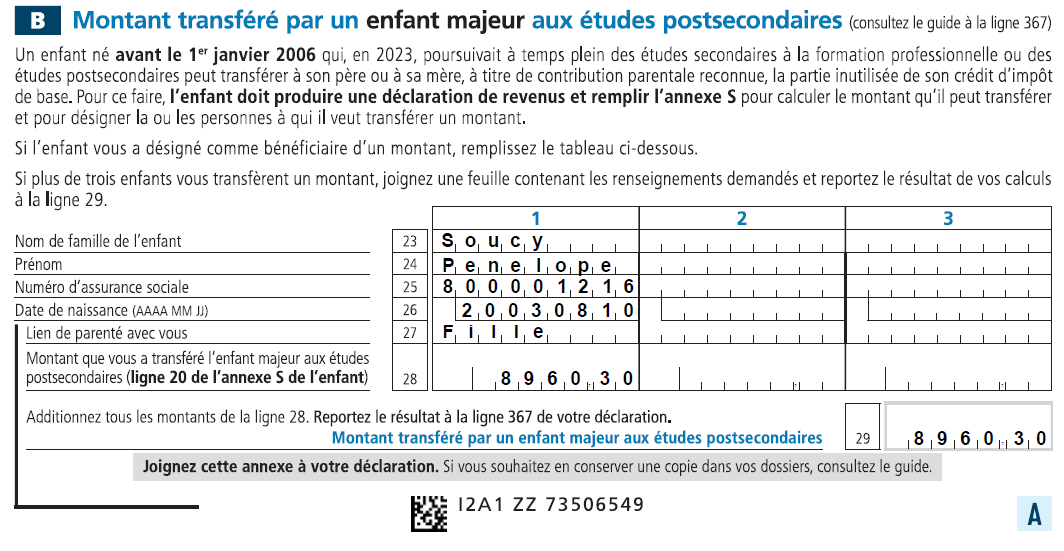
\includegraphics[width=.9\textwidth]{exercice/4-5/Q3/Annexe-A.png}
	\caption[]{Exercice 5, Q3, annexe~A}
	\label{fig:chap4Exercice5Q3AnnexeA}
\end{figure}
\begin{figure}
	\centering
	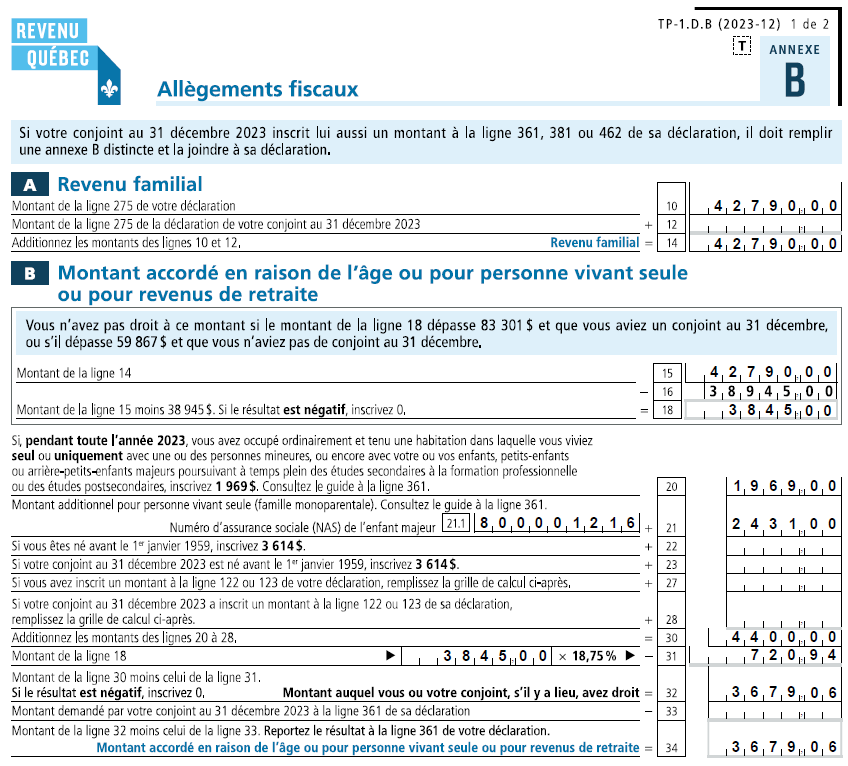
\includegraphics[width=.9\textwidth]{exercice/4-5/Q3/Annexe-B.png}
	\caption[]{Exercice 5, Q3, annexe~B}
	\label{fig:chap4Exercice5Q3AnnexeB}
\end{figure}
\begin{figure}
	\centering
	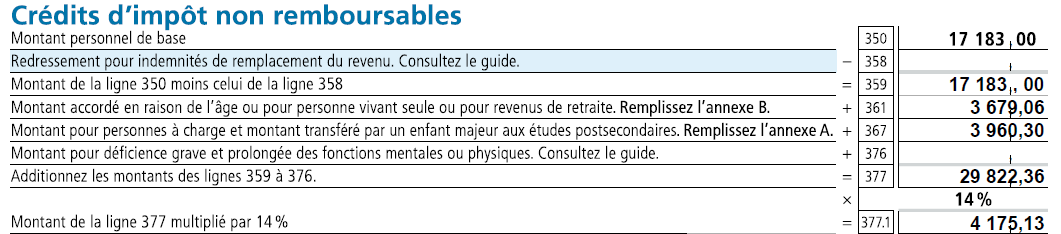
\includegraphics[width=.9\textwidth]{exercice/4-5/Q3/TP-1.png}
	\caption[]{Exercice 5, Q3, TP-1}
	\label{fig:chap4Exercice5Q3TP1}
\end{figure}

\begin{question}
	Supposons que Penelope Soucy, de la question 3, soit née en 2005 (au lieu de 2003) et qu'elle ait eu 18~ans le 10 août 2023. Son relevé~8 indique un montant de \numprint{7074}~\$ à la case~A. Son revenu imposable est de \numprint{1500}~\$ et le revenu net de son père est de \numprint{42790}~\$ sur sa TP-1.
\end{question}
\setcounter{sousQuestion}{0}
\begin{sousQuestion}
	Penelope désire transférer à son père le montant pour enfant majeur aux études postsecondaires. Complétez l'\href{https://www.revenuquebec.ca/documents/fr/formulaires/tp/2023-12/TP-1.D.S%282023-12%29.pdf}{annexe~S} de Penelope.
\end{sousQuestion}
Il y a trois changements par rapport à la question 3:
\begin{itemize}
	\item La grille de calcul \og Montant de la réduction si vous avez eu 18~ans en 2023 \fg{} doit être remplie;
	\item Un montant doit être inscrit à la ligne~8, car Penelope a eu 18~ans en 2023;
	\item Penelope n'a perçu aucun montant du crédit d'impôt pour solidarité en 2023, car elle n'avait pas 18~ans à la fin de l'année d'imposition 2022.
\end{itemize}
annexe~S: Figure~\ref{fig:chap4Exercice5Q4AnnexeS}
\begin{figure}
	\centering
	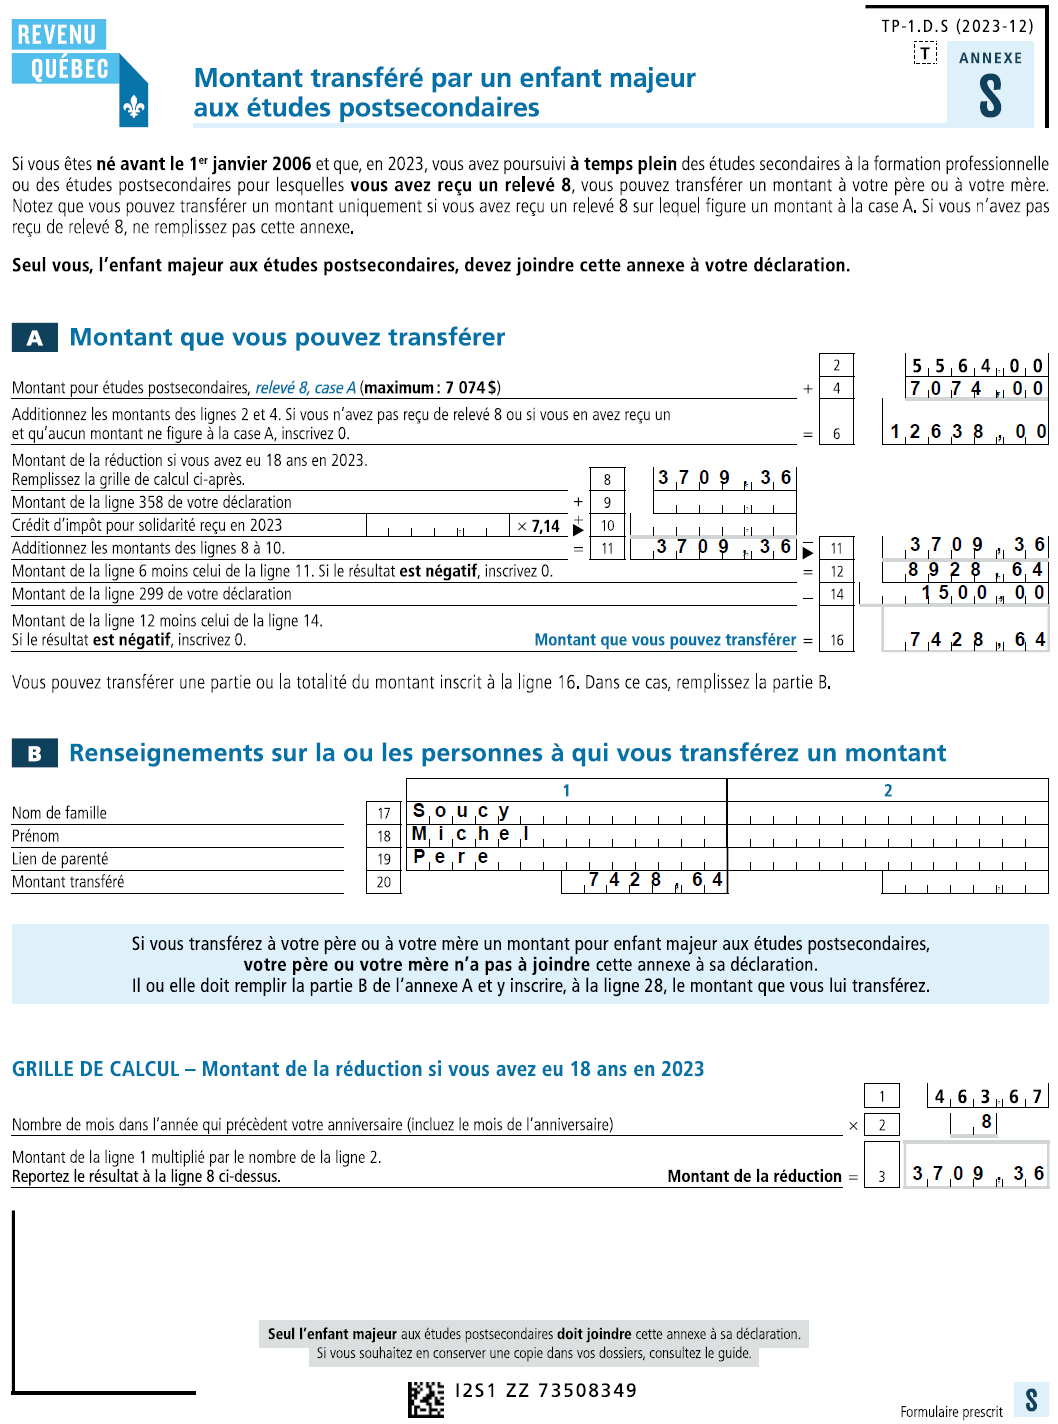
\includegraphics[width=.9\textwidth]{exercice/4-5/Q4/Annexe-S.png}
	\caption[]{Exercice 5, Q4, annexe~S}
	\label{fig:chap4Exercice5Q4AnnexeS}
\end{figure}

\begin{sousQuestion}
	Michel désire réclamer le montant pour personne vivant seule et le montant additionnel pour personne vivant seule. Calculez le montant additionnel pour une personne vivant seule qui peut être demandé.
	
	\rqg{51}
\end{sousQuestion}
Correction: Figure~\ref{fig:chap4Exercice5Q4GrilleCalcul}
\begin{figure}
	\centering
	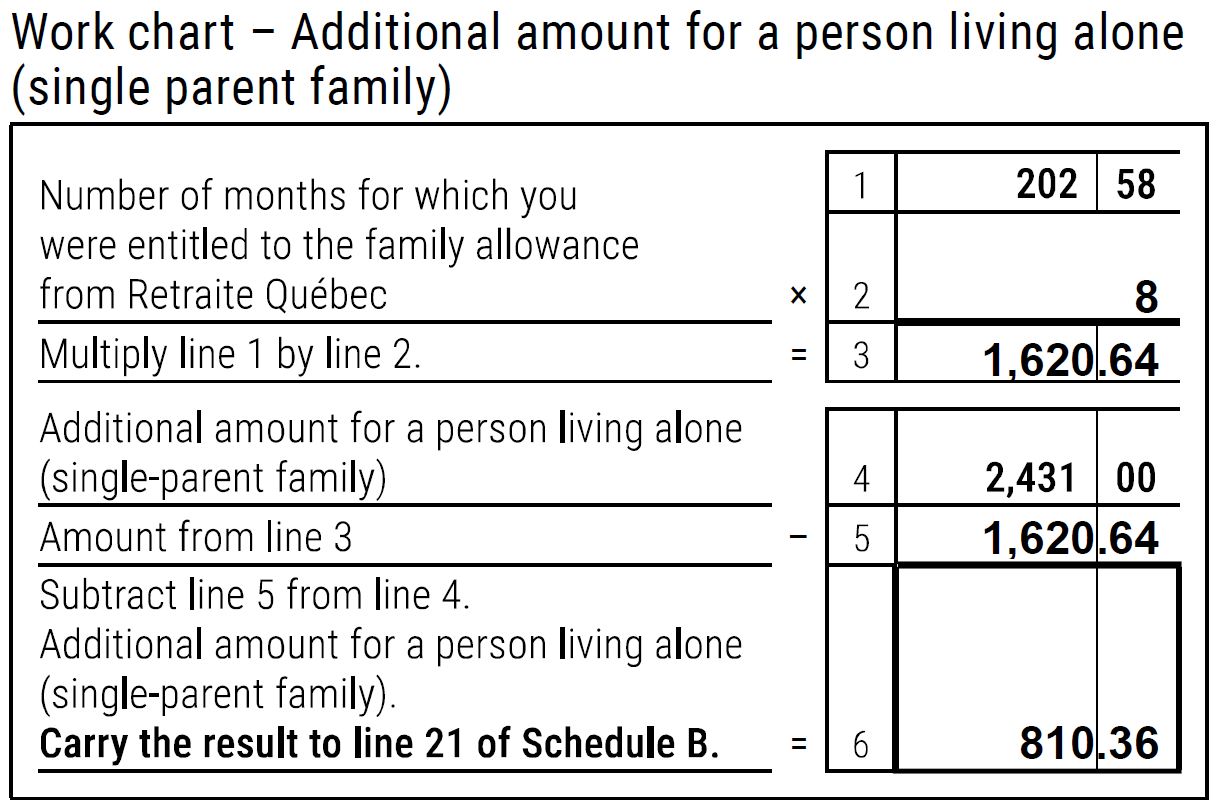
\includegraphics[width=.5\textwidth]{exercice/4-5/Q4/GrilleCalcul.png}
	\caption[]{Exercice 5, Q4, Grille de calcul}
	\label{fig:chap4Exercice5Q4GrilleCalcul}
\end{figure}


\begin{question}
	Pierre Amyot, veuf, dont le NAS est 800 001 232, a vécu avec ses deux fils pendant toute l'année. Il est propriétaire de sa résidence à Laval, Québec:
	
	Benoît, né le 16 août 2007 (16~ans), fréquente l'école secondaire. Il n'avait aucun revenu en 2023.
	Alain est né le 15 juin 2003 (20~ans). Depuis septembre de l'année d'imposition, il étudie à temps plein au Collège de Lévis, au Québec, au niveau postsecondaire. La case~A du relevé~8 qu'il a reçu indique
	\numprint{3537}~\$.
	
\end{question}
\setcounter{sousQuestion}{0}
\begin{sousQuestion}
	Est-ce que Pierre Amyot peut réclamer le montant pour personne vivant seule? Expliquez votre réponse.
\end{sousQuestion}
Oui. Pierre peut réclamer le montant pour personne vivant seule, car il a occupé une habitation dans laquelle il a vécu seul avec une personne mineure et avec un enfant majeur poursuivant à temps plein des études secondaires.

\begin{sousQuestion}
	Est-ce que Pierre Amyot peut réclamer le montant additionnel pour une famille monoparentale? Expliquez votre réponse.
\end{sousQuestion}
Non. Pierre ne peut réclamer le montant additionnel pour personne vivant seule (famille monoparentale), car il a reçu un paiement de l'allocation famille pour son plus jeune enfant.

\begin{sousQuestion}
	Supposons que Alain soit aux études postsecondaires à temps partiel (et non pas à temps plein) et que son relevé~8 n'indique aucun montant à la case~A. Est-ce que Pierre Amyot peut demander le montant pour personne vivant seule? Expliquez votre réponse.
\end{sousQuestion}
Non. Si Alain était aux études à temps partiel, alors Pierre ne répond plus aux conditions pour réclamer le montant pour personne vivant seule, puisqu'il aurait vécu avec un enfant adulte qui ne poursuivait pas des études postsecondaires à temps plein. Par conséquent, Pierre ne pourra pas réclamer le montant additionnel pour personne vivant seule non plus.

\begin{sousQuestion}
	Quel montant Pierre Amyot peut-il demander à l'égard de Benoît sur sa déclaration du Québec? Expliquez votre réponse.
\end{sousQuestion}
Pierre ne peut réclamer aucun montant pour Benoît sur sa déclaration provinciale.

Au Québec, les paiements de l'allocation famille versés par le gouvernement québécois remplacent les montants pour enfants mineurs. Il serait possible de réclamer un montant pour enfant mineur seulement si ce dernier est aux études postsecondaires à temps plein. Ce n'est pas le cas de Benoît.

\begin{sousQuestion}
	Quel montant Pierre Amyot peut-il demander à l'égard de ses deux enfants sur sa déclaration fédérale? Expliquez votre réponse.
\end{sousQuestion}
Pierre peut réclamer le montant pour personne à charge admissible à l'égard de Benoît à la ligne~30400 de sa T1.

Au fédéral, Pierre ne peut réclamer aucun montant pour Alain qui a plus de 18~ans. Il serait possible de réclamer un montant pour enfant majeur seulement s'il est déficient.



\section{Crédits d'impôt non remboursables au Québec}
\begin{intro}
	Nous venons de terminer une partie importante des crédits d'impôt concernant le Québec. Comme vous l'avez vu, le contribuable ou ses personnes à charge peuvent avoir à remplir des annexes justificatives pour déterminer les crédits à réclamer sur sa déclaration TP-1.
\end{intro}

\begin{note}
	Le montant de la ligne~378 (frais pour soins médicaux non dispensés dans votre région), de la ligne~381 (frais médicaux) et la 385 (intérêts payés sur un prêt étudiant) correspond à un crédit d'impôt non remboursable de 20~\%. Ces crédits seront discutés plus loin dans le cours.
\end{note}

\begin{note}
	Entre les lignes~378 à 385 et les lignes~389 à 398.1, il y a des crédits non-remboursables supplémentaires qui sont à des taux différents de 14~\%. Ces montants seront abordés dans les chapitres suivants.
\end{note}



\section{Sommaire du chapitre}

\begin{itemize}[label=\twemoji{star}]
	\item La définition d'une personne à charge.
	\item Au fédéral:
	\begin{itemize}
		\item Le montant personnel de base.
		\item Le montant pour époux ou conjoint de fait.
		\item Le montant pour une personne à charge admissible.
		\item Le montant canadien pour aidant naturel pour époux ou conjoint de fait ou pour une personne à charge admissible âgée de 18~ans ou plus.
		\item Le montant canadien pour aidant naturel pour autres personnes à charge âgées de 18~ans ou plus ayant une déficience.
		\item Le montant canadien pour aidant naturel pour enfants âgés de moins de 18~ans ayant une déficience.
		\item Le crédit TPS.
		\item L'allocation canadienne pour enfants.
	\end{itemize}
	\item Au Québec:
	\begin{itemize}
		\item Le montant personnel de base.
		\item Montant accordé à une personne vivant seule.
		\item Montant additionnel pour personne vivant seule (famille monoparentale).
		\item Montant pour enfant mineur aux études postsecondaires.
		\item Montant transféré par un enfant majeur aux études postsecondaires.
		\item Montant pour autres personnes à charge.
		\item Le crédit pour solidarité.
		\item L'allocation familiale pour enfants.
	\end{itemize}
\end{itemize}



\section{Problème de révision}
Ce couple a deux enfants et un autre adulte à charge. Le couple sait qu'il peut réclamer plusieurs crédits d'impôt, mais il ne sait pas par où commencer. Ils ont besoin de votre aide pour demander le nombre maximum de crédits qu'ils peuvent obtenir.


\subsection{Renseignements des contribuables}
Voir la table \ref{table:chapitre4ProblemeRenseignementsContribuables}.
\begin{table}
	\centering
	\begin{tabular}{|l|c|c|}
		\hline
		\rowcolor{LightGreen} Description        & Contribuable 1 &        Contribuable 2        \\ \hline
		Nom                                      & Daniel Hébert  &          Catherine           \\
		                                         &                &           Gauthier           \\ \hline
		NAS                                      &  801 115 411   &         801 115 429          \\ \hline
		Date de naissance                        &  22 mars 1980  &       1\ier{} mai 1982       \\ \hline
		Statut civil                             &          \multicolumn{2}{c|}{Mariés}          \\ \hline
		Sexe                                     &       M        &              F               \\ \hline
		Province de résidence                    &       QC       &              QC              \\ \hline
		Langue                                   &       A        &              F               \\ \hline
		Téléphone                                &  514-362-9109  &           Le même            \\ \hline
		Adresse courriel 1                       &      \multicolumn{2}{c|}{dhebert@bnc.ca}      \\ \hline
		Adresse courriel 2                       &   \multicolumn{2}{c|}{cgauthier@laforme.ca}   \\ \hline
		Consentement à l'envoi de communications &      Oui       &             Oui              \\
		par voie électronique uniquement         &                &                              \\ \hline
		Régime d'assurance médicaments           &     Privé      &            Privé             \\ \hline
		Adresse                                  & \multicolumn{2}{c|}{10 rue Bordeaux, App. 4,} \\
		                                         &  \multicolumn{2}{c|}{Montréal, QC, H3R 5Y9}   \\ \hline
		Citoyenneté canadienne                   &      Oui       &             Oui              \\ \hline
		Élections Canada                         &      Oui       &             Oui              \\ \hline
		Biens étrangers                          &      Non       &             Non              \\ \hline
		Revenu                                   &      Oui       &             Oui              \\ \hline
	\end{tabular}
	\caption[]{Problème, renseignements des contribuables}
	\label{table:chapitre4ProblemeRenseignementsContribuables}
\end{table}


\subsection{Renseignements sur les personnes à charge}
Voir la table \ref{table:chapitre4ProblemeRenseignementsPersonnesACharge}.
\begin{table}
	\centering
	\begin{tabular}{|l|c|c|c|}
		\hline
		\rowcolor{LightGreen} Description &    Personne     &    Personne     &    Personne     \\
		\rowcolor{LightGreen}             &   à charge 1    &   à charge 2    &   à charge 3    \\ \hline
		Nom                               & Sylvain Hébert  & Yannick Hébert  &  Éva Gauvreau   \\ \hline
		Lien                              &      Fils       &      Fils       & Tante de Daniel \\ \hline
		NAS                               &      S. O.      &   801-115-437   &   801 115 445   \\ \hline
		Date de naissance                 & 22 octobre 2010 & 16 juillet 2005 & 22 février 1959 \\ \hline
	\end{tabular}
	\caption[]{Problème, renseignements sur les personnes à charge}
	\label{table:chapitre4ProblemeRenseignementsPersonnesACharge}
\end{table}


\subsection{Informations supplémentaires du couple}
\begin{itemize}
	\item Daniel est technicien en informatique pour la Banque Nationale du Canada.
	\item Catherine travaille au service à la clientèle de la société La Forme.
	\item Le couple est locataire du logement et chacun possède son RL-31.
	\item Le couple a reçu l'allocation canadienne pour enfant.
	\item Catherine veut demander le crédit d'impôt pour solidarité.
\end{itemize}


\subsection{Informations supplémentaires pour les personnes à charge}
\begin{enumerate}
	\item Sylvain n'a eu aucun revenu en 2023.
	\item Yannick poursuit des études postsecondaires au Collège de Montréal. Il a complété une session et a reçu un relevé~8.
	\begin{enumerate}
		\item En 2023, il a gagné \numprint{1980}~\$ d'un travail à temps partiel à la Ville de Montréal. Il a contribué les montants suivants:
		\begin{enumerate}
			\item 25,15~\$ à l'Assurance-emploi (AE);
			\item 0,00~\$ à la Régie des rentes du Québec (RRQ);
			\item 9,78~\$ au Régime québécois d'assurance parentale (RQAP).
		\end{enumerate}
		\item Au fédéral, le revenu net de Yannick est de \numprint{1980}~\$.
		\item Au Québec, son revenu net et son revenu imposable est de \numprint{1861,20}~\$.
		\item Yannick accepte de transférer à son père le montant pour études postsecondaires.
		\item Il n'a pas reçu de crédit de solidarité en 2023, car il a eu 18~ans en 2023.
	\end{enumerate}
	\item Éva vit avec Daniel et Catherine depuis 3~ans.
	\begin{enumerate}
		\item Elle souffre d'une déficience physique attestée par son médecin, depuis 4~ans.
		\item Le revenu net de Éva est de \numprint{14450}~\$ au fédéral et au Québec.
		\item Utilise l'assurance médicaments du Québec toute l'année.
	\end{enumerate}
\end{enumerate}

La déduction pour la bonification au RRQ est de 436,00~\$ pour Daniel et de 51,25~\$ pour Catherine.


\subsection{Feuillets}
\begin{center}
	\begin{tabular}{|c|c|c|c|}
		\hline
		&
			Daniel &
			Catherine & 
			Yannick \\ \hline
		RL-31 &
			Figure~\ref{fig:chap4ProblemeDanielRL31} &
			Figure~\ref{fig:chap4ProblemeCatherineRL31} &
			\\ \hline
		T4 &
			Figure~\ref{fig:chap4ProblemeDanielT4} &
			Figure~\ref{fig:chap4ProblemeCatherineT4} &
			\\ \hline
		RL-1 &
			Figure~\ref{fig:chap4ProblemeDanielRL1} &
			Figure~\ref{fig:chap4ProblemeCatherineRL1} &
			\\ \hline
		RL-8 &
			&
			&
			Figure~\ref{fig:chap4ProblemeYannickRL8} \\ \hline
	\end{tabular}
\end{center}

\begin{figure}
	\centering
	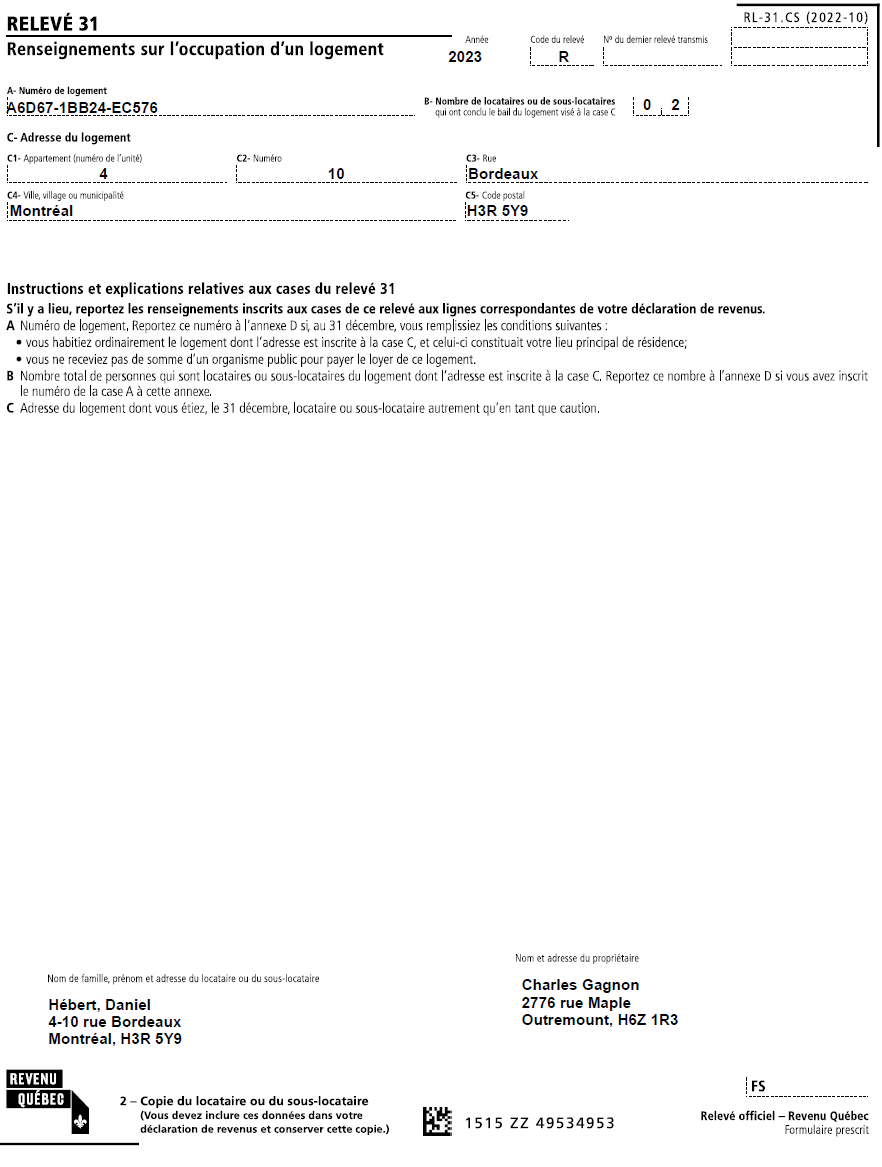
\includegraphics[width=.9\textwidth]{probleme/chapitre-4/Daniel-RL31.png}
	\caption[]{Problème, RL-31 de Daniel}
	\label{fig:chap4ProblemeDanielRL31}
\end{figure}
\begin{figure}
	\centering
	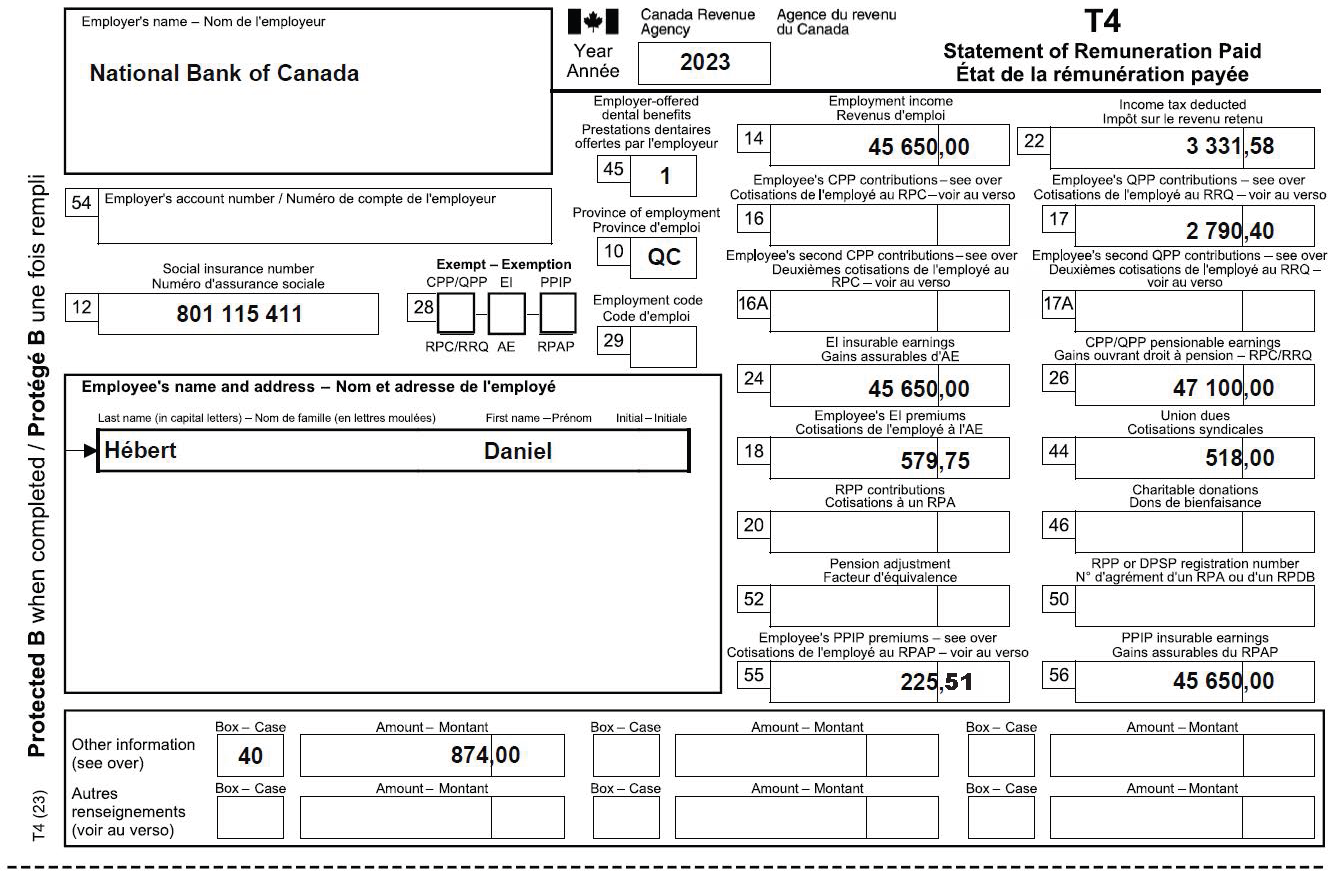
\includegraphics[width=.9\textwidth]{probleme/chapitre-4/Daniel-T4.png}
	\caption[]{Problème, T4 de Daniel}
	\label{fig:chap4ProblemeDanielT4}
\end{figure}
\begin{figure}
	\centering
	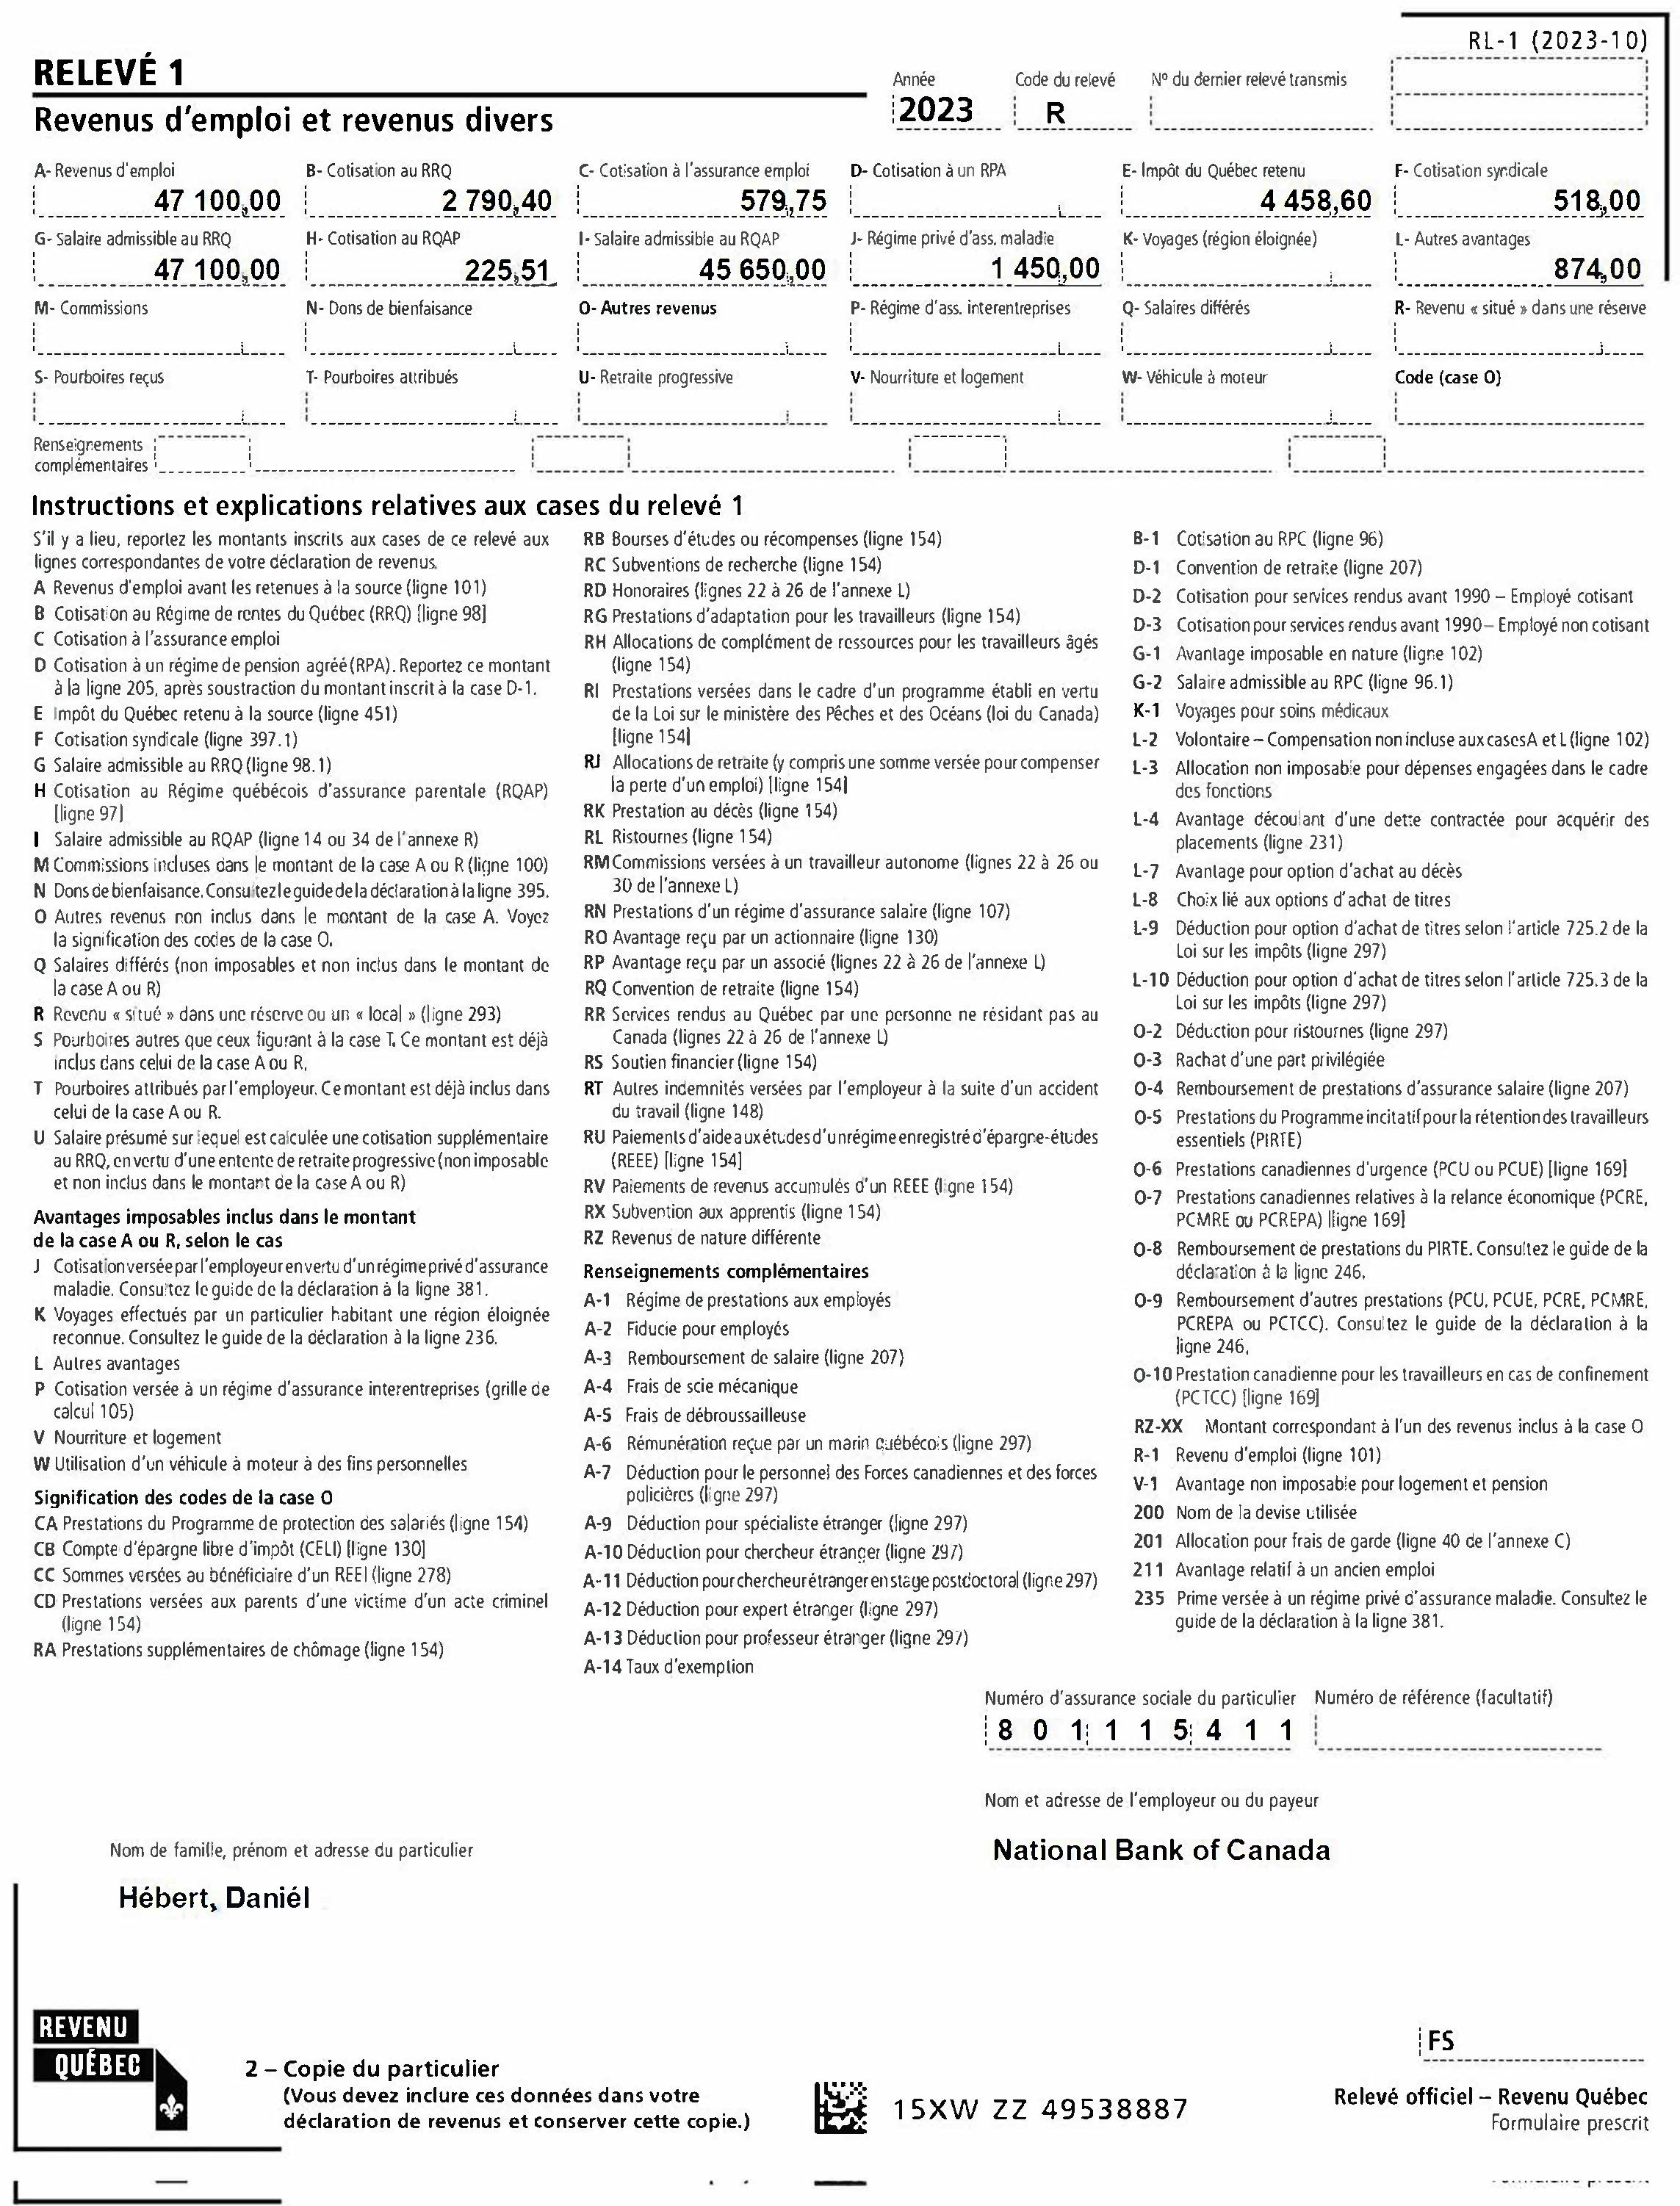
\includegraphics[width=.9\textwidth]{probleme/chapitre-4/Daniel-RL1.png}
	\caption[]{Problème, RL-1 de Daniel}
	\label{fig:chap4ProblemeDanielRL1}
\end{figure}
\begin{figure}
	\centering
	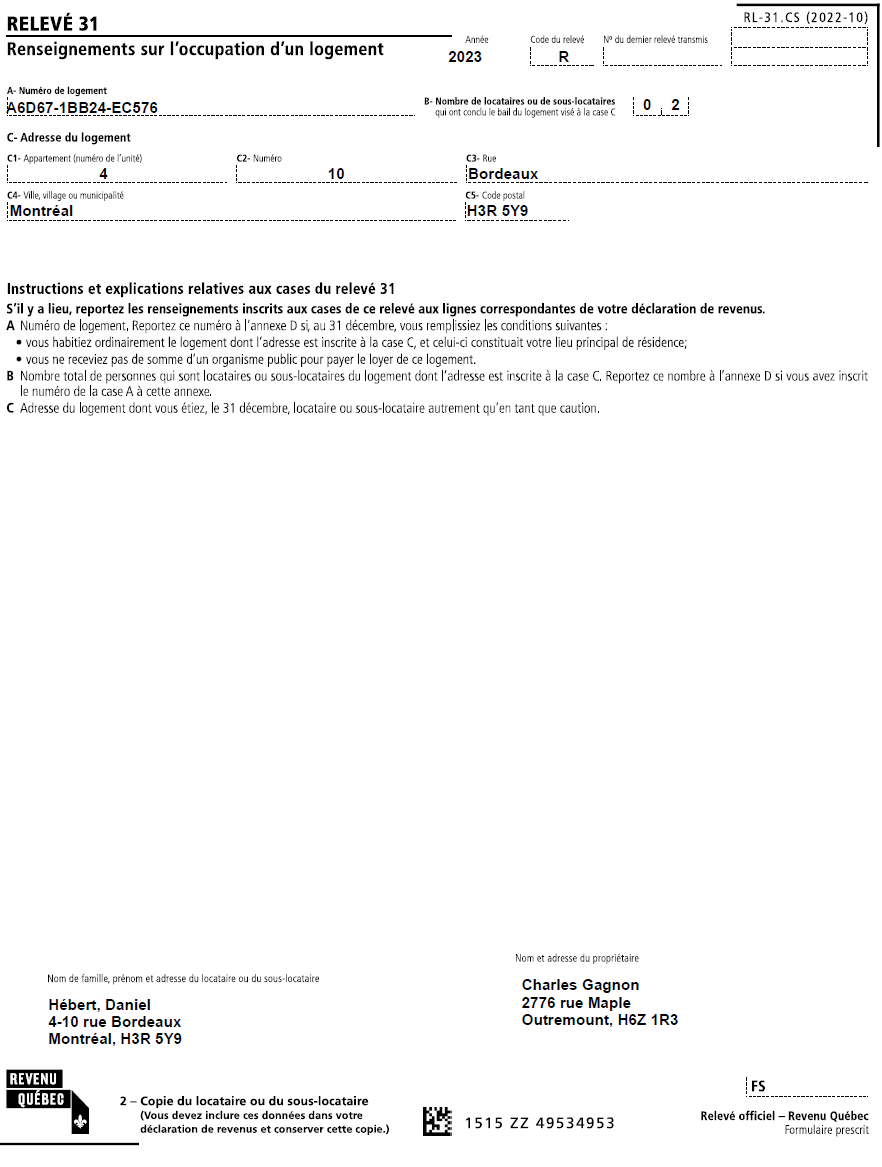
\includegraphics[width=.9\textwidth]{probleme/chapitre-4/Daniel-RL31.png}
	\caption[]{Problème, RL-31 de Catherine}
	\label{fig:chap4ProblemeCatherineRL31}
\end{figure}
\begin{figure}
	\centering
	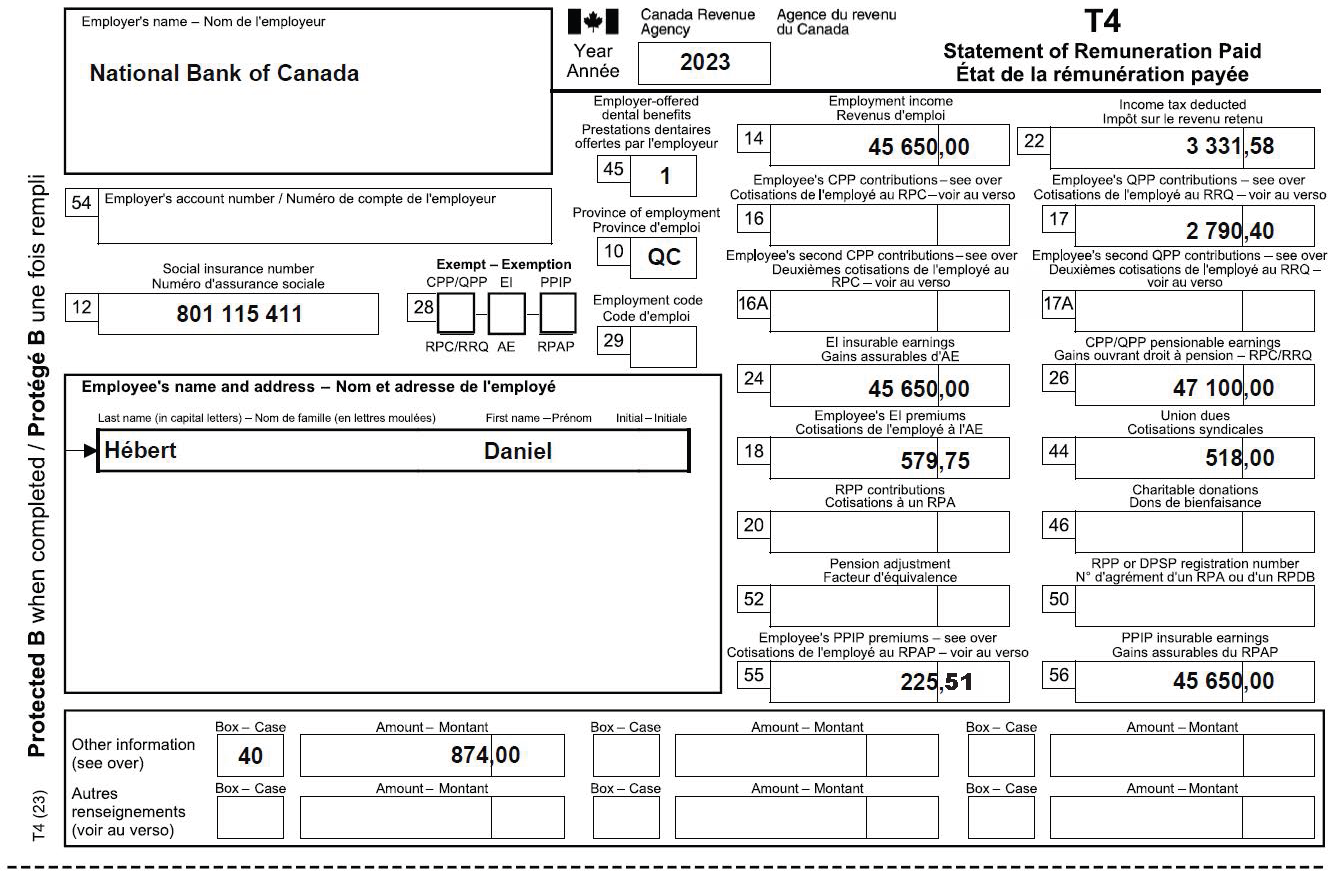
\includegraphics[width=.9\textwidth]{probleme/chapitre-4/Daniel-T4.png}
	\caption[]{Problème, T4 de Catherine}
	\label{fig:chap4ProblemeCatherineT4}
\end{figure}
\begin{figure}
	\centering
	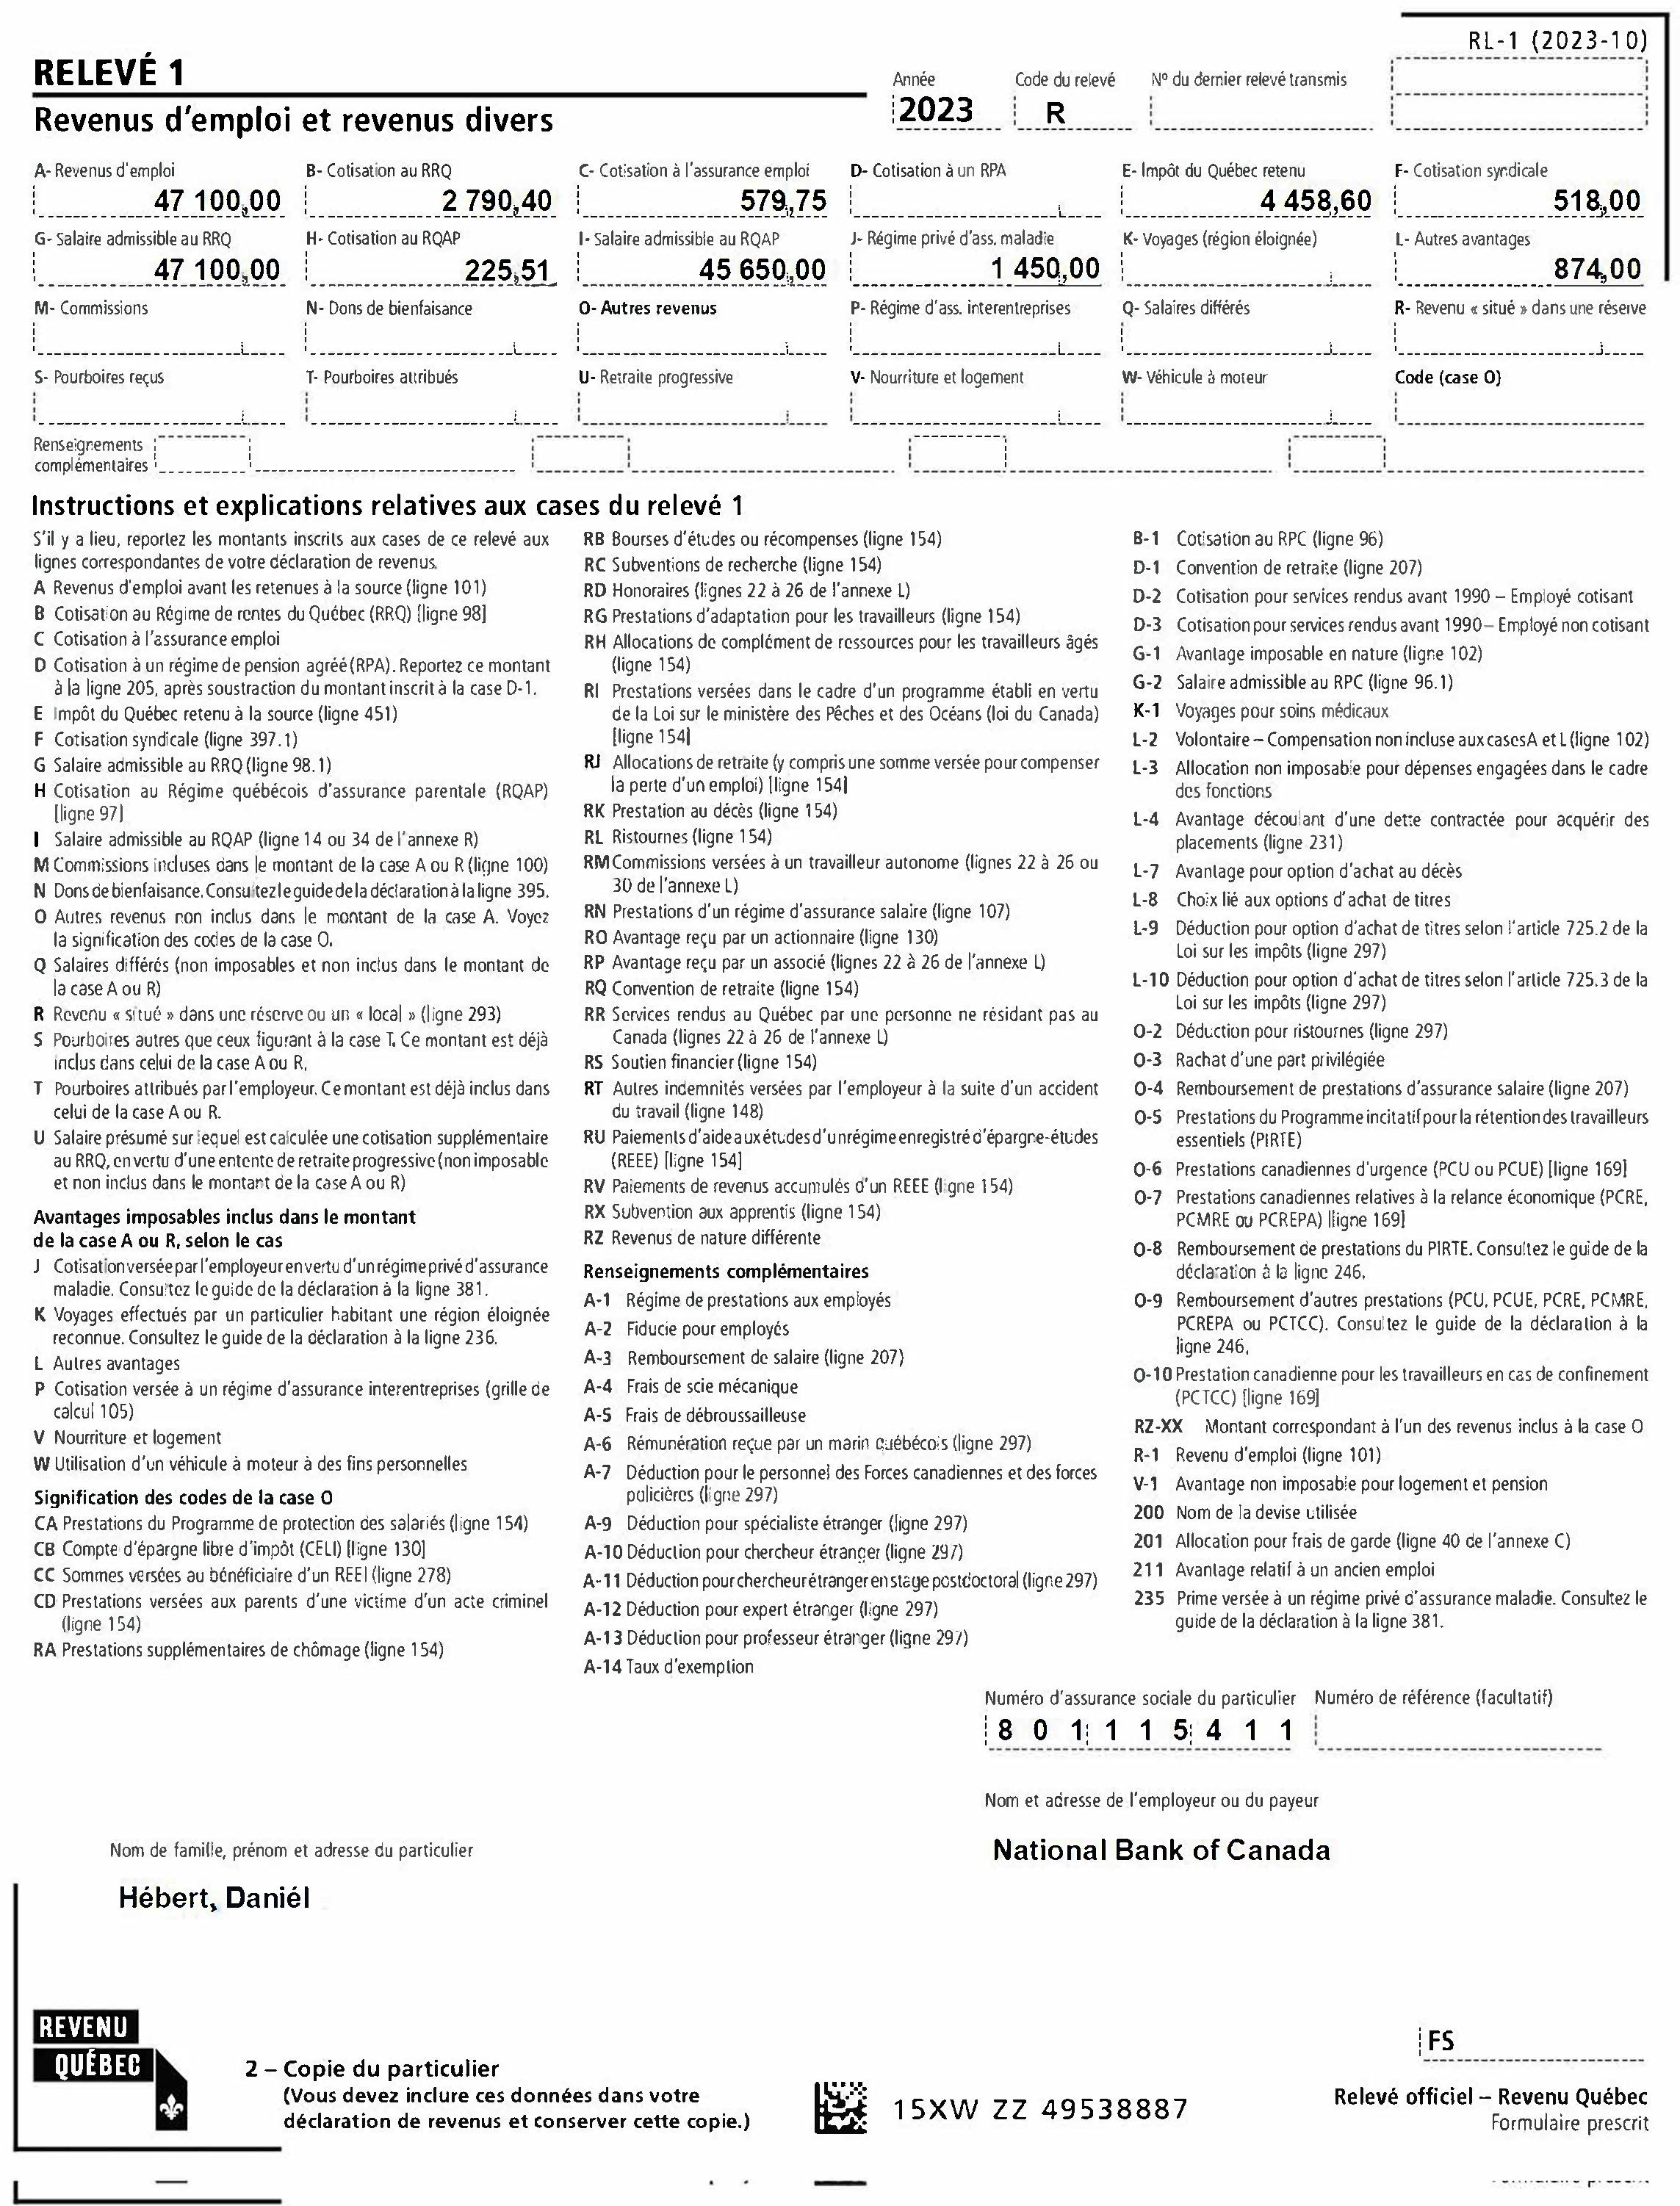
\includegraphics[width=.9\textwidth]{probleme/chapitre-4/Daniel-RL1.png}
	\caption[]{Problème, RL-1 de Catherine}
	\label{fig:chap4ProblemeCatherineRL1}
\end{figure}
\begin{figure}
	\centering
	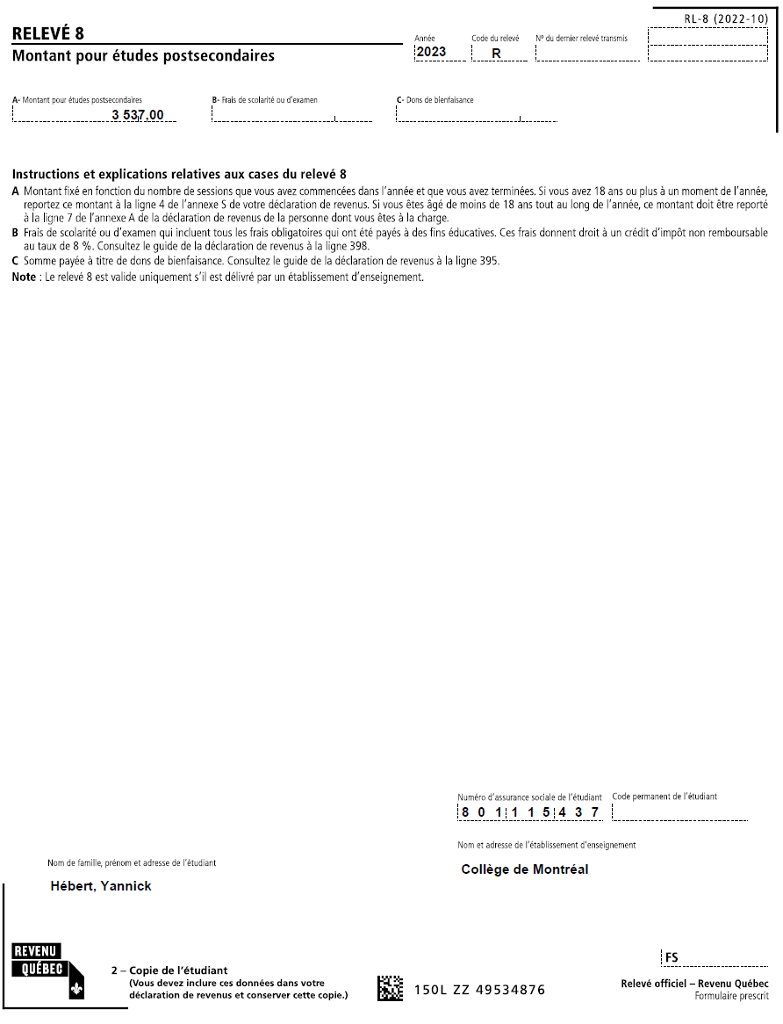
\includegraphics[width=.9\textwidth]{probleme/chapitre-4/Yannick-RL8.png}
	\caption[]{Problème, RL-8 de Yannick}
	\label{fig:chap4ProblemeYannickRL8}
\end{figure}


\subsection{Instructions}
\begin{enumerate}
	\item À l'aide des renseignements fournis, remplissez les étapes 2, 3, 4 et l'étape 5 de la partie B des déclarations \href{https://www.canada.ca/fr/agence-revenu/services/formulaires-publications/trousses-impot-toutes-annees-imposition/trousse-generale-impot-prestations/quebec/5005-r.html}{T1} de Daniel et Catherine, en utilisant l'\href{https://www.canada.ca/fr/agence-revenu/services/formulaires-publications/trousses-impot-toutes-annees-imposition/trousse-generale-impot-prestations/5000-s5.html}{annexe~5} pour calculer les montants des lignes~30300 et 30450.
	\item Remplissez l'\href{https://www.revenuquebec.ca/documents/fr/formulaires/tp/2023-12/TP-1.D.S%282023-12%29.pdf}{annexe~S} de Yannick.
	\item Remplissez la déclaration \href{https://www.revenuquebec.ca/documents/fr/formulaires/tp/2023-12/TP-1.D%282023-12%29.pdf}{TP-1} de Daniel et Catherine (arrêtez-vous lorsque vous atteignez la partie Impôt sur le revenu et cotisations), ainsi que leurs annexes \href{https://www.revenuquebec.ca/documents/fr/formulaires/tp/2023-12/TP-1.D.A%282023-12%29.pdf}{A} et \href{https://www.revenuquebec.ca/documents/fr/formulaires/tp/2023-12/TP-1.D.D%282023-12%29.pdf}{D}.
\end{enumerate}



\section{Autotest \no 2}
\setcounter{question}{0}
\begin{question}
	Martine a hébergé sa meilleure amie durant toute l'année d'imposition. Son amie a eu un revenu net de \numprint{12000}~\$ en 2023. Quel montant Martine peut-elle demander pour son amie en tant que personne à charge admissible, étant donné que son propre montant personnel de base est de \numprint{15000}~\$?
	\begin{enumerate}
		\item 	\numprint{6000}~\$, soit 50~\% de \numprint{12000}~\$
		\item 	0,00~\$, elle ne peut pas réclamer le crédit
		\item 	\numprint{3000}~\$, soit \numprint{15000}~\$ - \numprint{12000}~\$
		\item 	\numprint{2499}~\$ comme montant pour aidant naturel
	\end{enumerate}
\end{question}
0,00~\$, elle ne peut pas réclamer le crédit.

Sa meilleure amie ne peut pas être considérée comme une personne à charge admissible. Rien ne peut donc être réclamé.

\begin{question}
	Jean-Paul, âgé de 74 ans, a vécu avec son fils François et la conjointe de François au cours de l'année d'imposition. Jean-Paul a un revenu net de \numprint{20000}~\$. Quel montant de crédit à la ligne~30450 de la déclaration fédérale François ou son épouse peuvent-ils demander pour Jean-Paul?
	\begin{enumerate}[label=\Alph*.]
		\item \numprint{6782}~\$, soit \numprint{26782}~\$ - \numprint{20000}~\$ 
		\item \numprint{7999}~\$
		\item \numprint{2499}~\$ comme montant pour aidant naturel
		\item 0~\$, aucun des deux ne peut réclamer un montant pour Jean-Paul
	\end{enumerate}
\end{question}
0~\$, aucun des deux ne peut réclamer un montant pour Jean-Paul.

Comme on ne nous dit pas si Jean-Paul est infirme, alors aucun montant ne pourra être réclamé. Si Jean-Paul était infirme, ils pourraient alors réclamer \numprint{6782}~\$.

\begin{question}
	Gaston et Nancy sont des conjoints de fait. Gaston a un revenu net de \numprint{9159}~\$ et est atteint d'une infirmité. Nancy aimerait demander le montant pour époux ou conjoint de fait. Si Nancy a un revenu net de \numprint{240000}~\$, quel montant peut-elle réclamer?
	\begin{enumerate}[label=\Alph*.]
		\item \numprint{4361,00}~\$
		\item \numprint{5841,25}~\$
		\item \numprint{6860,00}~\$
		\item \numprint{8340,75}~\$
	\end{enumerate}
\end{question}
\numprint{6860,00}~\$

(\numprint{13520}~\$ + \numprint{2499}~\$ - \numprint{9159}~\$)

\begin{question}
	Johanne est chef de famille monoparentale et vit seule avec son fils âgé de 8~ans. Quel montant (\$) peut-elle demander pour son fils et sur quelle ligne de sa T1 si son revenu net est de \numprint{165430}~\$?
	\begin{enumerate}[label=\Alph*.]
		\item \numprint{15000}~\$ à la ligne~30400
		\item \numprint{15000}~\$ à la ligne~30500
		\item \numprint{13520}~\$ à la ligne~30400
		\item \numprint{13520}~\$ à la ligne~30500
	\end{enumerate}
\end{question}
\numprint{15000}~\$ à la ligne~30400

(\numprint{165430}~\$ est la limite pour le maximum de \numprint{15000}~\$)

\begin{question}
	Karine est une mère célibataire qui vit seule avec sa fille âgée de 17~ans. Quel montant peut-elle demander pour une personne vivant seule dans sa déclaration TP-1 si son revenu net est de \numprint{38900}~\$?
	\begin{enumerate}[label=\Alph*.]
		\item \numprint{4400}~\$
		\item \numprint{3614}~\$
		\item \numprint{2431}~\$
		\item \numprint{1969}~\$
	\end{enumerate}
\end{question}
\numprint{1969}~\$ (annexe B, ligne 20)
% Montants personnels
\chapter{Calcul des impôts et crédits}% Calcul des impôts et crédits
%\chapter{Revenus de placement}% Revenus de placement
%\chapter{Prestations sociales}
\section{Introduction et objectifs}
\subsection{Introduction}
Dans ce chapitre, nous discutons de plusieurs prestations sociales que les contribuables peuvent recevoir et de la manière dont ils sont traités comme un revenu dans les déclarations de revenus. Nous discutons également des prestations reçues du Régime de rentes du Québec, de l'assurance-emploi fédérale et de l'assurance parentale du Québec. Certaines prestations peuvent devoir être remboursées et nous discutons du traitement fiscal de ces remboursements. Enfin, nous étudions le traitement fiscal des frais juridiques , des dons de bienfaisance et de deux principaux crédits d'impôt remboursables disponibles pour les revenus d'emploi faibles à modestes.


\subsection{Objectifs}
\begin{itemize}[label=\twemoji{check mark button}]
	\item Expliquer le Programme de protection des salariés et déclarer les sommes reçues;
	\item Déclarer les indemnités pour les accidents du travail, pour les accidentés de la route et pour les victimes d'acte criminel;
	\item Déclarer les prestations d'assistance sociale, et toute aide financière semblable;
	\item Déclarer les sommes reçues du Régime de rentes du Québec;
	\item Déclarer les prestations d'assurance-emploi;
	\item Déterminer le montant du remboursement des prestations d'assurance-emploi et le traiter;
	\item Déclarer les prestations versées par le gouvernement fédéral et Québec à cause de la COVID-19;
	\item Déclarer les prestations d'assurance parentale;
	\item Déclarer les \og Autres revenus \fg{} et \og Autres montants \fg{};
	\item Identifier les frais juridiques que le contribuable peut déduire;
	\item Réclamer les \og Autres déductions \fg{};
	\item Réclamer le montant pour l'achat d'une habitation au fédéral et Québec;
	\item Identifier les dons qui sont considérés comme des dons de bienfaisance, et calculer le crédit d'impôt non remboursable relatif à ces dons;
	\item Aux fins de l'impôt du Québec, expliquer en quoi consiste le crédit pour la prime au travail, le crédit pour la prime au travail adaptée et le crédit pour le supplément à la prime au travail, et les réclamer;
	\item Aux fins de l'impôt fédéral, expliquer en quoi consiste le crédit d'impôt pour allocation canadienne pour les travailleurs, et le réclamer;
	\item Expliquer les conditions à remplir pour bénéficier de crédit d'impôt Bouclier fiscal, et le réclamer;
	\item Expliquer en quoi consiste le crédit d'impôt pour mise aux normes d'installations d'assainissement des eaux usées résidentielles offert par le gouvernement du Québec, et le réclamer.
\end{itemize}


\subsection{Sujets du chapitre}
\begin{itemize}
	\item CNESST
	\item Prestations RRQ, RQAP, et AE
	\item Achat habitation
	\item Bouclier fiscal
	\item Aide financière aux familles
	\item Dons
	\item ACT et Prime au travail
\end{itemize}



\section{T5007 et Relevé~5}
\begin{intro}
	Dans les prochaines parties, nous allons discuter de plusieurs prestations sociales qui sont inscrites sur le T5007 et le Relevé~5.
	
	Vous remarquerez que le Québec accorde des indemnités qui ne sont pas inscrites comme revenu sur le feuillet fédéral. Ces indemnités sont exonérées d'impôt sur la T1.
\end{intro}


\subsection{T5007}
Le feuillet fiscal \href{https://www.canada.ca/fr/agence-revenu/services/formulaires-publications/formulaires/t5007.html}{T5007} est émis pour enregistrer les paiements pour les prestations fédérales suivantes:
\begin{itemize}
	\item Indemnité pour accidents du travail;
	\item Prestation d'assistance sociale.
\end{itemize}


\subsection{Relevé~5}
Le \href{https://www.revenuquebec.ca/fr/services-en-ligne/formulaires-et-publications/details-courant/rl-5/}{Relevé~5} est émis pour enregistrer les versements des prestations et indemnités suivantes versées par le Québec: 
\begin{itemize}
	\item CNESST
	\item Assistance sociale
	\item Aide financière gouvernementale
	\item Indemnités de la SAAQ
	\item Indemnités pour actes de civisme, victimes d'actes criminels, arrêt préventif d'activité et aide au remplacement du revenu.
\end{itemize}



\section{Accidents du travail}
\begin{intro}
	L'indemnisation des victimes d'accident du travail est une sorte d'assurance qui vise à compenser les difficultés occasionnées par une maladie, un accident ou un décès liés au travail. Le programme, financé par des cotisations patronales basées sur la masse salariale, est utilisé pour couvrir les coûts des soins médicaux et de la réadaptation des travailleurs.
\end{intro}

\index{Travailleur}
Dans ce contexte, un \og travailleur \fg{} est une personne qui exerce un travail rémunéré pour un employeur en vertu d'un contrat de travail.

Dans les provinces et territoires du Canada, il existe des lois qui établissent les droits et les obligations des travailleurs et des employeurs lorsqu'il y a une maladie, un accident ou un décès relié au travail. Au Québec, on retrouve la \acrfull{lsst}, qui traite de la prévention et de l'inspection, et la \acrfull{latmp}, qui régit l'indemnisation et la réadaptation des travailleurs.

En général, ces lois confient aux employeurs et aux travailleurs la responsabilité de la santé et de la sécurité au travail dans leur milieu de travail. La \acrfull{cnesst} est chargée de leur application. 


\subsection{Qui verse les indemnités pour un accident du travail?}
Les indemnités pour un accident du travail sont versées par la CNESST. Cet organisme remet un feuillet~T5007 et un relevé~5 aux personnes qui ont reçu des indemnités durant l'année d'imposition.

Les prestations versées par la CNESST sont indiquées à la case~10 du feuillet~T5007 et à la case~C du Relevé~5. Ces prestations ne sont \textbf{pas imposables}; cependant, ils doivent être inclus dans le revenu total et le revenu net avant d'être déduits avant le revenu imposable.

\subsection{Attente d'une décision de la CNESST}
En attendant la décision de la CNESST, l'employeur peut continuer à verser des sommes à l'employé. Ces montants sont déclarés selon la nature du revenu:
\begin{itemize}
	\item Si l'employeur lui verse un salaire, le montant constitue un revenu d'emploi et sera déclaré sur des T4 et relevé~1;
	\item S'il lui verse une avance sur indemnités, aucun montant ne doit être déclaré parce que cette somme sera remboursée par la CNESST à l'employeur lorsque la demande sera approuvée;
	\item S'il lui verse un prêt, aucun montant ne doit être déclaré;
	\item S'il lui verse des prestations d'assurance salaire provenant d'un régime collectif d'assurance salaire, l'imposition de ce revenu dépend de la personne qui a versé les cotisations au régime et du degré de contrôle exercé par l'employeur sur le régime. Si nécessaire, revoir la discussion sur ce sujet au chapitre 2.
\end{itemize}

\subsubsection{Remboursement des sommes versées par l'employeur}
Lorsque la CNESST reconnaît que l'employé a droit à une indemnité, les sommes versées par l'employeur durant la période d'attente d'une décision de la CNESST lui sont remboursées. Elles constituent des indemnités de remplacement du revenu et l'employé recevra un feuillet~T5007 et un relevé~5. 

Il arrive que la demande soumise à la CNESST soit approuvée dans une année subséquente. Par exemple, si une demande déposée en 2022 est approuvée en 2023, l'employé peut avoir déclaré les sommes versées par l'employeur à titre de revenus imposables en 2022. En 2023, lorsque la demande est approuvée, l'employeur reçoit un remboursement de la CNESST. L'employeur émettra les feuillets suivants:

\begin{itemize}[label=\twemoji{check box with check}]
	\item Un T4 avec le montant du remboursement à la case~77:
	\begin{itemize}
		\item Le contribuable pourra réclamer une déduction correspondant au remboursement à la ligne~22900 de sa T1;
	\end{itemize}
	\item Un relevé~1 avec le montant du remboursement:
	\begin{itemize}
		\item À la case~A-3;
		\item À la case~O-4, si la somme versée par l'employeur a été déclarée à titre de prestations d'assurance salaire.
	\end{itemize}
\end{itemize}

Le contribuable pourra réclamer une déduction correspondant au remboursement à la ligne~207, avec le code \og 12 \fg{} à la case~206, de sa TP-1, que ce soit le code A-3 ou O-4 sur le relevé~1.

\subsection{Indemnité pour retrait préventif}
Le \og retrait préventif \fg{} consiste en un ensemble de mesures qui permet à un travailleur d'accomplir son travail en sécurité. Il doit être justifié par un certificat visant le retrait préventif, rempli, daté et signé par un médecin. 

Les indemnités pour retrait préventif sont inscrites aux cases~10 du T5007 et E du relevé~5. Elles doivent être incluses dans le revenu à la ligne~14400 de la T1 et à la ligne~148 de la TP-1, en utilisant le code 02 à la case~149.

\subsection{Recouvrement d'indemnités versées en trop}
Au fédéral, l'ARC ne considère pas une indemnité versée en trop comme étant une indemnité pour le contribuable qui l'a reçue. L'employeur ne doit pas inclure la somme payée en trop dans le revenu du contribuable pour l'année du paiement. En effet, si le contribuable rembourse la somme au cours de la même année ou rembourse une année suivante, il n'y a aucune déduction lui permettant de la déduire de son revenu. 

Dans ce cas, la CNESST doit émettre un T5007 modifié pour l'année où la somme a été versée en trop au contribuable, et non pour l'année où elle a découvert ou récupéré le paiement en trop. Le contribuable doit alors procéder au redressement de sa déclaration fédérale de l'année en question.

Au Québec, si le montant des indemnités remboursées dépasse le montant des indemnités reçues dans l'année, le payeur inscrit l'excédent à la case~P du relevé~5. Si les sommes remboursées ont déjà été incluses dans le revenu du contribuable de l'année courante ou dans celui d'une année antérieure, le contribuable peut réclamer une déduction à la ligne~246 de la TP-1. De plus, il doit l'ajouter à son revenu net à la ligne~276, code \og 02 \fg{} à la case~277, de la TP-1.



\section{Société de l'assurance automobile du Québec (SAAQ)}
\begin{intro}
	La Société de l'assurance automobile du Québec (SAAQ) utilise le relevé~5 pour reporter les indemnités de remplacement du revenu, qu'elle a versées au contribuable à la suite d'un accident de la route.
\end{intro}

La \acrfull{saaq} utilise le relevé~5 pour reporter les indemnités de remplacement du revenu, qu'elle a versées au contribuable à la suite d'un accident de la route.

Le contribuable doit reporter le montant de la case~D du relevé~5:
\begin{itemize}
	\item À la ligne~148, avec le code \og 03 \fg{} à la case~149, de la TP-1;
	\item Comme les indemnités reçues ne sont pas imposables, une déduction correspondante peut être réclamée à la ligne~295 de la TP-1;
	\item Il n'y a aucun feuillet~T5007 pour ces indemnités, parce que le contribuable n'a pas à les déclarer sur sa T1.
\end{itemize}


Il est possible que le contribuable ait reçu d'autres sommes de la SAAQ, mais que celles-ci ne soient pas incluses dans le montant de la case~D. Ces sommes ne doivent pas être déclarées sur la TP-1, car elles ne sont pas considérées comme des indemnités de remplacement du revenu.


\subsection{Remboursement des indemnités à la SAAQ}
Si le montant des indemnités remboursées dépasse le montant des indemnités reçues dans l'année courante, l'administrateur de la SAAQ inscrit l'excédent à la case~P du relevé~5. 

Si les sommes remboursées ont déjà été incluses dans le revenu du contribuable de l'année courante ou dans celui d'une année antérieure, il peut réclamer une déduction à la ligne~246 de la TP-1. De plus, il doit l'ajouter à son revenu net à la ligne~276, code \og 02 \fg{} à la case~277, de la TP-1.



\section{Victime d'un acte criminel}
\begin{intro}
	Un contribuable peut recevoir des indemnités de remplacement du revenu pour la perte d'un soutien financier en raison d'un acte de civisme ou à titre de victime d'un acte criminel, ou une compensation pour la perte d'un soutien financier en vertu d'une loi du Canada ou d'une province autre que la province de Québec. 
\end{intro}

Ces indemnités sont inscrites à la case~E du relevé~5. Le montant doit être reporté à la ligne~148, avec le code \og 05 \fg{} à la case~149, de la TP-1.
Toutefois, une déduction peut être réclamée correspondant au montant de la case~E, à la ligne~295 de la TP-1.

Le contribuable québécois ne devrait pas recevoir de feuillet~T5007, car ce revenu n'est déclaré qu'au Québec. 

Toutefois, s'il a reçu une indemnité de remplacement de revenu en vertu d'une loi du Canada ou d'une autre province qui ne figure pas sur un relevé~5, il ne doit pas déclarer ce type d'indemnités sur sa déclaration fédérale, mais il doit le faire sur sa déclaration~TP-1. Cependant, ces montants doivent être déclarés sur leur déclaration~TP-1 comme un revenu à la ligne~148 et la déduction correspondante réclamée à la ligne~295.


\section{Redressement pour indemnités de remplacement du revenu}
\begin{intro}
	Au Québec, le contribuable qui a reçu des indemnités de remplacement du revenu, ou une compensation pour la perte d'un soutien financier doivent réduire son montant personnel de base.
\end{intro}



Le montant du redressement est indiqué à la case~M du Relevé~5 et ce montant a été pris en compte dans le calcul des indemnités ou compensations reçues.

Les contribuables doivent inscrire le montant qui figure à la case~M du relevé~5 à la ligne~358 de leur TP-1. La ligne~358 est alors soustraite de la ligne~350, ce qui signifie que la case~M du Relevé~5 réduit le montant personnel de base.

Les indemnités qui exigent un redressement comprennent:
\begin{itemize}
	\item Les indemnités pour accident du travail;
	\item Les indemnités pour retrait préventif;
	\item Les indemnités pour la perte d'un soutien financier en raison d'un acte de civisme ou à titre de victime d'un acte criminel;
	\item Les indemnités versées par la SAAQ pour un accident de la route.
\end{itemize}

Le redressement maximal pour indemnité de remplacement du revenu prévu à la ligne~358 est de \numprint{15464,70}~\$ pour 2023, soit 90~\% du montant personnel de base.

Si un résident du Québec a reçu des indemnités de remplacement du revenu ou une compensation pour la perte d'un soutien financier, en vertu d'une loi du Canada ou d'une province autre que le Québec, il doit remplir le formulaire \href{https://www.revenuquebec.ca/fr/services-en-ligne/formulaires-et-publications/details-courant/tp-752-0-0-6/}{TP-752.0.0.6, Redressement pour indemnités de remplacement du revenu reçues d'un régime public d'indemnisation hors du Québec}, afin de déterminer le montant du redressement d'impôt qu'il doit inscrire à la ligne~358 de sa déclaration provinciale. 

Pour compléter le formulaire provincial TP-752.0.0.6, il doit obtenir les taux, les montants ou tout autre renseignement requis pour le calcul du redressement d'impôt, de l'organisme situé à l'extérieur du Québec qui lui a versé ces indemnités. 
\rqg{50}



\section{Assistance sociale}
\begin{intro}
	L'assistance sociale est une aide financière payée par le gouvernement du Québec, dans le but de fournir un revenu de subsistance au contribuable qui ne peut pas subvenir à ses besoins à cause d'un manque de travail, de maladie, de blessure, d'invalidité ou d'autres motifs.
\end{intro}


\subsection{Programmes d'aide financière de dernier recours}
La prestation d'assistance sociale est versée par le ministère du Travail, de l'Emploi et de la Solidarité sociale (MTESS). Elle n'est \textbf{pas imposable au fédéral}, mais elle est \textbf{imposable au Québec}.

\begin{itemize}
	\item Le \og programme d'aide sociale \fg{} qui s'adresse aux individus sans contraintes sévères à l'emploi, et le \og programme de solidarité sociale \fg{} qui vise ceux présentant des contraintes sévères à l'emploi. Les montants versés dans le cadre de ces programmes figurent aux cases~11 du T5007 et A du relevé~5;
	\item Le \og Programme objectif emploi \fg{} vise à offrir un accompagnement personnalisé aux personnes qui auraient droit de bénéficier, pour une 1ère fois, d'une prestation du Programme d'aide sociale, pour que ces derniers puissent intégrer le marché du travail et acquérir une autonomie financière. L'aide financière reçue est indiquée aux cases~11 du T5007 et B du relevé~5.
\end{itemize}

Sur la déclaration T1, une déduction correspondante peut être réclamée à la ligne~25000.


\subsection{Prestations d'assistance sociale réclamées par un couple qui vivait ensemble}
Au fédéral, lorsque les prestations ont été reçues par un couple qui vivait ensemble au moment où les prestations sont versées, c'est le conjoint ayant le revenu net le plus élevé qui doit les déclarer à la ligne~14500 de la T1. Par la suite, elles peuvent être déduites à la ligne~25000 de la déclaration T1 du conjoint qui les a déclarées. Si les deux conjoints ont un revenu net similaire, c'est la personne dont le nom figure sur le feuillet~T5007 qui doit les déclarer.

Au Québec, chaque conjoint reçoit un relevé~5 et doit déclarer les prestations reçues à la ligne~147 de leur TP-1 respective. Il n'y a aucune déduction au Québec, car les montants versés sont imposables. 


\subsection{Remboursement de prestations d'assistance sociale reçues en trop}
L'ARC ne considère pas des prestations d'assistance sociale payées en trop comme des prestations pour le contribuable qui les a reçues. Elles ne doivent pas être incluses dans le revenu du contribuable pour l'année du remboursement. En effet, si le contribuable rembourse la somme au cours de la même année ou la rembourse l'année suivante, il n'y a aucune déduction qui peut lui permettre de déduire la somme payée en trop de son revenu.

Par ailleurs, un feuillet~T5007 modifié doit être émis pour l'année où le paiement en trop a été versé au contribuable, et non pour l'année où le paiement en trop a été découvert ou récupéré. Le contribuable doit alors rajuster sa déclaration fédérale de l'année en question. 

Au Québec, les montants remboursés dans l'année sont indiqués à la case~H du relevé~5. Ce montant est déductible à la ligne~246 de la TP-1. 

\cat\href{https://www.canada.ca/fr/agence-revenu/services/formulaires-publications/trousses-impot-toutes-annees-imposition/trousse-generale-impot-prestations/5000-g.html}{Renseignements sur l'impôt fédéral et les prestations pour 2023}

\rqg[s]{28 et 39}



\section{Programme de protection des salariés}
\begin{intro}
	Le \acrfull{pps} est un programme créé par le gouvernement du Canada. Il a pour but de protéger le salaire et les vacances impayés de tout employé admissible en cas de faillite ou de mise sous séquestre de son employeur. Les sommes versées par ce programme sont imposables.
\end{intro}

Le contribuable peut soumettre sa demande dans le cadre du PPS en remplissant le \href{https://srv217.services.gc.ca/ihst4/Intro.aspx?cid=08874c44-77de-42ca-8a48-d933ddbd3de3&lc=fra}{Formulaire de demande dans le cadre du programme de protection des salariés}, qu'il peut se procurer auprès de Service Canada. La demande doit être soumise dans les 56 jours suivant la date de la déclaration de la faillite ou de la mise sous séquestre.

Le contribuable peut soumettre une demande de prestations du PPS s'il remplit les conditions suivantes:
\begin{itemize}
	\item Son emploi a pris fin;
	\item Son employeur a déclaré faillite ou a été mis sous séquestre;
	\item Son ancien employeur lui doit un salaire admissible gagné pendant la période de six mois précédant la date de la faillite ou de la mise sous séquestre;
	\item La faillite ou la mise sous séquestre de son ancien employeur a été confiée à un syndic ou à un séquestre.
\end{itemize}


\subsection{Prestations provenant du PPS}
Le montant maximum que le contribuable peut recevoir du PPS équivaut à quatre semaines de rémunération hebdomadaire assurable dans le cadre de l'assurance-emploi.

Les prestations figurent à la case~132 du T4A. Le montant est déclaré à la ligne~10400 de la T1. Au Québec, le montant est inscrit à la case~O du relevé~1, et \og CA \fg{} comme code (case~O). Il est déclaré à la ligne~154, code \og 12 \fg{} à la case~153, de la
TP-1. 


\subsection{Autres particularités}
Les prestations versées dans le cadre du Programme de protection des salariés (PPS) doivent être considérées comme un revenu de travail, au même titre que les montants reçus à titre de traitement ou de salaire, dans:
\begin{itemize}
	\item Le calcul de la déduction pour produits et services de soutien à une personne atteinte d'une déficience, au fédéral et au Québec;
	\item Le calcul de la déduction pour travailleur réclamée au Québec, et le calcul du montant canadien pour emploi réclamé au fédéral;
	\item Le calcul du crédit d'impôt pour prolongation de carrière, au Québec;
	\item Le calcul de l'allocation canadienne pour les travailleurs au fédéral, et le calcul du crédit d'impôt relatif à la prime au travail au Québec.
\end{itemize}


\section{Exercice 1}
\setcounter{question}{0}
\begin{question}
	Joséphine a travaillé pour une entreprise qui a fait faillite le 10~septembre~2023. À ce moment, son ex-employeur lui devait \numprint{3500}~\$ en salaire, incluant des vacances impayées. 
	
	Le 5~octobre~2023, Joséphine a présenté une demande de prestations dans le cadre du Programme de protection des salariées. Joséphine a reçu \numprint{2350}~\$ de prestations, le 20~décembre~2023.
	
	Au fédéral, le montant versé figure à la case~132 du T4A. Au Québec, le montant versé est inscrit à la case~O du relevé~1, et le code \og CA \fg{} à la case code (case~O).
\end{question}
\setcounter{sousQuestion}{0}
\begin{sousQuestion}
	Est-ce que les prestations que Joséphine a reçues du Programme de protection des salariées sont imposables?
\end{sousQuestion}
Oui, elles sont imposables.

\begin{sousQuestion}
	Si les prestations que Joséphine a reçues sont imposables, sur quelles lignes des déclarations T1 et TP1 le montant doit-il être déclaré?
\end{sousQuestion}
ligne~10400 de la T1 et ligne~154 avec le code \og 12 \fg{} à la case~153 de la TP1.

\begin{question}
	Durant l'année d'imposition, Marcel a reçu des indemnités de la CNESST. Un montant de \numprint{10500}~\$ est inscrit aux cases~10 du T5007 et C du relevé~5, qu'il a reçus. Il n'a eu aucun autre revenu et son médecin a certifié que ses blessures étaient reliées au travail et qu'il aurait besoin d'assistance. Son épouse, Diane, a eu un revenu d'emploi de \numprint{35000}~\$.
	
	Quels montants personnels fédéraux Diane peut-elle réclamer à l'égard de Marcel? Utilisez l'\href{https://www.canada.ca/fr/agence-revenu/services/formulaires-publications/trousses-impot-toutes-annees-imposition/trousse-generale-impot-prestations/5000-s5.html}{annexe~5} pour calculer les montants possibles.
\end{question}
Diane peut demander deux montants:

\begin{itemize}
	\item Le montant pour époux ou conjoint de fait.
	
	Son montant de base est de \numprint{15000}~\$. Comme le médecin a attesté que Marcel aura besoin d'assistance, elle peut également demander \numprint{2499}~\$ pour le montant canadien pour aidants naturels. L'indemnisation des accidents du travail est incluse dans le montant du revenu net.
	
	\numprint{15000}~\$ plus \numprint{2499}~\$ moins \numprint{10500}~\$ = \numprint{6999}~\$ (ligne~30300).
	\item Le montant canadien pour aidants naturels pour époux ou conjoint de fait.
	
	\numprint{26782}~\$ moins \numprint{10500}~\$ = maximum de \numprint{7999}~\$ moins \numprint{6999}~\$ = \numprint{1000}~\$ (ligne~30425).
\end{itemize}

\begin{question}
	Durant l'année d'imposition, Monique a travaillé dans un dépanneur. Le 1\ier{}~octobre, elle a été victime d'un vol à main armée et, depuis ce temps, elle n'a pu retourner travailler. Elle a reçu des indemnités de remplacement du revenu en vertu de la Loi sur l'indemnisation des victimes d'actes criminels. Elle a reçu un relevé~5 indiquant un montant de \numprint{7600}~\$ à la case~E.
	
	À quelles lignes de ses déclarations T1 et TP1 doit-elle déclarer ce montant?
\end{question}
Monique n'a pas à déclarer ce montant sur sa T1. Sur sa TP1, elle doit l'inclure à la ligne~148, code \og 05 \fg{} à la case~149. Puisque le montant n'est pas imposable, elle doit le déduire à la ligne~295.

\begin{question}
	La case~M du relevé~5 de Monique (de Q3), indique un montant de \numprint{2930}~\$.
	
	Quelle est la nature de ce montant et comment doit-il être traité?
\end{question}
Au Québec, le montant de la case~M du Relevé~5 est un rajustement pour les crédits d'impôt non remboursables. Il réduit le montant personnel de base. Le montant de \numprint{2930}~\$ doit être inscrit à la ligne~358 de sa TP-1.

\begin{question}
	Mariette et Jacques sont mariés de fait depuis deux ans. Ils ont reçu des prestations d'assistance sociale au montant de \numprint{8540}~\$ chacun. Jacques a aussi eu un revenu d'emploi de \numprint{3000}~\$.
	
	Quels montants doivent-ils inscrire sur leurs déclarations respectives (T1 et TP1) et à quelles lignes?
\end{question}
Jacques doit inscrire un montant de \numprint{3000}~\$ aux lignes~10100 de sa T1 et 101 de sa TP-1. Puisque le couple vivaient ensemble au moment où les prestations d'assistance sociale ont été versées, au fédéral, c'est le conjoint ayant le revenu net le plus élevé qui doit déclarer la totalité des prestations reçues par le couple. Ainsi, Jacques doit aussi inscrire un montant de \numprint{17080}~\$ (\numprint{8540}~\$ $\times$ 2) à la ligne~14500 de sa T1, ainsi qu'à la ligne~25000.

Cependant, au Québec, il doit déclarer seulement le montant de \numprint{8540}~\$ à la ligne~147 de sa TP-1.

Pour sa part, Mariette n'a aucune inscription à faire sur sa T1, mais elle doit inscrire un montant de \numprint{8540}~\$ à la ligne~147 de sa TP1.

\begin{question}
	Jacques (de Q5) a remboursé un paiement en trop de 500~\$ pour l'assistance sociale qu'il a reçue en 2022. Lorsqu'il a reçu ses feuillets fiscaux en février~2023, son Relevé~5 indiquait un montant de 500~\$ à la case~H.
	
	Comment doit-il déclarer le remboursement sur sa TP-1?
\end{question}
Jacques peut demander une déduction de 500~\$ à la ligne~246 de la TP1 seulement, car Revenu Québec est l'émetteur de l'assistance sociale.



\section{Prestations du RRQ}
\begin{intro}
	Le \acrfull{rrq} est un régime de sécurité sociale contributif dont les cotisations proviennent des employés, des employeurs et des travailleurs autonomes.
\end{intro}
\subsection{Types de prestations}
Voir table~\ref{table:prestationsRRQ}.
\begin{table}
	\centering
	\begin{tabular}{|l|c|c|l|}
		\hline
		\rowcolor{LightGreen}\multicolumn{4}{|c|}{\textbf{Prestations du RRQ}}                                       \\ \hline
		\textbf{Prestations} & \textbf{T4A(P)} &  \textbf{Relevé~2}  & \textbf{Remarque}                             \\
		                     &  \textbf{Case}  & \textbf{Case, Code} & Le contribuable doit avoir suffisamment       \\
		                     &                 &                     & cotisé au régime                              \\ \hline
		De retraite          &       14        &       C, C-4a       & Versée au contribuable                        \\ \hline
		De survivant         &       15        &       C, C-4b       & Versée à l'épouse ou à la conjointe de fait   \\
		                     &                 &                     & admissible                                    \\ \hline
		D'invalidité         &       16        &       C, C-4c       & Versée au contribuable reconnu comme          \\
		                     &                 &                     & invalide                                      \\ \hline
		Pour enfants         &       17        &    C, C-4d\up{1}    & Versée à l'enfant orphelin ou à l'enfant d'un \\
		                     &                 &       C, C-4e       & contribuable cotisant invalide.               \\ \hline
		De décès             &       18        &    C, C-4f\up{2}    & Versée à la succession du contribuable        \\
		                     &                 &                     & décédé                                        \\ \hline
		Après-retraite       &       19        &                     & case~Destinée aux gens cotisant au Régime     \\
		                     &                 &                     & de Pension du Canada (RPC)                    \\ \hline
		\multicolumn{4}{|l|}{--- Sur le feuillet~T4A(P):}                                                            \\
		\multicolumn{4}{|l|}{\quad --- La case~20 englobe tous les montants des cases~14 à 19}                       \\
		\multicolumn{4}{|l|}{\quad --- La case~23 indique le nombre de mois que le contribuable est à la retraite}   \\
		\multicolumn{4}{|l|}{\quad --- La case~21 indique le nombre de mois que le contribuable est invalide.}       \\
		\multicolumn{4}{|l|}{\quad --- La case~13 indique la date du début de la retraite du contribuable.}          \\
		\multicolumn{4}{|l|}{ }                                                                                      \\
		\multicolumn{4}{|l|}{\up{1}L'enfant orphelin est âgé de moins de 18 ans. L'enfant ne reçoit aucun feuillet.} \\
		\multicolumn{4}{|l|}{Cependant, si un feuillet était reçu par le parent responsable, ce dernier n'a pas à}   \\
		\multicolumn{4}{|l|}{inclure ce revenu dans sa déclaration. Si l'enfant est aux études postsecondaires à}    \\
		\multicolumn{4}{|l|}{temps plein, alors le groupe d'âge peut aller jusqu'à 25 ans. L'enfant majeur reçoit}   \\
		\multicolumn{4}{|l|}{les feuillets d'impôts concernés.}                                                      \\
		\multicolumn{4}{|l|}{ }                                                                                      \\
		\multicolumn{4}{|l|}{\up{2}La prestation est un versement unique de \numprint{2500}~\$.}                     \\ \hline
	\end{tabular}
	\caption{Types de prestations RRQ}
	\label{table:prestationsRRQ}
\end{table}


\subsection{Relevé~2}
Le Relevé~2 sert à déclarer des revenus provenant d'une multitude de sources différentes. Il est donc très important de vérifier l'acronyme utilisé dans la case \og Provenance des Revenus \fg{} signifiant \og Source de revenu \fg{} sur le Relevé~2. Les versements du Régime de rentes du Québec seront indiqués par l'acronyme
\og RRQ \fg{}.


\subsection{Prestation de décès}
La prestation de décès (case~18 du T4A(P) et case~C-4f du Relevé~2) est un paiement unique de \numprint{2500}~\$ effectué au décès du cotisant.

elle est payée par chèque en une somme forfaitaire. Le chèque est émis à l'ordre de la personne ou de l'organisme de bienfaisance qui a payé les frais funéraires ou aux héritiers.

Quelle que soit la personne ou l'organisme qui a reçu le chèque, le montant reçu est entièrement imposable.

Au niveau fédéral, la prestation de décès peut soit être déclarée à la ligne~13000 de la déclaration de chaque bénéficiaire de la succession qui a reçu une part du montant de la prestation de décès, soit elle est incluse comme revenu dans la T3 Déclaration de renseignements et de revenus des fiducies si cela doit être déposé pour la succession. Les bénéficiaires recevront alors un T3 de la succession.

Au Québec, la prestation de décès doit normalement être déclarée par la succession du contribuable décédé dans une Déclaration de revenus des fiducies TP-646, peu importe à qui elle a été versée. Les bénéficiaires recevront alors un Relevé~16 de la succession.

Toutefois, si la succession du contribuable décédé au Québec n'a pas d'autre source de revenu que la prestation de décès, la déclaration de revenus de la fiducie n'a pas à être produite et la prestation de décès est incluse dans la déclaration de revenus de la ou des personnes qui ont reçu le bénéfice de la succession. Leur part de la prestation doit être inscrite à la ligne~154, code \og 08 \fg{} à la case~153 du TP-1 du bénéficiaire.


\subsection{Paiement forfaitaire rétroactif du RRQ}
Les gouvernements peuvent parfois prendre un certain temps avant de traiter les demandes de prestations. Par conséquent, un individu peut recevoir les paiements de plusieurs années en un seul versement lorsque la demande est approuvée. Puisque la totalité du revenu est imposable dans l'année reçue, un paiement rétroactif peut augmenter indûment le fardeau fiscal du contribuable.

Toutefois, si le paiement forfaitaire rétroactif est de 300~\$ ou plus, le contribuable peut choisir de payer l'impôt sur le paiement rétroactif comme s'il l'avait reçu au cours de l'année ou des années auxquelles il se rapporte. Le payeur du montant doit fournir des renseignements sur le paiement pour chacune des années auxquelles il se rapporte.

Au fédéral, le contribuable doit inscrire le montant de la case~20 du T4A(P) à la ligne~11400 de sa T1 et l'impôt sur le revenu est calculé de la façon habituelle. Au Québec, le contribuable doit inclure le montant reçu à la ligne~119 de sa TP-1. Le contribuable cochera la case~404 de sa TP-1.

Le contribuable conservera les documents reçus et les fournira sur demande aux gouvernements.

Le rôle des gouvernements est de prendre l'avenue la plus avantageuse pour le contribuable, c'est-à-dire soit:
\begin{itemize}
	\item Laisser tout le paiement rétroactif dans l'année d'imposition que vous l'avez reçu;
	\item Répartir le paiement rétroactif entre les années où ils étaient supposés d'être reçus.
\end{itemize}

Le résultat sera indiqué sur l'avis de cotisation ou avis de nouvelle cotisation. Les déclarations des années concernées ne doivent pas être modifiées.

\cat\href{https://www.canada.ca/fr/agence-revenu/services/formulaires-publications/formulaires/t1198.html}{T1198 -- État d'un paiement forfaitaire rétroactif admissible}

\qct\href{https://www.revenuquebec.ca/documents/fr/formulaires/tp/tp-766.2(2017-10).pdf}{TP-766.2 -- Étalement d'un paiement rétroactif, d'arrérages de pension alimentaire ou d'un remboursement de pension alimentaire}


\section{Prestations d'assurance-emploi}
\begin{intro}
	L'\acrfull{ae} est un programme du gouvernement fédéral auquel les travailleurs et leurs employeurs doivent contribuer. Il a été mis en place pour pallier à la perte d'un revenu d'emploi. Il est administré par Service Canada pour le compte d'\acrfull{edsc}.
\end{intro}

Lorsqu'un employé cesse de travailler, l'employeur lui remet un relevé d'emploi qui permet à Service Canada de déterminer son admissibilité aux prestations de l'assurance emploi, le montant qu'il pourrait recevoir, ainsi que la période pendant laquelle il pourra les toucher. Selon le motif pour lequel l'employé se retrouve sans travail, ce dernier pourra recevoir des prestations régulières, des prestations spéciales (par exemple, des prestations de maladie, des prestations de compassion) ou n'en touchera aucune.

Les bénéficiaires de prestations d'assurance-emploi recevront uniquement un feuillet d'impôt T4E à moins qu'il y ait un montant inclus à la case~36 du Régime québécois d'assurance parentale; alors le contribuable recevra un relevé~6 juste pour ce montant.

\begin{note}
	Si les contribuables résidant au Québec ont reçu d'autres prestations d'assurance-emploi en plus d'un montant pour l'assurance parentale, ils devraient recevoir deux T4E et un relevé~6, car la source de versement des prestations est différente.
\end{note}

Le montant de la case~14 doit être reporté aux lignes~11900 de la T1.

Sur la déclaration~TP-1, le montant de la case~14 est reporté à la ligne~111 sauf s'il y a des prestations d'assurance parentale auquel cas, le montant de la case~A du relevé~6 est reporté à la ligne~110.

Les impôts retenus aux cases~22 (fédéral) et 23 (Québec) des feuillets, doivent être déclarés aux lignes~43700 de la T1 et 451 de la TP-1.

Si un relevé~6 a été émis, l'impôt sur le revenu retenu à la case~G doit être déclaré à la ligne~451 du TP-1.


\subsection{Prestations remboursées}
Un contribuable qui a reçu des prestations d'AE peut se retrouver dans la situation où il doit les rembourser. Ceci peut survenir, par exemple, lorsqu'il déclare ne pas avoir eu de revenu pendant l'une de ses périodes de prestations et que, après avoir transmis l'information à Service Canada, il reçoive des sommes concernant cette période. Le ministère lui réclame alors les sommes payées en trop pour cette période.

Deux situations peuvent survenir:
\begin{itemize}
	\item Si le particulier reçoit toujours des prestations d'AE au moment de la réclamation, ses prestations à venir seront réduites jusqu'à ce que le montant soit remboursé intégralement. Dans ce cas, le feuillet~T4E indiquera seulement le montant reçu;
	\item Si le contribuable ne reçoit plus de prestations lorsque Service Canada lui réclame le montant reçu en trop, il doit rembourser le montant en question et Service Canada lui émettra un feuillet~T4E avec le montant remboursé à la case~30.
\end{itemize}

Le montant inscrit à la case~30 du T4E, qui correspond au total des cases~26 et 27, peut être réclamé aux lignes~23200 de la T1 et 246 de la TP-1.



\section{Prestations d'assurance parentale}
\begin{intro}
	Les prestations provenant du \acrfull{rqap} sont versées par le ministère du Travail, de l'Emploi et de la Solidarité sociale du Québec. Elles remplacent les prestations de maternité et les prestations parentales administrées antérieurement dans le cadre du programme fédéral d'assurance emploi. Elles sont versées si les travailleurs de la province se prévalent d'un congé de maternité, de paternité, d'adoption ou d'un congé parental au cours duquel ils cessent d'être rémunérés
\end{intro}

Les prestations sont imposables. Au fédéral, elles sont inscrites à la case~36 du T4E et incluses dans le montant de la case~14. Au Québec, elles figurent à la case~A du relevé~6. Elles doivent être déclarées aux ligne~11900 de la T1 et ligne~110 de la TP-1. 


\subsection{Remboursement des prestations}
Il est possible qu'un contribuable ait reçu des prestations d'assurance parentale, qu'il doive rembourser. S'il reçoit toujours des prestations d'assurance parentale au moment de la réclamation, ses prestations à venir seront réduites jusqu'à ce que le montant soit remboursé intégralement. Aucun feuillet de renseignements ne devrait être émis. Le T4E et le relevé~6 n'indiqueront que le montant reçu.

Si le contribuable ne reçoit plus de prestations d'assurance parentale au moment de la réclamation, il doit rembourser le montant en question directement au ministère du Travail, de l'Emploi et de la Solidarité sociale du Québec. Les prestations remboursées en 2023 figurent aux cases~30 du T4E et D du relevé~6. Une déduction correspondant au montant remboursé peut être réclamée aux lignes~23200 de la T1 et 246 de la TP-1. 



\section{Remboursement de prestations de programmes sociaux}
\begin{intro}
	Le contribuable qui bénéficie de programmes sociaux et dont les revenus dépassent un certain seuil (incluant les montants reçus de ces programmes sociaux), doit en rembourser une partie. Cette règle s'applique aux \acrfull{psv} et aux prestations d'assurance emploi.
\end{intro}


\subsection{Remboursement de prestations d'assurance emploi}
Une fois que le contribuable a terminé le calcul de la ligne~23400 Revenu net avant ajustements sur la T1, il doit déterminer s'il doit effectuer un remboursement de prestations de programmes sociaux à la ligne~23500.

Le contribuable qui reçoit des prestations régulières d'assurance emploi peut devoir en rembourser une partie ou la totalité si son \og revenu net avant ajustements \fg{}, à la ligne~23400 de la T1 qui excède le montant de base prescrit par le fédéral (\numprint{76875}~\$ pour 2023). 

Il existe une exception à cette règle pour les contribuables qui demandent des prestations pour la première fois. On considère qu'un contribuable réclamant des prestations pour la 1ère fois, s'il a reçu pour moins d'une semaine de prestations d'AE dans les dix dernières années.

\begin{note}
	Le remboursement touche uniquement les prestations régulières d'AE, indiquées à la case~15. Il ne s'applique pas aux prestations figurant aux autres cases du T4E. Le taux de remboursement de 30~\% est inscrit à la case~7.
\end{note}

\subsubsection{Calcul du remboursement}
Le montant de base servant à déterminer si le contribuable doit rembourser les prestations d'AE est de \numprint{76875}~\$.

Le contribuable doit remplir la feuille de travail fédérale pour la ligne~23500, ce qui oblige le contribuable à remplir la grille de calcul de remboursement sur le feuillet~T4E.

Le montant à rembourser n'est pas envoyé sous forme de paiement direct à Service Canada, mais plutôt ajouté à l'impôt fédéral net à payer à la ligne~42200.

Comme l'assurance-emploi est un programme fédéral, le remboursement n'est inclus que sur la T1.

Comme ce remboursement réduit effectivement l'AE globale reçue, une déduction pour le remboursement peut être réclamée à la ligne~23500 de la T1 et à la ligne~250, code \og 03 \fg{} à la case~249 de la TP-1.


\subsection{Traitement fiscal}
Il ne faut pas confondre le remboursement des prestations d'AE à la ligne~23500, lorsqu'il y a dépassement du seuil, et le remboursement des prestations d'AE à la ligne~23200, lorsque le contribuable doit rembourser directement à Service Canada des prestations reçues en trop.



\section{Exercice 2}
\setcounter{question}{0}
\begin{question}
	Quel type de prestation du RRQ peut être versé à la famille d'un cotisant lorsque survient: 
\end{question}
\setcounter{sousQuestion}{0}
\begin{sousQuestion}
	Un cotisant qui a cotisé suffisamment longtemps au régime a une invalidité physique grave. Qui recevra les mensualités?
\end{sousQuestion}
Le cotisant lui-même peut recevoir la prestation d'invalidité. De plus, s'il a un enfant qui répond aux conditions d'admissibilité, ce dernier peut recevoir la prestation d'enfant de cotisant invalide.

\begin{sousQuestion}
	Un cotisant qui a cotisé suffisamment longtemps au régime décède. Qui recevra les mensualités?
\end{sousQuestion}
L'époux(se) ou le conjoint(e) de fait du cotisant décédé peut recevoir la prestation de survivant s'il/elle satisfait aux critères d'admissibilité. L'enfant du défunt peut percevoir la prestation d'orphelin s'il y a droit. La succession du cotisant décédé peut recevoir la prestation de décès.

\begin{question}
	Guy Poirier a reçu les feuillets relevé~2, figure~\ref{fig:chap7Exercice2RL2}, et T4A(P), pas d efigure. Comment ces données doivent-elles être traitées sur ses déclarations de revenus?
	\begin{figure}
		\centering
		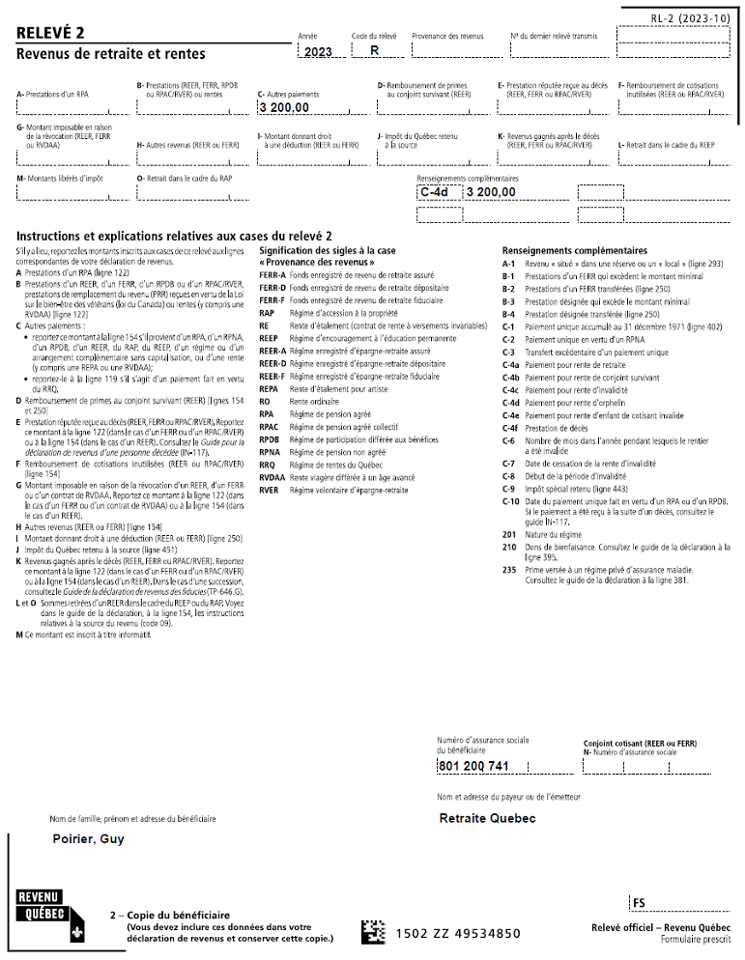
\includegraphics[width=.9\textwidth]{exercice/7-2/Q2/RL2.png}
		\caption[]{Exercice 2, Relevé~2}
		\label{fig:chap7Exercice2RL2}
	\end{figure}
\end{question}
Le Relevé~2 est au nom de Guy Poirier. La case~C-4d du Relevé~2 indique qu'il a reçu des prestations d'orphelin. Il doit déclarer le montant sur ses déclarations T1 ligne~11400 et TP-1 ligne~119.


\begin{question}
	Stéphane Santerre a reçu le T4E(Q), figure~\ref{fig:chap7Exercice2T4EQ}.
	\begin{figure}
		\centering
		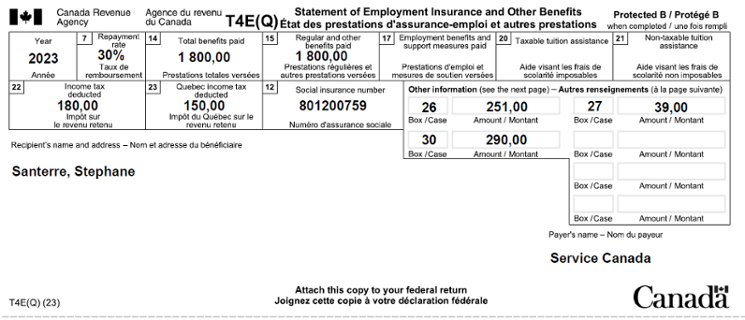
\includegraphics[width=.9\textwidth]{exercice/7-2/Q3/T4EQ.png}
		\caption[]{Exercice 2, T4E(Q)}
		\label{fig:chap7Exercice2T4EQ}
	\end{figure}
\end{question}
\setcounter{sousQuestion}{0}
\begin{sousQuestion}
	Que signifient les montants dans les cases~26, 27 et 30 du feuillet~T4E?
\end{sousQuestion}
Le montant inscrit à la case~26 représente un trop-perçu qui a été recouvré alors que Stéphane percevait des prestations d'assurance-emploi. Il est également inclus dans le montant de la case~30.

Le montant inscrit à la case~27 représente l'annulation de l'impôt retenu pour le montant inscrit à la case~26. Il est également inclus dans le montant de la case~30.

Le montant de la case~30 représente le total des remboursements effectués par Stéphane pendant qu'il percevait les prestations. Ce montant correspond au total des cases~26 et 27.

\begin{sousQuestion}
	Comment traitez-vous ces informations sur les déclarations de Stéphane?
\end{sousQuestion}
Les \numprint{1800}~\$ de prestations versées à Stéphane Santerre doivent être reportées comme revenu aux lignes~11900 de la T1 et 111 de la TP-1. Quant aux 290~\$ qui ont été remboursés, une déduction correspondante peut être réclamée, au fédéral, à la ligne~23200 de la T1, en indiquant qu'il s'agit de prestations d'assurance-emploi remboursées. Au Québec, cette déduction peut être réclamée à la ligne~246 de la TP-1.

\begin{question}
	Le revenu net avant rajustements de Stéphane Santerre (Q3) est de \numprint{77375}~\$.
\end{question}
\setcounter{sousQuestion}{0}
\begin{sousQuestion}
	Quel est le seuil au-dessus duquel il est obligé de rembourser une partie de ses prestations d'assurance-emploi?
\end{sousQuestion}
Le seuil est de \numprint{76875}~\$.

\begin{sousQuestion}
	Calculez le montant du remboursement des prestations d'AE de Stéphane en utilisant la grille du \href{https://www.canada.ca/fr/agence-revenu/services/formulaires-publications/formulaires/t4e.html}{T4E}, cf.~figure~\ref{fig:chap7Exercice2T4E}.
	\begin{figure}
		\centering
		\includegraphics[width=.9\textwidth]{exercice/7-2/Q4/T4E.png}
		\caption[]{Exercice 2, T4E(Q), Tableau de remboursement}
		\label{fig:chap7Exercice2T4E}
	\end{figure}
\end{sousQuestion}
Le remboursement des prestations sociales de Stéphane est de 150~\$, tel que calculé dans la grille de remboursement, cf.~igure~\ref{fig:chap7Exercice2T4ERep}.
\begin{figure}
	\centering
	\includegraphics[width=.9\textwidth]{exercice/7-2/Q4/T4EReponse.png}
	\caption[]{Exercice 2, T4E(Q), Tableau de remboursement, rempli}
	\label{fig:chap7Exercice2T4ERep}
\end{figure}
\begin{sousQuestion}
	À quelles lignes de sa T1 et de sa TP-1, ce remboursement doit-il être inscrit? 
\end{sousQuestion}
Au fédéral, le montant doit être inscrit aux lignes~23500 et 42200 de la T1. Au Québec, il doit l'être à la ligne~250, code \og 03\fg{} à la case~249 de la TP-1.



\section{Paiements et remboursements rétroactifs des prestations liées à la COVID-19}
Les programmes d'aide COVID-19 ont pris fin, mais il est toujours possible de recevoir des paiements rétroactifs en 2023. Tous ces avantages sont imposables dans l'année où ils sont reçus, donc tout revenu reçu en 2023 est déclaré sur un feuillet~T4A de 2023 dans l'une des cases suivantes:
\begin{itemize}
	\item case~197: Prestation canadienne d'urgence (PCU);
	\item case~198: Prestation canadienne d'urgence pour les étudiants (PCUE);
	\item case~199: Prestation canadienne d'urgence pour les étudiants (PCUE) pour les étudiants handicapés admissibles ou ceux qui ont des enfants ou d'autres personnes à charge;
	\item case~200: Paiements d'aide financière provinciaux ou territoriaux liés à la COVID-19;
	\item case~202: Prestation canadienne de la relance économique (PCRE);
	\item case~203: Prestation canadienne de maladie pour la relance économique (PCMRE);
	\item case~204: Prestation canadienne de la relance économique pour proches aidants (PCREPA);
	\item case~211: Prestation canadienne pour les travailleurs en cas de confinement (PCTCC).
\end{itemize}

Chacun de ces avantages est déclaré à la ligne~13000 de la déclaration de revenus. Certaines de ces prestations comportaient une retenue d'impôt de 10~\% sur les paiements, mais d'autres n'ont pas retenu d'impôt. Si de l'impôt a été retenu, il est déclaré à la case~022 du feuillet~T4A. 


\subsection{Remboursements des prestations COVID}
De nombreux contribuables ont reçu des prestations auxquelles ils n'avaient pas droit et les ont remboursées par la suite. Si le montant a été reçu et remboursé en 2024, le revenu déclaré sur le feuillet~T4A de 2024 est réduit proportionnellement. Si un revenu a été reçu en 2020 ou 2021 et n'a été remboursé qu'en 2023, il peut être demandé comme déduction dans la déclaration de revenus de 2023. Le remboursement de la prestation liée à la COVID est inscrit comme déduction à la ligne~23200.

Les prestations qui ont été remboursées dans une année différente de celle où elles ont été reçues sont indiquées à la case~201 du feuillet~T4A si les prestations ont été demandées par l'intermédiaire de l'ARC. Si elles ont été demandées par l'intermédiaire de Service Canada, elles sont incluses à la case~30 du feuillet~T4E avec toutes les prestations d'assurance-emploi qui ont été remboursées. Service Canada enverra au bénéficiaire une lettre indiquant le montant lié à la PCU.



\section{Autres revenus}
\begin{intro}
	La plupart des autres revenus, c'est-à-dire les revenus qui n'ont pas à être déclarés à une ligne spécifique des déclarations de revenus, doivent être déclarés à la ligne~13000 de la T1 et à la ligne~154 de la TP-1. Sur cette page, vous verrez des revenus moins communs. La plupart des revenus énumérés ci-dessous sont à inscrire aux lignes~13000 de la T1 et à la ligne~154 de la TP-1 à moins d'indication contraire.
\end{intro}


\subsection{Gains d'un vol ou d'un détournement de fonds}
Tous les montants reçus à la suite d'activités criminelles doivent être inclus dans le revenu. Si les biens reçus sont des biens autres que des espèces, leur juste valeur marchande doit être incluse comme revenu. Si le contribuable rembourse des montants qu'il a inclus auparavant dans son revenu, il peut réclamer une déduction pour le montant remboursé aux lignes~23200 de la déclaration T1 et 250, code \og 17 \fg{} à la case~249, de la déclaration~TP-1.


\subsection{Prestation consécutive au décès}
La prestation consécutive au décès est un montant payé à l'époux ou conjoint de fait, ou à toute autre personne, à la suite du décès d'un employé en reconnaissance des années de services de ce dernier. Au provincial, elle est désignée sous l'appellation \og prestation au décès \fg{} (Ne pas confondre avec la prestation de décès).

Les prestations consécutives au décès sont inscrites aux cases~106 du T4A et O du relevé~1. Au Québec, le code \og RK \fg{} est indiqué à la case Code (case~O) du relevé~1. Elles peuvent aussi être inscrites aux cases~26 du T3 et G du relevé~16.

Les premiers \numprint{10000}~\$ d'une prestation consécutive au décès sont exonérés d'impôt. Cela réduit le montant à déclarer. Cette réduction pouvant aller jusqu'à \numprint{10000}~\$ du montant brut est versée à l'époux(se) ou au conjoint(e) de fait survivant ou à d'autres bénéficiaires. Seul le montant net doit être déclaré à la ligne~13000 de la T1 en spécifiant \og Prestation de décès \fg{} à cette ligne, et à la ligne~154 de la déclaration~TP-1, en utilisant le code 03 à la case~153. 

\subsubsection{Répartition de l'exemption de \numprint{10000}~\$ entre les bénéficiaires}
Au fédéral, lorsqu'il n'y a qu'une seule bénéficiaire, il est relativement facile de calculer le montant qui n'est pas imposable. En effet, on soustrait tout simplement l'exemption de \numprint{10000}~\$ du montant total reçu. Toutefois:

\begin{itemize}
	\item Lorsqu'il y a un(e) conjointe survivant(e) et un autre bénéficiaire ou plus, l'exemption doit être réclamée en premier par la/le conjoint(e) survivant(e) et le reste par les autres personnes.
	\item S'il n'y a aucun(e) conjoint(e) survivant(e) et que des prestations consécutives au décès ont été versées à plus d'une personne, tous les bénéficiaires de la prestation doivent se partager l'exemption maximale, selon la proportion du montant reçu par chacun.
\end{itemize}

Au Québec, l'exemption de \numprint{10000}~\$ doit être répartie proportionnellement aux montants reçus, même si l'un des bénéficiaires de la prestation au décès est le/la conjoint(e) survivant(e).


\subsection{Supplément d'un programme gouvernemental d'incitation au travail}
Il s'agit d'un supplément de revenu que le contribuable a reçu dans le cadre d'un programme gouvernemental d'incitation au travail. Au Québec, les montants sont versés à titre de soutien financier par le ministère de l'Emploi et de la Solidarité sociale. Ils doivent être inclus dans le revenu du bénéficiaire, tant au fédéral qu'au Québec. 

Au fédéral, les montants versés sont inscrits à la case~028 du T4A et reportés à la ligne~13000 de la T1. Au Québec, les sommes versées sont indiquées à la case~O du relevé~1, code \og RS \fg{} à la Code (case~O), et elles sont reportées à la ligne~154, code \og 02 \fg{} à la case~153, de la TP-1.

Le supplément reçu dans le cadre du Programme gouvernemental d'incitation au travail est considéré comme un revenu de travail, au même titre que les montants reçus à titre de traitement ou de salaire, dans:
\begin{itemize}
	\item Le calcul de la déduction pour produits et services de soutien à une personne atteinte d'une déficience, au fédéral et au Québec;
	\item Le calcul de la déduction pour travailleur réclamée au Québec et le calcul du montant canadien pour emploi réclamé au fédéral;
	\item Le calcul du crédit d'impôt pour prolongation de carrière, au Québec.
\end{itemize}


\subsection{Participation à des essais cliniques}
Certaines sociétés pharmaceutiques recrutent des gens via des annonces dans les journaux pour tester des médicaments et versent des indemnités en argent aux participants. Selon l'ARC et Revenu Québec, ces indemnités sont imposables à titre de revenu d'emploi ou d'entreprise, selon le cas.

Au Québec, les premiers \numprint{1500}~\$ d'une indemnité reçue par un participant à des essais cliniques ne sont pas imposables. Une déduction peut donc être réclamée à la ligne~250, code \og 17 \fg{} à la case~249, de la TP-1.

Cette déduction correspond au moins élevée des montants suivants: \numprint{1500}~\$ ou le montant inclus dans le calcul du revenu du contribuable à titre d'indemnité reçue pour sa participation à des essais cliniques. 

Le fédéral n'accorde pas une telle déduction.


\subsection{Allocation canadienne aux parents de jeunes victimes de crimes}
L'allocation canadienne aux parents de jeunes victimes de crimes offre des compensations aux parents qui ont dû s'absenter du travail pour faire face à la mort ou la disparition d'un enfant en raison d'une infraction ou d'une infraction probable au Code criminel.

Les subventions offrent 450~\$ en soutien de revenu par semaine, jusqu'à 35 semaines. Afin d'être admissibles, les parents doivent avoir gagné un minimum de \numprint{6500}~\$ dans l'année civile précédente ou dans les 52 dernières semaines et ont dû s'absenter de leur emploi.

Le montant sera identifié dans la case~136 du T4A et à la case~O du relevé~1 (identifié par le code \og CD \fg{}). Il doit être inclus dans le revenu aux lignes~13000 de la T1 et 154, avec le code 03 à la case~153, de la TP-1.


\subsection{Autres montants}
Les divers montants suivants sont également déclarés aux lignes~13000 de la T1 et 154 de la TP-1.


\subsection{Paiements rétroactifs provenant d'autres sources}
Le contribuable peut choisir que certains paiements rétroactifs provenant de sources soient imposés comme s'ils avaient été reçus dans l'année pour laquelle ils étaient censés être payés.
\begin{itemize}
	\item Les bourses d'études, de perfectionnement ou toute aide financière semblable qui n'est pas exemptée d'impôt;
	\item Les allocations de retraite et de départ;
	\item Les paiements forfaitaires d'un \acrshort{rpa} ou d'un \acrshort{rpdb}; 
	\item Certains paiements reçus d'un \acrfull{reee};
	\item Les sommes reçues en vertu d'une convention de retraite;
	\item Tout autre revenu imposable qui n'est pas inscrit sur une autre ligne.
\end{itemize}



\section{Autres déductions}
\begin{intro}
	Tout remboursement effectué dans l'année d'imposition en cours pour un revenu déclaré au cours de l'année ou des années précédentes peut être réclamé en déduction. Il est possible que ces remboursements réduisent le revenu de l'année précédente au lieu de celui de l'année en cours.
\end{intro}


\subsection{Remboursement de sommes déclarées comme revenu}
Il arrive parfois que certains revenus doivent être remboursés pour diverses raisons (par exemple, non-admissibilité, fraude, etc.). Tout remboursement d'un montant qui a été déclaré comme revenu dans l'année courante ou dans une année antérieure peut être déduit dans l'année du remboursement.

Au fédéral, une déduction peut être réclamée à la ligne~23200 de la T1. Au Québec, elle peut être réclamée à la ligne~246 de la TP-1.

Si le contribuable a reçu un salaire ou des prestations d'assurance salaire durant une période où il n'exerçait pas les fonctions afférentes à son emploi et qu'il a dû les rembourser, ils peuvent être déduits aux lignes~22900 de la T1 et 207, code \og 12 \fg{} à la case~206, de la TP-1. Il faut toutefois que le contribuable les ait inclus dans son revenu pour l'année en cours ou pour une année antérieure. 


\subsection{Déduction ou crédit d'impôt remboursable -- Québec}
Si, en 2023, un contribuable a remboursé un montant qu'il a reçu au cours d'une année antérieure en vertu du RRQ ou du RQAP, il peut demander à Revenu Québec de calculer s'il est plus avantageux pour lui de ne pas utiliser le remboursement pour réduire le revenu de l'année précédente et de se voir plutôt accorder un crédit d'impôt dans l'année courante pour l'étalement de la déduction à la ligne~462 de sa déclaration~TP-1. 

Dans une telle situation, le contribuable doit reporter le montant du remboursement à la ligne~246 de sa TP-1, ainsi à la ligne~462, code \og 08 \fg{} à la case~461. Il doit joindre à sa déclaration provinciale une note précisant l'année visée par le remboursement et les documents justifiant ce remboursement. Revenu Québec accordera le crédit d'impôt, si c'est plus avantageux pour le contribuable.



\section{Frais juridiques}
\begin{intro}
	Un ensemble limité de frais juridiques peut être réclamé à titre de déduction. La raison pour laquelle les frais juridiques ont été encourus détermine sur quelle ligne la déduction peut être réclamée.
\end{intro}

Les frais juridiques suivants peuvent être réclamés à la ligne~22900 de la T1 et à la ligne~207, code \og 09 \fg{} à la case~206, de la TP-1:

\begin{itemize}
	\item Les frais juridiques payés pour percevoir ou établir le droit à un salaire ou un traitement, ou pour établir un droit à ceux-ci. Même si le contribuable ne reçoit aucun montant dans l'année, cela ne l'empêche pas de déduire les frais payés s'il est établi qu'une somme lui est due:
	\begin{itemize}
		\item Le montant admissible à la déduction est le coût payé moins tout parti de ce montant qui a été accordé par le tribunal. Si les frais sont remboursés ou accordés par le tribunal au cours de l'année suivante, ils doivent être ajoutés aux revenus pour l'année où ils ont été reçus;
		\item Un contribuable peut déduire les frais juridiques payés pour recouvrer un montant qui lui est dû ou pour établir un droit à des montants qui, s'il les recevait, seraient inclus dans son revenu d'emploi même s'ils ne sont pas payés directement par son employeur;
	\end{itemize}
	\item Les frais juridiques payés pour percevoir une prestation d'assurance salaire (à laquelle l'employeur contribuait) ou pour établir un droit à celle-ci.
\end{itemize}

Par ailleurs, les frais juridiques suivants sont déductibles à la ligne~23200 de la T1 et 250, code \og 08 \fg{} à la case~249, de la TP-1:

\begin{itemize}
	\item Les frais juridiques payés par le contribuable pour des services de consultation et d'aide (y compris tous les frais comptables connexes) pour répondre à l'ARC et à Revenu Québec lorsqu'ils vérifient ses revenus, déductions ou crédits pour une année donnée;
	\item Les honoraires ou les frais engagés pour préparer, présenter ou poursuivre une opposition ou pour faire appel concernant une cotisation établie ou une décision prise selon la \textbf{Loi de l'impôt sur le revenu}, la \textbf{Loi sur les impôts au Québec}, la \textbf{Loi sur l'assurance-emploi} et le \textbf{Régime de rentes du Québec};
	\item Les frais juridiques payés pour obtenir ou recouvrer une allocation de retraite ou une prestation de retraite ou pour établir un droit à l'une de celles-ci jusqu'à concurrence des sommes reçues dans l'année, moins toute partie de ces montants qui auraient pu être transférés à un régime de retraite;
	\item Toute fraction non déduite peut être reportée aux sept années suivantes.
\end{itemize}


\subsection{Frais juridiques non déductibles}
Les frais juridiques qui ne peuvent pas être réclamés comprennent notamment:
\begin{itemize}
	\item Les frais engagés pour se défendre contre des accusations au civil / criminel;
	\item Les frais engagés pour faire l'acquisition d'une immobilisation (ces frais sont utilisés pour augmenter le prix de base rajusté du bien).
\end{itemize}



\section{Déductions supplémentaires}
\begin{intro}
	Après avoir déterminé le revenu net aux lignes~23600 de la T1 et 275 de la TP-1, le contribuable peut réclamer d'autres déductions lors du calcul de son revenu imposable.
\end{intro}


\subsection{Déduction pour revenu non imposable selon une convention fiscale}
Le contribuable peut réclamer une déduction à la ligne~25600 de la T1 et à la ligne~297, code \og 12 \fg{} à la case~296, de la TP-1 pour un revenu de source étrangère qui est non imposable au Canada selon une convention fiscale. Pour réclamer la déduction, il doit avoir inclus le montant reçu dans ses revenus. Il peut s'agir de revenus étrangers de placement ou de retraite.


\subsection{Vœu de pauvreté perpétuelle}
Au fédéral, le membre d'un ordre religieux qui a prononcé des vœux de pauvreté perpétuelle peut donner son revenu gagné et son revenu de pension à cet ordre. Par contre, il peut réclamer une déduction correspondante à la ligne~25600 de sa T1.

Pour avoir droit à cette déduction, le contribuable doit avoir donné tout revenu gagné à l'ordre religieux et non seulement une partie de celui-ci. Ceci remplace le crédit pour dons de bienfaisance qui est discuté plus loin dans ce chapitre. Il doit joindre une lettre de sa communauté ou de son employeur attestant son vœu de pauvreté perpétuelle. 

Il n'y a pas de déduction équivalente pour le Québec. 


\subsection{Aide visant les frais de scolarité pour la formation de base des adultes}
Un contribuable qui a inclus dans ses revenus une aide financière pour couvrir une partie ou la totalité des frais de scolarité qu'il a payés pour suivre des cours de niveau primaire ou secondaire peut réclamer une déduction pour le montant de l'aide reçue. 

Cette aide figure à la case~21 de son T4E et elle est incluse dans le montant de la case~14. Cette déduction peut être réclamée à la ligne~25600 de la déclaration T1 et à la ligne~295 de la déclaration~TP-1. 


\subsection{Déductions spécifiques au Québec}
Les déductions suivantes peuvent être réclamées à la ligne~297 de la TP-1: voir table~\ref{table:deductionsSupplementairesSpecifiquesAuQuebec}.
\begin{table}
	\centering
	\begin{tabular}{|l|c|c|}
		\hline
		\multicolumn{3}{|c|}{La déduction s'inscrit à la ligne~297 de la TP-1}                                      \\
		\multicolumn{3}{|c|}{Le code s'inscrit à la case~296}                                                       \\
		\multicolumn{3}{|c|}{Le taux d'exemption se trouve à la case~A-14 du RL-1 (s'il y a lieu)}                  \\ \hline
		\textbf{Description}                                     & \textbf{Code} &      \textbf{Montant de la}      \\
		                                                         & \textbf{case} &     \textbf{déduction à la}      \\
		                                                         & \textbf{296}  &      \textbf{case~Du RL-1}       \\ \hline
		Déduction pour chercheur étranger*                       &      03       &               A-10               \\ \hline
		Déduction pour expert étranger*                          &      04       &               A-12               \\ \hline
		Déduction pour chercheur étranger en stage postdoctoral* &      05       &               A-11               \\ \hline
		Déduction pour spécialiste étranger*                     &      06       &               A-9                \\ \hline
		Déduction pour revenu d'emploi gagné sur un navire       &      08       &               A-6                \\ \hline
		Déduction pour professeur étranger                       &      19       &               A-13               \\ \hline
		Déduction pour le personnel des Forces canadiennes et    &      23       &               A-7                \\
		des forces policières                                    &               &                                  \\ \hline
		Déduction pour remboursement d'une prestation            &      24       &             case~12              \\
		universelle pour garde d'enfants                         &               &             du RC62              \\ \hline
		Déduction pour remboursement d'une prestation d'un       &      25       &              s. o.               \\
		régime enregistré d'épargne-invalidité                   &               &                                  \\ \hline
		\multicolumn{3}{|l|}{*La déduction disponible doit être réduite de la somme des montants des cases~105,}    \\
		\multicolumn{3}{|l|}{205 et 207 associés aux revenus admissibles à cette déduction, multipliée par le taux} \\
		\multicolumn{3}{|l|}{de la case~A-14.}                                                                      \\ \hline
	\end{tabular}
	\caption{Déductions supplémentaires spécifiques au Québec}
	\label{table:deductionsSupplementairesSpecifiquesAuQuebec}
\end{table}

\rqg[s]{47 à 49}



\section{Achat d'une habitation}
\begin{intro}
	Les acheteurs d'une première maison peuvent réclamer un crédit d'impôt non remboursable d'un montant de \numprint{10000}~\$ (augmentation de \numprint{5000}~\$ par rapport à 2023) pour l'achat d'une habitation admissible qu'ils ont acquise dans l'année d'imposition.
\end{intro}

Pour réclamer le crédit d'impôt, les conditions suivantes doivent être respectées:
\begin{itemize}
	\item Le contribuable ou sa conjointe (épouse ou de fait) a fait l'acquisition d'une habitation admissible; 
	\item Le contribuable n'a pas habité, au cours de l'année d'acquisition ou des quatre années précédentes, dans une autre habitation dont lui-même ou sa conjointe (épouse ou de fait) était propriétaire;
	\item Le contribuable sera admissible au crédit d'impôt si sa conjointe (épouse ou de fait) était propriétaire d'une habitation pendant la période en question. Toutefois, le contribuable ne peut y avoir vécu pendant qu'ils étaient mariés ou en union de fait.
\end{itemize}

Une \og habitation admissible \fg{} comprend les maisons unifamiliales, les maisons semi-détachées, les maisons en rangée, les maisons mobiles, les habitations en copropriété (condominiums), les appartements dans un duplex, un triplex, un quadruplex ou un immeuble, et les parts dans une coopérative d'habitation en tant que propriétaire. Il peut s'agir aussi d'une habitation existante ou en construction.

Cette habitation doit être située au Canada et enregistrée au nom du contribuable et à celui de son époux(se) ou conjoint(e) de fait.

Les documents justificatifs doivent inclure:
\begin{itemize}[label=\twemoji{check box with check}]
	\item Le nom de l'acheteur;
	\item La date de clôture de la transaction;
	\item L'adresse de la propriété;
	\item Si l'habitation est achetée pour une personne handicapée;
	\item La date d'acquisition de l'habitation.
\end{itemize}

Les époux ou conjoints de fait peuvent se partager le montant entre eux quel que soit le nom qui figure sur l'enregistrement de la maison. Si plus d'une personne a droit au montant, le montant total que les personnes peuvent réclamer pour l'année ne doit pas dépasser le montant total du crédit.

Le montant pour l'achat d'une habitation peut aussi être réclamé à l'égard de certaines habitations acquises par les personnes admissibles au crédit d'impôt pour personnes handicapées ou au bénéfice de ceux-ci si l'acquisition leur permet de vivre dans une habitation plus accessible ou dans un environnement mieux adapté à leurs besoins personnels et leurs soins. Un contribuable n'a pas à être l'acheteur d'une première habitation s'il a droit au montant pour personnes handicapées ou s'il fait l'acquisition d'une habitation au bénéfice d'un parent qui y a droit.


\subsection{Le crédit d'impôt}
Le crédit d'impôt non remboursable pour l'achat d'une habitation est de \numprint{10000}~\$ au fédéral et de \numprint{10000}~\$ au Québec.

Au fédéral, le crédit d'impôt de \numprint{10000}~\$ s'inscrit à la ligne~31270 de la T1. Bien entendu, le taux de 15~\% sera appliqué pour obtenir un crédit d'impôt net de \numprint{1500}~\$.

Au Québec, le crédit d'impôt est calculé sur le formulaire TP-752.HA. Le crédit d'impôt maximum résultant de ce calcul est de \numprint{1500}~\$. Ce montant sera inscrit à la ligne~396 de la TP1.

\qct\href{https://www.revenuquebec.ca/fr/services-en-ligne/formulaires-et-publications/details-courant/tp-752-ha/}{TP-752.HA -- Crédit d'impôt pour achat d'une habitation}

\subsubsection{Informations supplémentaires pour la TP-1}
Contrairement à la réclamation fédérale sur la T1, le contribuable ne peut pas simplement réclamer \numprint{1500}~\$ ou sa part du crédit.

Dans le calcul dans le TP.752.HA, le montant qui peut être réclamé dépend de la différence entre l'impôt sur le revenu imposable à la ligne~401 moins la somme des crédits non remboursables des lignes~359 à 367 multipliée par 15~\% moins les montants demandés aux lignes~391 et 397.

En effet, le montant du crédit d'impôt pour l'achat d'une habitation est limité au montant requis pour réduire l'impôt sur le revenu imposable à zéro ou jusqu'au maximum de \numprint{1500}~\$.

Si le contribuable dispose déjà de suffisamment de crédits non remboursables pour réduire à zéro l'impôt sur le revenu imposable, aucun crédit d'impôt pour achat d'une habitation ne sera accordé.

Il est donc possible que le contribuable ne puisse pas réclamer sa juste part du crédit.

Par conséquent, ils devraient envisager de laisser à l'autre co-acheteur une plus grande part des \numprint{1500}~\$ si cela est plus efficace sur le plan fiscal pour eux.



\section{Nouvelles numériques}
\begin{intro}
	Un contribuable admissible qui a payé des frais pour un abonnement aux nouvelles numériques à une organisation journalistique canadienne qualifiée peut réclamer un crédit d'impôt non remboursable pour les montants engagés.
\end{intro}

Il s'agit d'un crédit temporaire admissible sur la T1 pour les années d'imposition de 2020 à 2024. Le contribuable ne peut pas réclamer plus de 500~\$ et doit être inscrit à la ligne~31350 de la T1.

Afin d'être admissible au crédit, l'abonnement doit être fait à une \og \acrfull{ojcq} \fg{} qui se consacre principalement à la production de contenu original de nouvelles écrites. Les organismes engagés de quelque manière que ce soit dans la radiodiffusion ne seront pas admissibles.

\cat\href{https://www.canada.ca/fr/agence-revenu/services/impot/particuliers/sujets/tout-votre-declaration-revenus/declaration-revenus/remplir-declaration-revenus/deductions-credits-depenses/toutes-deductions-tous-credits-toutes-depenses/abonnement-aux-actualites-numeriques/liste-abonnements-nouvelles-numeriques-admissibles.html}{Liste des abonnements aux nouvelles numériques admissibles}

La définition d'une OJCQ est longue et technique. Cependant, il y a trois conditions particulièrement importantes:
\begin{itemize}
	\item Son contenu doit être édité et conçu au Canada;
	\item Elle doit être principalement engagée dans la production de contenus d'actualités originaux qui:
	\begin{itemize}
		\item Doit être principalement axé sur des questions d'intérêt général et des rapports sur l'actualité, y compris la couverture des institutions et processus démocratiques, et
		\item Ne doit pas être principalement axé sur un sujet particulier comme des nouvelles spécifiques à l'industrie, les sports, les loisirs, les arts, le style de vie ou le divertissement.
	\end{itemize}
	\item Elle n'est pas engagée de manière significative dans la production de contenu qui:
	\begin{itemize}
		\item Fait la promotion des intérêts ou rend compte des activités d'une organisation, d'une association ou de ses membres,
		\item Est produit pour un gouvernement, une société d'État ou un organisme gouvernemental, ou
		\item Fais la promotion de biens et services.
	\end{itemize}
\end{itemize}



\section{Dons}
\begin{intro}
	Un contribuable qui fait un don d'argent ou de biens à des organismes de bienfaisance enregistrés peut avoir droit à un crédit d'impôt non remboursable pour ce don, au fédéral et au Québec. Il peut ainsi réclamer le montant admissible d'un don qu'il a fait en 2023 et au cours des années 2018 à 2022, s'il n'a jamais réclamé de crédit pour ces derniers.
\end{intro}


\subsection{Don de bienfaisance}
Le crédit d'impôt, pour un don justifié par un reçu officiel, s'inscrit à la ligne~34900 de la T1 et à la ligne~395 de la TP-1. 

Au fédéral, le montant admissible des dons ne doit pas dépasser 75~\% du revenu net (ligne~23600 de la T1). Au Québec, il n'y a pas de limite.

\subsubsection{Reçu et montant admissible d'un don}
Un reçu pour don doit porter le nom de l'organisme de bienfaisance ainsi que son numéro d'entreprise, lequel a été obtenu auprès de l'ARC ou de Revenu Québec. Le nom et l'adresse complète du donateur doivent aussi y être clairement indiqués. De plus, le reçu doit être signé par un responsable dûment autorisé de l'organisme de charité, et il doit être numéroté.

Au fédéral seulement, le reçu doit porter le nom \og Agence de revenu du Canada \fg{}, qu'il soit écrit à la main ou au moyen d'un autocollant ou d'une estampe. Le reçu doit également indiquer le \og montant admissible \fg{} du don. 

Le don prélevé à la source par l'employeur apparaît aux cases~46 et N des T4 et relevé~1. Aucun reçu officiel requis.

Un don peut aussi être prélevé:
\begin{itemize}
	\item À la case~46 du T4A et à la case~210 du relevé~2;
	\item À la case~48 du T3 et à la case~N du relevé~16;
	\item Aux cases~182 et 183 du T5013 et aux cases~19 et 20 du relevé~15;
	\item À la case~13 du T5003 et à la case~H du relevé~14.
\end{itemize}

Le contribuable doit conserver ses reçus de dons pour éléments de preuve.

Dans ce cours, nous nous concentrons sur les dons en argent plutôt que sur les dons en nature qui sont plus complexes pour déterminer le traitement fiscal.

Il est possible que certains organismes prétendent être des organismes de bienfaisance. S'ils ne sont pas enregistrés auprès de l'ARC, un crédit d'impôt ne peut être réclamé.

\cat\href{https://apps.cra-arc.gc.ca/ebci/hacc/srch/pub/dsplyBscSrch}{Liste des organismes de bienfaisance et de certains autres donataires reconnus -- Recherche de base}


\subsection{Dons admissibles}
Courte liste d'organismes de bienfaisance enregistrés:
\begin{itemize}
	\item La Société canadienne de la croix rouge;
	\item Centraide;
	\item La Société canadienne du cancer;
	\item L'Armée du salut;
	\item Le YMCA et le YWCA;
	\item Les scouts et les guides;
	\item Les églises, temples, synagogues et autres;
	\item La Fondation canadienne des maladies du cœur et autres fondations;
	\item Les écoles sans but lucratif, les collèges, les universités, les bibliothèques et les musées.
\end{itemize}

Un don octroyé à une école réservée à l'instruction religieuse, à une école autre qu'un établissement postsecondaire ou un établissement scolaire désigné est admissible comme don de charité, mais non comme frais de scolarité. Le don octroyé pour l'enseignement religieux dans des institutions d'enseignement primaire et secondaire est admissible au fédéral seulement.

\begin{note}
	La catégorie d'\acrfull{oje} a été ajoutée pour 2020. Au Québec, deux OJE:
	\begin{itemize}
		\item La Presse inc.: média numérique indépendant dont la mission est d'offrir une information de qualité, gratuite et accessible à tous;
		\item Journaldesvoisins.com: journal indépendant, communautaire, professionnel et quotidien d'informations locales.
	\end{itemize}
\end{note}

\subsubsection{Dons admissibles seulement au Québec}
Au Québec seulement, un contribuable peut réclamer:
\begin{itemize}[label=\twemoji{check mark button}]
	\item Le don offert à un organisme d'éducation politique ou à un organisme artistique reconnu par le Ministre du Revenu du Québec;
	\item Le don offert à l'Agence de la Francophonie ou à l'un de ses organismes subsidiaires;
	\item Le don d'un instrument de musique, offert après le 23 mars~2006, à un établissement d'enseignement reconnu;
	\item Le don de biens culturels offert au Musée national des beaux-arts du Québec, au Musée d'Art contemporain de Montréal et au Musée de la civilisation;
	\item Le don d'une denrée alimentaire offert par une entreprise agricole.
\end{itemize}


\subsection{Dons non admissibles}
\begin{itemize}[label=\twemoji{cross mark}]
	\item Le don fait à des organisations de bienfaisance hors du Canada, sauf aux organisations désignées par les gouvernements;
	\item Le don fait à un contribuable;
	\item La valeur des services rendus;
	\item La valeur des marchandises dont le coût est imputé à une dépense d'entreprise 
	\item Le don de vêtements, mobiliers ou autres, à un organisme non enregistré;
	\item Le montant payé pour des billets à l'occasion de parties de cartes, bingos, loteries ou autres;
	\item Le don fait aux organisations patriotiques, fraternelles ou de secours mutuels; ou
	\item Au Québec, le don pour l'enseignement religieux.
\end{itemize}


\subsection{Traitement fiscal}
Au fédéral, le crédit d'impôt est calculé sur l'annexe~9 - Dons, avant d'être reporté à la ligne~34900 de la T1.

Le crédit d'impôt pour une année d'imposition donnée est égal au total des montants suivants:
\begin{itemize}
	\item 15~\% sur la première tranche de 200~\$ de dons effectués dans l'année;
	\item 33~\% du moindre:
	\begin{itemize}
		\item Total des dons effectués dans l'année qui excèdent la première tranche de 200~\$,
		\item Revenu imposable de l'année qui excède le seuil du taux d'imposition supérieur des particuliers (\numprint{235675}~\$ en 2023);
	\end{itemize}
	\item 29~\% du total des dons effectués dans l'année, supérieurs à 200~\$ qui ne sont pas admissibles au taux de 33~\% mentionné ci-dessus.
\end{itemize}

Pour la TP-1, le contribuable doit utiliser la grille de calcul de la ligne~395 pour les dons monétaires au cours de l'année. Sinon, l'annexe~V doit être utilisée.

Le crédit d'impôt pour une année d'imposition donnée est égal au total des montants suivants:
\begin{itemize}
	\item 20~\% sur la première tranche de 200~\$ de dons effectués dans l'année;
	\item 25,75~\% du moindre:
	\begin{itemize}
		\item Total des dons effectués dans l'année qui excèdent la première tranche de 200~\$,
		\item Revenu imposable de l'année qui excède le seuil du taux d'imposition supérieur des particuliers (\numprint{119910}~\$ en 2023);
	\end{itemize}
	\item 24~\% du total des dons effectués dans l'année, supérieurs à 200~\$ qui ne sont pas admissibles au taux de 25,75~\% mentionné ci-dessus.
\end{itemize}


\subsection{Report des dons de bienfaisance}
Si les dons de bienfaisance ou autres dons ne réduisent pas à zéro l'impôt à payer, l'excédent peut être reporté sur les cinq années suivantes, sauf les dons de biens écosensibles et de biens culturels attestés faits après le 10~février~2014 sur 10~ans. En raison du délai de cinq ans, le report des années antérieures devrait être appliqué en premier lieu. Une note doit être jointe aux déclarations si le montant a été reporté d'une année précédente.


\subsection{Dons faits par l'époux ou le conjoint de fait}
L'une ou l'autre des personnes dans un couple marié ou en union de fait peut utiliser le reçu, peu importe à qui le reçu est établi. Les dons faits par les époux ou conjoints de fait peuvent être regroupés, afin de les réclamer sur une seule déclaration.

\subsection{Dons de biens}
Les dons de biens autres que l'argent peuvent être réclamés, pourvu qu'ils aient une certaine valeur. Par exemple, les dons de vieux vêtements ne sont pas admissibles puisqu'ils ont peu de valeur. 

\subsubsection{Dons de biens culturels}
Un bien culturel est:
\begin{itemize}
	\item Un bien canadien certifié par la \acrfull{cceebc}. La valeur du bien est inscrite sur le certificat T871, \textbf{Certificat fiscal visant des biens culturels}, émis par cet établissement; 
	\item Un bien québécois reconnu ou classé conformément à la \textbf{Loi sur le patrimoine culturel} ou à la Loi sur les biens culturels;
	\item Un bien pour lequel une \textbf{Attestation d'aliénation de biens culturels} (TPF-712.0.1) a été délivrée par le Conseil du patrimoine culturel du Québec, anciennement appelé Commission des biens culturels du Québec.
\end{itemize}

Pour être reconnu comme don de biens culturels, le don doit être fait à une administration publique ou un établissement prescrit. Le reçu officiel émis par le donataire ainsi que le certificat T871 ou l'attestation doivent être joints aux T1 et TP-1.

Une œuvre d'art créée par un artiste et comprise dans son inventaire, qui est offerte en donation, est un bien culturel. La juste valeur marchande de l'œuvre d'art en question, telle que déterminée par la CCEEBC, représente la valeur du don qui peut être réclamée.

Les dons de biens culturels attestés faits après le 10 février~2014, la juste valeur marchande du bien donné est réputée être le moins élevé des montants suivants:
\begin{itemize}
	\item La JVM déterminée du bien;
	\item Son coût immédiatement avant que le don soit fait.
\end{itemize}

Le montant admissible doit être inscrit à la ligne~34200 de l'annexe~9 (au fédéral) et à la partie 2 de l'annexe~V (au Québec). Le montant pouvant être réclamé n'est pas limité à un pourcentage du revenu net du contribuable (montant de la ligne~23600 de la T1 et du montant de la ligne~275 de la TP-1). 

\subsubsection{Dons d'une œuvre d'art au Québec}
Le don d'une œuvre d'art à un organisme de bienfaisance non relié au domaine des arts n'est admissible au crédit qu'au moment où l'organisme vend l'œuvre en question. La vente doit avoir lieu avant la fin de la cinquième année civile qui suit l'année du don.

C'est donc au moment de la disposition du bien que l'organisme en question remettra un reçu officiel et que le contribuable pourra réclamer le crédit. Si un reçu lui est délivré après la production de sa déclaration~TP-1, le contribuable doit faire une demande de redressement.

La mesure concernant la disposition du bien ne s'applique pas au don d'une œuvre d'art fait:
\begin{itemize}[label=\twemoji{cross mark}]
	\item au gouvernement fédéral, à une province, à une municipalité canadienne;
	\item à un organisme artistique reconnu par Revenu Québec;
	\item à un organisme qui a acquis l'œuvre d'art dans le cadre de sa mission première, aux dons de biens culturels et aux dons ayant une valeur patrimoniale.
\end{itemize}

Si le don d'une œuvre d'art a été fait à un musée situé au Québec ou à une institution muséale reconnue, le montant admissible du don est égal à 125~\% du montant servant au calcul du crédit.

\subsubsection{Dons d'une œuvre d'art public}
Afin d'inciter davantage les contribuables québécois à donner des œuvres d'art destinées à être installées à demeure dans des espaces publics ou des lieux réservés à l'enseignement, le montant admissible du don peut être majoré aux fins du calcul du crédit d'impôt pour dons sur la TP-1. Le don d'une œuvre d'art public doit être fait après le 3~juillet~2014.

Une \og œuvre d'art public \fg{} est une œuvre d'art à caractère permanent, souvent de grande dimension ou de type environnemental, installée dans un espace accessible à la population dans un but de commémoration, d'embellissement des lieux ou encore d'intégration à l'architecture ou à l'environnement de bâtiments et de sites à vocation publique.

Le crédit est augmenté de 25~\% à l'égard d'un don fait au gouvernement du Québec, à un organisme public ou à une municipalité québécoise. Le montant est majoré de 50~\% si l'œuvre acquise est installée dans un lieu d'enseignement situé au Québec.

La majoration du montant admissible d'un don d'une œuvre d'art public est calculée à la partie~A de l'annexe~V (lignes~6 et 8 dans le cas d'un don de bienfaisance et lignes~25 et 27 dans le cas d'un bien culturel).

\subsubsection{Dons de biens écosensibles}
Les dons de terrains, ou servitudes grevant un terrain, qui ont une valeur écologique reconnue par le ministre de l'Environnement, peuvent être admissibles, pourvu que le ministre fédéral de l'Environnement (et le ministère de l'Environnement du Québec pour un fonds de terre situé au Québec) ait certifié que la terre est vulnérable sur le plan environnemental et qu'il est important de la préserver et de la conserver pour protéger le patrimoine environnemental du Canada. Le montant peut être réclamé à la ligne~34200 de l'annexe~9 et à la ligne~22 de l'annexe~V. Il n'est pas limité à un pourcentage du revenu net.

Les dons de biens écosensibles peuvent être reportés jusqu'à 10 ans pour les dons faits à compter du 11~février~2014.

Au fédéral, depuis le 21~mars~2017, les dons de fonds de terre écosensibles ne sont plus admissibles au crédit d'impôt pour dons de bienfaisance, s'ils sont faits à une fondation privée. Ils continueront à être admissibles s'ils sont versés à un organisme de bienfaisance enregistré ou à d'autres donataires reconnus.

\subsubsection{Dons de denrées alimentaires au Québec}
Le montant admissible d'un don fait, après le 26~mars~2015, par un producteur agricole reconnu à un organisme de bienfaisance enregistré qui est soit Les Banques Alimentaires du Québec, soit un membre Moisson, peut être majoré de 50~\% aux fins du calcul de la déduction pour dons ou du crédit d'impôt non remboursable pour dons, selon le cas, si le don porte sur des produits agricoles admissibles.

Producteur agricole reconnu est une personne:
\begin{itemize}
	\item Sois qui exploite une entreprise enregistrée auprès du \acrfull{mapaq} à titre d'exploitation agricole;
	\item Soit un particulier membre d'une société de personnes qui exploite une telle entreprise et qui est membre de la société à la fin de son exercice financier.
	\item 
\end{itemize}

Produit alimentaire admissible:
\begin{itemize}[label=\twemoji{check mark button}]
	\item Viande ou sous-produit de viande;
	\item Œuf;
	\item Produits laitiers;
	\item Fruits;
	\item Légumes;
	\item Céréales;
	\item Légumineuses;
	\item Fines herbes;
	\item Miel;
	\item Sirop d'érable;
	\item Champignons;
	\item Noix;
	\item Etc.
\end{itemize}

\begin{note}
	Un produit transformé n'est pas admissible, sauf si sa transformation n'empêche pas qu'il soit légalement vendu, distribué ou mis en vente en dehors du lieu où il est produit, en tant que produit alimentaire ou boisson destinée à la consommation humaine.
\end{note}

Le contribuable qui a fait un don de denrées alimentaires qu'il transforme, après le 17~mars~2016, peut aussi demander un crédit d'impôt non remboursable pour dons. Le montant admissible de ce don peut être augmenté de 50~\% si, au moment du don, toutes les conditions suivantes étaient remplies:
\begin{itemize}
	\item Il exploite une entreprise de transformation d'aliments;
	\item Le don a été fait à un organisme de bienfaisance enregistré qui était Les Banques alimentaires du Québec, un membre Moisson ou un membre Associé;
	\item Les denrées alimentaires étaient des produits alimentaires admissibles.
\end{itemize}

Le montant peut être réclamé à la ligne~395 de la TP-1. Le contribuable doit remplir l'annexe~V.

\subsubsection{Crédit additionnel pour don important en culture -- Québec}
En plus du crédit d'impôt régulier pour dons de bienfaisance et autres dons calculés à la partie~A de l'annexe~V, un particulier peut avoir droit pour le même don à un crédit d'impôt additionnel pour don important en culture. Ce crédit est disponible si, après le 3~juillet~2013 et avant le 1\ier{}~janvier~2023, il a fait un don en argent d'au moins \numprint{5000}~\$ (effectué en un ou plusieurs versements) à l'un des donataires suivants:
\begin{itemize}
	\item Un organisme de bienfaisance enregistré œuvrant au Québec dans le domaine des arts ou de la culture;
	\item Un organisme culturel ou de communication enregistrée;
	\item Une institution muséale enregistrée, le Musée national des beaux-arts du Québec, le Musée d'art contemporain de Montréal, le Musée de la civilisation ou un musée qui est situé au Québec et constitué en vertu de la Loi sur les musées.
\end{itemize}

Le crédit additionnel est égal à 25~\% du montant admissible du don, jusqu'à l'occurrence d'un don de \numprint{25000}~\$. Il ne peut être réclamé qu'une seule fois. Il est calculé à la partie~B de l'annexe~V.

\subsubsection{Crédit pour dons de mécénat culturel -- Québec}
Un particulier peut demander un crédit d'impôt de 30~\% pour un don en argent d'au moins \numprint{250000}~\$ fait après le 3~juillet~2013 à un donataire admissible. Il s'agit des mêmes donataires qui sont reconnus aux fins du crédit d'impôt additionnel pour don important en culture. Le crédit est admissible même si le versement s'échelonne sur une période d'au plus dix ans, pourvu qu'un minimum de \numprint{25000}~\$ de dons soit fait par année et qu'une promesse de dons est enregistrée auprès du ministre de la Culture et des Communications.

Le crédit est calculé à la partie~C de l'annexe~V. 

Il ne s'agit pas d'un crédit supplémentaire. Ainsi, un contribuable ne pourra pas bénéficier du crédit d'impôt pour dons de bienfaisance et autres dons de la partie~A ni du crédit d'impôt additionnel pour don important en culture pour un don inscrit à la partie~C.

\subsection{Membres d'un ordre religieux}
Au fédéral, comme mentionné précédemment, les membres d'un ordre religieux qui ont prononcé des vœux de pauvreté perpétuelle peuvent donner tout leur revenu gagné à leur ordre. Par contre, ils peuvent réclamer une déduction de ce même montant à la ligne~25600 de leur T1 sans être restreints à la limite du revenu net. Tout leur revenu gagné doit être donné à cet ordre et non seulement une partie de celui-ci. Ils peuvent choisir de réclamer la déduction ou le crédit d'impôt non remboursable.

Au Québec, les membres d'un ordre religieux ayant fait vœu de pauvreté perpétuelle peuvent inscrire comme dons de bienfaisance les sommes remises à leur communauté religieuse jusqu'à concurrence de leur revenu net. 



\section{Exercice 3}
\setcounter{question}{0}
\begin{question}
	Suite au décès de son époux, Marjolaine a reçu \numprint{17000}~\$ de prestations consécutives au décès.
	
	À quelles lignes des déclarations doit-elle inscrire ces prestations? Quel montant doit-elle y inscrire?
\end{question}
Marjolaine doit inscrire \numprint{7000}~\$ (\numprint{17000}~\$ $–$ \numprint{10000}~\$) et \og Prestation consécutive au décès \fg{} à la ligne~13000 de sa T1; et à la ligne~154, code \og 03 \fg{} à la case~153, de sa TP-1.

\begin{question}
	En mars de l'année d'imposition, Micheline Latour a reçu un paiement forfaitaire rétroactif de \numprint{23000}~\$ de son plan de perte d'emploi, dont \numprint{10000}~\$ se rapporte à l'année précédente. Elle n'a jamais cotisé au régime.
\end{question}
\setcounter{sousQuestion}{0}
\begin{sousQuestion}
	Quel montant devrait-elle déclarer dans ses déclarations de revenus fédérale et provinciale pour l'année d'imposition en cours et sur quelles lignes?
\end{sousQuestion}
Micheline doit déclarer \numprint{23000}~\$ à la ligne~10400 de sa T1 et à la ligne~107 de sa TP1, en utilisant le code 02 à la case~106.

\begin{sousQuestion}
	Que doit-elle faire pour s'assurer que les \numprint{10000}~\$ relatifs à une année d'imposition précédente ne sont pas imposables dans l'année d'imposition en cours?
\end{sousQuestion}
Micheline peut demander à l'ARC et à RQ de calculer s'il est plus avantageux pour elle de reporter les \numprint{10000}~\$ à l'année d'imposition précédente. Elle doit faire la demande fédérale en joignant le formulaire T1198 à sa T1. Au Québec, elle doit cocher la case~404 de sa TP-1 et joindre le formulaire TP-766.2 à sa déclaration provinciale.

\begin{question}
	Bernard a payé des frais juridiques de 400~\$ afin de poursuivre son ancien employeur dans le but de récupérer \numprint{2000}~\$ de salaire non payé.
\end{question}
\setcounter{sousQuestion}{0}
\begin{sousQuestion}
	Il a gagné sa cause. En plus de récupérer le salaire qui lui est dû, le jugement de la cour lui a accordé 250~\$ pour couvrir une partie des frais juridiques payés.
	
	Quel montant peut-il déduire à titre de frais juridiques?
\end{sousQuestion}
Il peut déduire 150~\$, soit 400~\$ $-$ 250~\$.

\begin{sousQuestion}
	Si Bernard ne gagne pas sa cause et ne réussit pas à établir qu'un montant lui est dû, quel montant peut-il déduire à titre de frais juridiques au fédéral et au Québec?
\end{sousQuestion}
Même si Bernard ne gagne pas sa cause et ne parvient pas à établir que son employeur lui doit de l'argent, il peut déduire tous ses frais juridiques au Québec, mais pas au fédéral.

\begin{question}
	Indiquez si les dons énumérés ci-dessous sont des dons de bienfaisance admissibles ou non admissibles:
	\begin{enumerate}[label=\Alph*{}.]
		\item Don à la Société canadienne de la Croix-Rouge 	
		\item Don à une personne dans le besoin 	
		\item Don de vieux vêtements à un voisin 	
		\item Don au YMCA ou YWCA de la région 	
		\item Montant payé pour un bingo à l'église 	
		\item Don à l'église locale 	
		\item Don à un organisme religieux enregistré
	\end{enumerate}
\end{question}
\begin{enumerate}[label=\Alph*{}.]
	\item Admissible
	\item Non admissible
	\item Non admissible
	\item Admissible
	\item Non admissible
	\item Admissible
	\item Admissible
\end{enumerate}

\begin{question}
	Jean possède les reçus suivants pour les dons de bienfaisance en argent qu'il a offerts durant l'année d'imposition: table~\ref{table:chap7ex3Q5}.
	\begin{table}
		\centering
		\begin{tabular}{lcr}
			\textbf{Don}                 & \textbf{Date} &   \textbf{Montant} \\ \hline\hline
			Église interconfessionnelle  &     26-07     & \numprint{1700} \$ \\ \hline
			Société canadienne du cancer &     05-08     &             100 \$ \\ \hline
			Université de Montréal       &     02-09     &             150 \$ \\ \hline
			UNESCO                       &     16-10     &             200 \$ \\ \hline
			Scout Québec                 &     19-10     &              50 \$ \\ \hline
			Total des dons               &     31-12     & \numprint{2200} \$ \\ \hline
		\end{tabular}
		\caption[]{Exercice 3, dons}
		\label{table:chap7ex3Q5}
	\end{table}
	
	Ses revenus net et imposable au fédéral et Québec sont de \numprint{235908}~\$. Il désire réclamer le maximum au titre des dons de bienfaisance sur sa déclaration fédérale pour l'année d'imposition courante. C'est la première fois qu'il distribue des dons et qu'il réclame le crédit d'impôt. 
\end{question}
\setcounter{sousQuestion}{0}
\begin{sousQuestion}
	Complétez l'\href{https://www.canada.ca/fr/agence-revenu/services/formulaires-publications/trousses-impot-toutes-annees-imposition/trousse-generale-impot-prestations/5000-s9.html}{annexe~9}.
\end{sousQuestion}
Jean peut demander un crédit d'impôt de 619,32~\$, cf. figure~\ref{fig:chap7Exercice3Annexe9}.
\begin{figure}
	\centering
	\includegraphics[width=.9\textwidth]{exercice/7-3/Q5/Annexe9.png}
	\caption[]{Exercice 3, annexe~9}
	\label{fig:chap7Exercice3Annexe9}
\end{figure}

\begin{sousQuestion}
	Sur quelle ligne de la déclaration T1 Jean réclame-t-il le crédit?
\end{sousQuestion}
À la ligne~34900 de sa T1.

\begin{sousQuestion}
	Jean devrait-il utiliser la grille 395 ou l'annexe~V pour calculer le montant de dons qui peut être réclamé sur sa TP-1 du Québec?
\end{sousQuestion}
Jean n'a aucun montant reporté des années précédentes et tous ses dons sont faits à des organismes de bienfaisance enregistrés, il peut donc utiliser la grille de calcul~395.

\begin{sousQuestion}
	Remplissez la \href{https://www.revenuquebec.ca/documents/fr/formulaires/tp/2023-12/TP-1.D.GR%282023-12%29.pdf}{grille de calcul~395}, présentée ci-dessous, en supposant que son revenu imposable au Québec est également de \numprint{235908}~\$.
\end{sousQuestion}
Grille de calcul pour ligne~395: figure~\ref{fig:chap7Exercice3Grille395}.
\begin{figure}
	\centering
	\includegraphics[width=.9\textwidth]{exercice/7-3/Q5/Grille395.png}
	\caption[]{Exercice 3, Grille 395}
	\label{fig:chap7Exercice3Grille395}
\end{figure}

\begin{question}
	Le montant inscrit à la ligne~299 de la déclaration TP1 de Jean Bérubé (Q5) est de \numprint{235908}~\$. Supposons qu'il ait reporté \numprint{1000}~\$ des années précédentes en plus des \numprint{2200}~\$ versés en 2023.
	
	Établissez le montant maximum au titre des dons de bienfaisance qu'il peut réclamer au Québec. Complétez l'\href{https://www.revenuquebec.ca/documents/fr/formulaires/tp/2023-12/TP-1.D.V%282023-12%29.pdf}{annexe~V}.
\end{question}
annexe~V, pages 1 à 3: figures~\ref{fig:chap7Exercice3AnnexeVp1}, \ref{fig:chap7Exercice3AnnexeVp2} et \ref{fig:chap7Exercice3AnnexeVp3}.

\begin{figure}
	\centering
	\includegraphics[width=.9\textwidth]{exercice/7-3/Q6/AnnexeVp1.png}
	\caption[]{Exercice 3, annexe~V page 1}
	\label{fig:chap7Exercice3AnnexeVp1}
\end{figure}
\begin{figure}
	\centering
	\includegraphics[width=.9\textwidth]{exercice/7-3/Q6/AnnexeVp2.png}
	\caption[]{Exercice 3, annexe~V page 2}
	\label{fig:chap7Exercice3AnnexeVp2}
\end{figure}
\begin{figure}
	\centering
	\includegraphics[width=.9\textwidth]{exercice/7-3/Q6/AnnexeVp3.png}
	\caption[]{Exercice 3, annexe~V page 3}
	\label{fig:chap7Exercice3AnnexeVp3}
\end{figure}

\begin{question}
	Bertrand et Catherine sont conjoints de fait depuis trois ans. En 2023, Bertrand a fait un don de bienfaisance de 175~\$ et Catherine, un de 150~\$. Le revenu net de Bertrand est de \numprint{28343}~\$ et celui de Catherine, de \numprint{16984}~\$.
	
	Au fédéral, établissez le crédit d'impôt pour chacun, selon ce qui serait le plus avantageux pour eux.
\end{question}
Au fédéral, il est à l'avantage du couple de faire une réclamation combinée afin de pouvoir bénéficier du crédit à un taux supérieur, plutôt qu'à un taux plus bas s'ils faisaient chacun une réclamation.
L'un ou l'autre des conjoints de fait peut faire cette réclamation combinée, en autant que leur impôt fédéral à payer n'a pas déjà été ramené à zéro.

Ainsi, le montant de la réclamation combinée pour l'année d'imposition est de:
\begin{itemize}
	\item Total des dons: 175~\$ + 150~\$ = 325~\$
	\item Le premier 200~\$ est à 15~\%, soit 30~\$
	\item Le total des dons restants est: 325~\$ $-$ 200~\$ = 125~\$
	\item Le restant des dons est à 29~\%, soit 36,25~\$
	\item Le total du crédit d'impôt des dons combinés: 66,25~\$
\end{itemize}

Séparément:
\begin{itemize}
	\item Le crédit d'impôt aurait été pour un: 175~\$ à 15~\% = 26,25~\$
	\item Le crédit d'impôt aurait été pour l'autre: 150~\$ à 15~\% = 22,50~\$
	\item En additionnant les crédit d'impôt, on arrive à 48,75~\$.
\end{itemize}

Une économie de 17,50~\$ en choisissant les dons combinés.

\begin{question}
	Michel Dubé, NAS 870 000 288, a droit au montant pour personne vivant seule. Il n'a aucune personne à charge. Le montant inscrit à la ligne~275 et à la ligne~299 de sa TP-1 est de \numprint{20000}~\$.
	
	Avant d'appliquer ses dons de bienfaisance, ses crédits d'impôt non remboursables sont de \numprint{2681,28}~\$, soit (\numprint{17183}~\$ $+$ \numprint{1969}~\$) $\times$ 14~\%. Michel a des reçus pour des dons de bienfaisance qui totalisent \numprint{1500}~\$. Il veut réclamer ces dons.
\end{question}
\setcounter{sousQuestion}{0}
\begin{sousQuestion}
	Quel montant pourrait-il réclamer au titre des dons de bienfaisance sur sa TP-1?
\end{sousQuestion}
Sur sa TP-1, Michel Dubé pourrait réclamer jusqu'à \numprint{1500}~\$, ce qui donne un crédit total de:
\[ 200~\$ \times 20~\% + \numprint{1300}~\$ \times 24~\% = 352~\$ \]

\begin{sousQuestion}
	Quelle partie du crédit d'impôt établi au point \og a \fg{}, a-t-il besoin pour réduire son impôt à payer à zéro? 
\end{sousQuestion}
Déterminons d'abord l'impôt à payer: \numprint{20000}~\$ de revenu imposable à 14~\% donne \numprint{2800}~\$ d'impôt à payer.

Les crédit d'impôt non remboursables sont les suivants:
\begin{itemize}
	\item Montant personnel de base: \numprint{17183}~\$
	\item Montant pour personne vivant seule: \numprint{1969}~\$
	\item Ces deux crédits à 14~\% donne \numprint{2681,28}~\$
\end{itemize}

Michel a donc besoin de 118,72~\$ (\numprint{2800}~\$ $-$ \numprint{2681,28}~\$) pour réduire son impôt à payer à zéro.

Déterminons le crédit d'impôt du don de \numprint{1500}~\$:
\begin{itemize}
	\item Les premiers 200~\$ à 20~\% donne 40,00~\$
	\item Le restant, c'est-à-dire \numprint{1300}~\$ est à 24~\%, ce qui donne: 312~\$.
\end{itemize}

Total du crédit d'impôt pour dons: 352~\$.

Il dispose donc d'un excédent de crédits disponibles de 233,28~\$ (352~\$ $-$ 118,72~\$).
\begin{itemize}
	\item Si Michel est célibataire, il peut reporter l'excédent, soit 972,00~\$ (233.28~\$/24~\%).
	\item Si Michel a une conjointe, il peut transférer le crédit excédentaire de 233,28~\$ à sa conjointe à la ligne~43
\end{itemize}



\section{Crédit d'impôt remboursable}
Les crédits d'impôt remboursables dont il est question dans le reste de ce chapitre ont des objectifs précis.

Les crédits d'impôt relatifs à la prime au travail (Québec) et l'allocation canadienne pour les travailleurs (fédéral) visent à encourager les contribuables à demeurer sur le marché du travail ou à l'intégrer.

Le crédit d'impôt pour mise aux normes d'installations d'assainissement des eaux usées résidentielles – Québec visant à aider les contribuables à mettre à niveau les anciens systèmes pour se conformer aux nouveaux règlements provinciaux.



\section{Allocation canadienne pour les travailleurs}
\begin{intro}
	L'\acrfull{act} s'adresse aux contribuables ou aux familles à faible revenu, qui ont gagné un revenu de travail ou un revenu de travail autonome. Les montants et les paramètres de niveau de revenu varient selon la province de résidence du bénéficiaire.
	
	L'ACT prend la forme d'un crédit d'impôt remboursable, qui peut être réclamée à la ligne~45300 de la déclaration T1, en utilisant l'annexe~6. Elle comprend un montant de base et un supplément pour les personnes handicapées. Le montant versé n'est pas imposable, tant au fédéral qu'au Québec.
\end{intro}

\subsection{Admissibilité}
Examiner la \og Liste de contrôle pour l'\acrfull{act} \fg{}, figures~\ref{fig:ACTp1} et \ref{fig:ACTp2}.
\begin{figure}
	\centering
	\includegraphics[width=.9\textwidth]{ACTp1.jpg}
	\caption{Liste de contrôle pour l'ACT, page 1}
	\label{fig:ACTp1}
\end{figure}
\begin{figure}
	\centering
	\includegraphics[width=.9\textwidth]{ACTp2.jpg}
	\caption{Liste de contrôle pour l'ACT, p. 2}
	\label{fig:ACTp2}
\end{figure}
Un contribuable peut demander l'ACT s'il satisfait à certaines conditions, notamment:
\begin{itemize}[label=\twemoji{check mark button}]
	\item Il était un résident du Canada durant toute l'année 2023;
	\item Il a gagné un revenu d'emploi ou d'entreprise;
	\item Il avait 19 ans ou plus le 31~décembre~2023. S'il avait moins de 19 ans, il résidait avec sa conjointe (épouse ou de fait) ou avec son enfant.
\end{itemize}

Un contribuable n'a pas droit à l'ACT si, en 2023:
\begin{itemize}[label=\twemoji{cross mark}]
	\item Il était inscrit comme étudiant à temps plein dans un établissement d'enseignement agréé* pour plus de 13 semaines durant l'année (sauf s'il avait une personne à charge admissible);
	\item Il a été détenu dans une prison ou dans un établissement semblable pour une période de 90 jours ou plus durant l'année; ou
	\item Il n'avait aucun impôt à payer au Canada parce qu'il était un agent ou un fonctionnaire d'un autre pays, par exemple, un diplomate.
\end{itemize}

\begin{note}
	Un établissement d'enseignement agréé inclut:
	\begin{itemize}[label=\twemoji{check box with check}]
		\item 	Les universités, collèges et autres institutions d'enseignement situés au Canada et offrant des cours de niveau postsecondaire;
		\item 	Les établissements d'enseignement reconnus par Emploi et développement social Canada et qui offrent des cours permettant d'acquérir ou d'améliorer des compétences professionnelles;
		\item 	Les universités situées à l'extérieur du Canada qui sont reconnues par l'ARC et où l'étudiant est inscrit dans un cours d'une durée d'au moins 13 semaines consécutives et menant à un diplôme; ou
		\item 	Les universités, collèges et autres institutions d'enseignement situés aux États-Unis offrant des cours de niveau postsecondaire si l'étudiant réside au Canada (près de la frontière) pendant toute l'année et fait la navette pour fréquenter l'école.
	\end{itemize}
\end{note}

\subsubsection{Conjoint admissible}
Aux fins de l'ACT, un conjoint admissible à la fin de 2023 est une personne qui:
\begin{itemize}[label=\twemoji{check mark button}]
	\item Est l'époux ou conjoint de fait du contribuable avec qui ce dernier vivait
	\item le 31~décembre~2023;
	\item Était un résident du Canada \textbf{pendant toute l'année} 2023;
	\item N'était pas inscrite comme étudiante à temps plein dans un établissement d'enseignement agréé pour plus de 13 semaines durant l'année, sauf si elle avait une personne à charge admissible à la fin de l'année;
	\item N'a pas été détenue dans une prison ou dans un établissement semblable pour une période de 90 jours ou plus durant l'année;
	\item N'était pas exempte de payer l'impôt sur le revenu du Canada pour la période durant laquelle elle était un agent, un fonctionnaire d'un autre pays, comme un diplomate, un membre de sa famille ou un de ses employés dans l'année.
\end{itemize}

\subsubsection{Personne à charge admissible}
Aux fins de l'ACT, une personne à charge admissible est une personne qui remplit toutes les conditions suivantes:
\begin{itemize}[label=\twemoji{check mark button}]
	\item Elle était l'enfant du contribuable ou celui de sa conjointe (épouse ou de fait);
	\item Elle était âgée de moins de 19 ans et résidait avec le contribuable au 31~décembre~2023;
	\item Elle n'était pas admissible à l'ACT pour 2023.
\end{itemize}
\begin{note}
	Il est important de ne pas confondre une \og personne à charge admissible \fg{} utilisée dans le calcul de l'ACT avec la définition utilisée dans le calcul du \og montant pour une personne à charge admissible\fg{} où le contribuable doit avoir été sans conjoint à un moment de l'année. Cette exigence ne s'applique pas ici.
\end{note}


\subsection{Calcul de l'ACT de base}
Le contribuable résidant au Québec doit remplir l'annexe~6 (spécifique au Québec) pour calculer le montant de l'ACT qui peut être réclamé à la ligne~45300 de sa déclaration T1.

La façon de remplir l'annexe~6 dépend des réponses du contribuable aux six questions de l'étape 1 qui exigent une réponse oui/non.

Contribuables , non admissibles au crédit d'impôt pour personnes handicapées (CIPH), doivent remplir les étapes 1 et 2.

Les contribuables admissibles au crédit du CIPH (discuté ci-dessous), doivent remplir les étapes 1 et 3.

Remplir l'étape 1 détermine deux montants:
\begin{itemize}
	\item Revenu de travail familial
	\item Revenu familial net rajusté
\end{itemize}

Le montant du revenu familial net rajusté doit être comparé aux seuils, selon la situation familiale du contribuable et son admissibilité au CIPH, au tableau de la page 3 de l'\href{https://www.canada.ca/fr/agence-revenu/services/formulaires-publications/trousses-impot-toutes-annees-imposition/trousse-generale-impot-prestations/quebec/5005-s6.html}{annexe~6}.

L'ACT ne peut être demandée que si le montant du revenu familial net rajusté est inférieur au seuil.

L'étape 2 de l'annexe~6 permet le calcul de l'ACT de base.

Le ou les contribuables doivent avoir un revenu de travail familial minimal pour demander l'ACT de base:
\begin{itemize}
	\item Comme contribuable célibataire, supérieur à \numprint{2400}~\$
	\item Avec un(e) conjoint(e) admissible, supérieur à \numprint{3600}~\$
	\item Si admissible au \acrshort{ciph}, supérieur à \numprint{1200}~\$
\end{itemize}

\begin{note}
	Les Indiens inscrits ayant un revenu exonéré d'impôt ont le choix d'inclure ou non le revenu exonéré d'impôt pour l'ACT. S'ils choisissent d'inclure leur revenu exonéré d'impôt à la ligne~4 de la partie~A, ils doivent également inclure le même montant à la ligne~8 de la partie~B.
\end{note}


\subsection{Supplément pour personnes handicapées de l'ACT}
Règle générale, un contribuable est reconnu comme une personne handicapée s'il a une déficience grave et prolongée des fonctions mentales ou physiques pendant au moins 12 mois consécutifs, ou s'il est prévu que la déficience aura cette durée.

Le contribuable qui a droit au montant pour personnes handicapées doit remplir l'étape 3 de l'annexe~6 pour demander le supplément pour personnes handicapées de l'ACT, et calculer le montant qui peut être réclamé à la ligne~45300 de sa T1. 


\subsection{Qui doit demander l'ACT?}
Les conditions suivantes s'appliquent pour demander l'Allocation canadienne pour les travailleurs:
\begin{itemize}
	\item Lorsqu'il y a un conjoint admissible, un seul des deux peut demander l'ACT de base;
	\item La personne qui a reçu les versements anticipés doit demander l'ACT de base;
	\item Si le contribuable a une personne à charge admissible, une seule personne peut demander l'ACT de base pour cette personne à charge;
	\item Si le contribuable avait un conjoint admissible et que l'un des deux a droit au montant pour personnes handicapées, cette personne (celle qui a droit au supplément) devrait demander l'ACT de base et le supplément;
	\item Si le contribuable avait un conjoint admissible et que tous les deux ont droit au montant pour personnes handicapées, un seul des deux peut demander l'ACT de base. Toutefois, chacun doit remplir une annexe~6 distincte afin de demander son supplément pour personnes handicapées de l'ACT.
\end{itemize}


\subsection{Paiements anticipés automatiques de l'Allocation canadienne pour les travailleurs}
À compter de 2023, l'ARC effectue désormais des paiements anticipés automatiques de l'Allocation canadienne pour les travailleurs en juillet, octobre~2023 et janvier~2024. Le total des trois paiements correspond à la moitié des droits du travailleur sur la déclaration de revenus 2022. Au cours des années précédentes, les contribuables avaient la possibilité de demander des paiements anticipés en remplissant le formulaire \href{https://www.canada.ca/fr/agence-revenu/services/prestations-enfants-familles/allocation-canadienne-travailleurs/rc210-etat-versements-anticipes-prestation-fiscale-revenu-travail.html}{RC210, État de l'\acrfull{aact}}. Cependant, il est désormais obligatoire.

Le total des paiements anticipés reçus est déclaré aux cases~10 ou 11 de \textbf{RC210, État de l'avance de l'allocation canadienne pour les travailleurs (AACT)} et est inscrit à l'étape 4 de l'annexe~6 sur le:
\begin{itemize}
	\item ligne~38120 si elle est payée au contribuable;
	\item ligne~38121, si elle est versée à l'époux ou conjoint de fait du contribuable;
	\item ligne~38122 si le paiement anticipé consistait en un supplément pour personnes handicapées de l'ACT.
\end{itemize}

Bien qu'il réduise le droit du client à l'ACT pour 2023, un paiement excédentaire n'entraînera pas d'inclusion dans le revenu C'est le cas même si le contribuable n'est pas admissible à l'ACT en 2023.



\section{La prime au travail}
\begin{intro}
	La prime au travail, accordée par le gouvernement du Québec, vise à encourager les travailleurs à faible et moyen revenu à entrer ou à demeurer sur le marché du travail. Il exige que les travailleurs aient gagné un revenu d'emploi au cours de l'année d'imposition.
\end{intro}
La prime au travail consiste en trois crédits d'impôt remboursables:
\begin{itemize}
	\item La prime au travail;
	\item La prime au travail adaptée;
	\item Le supplément à la prime au travail pour les anciens prestataires de l'aide sociale.
\end{itemize}
\begin{note}
	La prime au travail adaptée est offerte aux contribuables qui ont une déficience grave et prolongée des fonctions mentales ou physiques ou qui ont, dans l'année d'imposition en cours ou au cours de l'une des cinq années précédentes, en raison de contraintes sévères à l'emploi, des prestations du Programme de solidarité sociale.
\end{note}
Ils sont réclamés à la ligne~456 de la TP-1, en utilisant l'\href{https://www.revenuquebec.ca/documents/fr/formulaires/tp/2023-12/TP-1.D.P%282023-12%29.pdf}{annexe~P}. Le montant versé n'est pas imposable ni au fédéral ni au Québec. 


\subsection{Conditions de base}
Le contribuable peut réclamer les crédits d'impôt remboursables relatifs à la prime au travail (la prime au travail, la prime au travail adaptée et le supplément à la prime au travail pour le prestataire quittant l'assistance sociale), s'il remplit toutes les conditions de base suivantes:
\begin{itemize}
	\item Il résidait au Québec le 31~décembre~2023;
	\item Il est, selon le cas, un citoyen canadien, un Indien inscrit comme tel en vertu de la \textbf{Loi sur les Indiens}, un résident permanent au sens de la \textbf{Loi sur l'immigration et la protection des réfugiés} ou une personne à qui le Canada a accordé le droit d'asile en vertu de cette loi;
	\item Il est né avant le 1\ier{}~janvier~2006;
	\item S'il est né après le 31~décembre~2005:
	\begin{itemize}
		\item Ils avaient un(e) conjoint(e) au 31~décembre~2023;
		\item Ils étaient le parent d'un enfant qui résidait avec lui;
		\item Ils étaient reconnus comme mineur émancipé par une autorité compétente (par exemple, un tribunal);
	\end{itemize}
	\item Lui ou son conjoint au 31~décembre~2023, s'il y a lieu, déclare des revenus d'emploi, une subvention de recherche, des prestations du Programme de protection des salariés, ou des revenus d'une entreprise que lui ou sa conjointe exploite seuls ou comme associée y participant activement;
	\item Il n'a pas transféré à son père ou à sa mère un montant pour un enfant majeur aux études postsecondaires (ligne~20 de l'annexe~S);
	\item Personne n'a reçu à son égard le paiement d'allocation famille versé par Retraite Québec, sauf s'il a eu 18 ans avant le 1\ier{}~décembre~2023;
	\item Personne ne l'a inscrit comme enfant désigné, à la ligne~50 de l'annexe~P, pour demander le crédit relatif à la prime au travail;
	\item Il n' était pas étudiant à temps plein, sauf si, au 31~décembre~2023, il est le père ou la mère d'un enfant qui réside avec lui;
	\item Il n'était pas détenu en prison ou un établissement semblable le 31~décembre~2023 et, s'il y était détenu, n'y a pas passé plus de six mois en 2023.
\end{itemize}

\begin{note}
	Les résidents du Québec peuvent recevoir la Prime au travail à 18 ans et l'ACT à 19 ans.
\end{note}


\subsection{Calcul des crédits d'impôt relatifs à la prime au travail}
Utilisez l'\href{https://www.revenuquebec.ca/documents/fr/formulaires/tp/2023-12/TP-1.D.P%282023-12%29.pdf}{annexe~P} pour suivre la discussion ci-dessous.

\subsubsection{Revenu de travail (partie~A de l'annexe~P)}
La partie~A sert à déterminer les revenus de travail du contribuable et de son conjoint, s'il y a lieu.

Le revenu de travail d'un particulier et de son conjoint au 31~décembre aux fins du crédit d'impôt est constitué:
\begin{itemize}[label=\twemoji{check box with check}]
	\item De l'ensemble du revenu d'emploi inscrit aux lignes 101, 105 et 107;
	\item Du montant net des subventions de recherche inscrit à la ligne~154;
	\item Du revenu net d'entreprise reporté à l'annexe~L;
	\item Des prestations du Programme de protection des salariés que le particulier et sa conjointe ont inscrit à la ligne~154, avec le code \og 12 \fg{} à la case~153, de leur TP-1.
\end{itemize}

Le contribuable ne doit pas tenir compte des revenus d'emploi composés uniquement d'avantages imposables dont lui ou son conjoint au 31~décembre ont bénéficié en raison d'un ancien emploi. Ces revenus peuvent figurer à la case \og 211 \fg{} du relevé~1. Ils ne sont pas considérés comme un revenu de travail aux fins de l'annexe~P.

\subsubsection{Enfant à charge désigné (partie~B de l'annexe~P)}
Dans sa demande des crédits d'impôt relatifs à la prime au travail (prime au travail, prime au travail adaptée), le contribuable peut désigner un enfant comme personne à charge (partie~B de l'annexe~P). L'enfant doit être:
\begin{itemize}
	\item Soit un enfant pour lequel le contribuable ou sa conjointe au 31~décembre~2023 a reçu un paiement d'allocation famille de Retraite Québec; ou
	\item Soit un enfant né après le 31~décembre~2005 qui, en 2023, poursuivait à temps plein des études secondaires à la formation professionnelle ou des études postsecondaires, et pour lequel le contribuable ou sa conjointe a déduit (ou aurait pu déduire si cet enfant n'avait pas eu de revenu) un montant pour enfant mineur aux études postsecondaires à la ligne~21 de l'annexe~A; ou
	\item Soit un enfant né avant le 1\ier{}~janvier~2006, qui est son enfant ou celui de sa conjointe au 31~décembre et qui, en 2023, poursuivait à temps plein des études secondaires à la formation professionnelle ou des études postsecondaires pour lesquelles il a reçu un relevé~8 sur lequel il y a un montant à la case~A;
	\item Soit un enfant né après le 31~décembre~2005 qui résidait ordinairement avec le contribuable, qui n'est pas lui-même le parent d'un enfant avec lequel il réside, et qui n'est pas reconnu comme un mineur émancipé par une autorité compétente (par exemple, un tribunal);
	\begin{itemize}
		\item Si la garde de l'enfant est partagée en vertu d'un jugement ou d'une entente écrite, cet enfant est réputé résider ordinairement avec le contribuable, uniquement si le pourcentage du temps de garde qui lui est accordé, ou qui est accordé à son conjoint, pour l'année est d'au moins 40~\%.
	\end{itemize}
\end{itemize}

Le contribuable ne peut pas désigner un enfant comme personne à charge s'il était détenu en prison ou dans un établissement semblable le 31~décembre~2023 et s'il y était plus de six mois en 2023. 

\begin{note}
	L'enfant désigné perd le droit de demander, pour l'année, les crédits d'impôt relatifs à la prime au travail.
\end{note}

\subsubsection{Revenu familial (partie~C de l'annexe~P)}
Le revenu familial du contribuable correspond au montant de la ligne~275 de sa déclaration de plus, s'il y a lieu, le montant de la ligne~275 de la déclaration de sa conjointe au 31~décembre.

\subsubsection{Supplément à la prime au travail (partie D de l'annexe~P)}
Le supplément à la prime au travail est accordé aux prestataires qui quittent l'assistance sociale. Il s'agit d'un montant qui peut être accordé sur une base individuelle pour une période maximale de 12 mois consécutifs. Utiliser l'annexe~P et le relevé~5 pour suivre la discussion qui suit.

Le contribuable peut avoir droit à un supplément à la prime au travail et ainsi bénéficier d'un montant supplémentaire de 200~\$ par mois, s'il satisfait aux conditions d'admissibilité de base et à toutes les conditions additionnelles suivantes:
\begin{itemize}
	\item Le mois est compris dans une période de transition vers le travail.
	\item La \og période de transition vers le travail \fg{}:
	\begin{itemize}
		\item Commence le premier jour du mois où le contribuable cesse, en raison de ses revenus de travail ou de ceux de son conjoint à ce moment, soit de recevoir des prestations d'assistance sociale, soit de recevoir des prestations du programme Alternative jeunesse ou du Programme objectif emploi;
		\item Le premier mois de la période de transition vers le travail est indiqué à la case~T du relevé~5; et se termine au plus tard le dernier jour du 11e mois qui suit ce mois, ou le dernier jour du mois qui précède le mois pour lequel le contribuable redevient admissible à l'assistance sociale. Le mois du retour à une aide financière de dernier recours ou une aide financière du programme Alternative jeunesse ou du Programme objectif emploi est indiqué à la case~U du relevé~5;
	\end{itemize}
	\item Il a reçu de l'aide financière de l'assistance sociale ou de l'aide financière du programme Alternative jeunesse ou du Programme objectif emploi pendant au moins 24 mois des 30 mois précédant immédiatement le début de la période de transition vers le travail. La mention \og Oui \fg{} ou
	\item \og Non \fg{} dans la case~R du relevé~5 indique si le contribuable a reçu ou non une aide;
	\item Pour le premier mois de la période de transition vers le travail, il détenait un carnet de réclamation délivré par le ministère de l'Emploi et de la Solidarité sociale lui permettant de bénéficier de certains services dentaires et pharmaceutique, sauf s'il recevait des prestations du programme Alternative jeunesse ou du Programme objectif emploi pour le mois qui précède le début de sa période de transition vers le travail. La mention \og Oui \fg{} ou \og Non \fg{} dans la case~S du relevé~5 indique si le contribuable détenait ou non un carnet de réclamation;
	\item Il a un revenu de travail d'au moins 200~\$ durant le mois pour lequel il demande le supplément.
\end{itemize}

Le nombre de mois compris dans l'année et dans la période de transition vers le travail pendant lesquels le contribuable n'a pas reçu une aide financière de dernier recours figure à la case~V du relevé~5. Il doit être inscrit à la ligne~57 de l'annexe~P. Lui et sa conjointe doivent produire chacun une annexe~P distincte s'ils ont reçu tous les deux un relevé~5 sur lequel un nombre de mois est inscrit à la case \og V \fg{}.

Le \og nombre de mois pour lesquels le contribuable remplit les conditions d'admissibilité \fg{} correspond à la période comprise entre le début de la période de transition pour le travail (case~T) et son retour à l'aide financière (case~U). Ce nombre doit être inscrit à la ligne~58 de l'annexe~P.

Se rappeler que le supplément à la prime au travail est de 200~\$ par mois et qu'il peut être accordé pour une période maximale de 12 mois consécutifs. Par conséquent, pour une période de travail continue d'au moins 12 mois, il peut atteindre \numprint{2400}~\$ pour une personne seule et, dans le cas d'un couple, \numprint{4800}~\$ si chacun des conjoints a intégré le marché du travail.

\subsubsection{Prime au travail (partie E de l'annexe~P, colonne 1)}
Le contribuable a droit à une prime au travail s'il remplit les conditions suivantes:
\begin{itemize}[label=\twemoji{check mark button}]
	\item Il a un conjoint au 31~décembre et son revenu de travail (ligne~29 plus ligne~49 de l'annexe~P) dépasse \numprint{3600}~\$. La section \og Particulier avec conjoint \fg{} de la partie E doit être remplie; ou
	\item Il n'a pas de conjoint au 31~décembre (une personne seule ou une famille monoparentale) et son revenu de travail (ligne~29 de l'annexe~P) dépasse \numprint{2400}~\$. La section \og Particulier sans conjoint \fg{} de la partie E doit être remplie;
	\item Son revenu familial est inférieur au revenu familial maximal qui s'applique à lui en fonction de sa situation familiale et de son revenu de travail.
\end{itemize}

\subsubsection{Prime au travail adaptée (partie E de l'annexe~P, colonne 2)}
Comme indiqué à la partie E de l'annexe~P, le contribuable qui veut réclamer la prime au travail adaptée doit tout d'abord remplir la colonne 1, \textbf{Prime au travail}, afin de calculer la prime au travail qu'il pourrait réclamer. Par la suite, il doit remplir la colonne 2, \textbf{Prime au travail adaptée}, si lui ou sa conjointe, au 31~décembre:
\begin{itemize}
	\item Ont reçu en 2023, au cours de l'année ou au cours de l'une des cinq années précédentes, en raison de contraintes sévères à l'emploi, des prestations du Programme de solidarité sociale ou une allocation pour contraintes sévères à l'emploi;
	\item Avaient droit, en 2023, au montant pour déficience grave et prolongée des fonctions mentales ou physiques.
\end{itemize}

Le contribuable a droit à une prime au travail adaptée s'il remplit toutes les conditions de base énumérées précédemment à la rubrique \og Prime au travail \fg{}, plus l'une ou l'autre des conditions additionnelles présentées ci-dessus. Si le contribuable est admissible à la prime au travail adaptée, il peut réclamer à la ligne~456 de sa déclaration~TP-1 \textbf{le montant le plus élevé} entre la prime au travail (ligne~84 de la colonne 1) et la prime au travail adaptée (ligne~84 de la colonne 2).

Le contribuable n'a pas droit à la prime au travail adaptée si son revenu de travail (ligne~29 de l'annexe~P, s'il n'avait pas de conjointe au 31~décembre, ou le total des lignes~29 et 49, s'il avait une conjointe au 31~décembre) ne dépasse pas \numprint{1200}~\$.


\subsection{Versements anticipés des crédits d'impôt relatifs à la prime au travail}
La prime au travail et la prime au travail adaptée peuvent être versées à l'avance (versements anticipés mensuels), plutôt que d'être demandées lors de la production annuelle de la déclaration de revenus provinciale.

Pour recevoir les versements anticipés en 2023, le contribuable doit fournir une estimation de son revenu de travail de 2023 en remplissant le formulaire \href{https://www.revenuquebec.ca/documents/fr/formulaires/tpz/TPZ-1029.8.P(2023-10).pdf}{TPZ-1029.8. P, Crédit d'impôt pour prime au travail – Demande de versements anticipés}, disponible dans un des bureaux de Revenu Québec. Si le contribuable a une conjointe qui estime avoir droit à la prime au travail ou à la prime au travail adaptée, un seul des deux peut faire une demande de versements anticipés pour le couple.

\subsubsection{Traitement fiscal des paiements anticipés sur Relevé~19}
En 2023, si un contribuable a reçu des versements anticipés pour la prime au travail, la prime au travail adaptée ou le supplément à la prime au travail (pour les personnes qui ont cessé de recevoir l'aide sociale), il recevra un Relevé~19.

Il doit inscrire le montant de la case~A et/ou de la case~B du relevé~19 à la ligne~441 de sa TP-1.

Le contribuable qui a reçu des versements anticipés de la prime au travail ou le supplément à la prime au travail doit remplir l'annexe~P pour calculer le montant exact des crédits d'impôt remboursables de la prime au travail auxquels il a droit en raison de ses revenus de 2023.

Toute différence entre le montant calculé et les versements anticipés affectera le remboursement ou le solde dû du contribuable.

\subsection{Partage du crédit d'impôt relatif à la prime au travail}
Il est possible pour chaque conjoint d'un couple de partager les crédits d'impôt de la prime au travail. Pour ce faire, chaque conjoint doit remplir sa propre annexe~P, puis indiquer le montant du crédit que son conjoint demande à la ligne~86.

\rqg[s]{73 à 76}



\section{Bouclier fiscal}
\begin{intro}
	Le contribuable qui reçoit un crédit d'impôt de prime au travail ou de frais de garde d'enfants peut voir ces crédits d'impôts diminuer si ses revenus de travail augmentent.
	
	Dans cette situation, le contribuable peut réclamer le crédit d'impôt remboursable \og Bouclier fiscal \fg{} qui vise à compenser une partie de ces pertes.
\end{intro}
Pour calculer ce crédit, le contribuable doit tenir compte de sa situation familiale et son revenu ainsi que de celui de sa conjointe au 31~décembre~2023.

Ce crédit est calculé pour une hausse maximale de revenu de travail de \numprint{4000}~\$ par conjoint.


\subsection{Détermination du crédit}
Le contribuable qui a résidé au Québec le 31~décembre~2023 et que lui ou sa conjointe a droit aux crédits d'impôt relatifs à la prime au travail ou au crédit d'impôt pour frais de garde d'enfants, il peut demander un crédit d'impôt Bouclier fiscal s'il est dans l'une des situations suivantes:
\begin{itemize}
	\item Il n'a pas de conjointe au 31~décembre~2023:
	\begin{itemize}
		\item Son revenu net, inscrit à la ligne~275 de votre déclaration de revenus de 2023, est plus élevé que celui inscrit dans votre déclaration de revenus de 2022,
		\item Son revenu de travail admissible, établi selon leur déclaration de revenus de 2023, est plus élevé que celui établi selon la déclaration de revenus de 2022;
	\end{itemize}
	\item Il a une conjointe au 31~décembre~2023:
	\begin{itemize}
		\item Son revenu familial net (montant de la ligne~275 de votre déclaration plus celui de la ligne~275 de la déclaration du conjoint) de l'année 2023 est plus élevé que celui de l'année 2022,
		\item Son revenu de travail admissible ou celui du conjoint, établi selon la déclaration de revenus de 2023, est plus élevé que celui établi selon la déclaration de revenus de 2022.
	\end{itemize}
\end{itemize}

Le mécanisme du bouclier fiscal consiste à calculer un revenu familial modifié (réduit). La réduction correspond à 75~\% du moindre des montants suivants:
\begin{itemize}
	\item L'augmentation du revenu familial net en 2023 par rapport à 2022;
	\item L'augmentation du revenu de travail admissible ou du revenu de travail admissible conjoint en 2023 par rapport à 2022.
\end{itemize}

\begin{note}
	L'augmentation admissible du revenu d'emploi est plafonnée à \numprint{4000}~\$ pour chaque conjoint. Par conséquent, la réduction maximale pour un contribuable célibataire est de \numprint{3000}~\$, et pour un couple, elle est de \numprint{6000}~\$.
\end{note}

\subsection{Demander le crédit d'impôt Bouclier fiscal}
Le contribuable doit cocher la case~5 de l'annexe~P ou la case~99 de l'annexe~C pour réclamer le \og Bouclier fiscal \fg{}. Revenu Québec déterminera le montant du crédit qu'il aura droit. Le contribuable qui désire calculer le montant du crédit d'impôt lui-même, il doit utiliser le formulaire \href{https://www.revenuquebec.ca/fr/services-en-ligne/formulaires-et-publications/details-courant/tp-1029-bf/}{TP-1029.BF -- Crédit d'impôt Bouclier fiscal}.

Le crédit accordé pour le Bouclier fiscal est d'un maximum de 300~\$ pour un contribuable célibataire et d'un maximum de 600~\$ pour un couple. Tout montant pour frais de garde d'enfants sera ajouté à ce montant, si admissible.

Le crédit d'impôt Bouclier fiscal peut être réclamé par l'un ou l'autre des conjoints, ou partagé entre eux.



\section{Mise aux normes d'installations d'assainissement des eaux usées résidentielles -- Québec}
\begin{intro}
	C'est un crédit d'impôt remboursable qui est offert au contribuable qui a payé, après le 31~mars~2017, une dépense pour faire exécuter des travaux de mise aux normes des installations d'assainissement des eaux usées à l'égard de son lieu principal de résidence ou son chalet habitable à l'année. 
\end{intro}
Ces travaux doivent être exécutés en vertu d'une entente conclue après le 31~mars~2017 et avant le 1\ier{}~avril~2027.

Ce crédit est égal à 20~\% de la partie des dépenses admissibles payées pour ces travaux qui dépassent \numprint{2500}~\$, jusqu'à concurrence d'un crédit d'impôt maximal de \numprint{5500}~\$ par habitation admissible.


\subsection{Détermination du crédit}
Pour demander le crédit d'impôt pour mise aux normes d'installations d'assainissement des eaux usées résidentielles si toutes les conditions suivantes sont remplies:
\begin{itemize}[label=\twemoji{check mark button}]
	\item Est résident au Québec le 31~décembre~2023 ou, si a cessé de résider au Canada au cours de 2023, a résidiez au Québec le jour où a cessé de résider au Canada.
	\item Le contribuable ou son conjoint a conclu un contrat avec un entrepreneur qualifié après le 31~mars~2017 pour améliorer le système de traitement des eaux usées résidentielles d'un logement admissible.
	\item Demander le crédit d'impôt pour les dépenses admissibles payées en 2023.
\end{itemize}

Si un contribuable a déjà engagé et déduit des dépenses admissibles entre
le 1\ier{}~avril~2017 et le 31~décembre~2022 dans des déclarations de revenus antérieures, il n'est pas tenu de réduire son montant de \numprint{2500}~\$ pour les dépenses admissibles engagées en 2023. Le montant cumulatif maximal de \numprint{5500}~\$ doit toujours être respecté.


\subsection{Habitation admissible}
Pour être admissible, l'habitation doit remplir les conditions suivantes:
\begin{itemize}[label=\twemoji{check mark button}]
	\item Elle est située au Québec. 
	\item Sa construction a été complétée avant le 1\ier{}~janvier~2017. 
	\item Elle ne fait pas l'objet d'un avis d'expropriation, d'un avis d'intention d'exproprier, d'une réserve pour fins publiques, d'un préavis d'exercice d'un droit hypothécaire inscrit au bureau de la publicité des droits ou de toute autre procédure remettant en cause le droit de propriété. 
	\item Elle est une résidence isolée au sens du Règlement sur l'évacuation et le traitement des eaux usées des résidences isolées4, ou fait partie d'une telle résidence, et est visée par le champ d'application de l'article~2 de ce règlement. 
	\item Elle est votre lieu principal de résidence au moment où les dépenses ont été engagées. Dans le cas d'un chalet, celui-ci doit être habitable à l'année et normalement occupé par vous-même.
\end{itemize}


\subsection{Entente de service}
Les travaux reconnus à l'égard de l'habitation admissible doivent être effectués conformément à une entente conclue après le 31~mars~2017 et avant le 1\ier{}~avril~2027 entre un entrepreneur et l'une des personnes suivantes: 
\begin{itemize}[label=\twemoji{check mark button}]
	\item contribuable
	\item conjoint ou conjointe du contribuable au moment de la conclusion de l'entente; 
	\item toute autre personne qui est copropriétaire ou le conjoint ou la conjointe de cette autre personne au moment de la conclusion de l'entente. 
\end{itemize}

Si l'habitation admissible est située dans un immeuble en copropriété (condominium), l'entente doit avoir été conclue par le syndicat des copropriétaires de l'immeuble.

\subsection{Entrepreneur}
Les travaux doivent être effectués par un entrepreneur:
\begin{itemize}[label=\twemoji{check mark button}]
	\item qui n'est ni propriétaire ou copropriétaire de l'habitation ni le conjoint ou la conjointe du ou de la propriétaire, ou d'un ou d'une copropriétaire, au moment de la conclusion de l'entente; 
	\item qui a un établissement au Québec au moment de la conclusion de l'entente; 
	\item qui est titulaire, au moment de la réalisation des travaux, d'une licence de la sous-catégorie~2.4, \og Entrepreneur en systèmes d'assainissement autonome \fg{}, délivrée par la Régie du bâtiment du Québec et qui a obtenu le cautionnement de licence.
\end{itemize}


\subsection{Travaux de mise aux normes des installations d'assainissement des eaux usées}
Les travaux reconnus pour les fins de ce crédit sont ceux qui portent sur la construction, la rénovation, la modification, la reconstruction, le déplacement ou l'agrandissement d'une installation d'évacuation, de réception ou de traitement des eaux usées, des eaux de cabinet d'aisances ou des eaux ménagères d'une habitation admissible.


\subsection{Dépenses admissibles}
Les dépenses admissibles devront être payées dans l'année et correspondront au:
\begin{itemize}[label=\twemoji{check mark button}]
	\item Coût des permis nécessaires à la réalisation des travaux, y compris le coût des études réalisées pour obtenir de tels permis;
	\item Coût (taxes incluses) des biens:
	\begin{itemize}
		\item qui ont servi à la réalisation des travaux,
		\item qui ont été fournis par l'entrepreneur ou achetés chez un commerçant inscrit au fichier de la TVQ, après le 31~mars~2017;
	\end{itemize}
	\item Coût (taxes incluses) des services fournis par l'entrepreneur pour la réalisation des travaux;
	\item Coût des travaux nécessaires à la remise en état des lieux.
	\item 
\end{itemize}


\subsection{Dépenses non admissibles}
Les dépenses non admissibles comprennent:
\begin{itemize}[label=\twemoji{check mark button}]
	\item Les dépenses se rapportant à une partie de l'habitation utilisée pour gagner des revenus d'entreprise ou de location;
	\item Les dépenses qui servent à financer le coût des travaux;
	\item Les dépenses attribuables à des biens ou à des services fournis par une personne ayant un lien de dépendance avec vous ou avec l'un des autres propriétaires de l'habitation, sauf si cette personne est inscrite au fichier de la TVQ.
\end{itemize}


\subsection{Demande du crédit}
Pour bénéficier du crédit d'impôt pour mise aux normes d'installations d'assainissement des eaux usées résidentielles, un particulier doit joindre à sa déclaration de revenus le formulaire \href{https://www.revenuquebec.ca/documents/fr/formulaires/tp/TP-1029.AE(2022-10).pdf}{TP-1029.AE -- Crédit d'impôt pour mise aux normes d'installations d'assainissement des eaux usées résidentielles}.

Ce formulaire contient la description des travaux réalisés, leur coût, des renseignements sur l'habitation qui a fait l'objet des travaux et des renseignements sur les entrepreneurs ayant réalisé les travaux.

De plus, l'entrepreneur responsable des travaux doit attester que les biens et les services répondent à des normes reconnues. Pour ce faire, il doit remplir et signer le formulaire \href{https://www.revenuquebec.ca/documents/fr/formulaires/tp/TP-1029.AE.A(2023-10).pdf}{TP-1029.AE.A -- Attestation de conformité de biens aux normes d'installations d'assainissement des eaux usées résidentielles} et le remettre à son client. Ce formulaire atteste que les biens et les services se rapportent à des travaux des installations d'assainissement des eaux usées résidentielles.

Le crédit d'impôt est demandé à la ligne~462, avec le code 33 à la case~461, de la TP-1.



\section{Exercice 4}
\setcounter{question}{0}
\begin{question}
	Maxime a 19 ans. Il poursuit des études postsecondaires à temps plein. Un montant de \numprint{7074}~\$ apparaît à la case~A de son Relevé~8. Maxime a travaillé durant l'été et a gagné \numprint{3800}~\$. Le montant inscrit à la ligne~275 de sa déclaration~TP-1 est de \numprint{3572}~\$.
	
	Au Québec, Maxime peut-il réclamer les crédits d'impôt relatifs à la prime au travail? Expliquez votre réponse.
\end{question}
Depuis 2015, les étudiants postsecondaires à temps plein ne sont plus admissibles à la prime au travail à moins qu'ils ne soient le père ou la mère d'un enfant qui habite avec eux. Ainsi, Maxime n'est pas en mesure de réclamer la prime.

\begin{question}
	Marguerite Bégin a reçu un Relevé~19, cf. figure~\ref{fig:chap7Exercice4RL19}.
	\begin{figure}
		\centering
		\includegraphics[width=.9\textwidth]{exercice/7-4/Q2/RL19.png}
		\caption[]{Exercice 4, Relevé~19}
		\label{fig:chap7Exercice4RL19}
	\end{figure}
\end{question}
\setcounter{sousQuestion}{0}
\begin{sousQuestion}
	Que doit-elle faire du montant inscrit à la case~A de son relevé~19?
\end{sousQuestion}
Marguerite doit déclarer le montant de la case~A de son Relevé~19 à la ligne~441 de sa déclaration TP1.

\begin{sousQuestion}
	Doit-elle remplir l'annexe~P? Expliquez votre réponse.
\end{sousQuestion}
Oui. Elle doit remplir l'annexe~P.

Puisque Marguerite doit déclarer ses versements anticipés à la ligne~441 de sa TP1, et augmente donc ses impôts provinciaux à payer, elle devrait remplir l'annexe~P pour compenser le montant qu'elle doit déclarer à la ligne~441. Elle pourra alors réclamer le crédit d'impôt auquel elle a droit à la ligne~456 de sa déclaration TP1, éliminant ainsi en tout ou en partie les versements anticipés qu'elle a reçus.

\begin{sousQuestion}
	Le crédit qu'elle pourrait réclamer en remplissant l'annexe~P est-il imposable sur les déclarations fédérale et du Québec? Expliquez votre réponse.
\end{sousQuestion}
Non. Il s'agit d'un crédit d'impôt remboursable non imposable tant au fédéral qu'au Québec.

\begin{question}
	Depuis trois ans, Robert Lanier reçoit de l'assistance sociale. Le 1\ier{}~juillet~2023, il a quitté l'assistance sociale pour occuper un emploi durant cinq mois. Il a gagné \numprint{9600}~\$. Il est retourné sur l'assistance sociale le 2~décembre~2023. Il a reçu le relevé~5 de la 
	figure~\ref{fig:chap7Exercice4RL5}.
	\begin{figure}
		\centering
		\includegraphics[width=.9\textwidth]{exercice/7-4/Q3/RL5.png}
		\caption[]{Exercice 4, Relevé~5}
		\label{fig:chap7Exercice4RL5}
	\end{figure}
\end{question}
\setcounter{sousQuestion}{0}
\begin{sousQuestion}
	Robert est-il admissible au supplément à la prime au travail payée par le Québec? Expliquez votre réponse.
\end{sousQuestion}
Oui. Il répond aux critères d'admissibilité de base: il a reçu de l'aide sociale pendant plus de 24 des 30 derniers mois précédant le mois au cours duquel il a cessé de la recevoir pour entrer en emploi.

\begin{sousQuestion}
	Si Robert Lanier peut réclamer le supplément à la prime au travail, compléter l'\href{https://www.revenuquebec.ca/documents/fr/formulaires/tp/2023-12/TP-1.D.P%282023-12%29.pdf}{annexe~P}. Par la suite, réclamer le montant à la ligne appropriée de la page 4 de sa TP-1.
	Notez que le montant de la ligne~248 de sa TP-1 (Bonification au RRQ) est de 61,00~\$.
\end{sousQuestion}
Le montant de la ligne~52 de l'annexe~P, figure~\ref{fig:chap7Exercice4AnnexePp1}, résultant du calcul suivant:
\begin{center}
	\numprint{9600}~\$ + \numprint{7000}~\$ $-$ 576~\$ (déduction du travailleur) $-$ 61~\$ (RRQ prime) = \numprint{15963}~\$
\end{center}
\begin{figure}
	\centering
	\includegraphics[width=.9\textwidth]{exercice/7-4/Q3/AnnexePp1.png}
	\caption[]{Exercice 4, annexe~P, page 1}
	\label{fig:chap7Exercice4AnnexePp1}
\end{figure}

Page 2: figure~\ref{fig:chap7Exercice4AnnexePp2}.
\begin{figure}
	\centering
	\includegraphics[width=.9\textwidth]{exercice/7-4/Q3/AnnexePp2.png}
	\caption[]{Exercice 4, annexe~P, page 2}
	\label{fig:chap7Exercice4AnnexePp2}
\end{figure}

\begin{question}
	Gaston et Nancy sont conjoints de fait. Ils ont un enfant né le 8~juillet~2018 (5~ans). En 2023, Gaston a eu un revenu d'emploi de \numprint{13700}~\$ et Nancy, de \numprint{15300}~\$. Le montant inscrit à la ligne~23600 (revenu net) de la déclaration T1 de Gaston est \numprint{13598}~\$ et celui de Nancy est de \numprint{15182}~\$.
	
	Nancy peut-elle demander l'Allocation canadienne pour les travailleurs? Si elle peut réclamer l'allocation, à combien a-t-elle droit? À quelle ligne de sa T1 Nancy devrait-elle réclamer ce montant? Remplissez l'\href{https://www.canada.ca/fr/agence-revenu/services/formulaires-publications/trousses-impot-toutes-annees-imposition/trousse-generale-impot-prestations/quebec/5005-s6.html}{annexe~6} de Nancy pour établir le montant que le couple pourrait réclamer, le cas échéant.
\end{question}
annexe~6, pages 2 à 4: figures~\ref{fig:chap7Exercice4Annexe6p2}, \ref{fig:chap7Exercice4Annexe6p3} et \ref{fig:chap7Exercice4Annexe6p4}. Nancy peut réclamer \numprint{3522,38}~\$ à la ligne~45300 de sa T1.

\begin{figure}
	\centering
	\includegraphics[width=.9\textwidth]{exercice/7-4/Q4/Annexe6p2.png}
	\caption[]{Exercice 4, annexe~6, page 2}
	\label{fig:chap7Exercice4Annexe6p2}
\end{figure}
\begin{figure}
	\centering
	\includegraphics[width=.9\textwidth]{exercice/7-4/Q4/Annexe6p3.png}
	\caption[]{Exercice 4, annexe~6, page 3}
	\label{fig:chap7Exercice4Annexe6p3}
\end{figure}
\begin{figure}
	\centering
	\includegraphics[width=.9\textwidth]{exercice/7-4/Q4/Annexe6p4.png}
	\caption[]{Exercice 4, annexe~6, page 4}
	\label{fig:chap7Exercice4Annexe6p4}
\end{figure}

\begin{question}
	Le 20~novembre~2022, Zihan Wang a signé un contrat avec un entrepreneur qualifié pour moderniser son système de traitement des eaux usées résidentiel. Elle a déjà réclamé \numprint{4500}~\$ en crédit d'impôt pour l'année d'imposition 2022. Elle a payé le montant final de \numprint{4000}~\$ dû en juin~2023.
	
	Quel montant peut-elle réclamer comme crédit d'impôt pour l'année d'imposition 2023?
\end{question}
Le montant du crédit qu'elle peut demander est de 20~\% du montant payé dans l'année d'imposition pourvu qu'elle ne dépasse pas le crédit cumulatif maximal de \numprint{5500}~\$.

Elle peut donc réclamer 20~\% de \numprint{4000}~\$, soit 800~\$, moins de \numprint{1000}~\$ (\numprint{5500}~\$ $-$ \numprint{4500}~\$) du crédit d'impôt disponible.



\section{Sommaire du chapitre}
\begin{itemize}[label=\twemoji{star}]
	\item Indemnités pour accident de travail
	\item Aide sociale et indemnités spécifiques au Québec
	\item Prestations du Régime de rentes du Québec, de l'assurance-emploi et du Régime québécois d'assurance parentale
	\item Remboursement de l'assurance-emploi et des prestations COVID
	\item Dons
	\item Crédit pour l'achat d'une habitation
	\item Aide financière accordée par les gouvernements aux contribuables et aux familles à faible revenu.
\end{itemize}
% Prestations sociales
%\chapter{Régimes enregistrés}% Régimes enregistrés
%\chapter{Santé}% Santé
%\chapter{Les contribuables aînés}% Les contribuables aînés
%\chapter{Situation familiale}% Situation familiale
%\chapter{Les étudiants}% Les étudiants
%\chapter{Renseignements administratifs}% Renseignements administratifs
\clearpage
\addcontentsline{toc}{chapter}{Acronymes}
\printglossary[type=\acronymtype]
%\printglossary

\chapter*{Formulaires fédéral \cat}
\addcontentsline{toc}{chapter}{Formulaires fédéral}

\href{https://www.canada.ca/fr/agence-revenu/services/formulaires-publications/trousses-impot-toutes-annees-imposition/trousse-generale-impot-prestations/quebec.html}{Québec - Trousse d'impôt 2023}

\href{https://www.canada.ca/fr/agence-revenu/services/formulaires-publications/formulaires/t1-m.html}{T1-M}
Déduction pour frais de déménagement

\href{https://www.canada.ca/fr/agence-revenu/services/formulaires-publications/trousses-impot-toutes-annees-imposition/trousse-generale-impot-prestations/quebec/5005-r.html}{T1}
Déclaration de revenus et de prestations

\href{https://www.canada.ca/fr/agence-revenu/services/formulaires-publications/formulaires/t4.html}{T4}
État de la rémunération payée

\href{https://www.canada.ca/fr/agence-revenu/services/formulaires-publications/formulaires/t4a.html}{T4A}
État du revenu de pension, de retraite, de rente ou d'autres sources

\chapter*{Formulaires Québec}
\addcontentsline{toc}{chapter}{Formulaires Québec}

\href{https://www.revenuquebec.ca/fr/services-en-ligne/formulaires-et-publications/details-courant/rl-1/}{RL1}
Revenus d'emploi et revenus divers

\href{https://www.revenuquebec.ca/fr/services-en-ligne/formulaires-et-publications/details-courant/rl-22/}{RL22}
Revenu d'emploi lié à un régime d'assurance interentreprises

\href{https://www.revenuquebec.ca/fr/services-en-ligne/formulaires-et-publications/details-courant/tp-1/}{TP1}
Déclaration de revenus
\clearpage
\addcontentsline{toc}{chapter}{Index}
\printindex

\end{document}

% ‘
% ’
% «
% »
%  ?
%  ;
%  :
% ; et
% Aperçu - Fichier - Imprimer - PDF (gauche) - Enregistrer au format PDF
